\chapter*{Sud Lipez\markboth{Sud Lipez}{}}
\section*{2 avril 2015}
Je suis resté 4 jours chez Carlos à San Pedro de Atacama. 

 Il a un rythme de vie particulier : 2 ans de travail puis 1 an pour faire autre chose, voyager en vélo, accueillir des cyclistes, construire une maison pour ses parents...

 Le volcan Licancabur depuis San Pedro :
\begin{center} 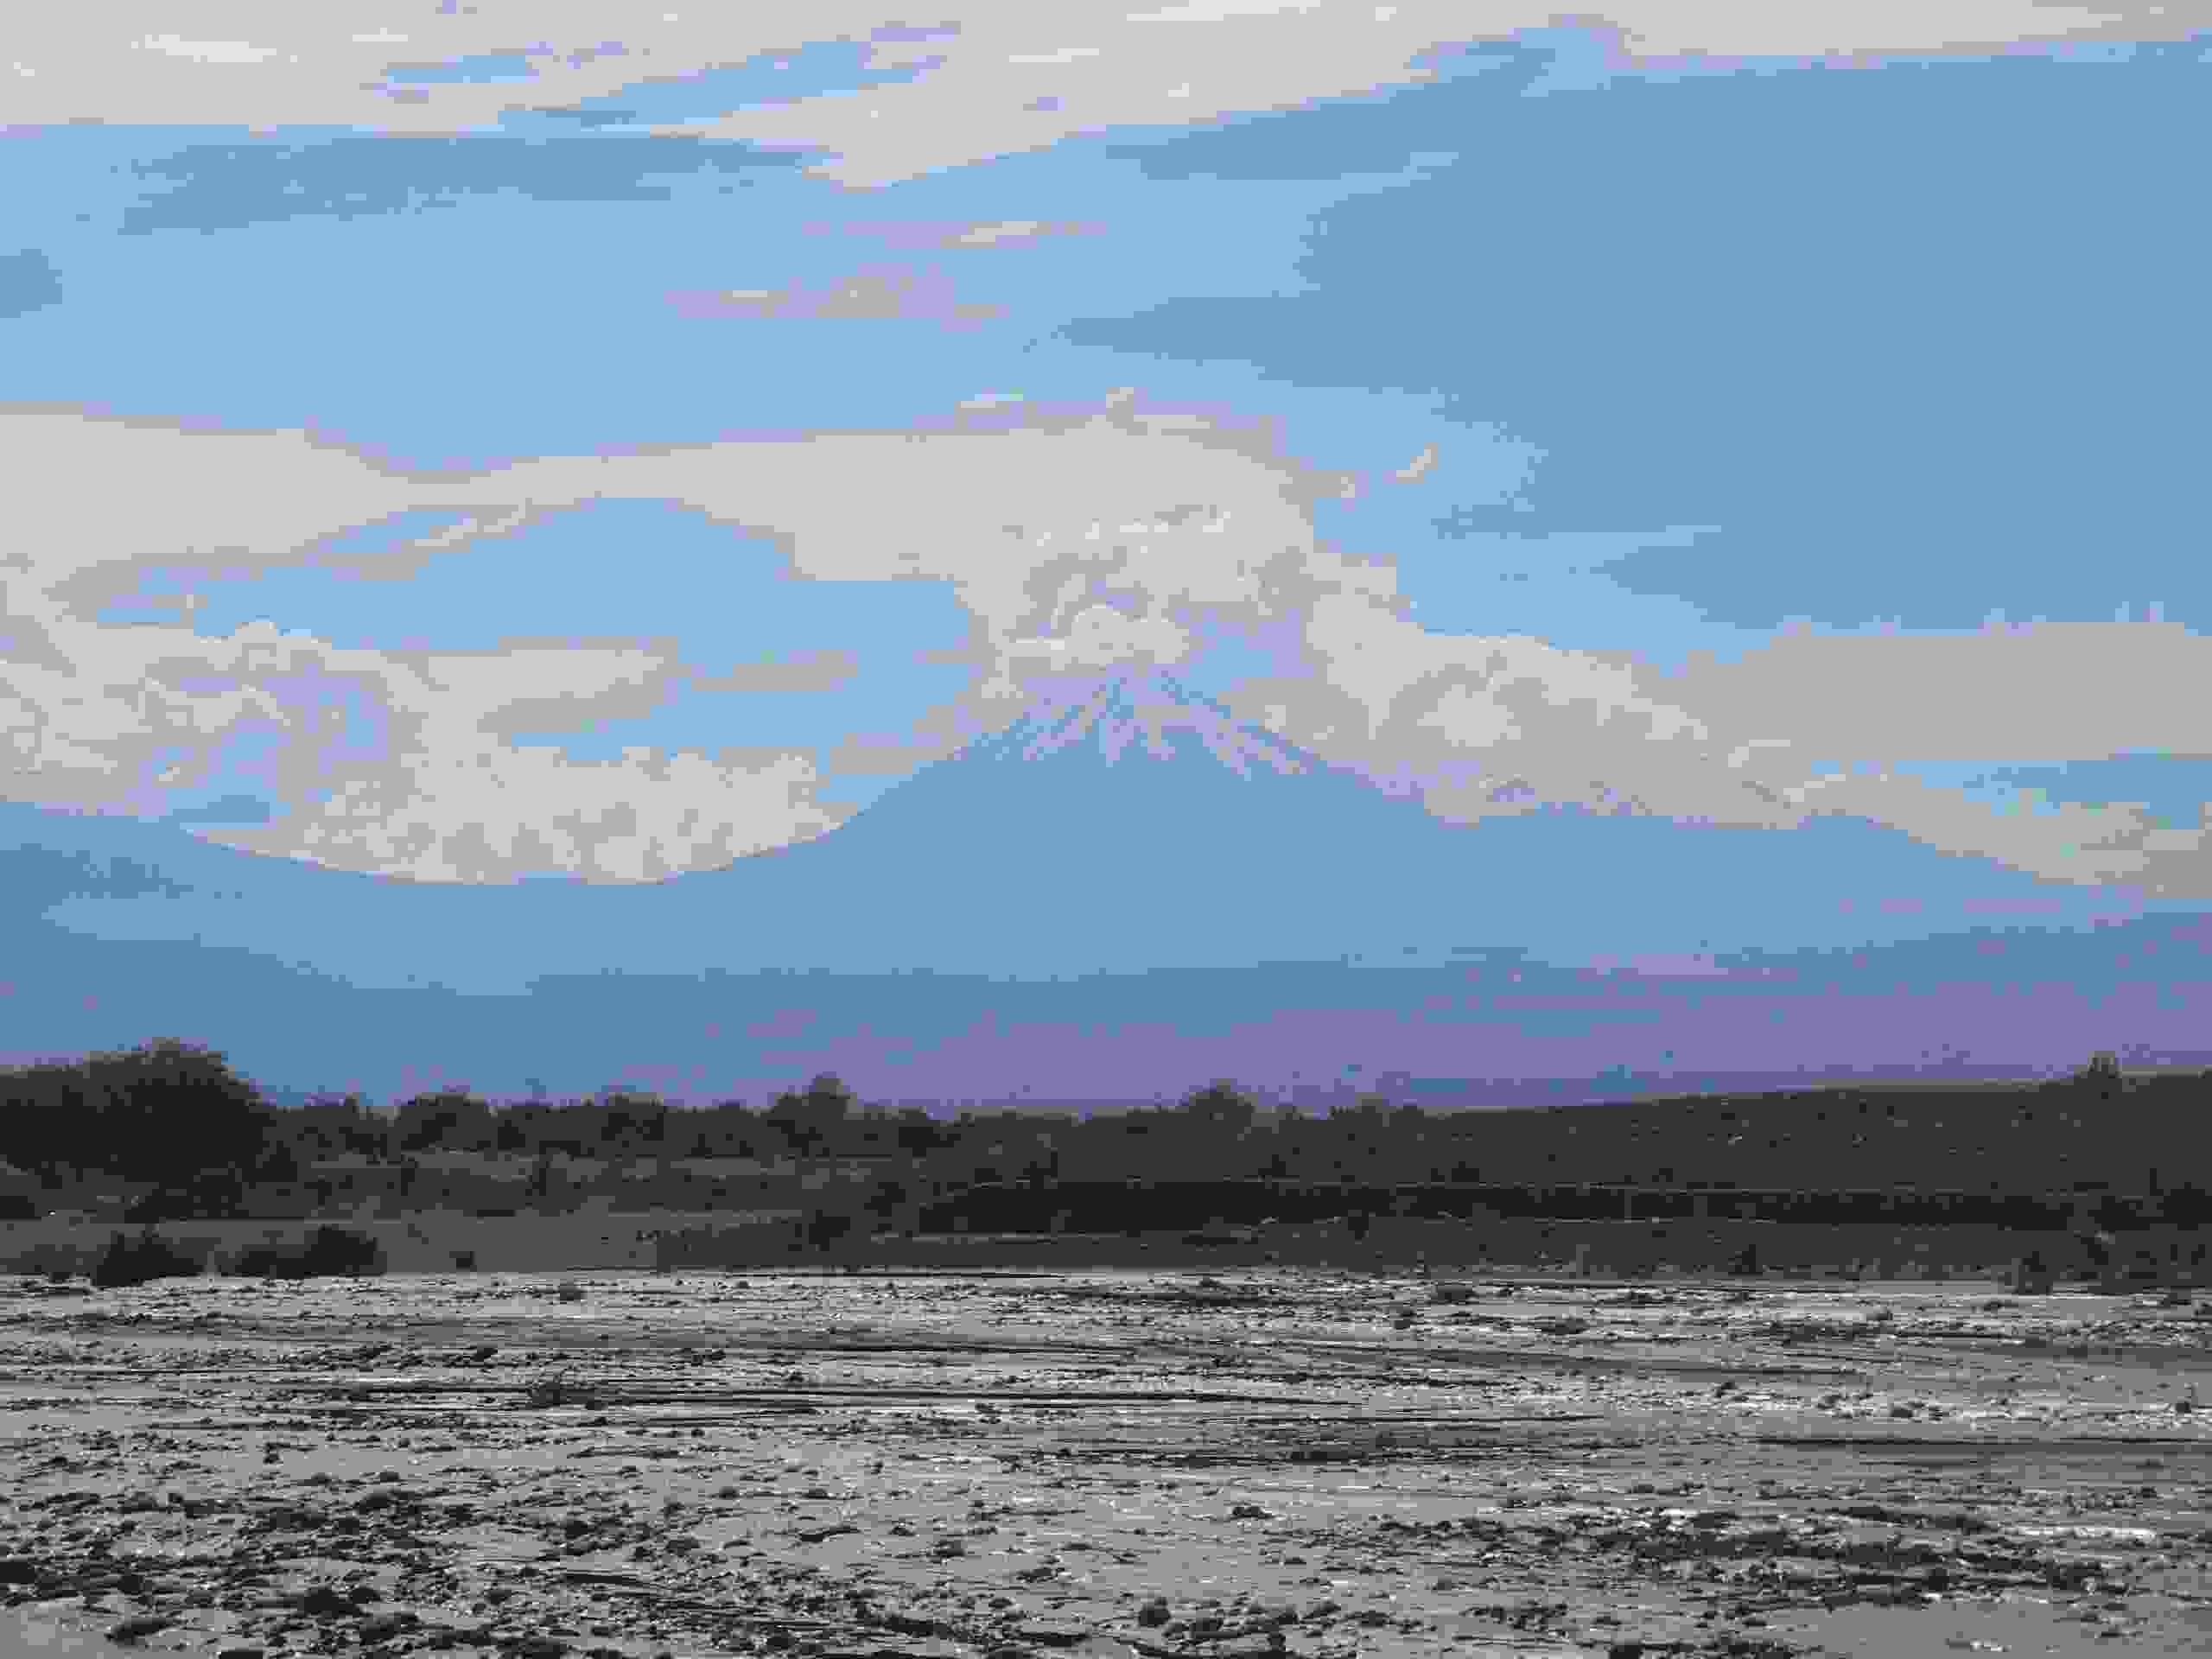
\includegraphics[width=\mywidth]{../wp-content/uploads/2015/04/wpid-wp-1427984374256.jpg} \end{center}

\pagebreak
 Excursion à la vallée de la Lune toute proche.
\begin{center} 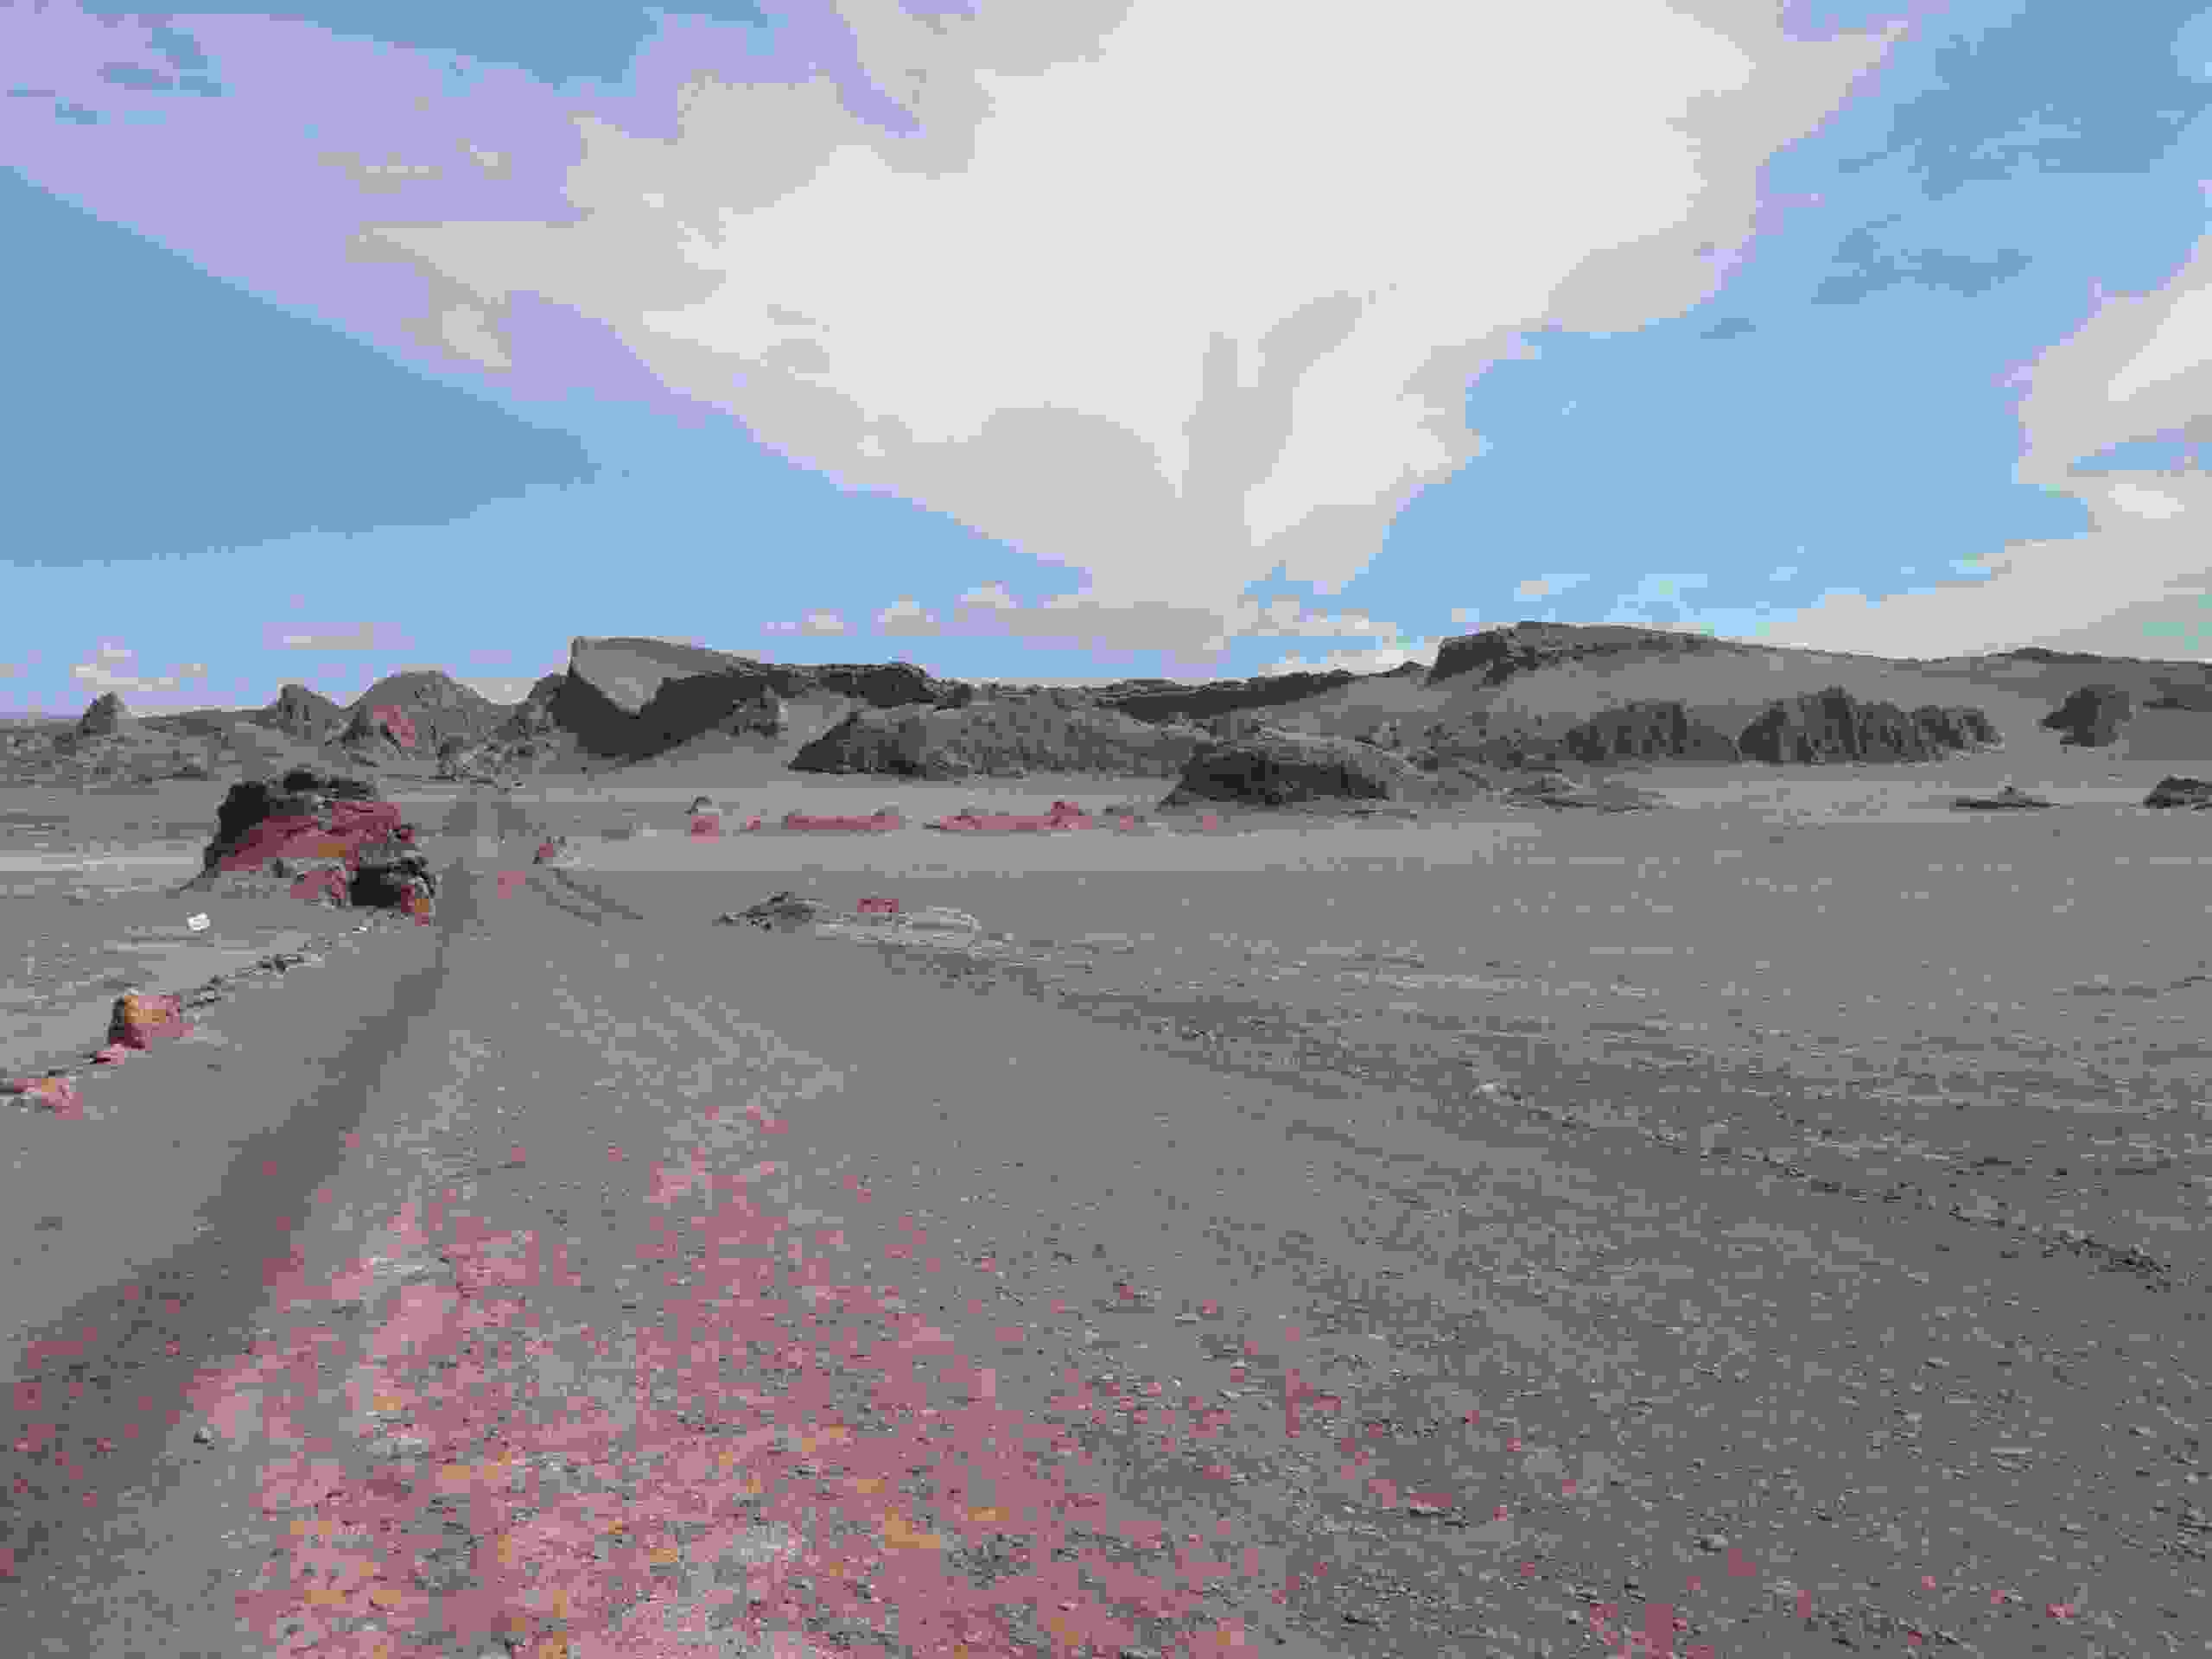
\includegraphics[width=\mywidth]{../wp-content/uploads/2015/04/wpid-wp-1427984406866.jpg} \end{center}
\begin{center} 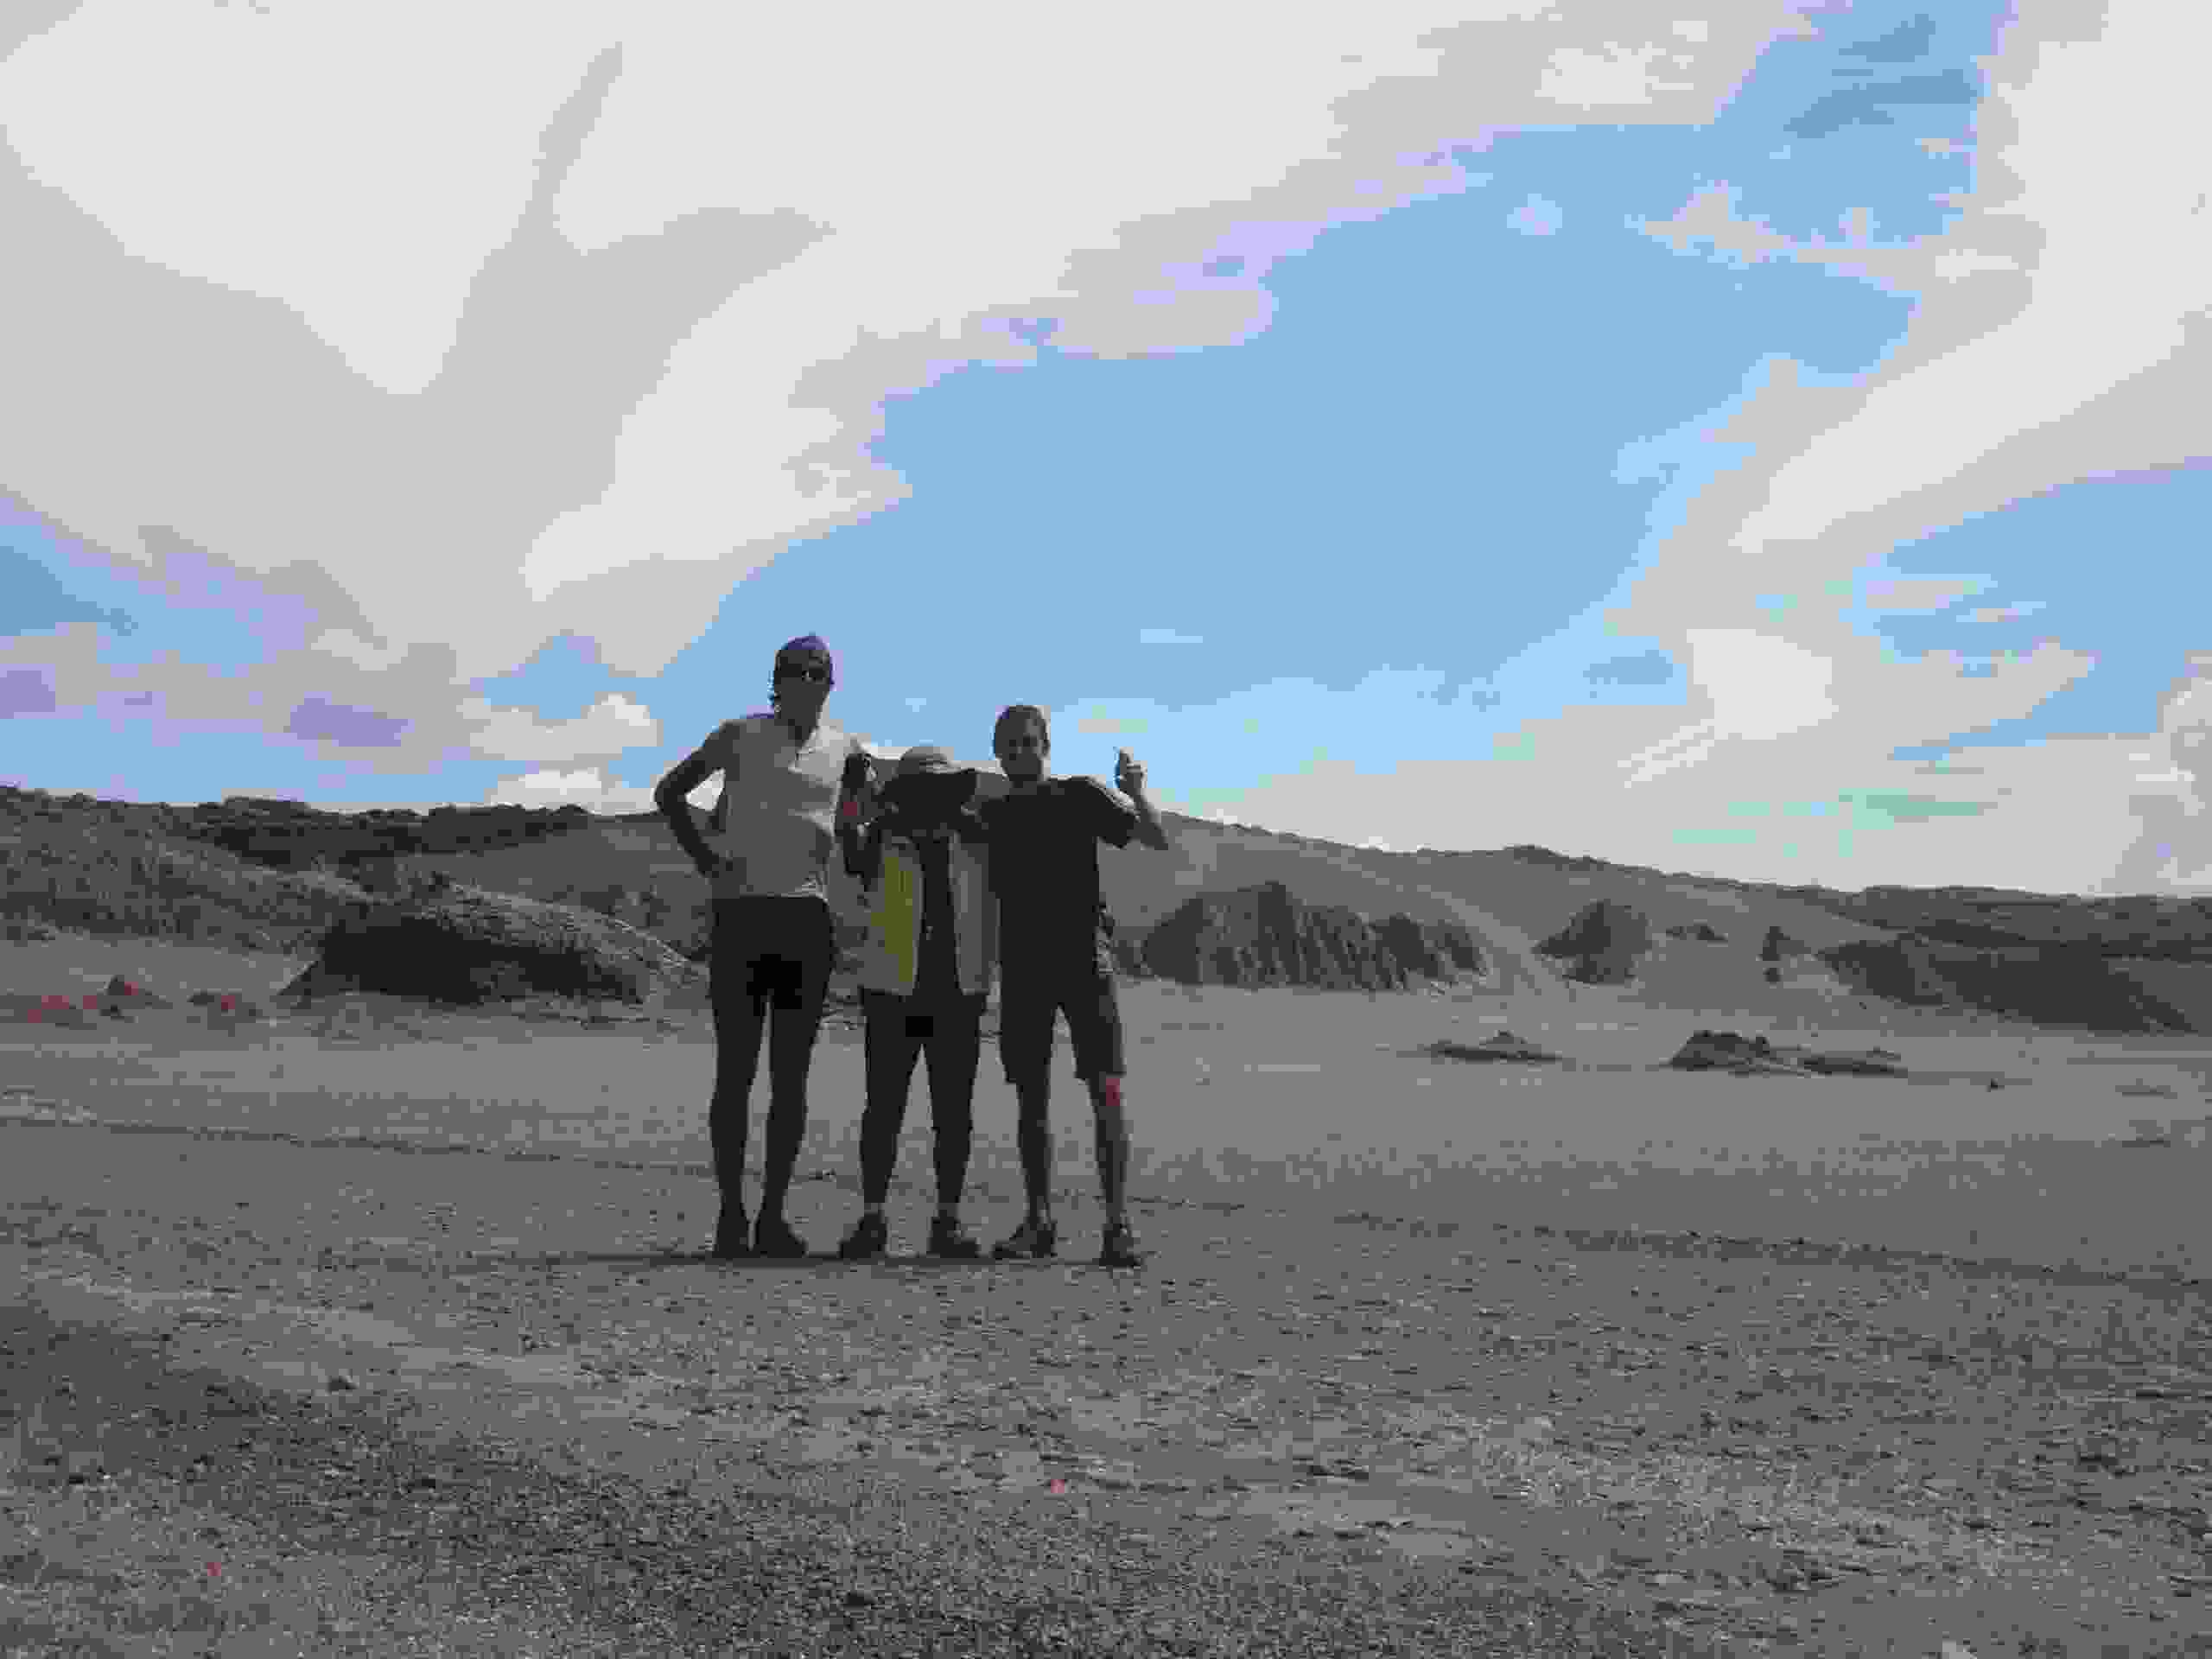
\includegraphics[width=\mywidth]{../wp-content/uploads/2015/04/wpid-wp-1427984342120.jpg} \end{center}

 Puis préparation de la suite : la traversée du Sud Lipez en Bolivie, en compagnie de Lucie et Frédéric qui ont le même itinéraire. 

 D'abord aller chercher des infos sur l'état des pistes et la météo auprès des agences de tour en jeep, puis faire le plein de nourriture pour une dizaine de jours d'autonomie.
\begin{center} 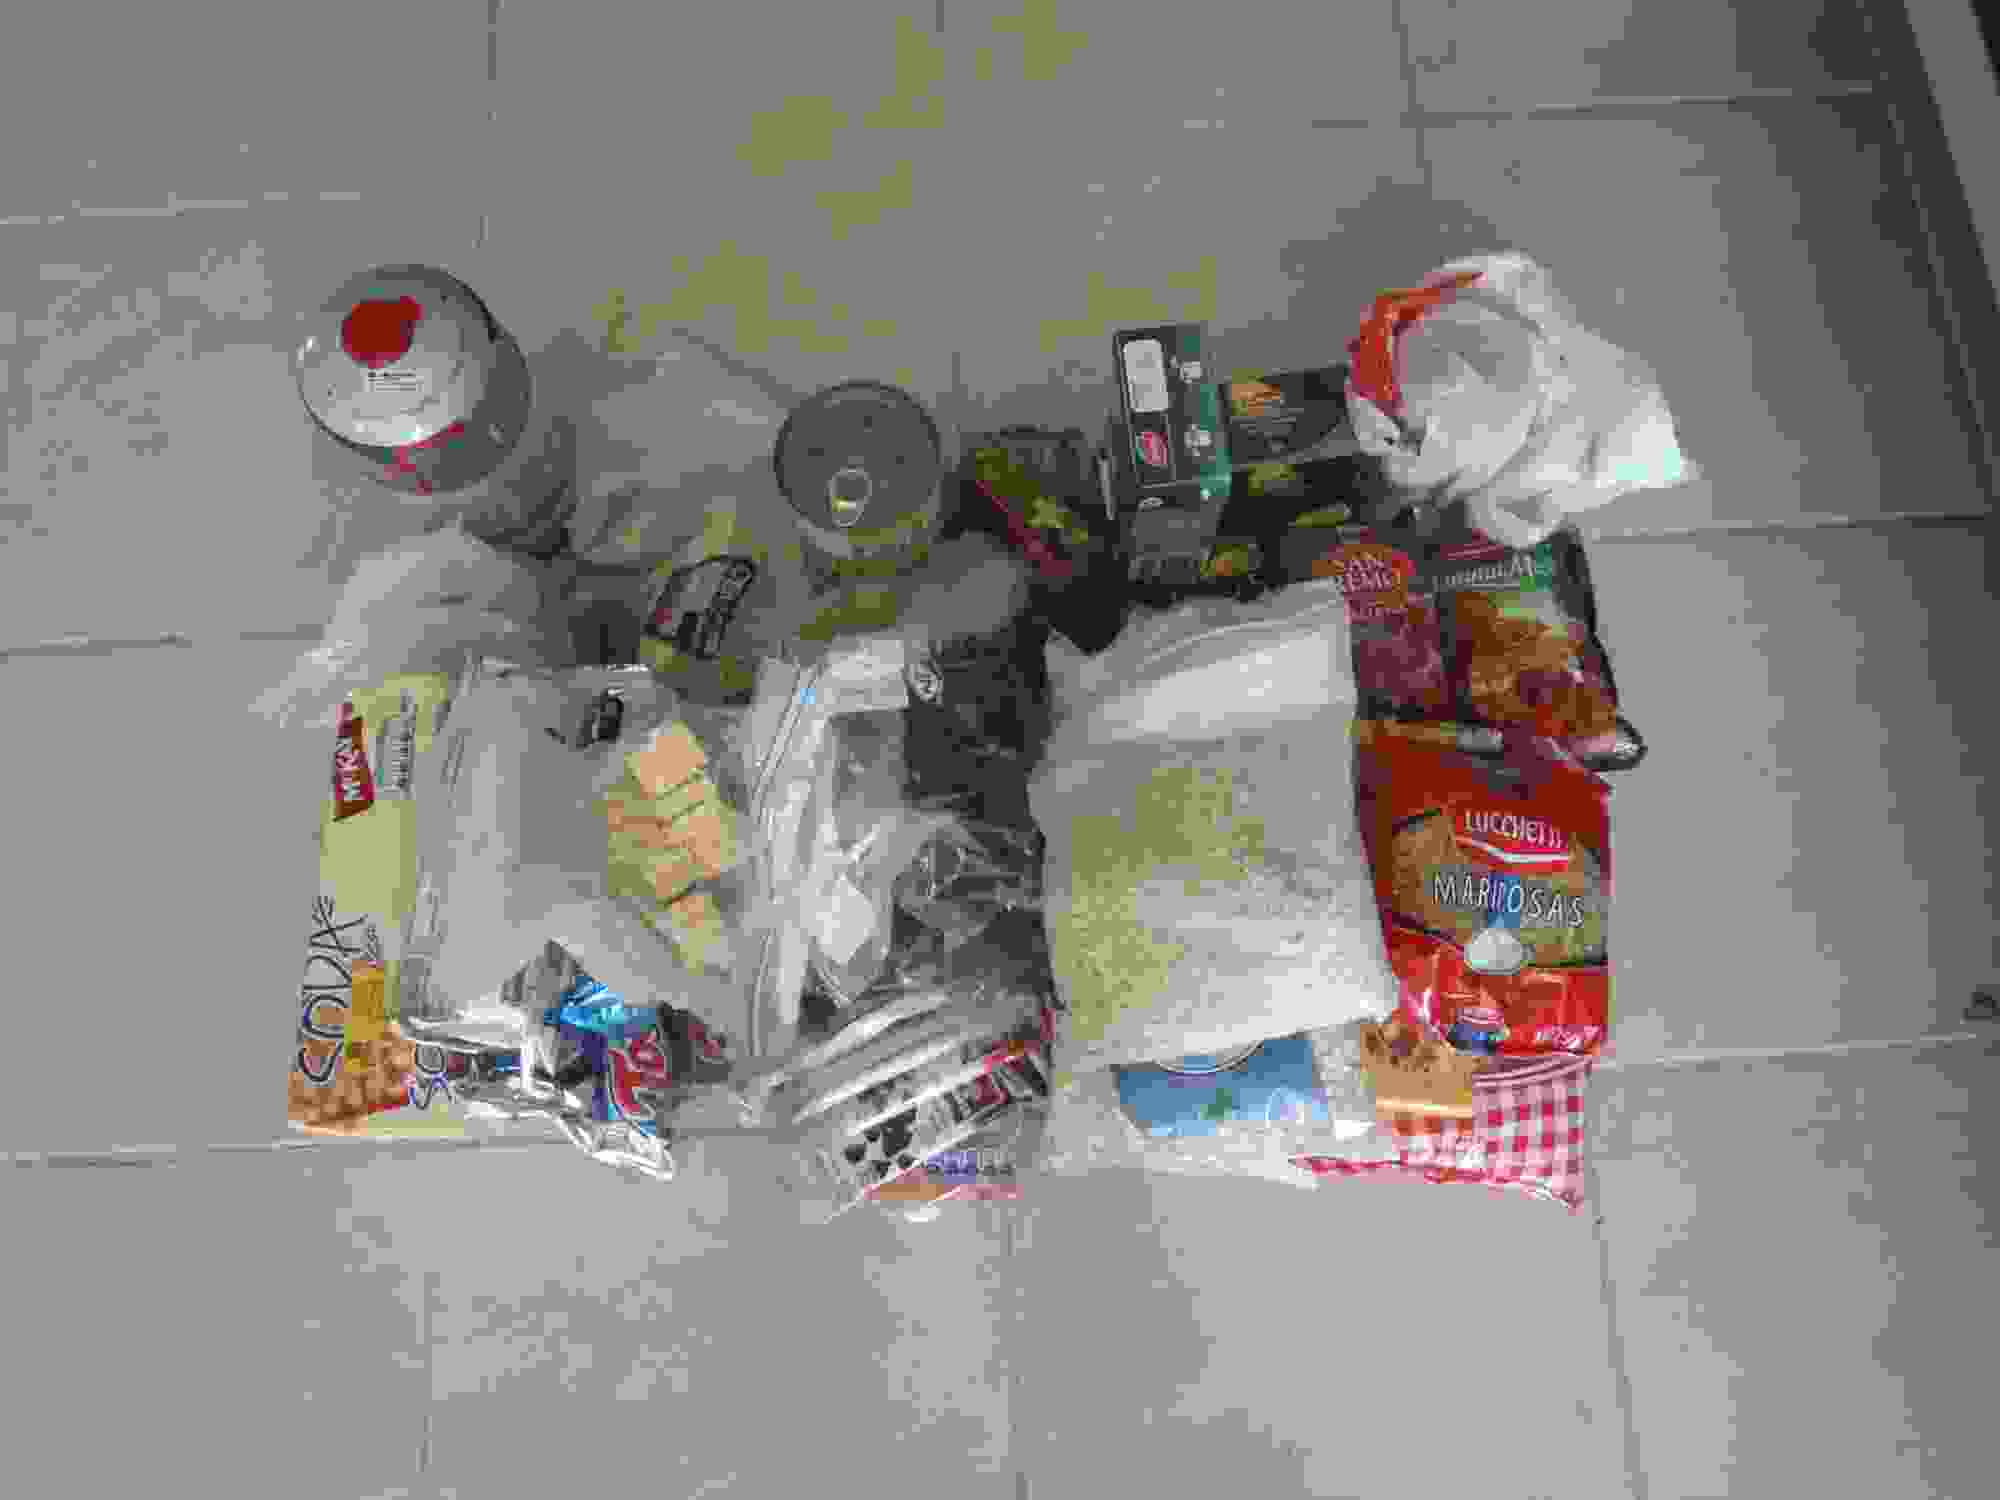
\includegraphics[width=\mywidth]{../wp-content/uploads/2015/04/wpid-wp-1427986446964.jpg} \end{center}

\subsection*{1\ier\ jour} 
 Passage à la douane chilienne et montée à 4600m à la frontière bolivienne à l'entrée du Sud Lipez : en stop dans un camping-car de touristes américains, pas besoin de s'épuiser d'entrée la suite sera assez difficile.
\begin{center} 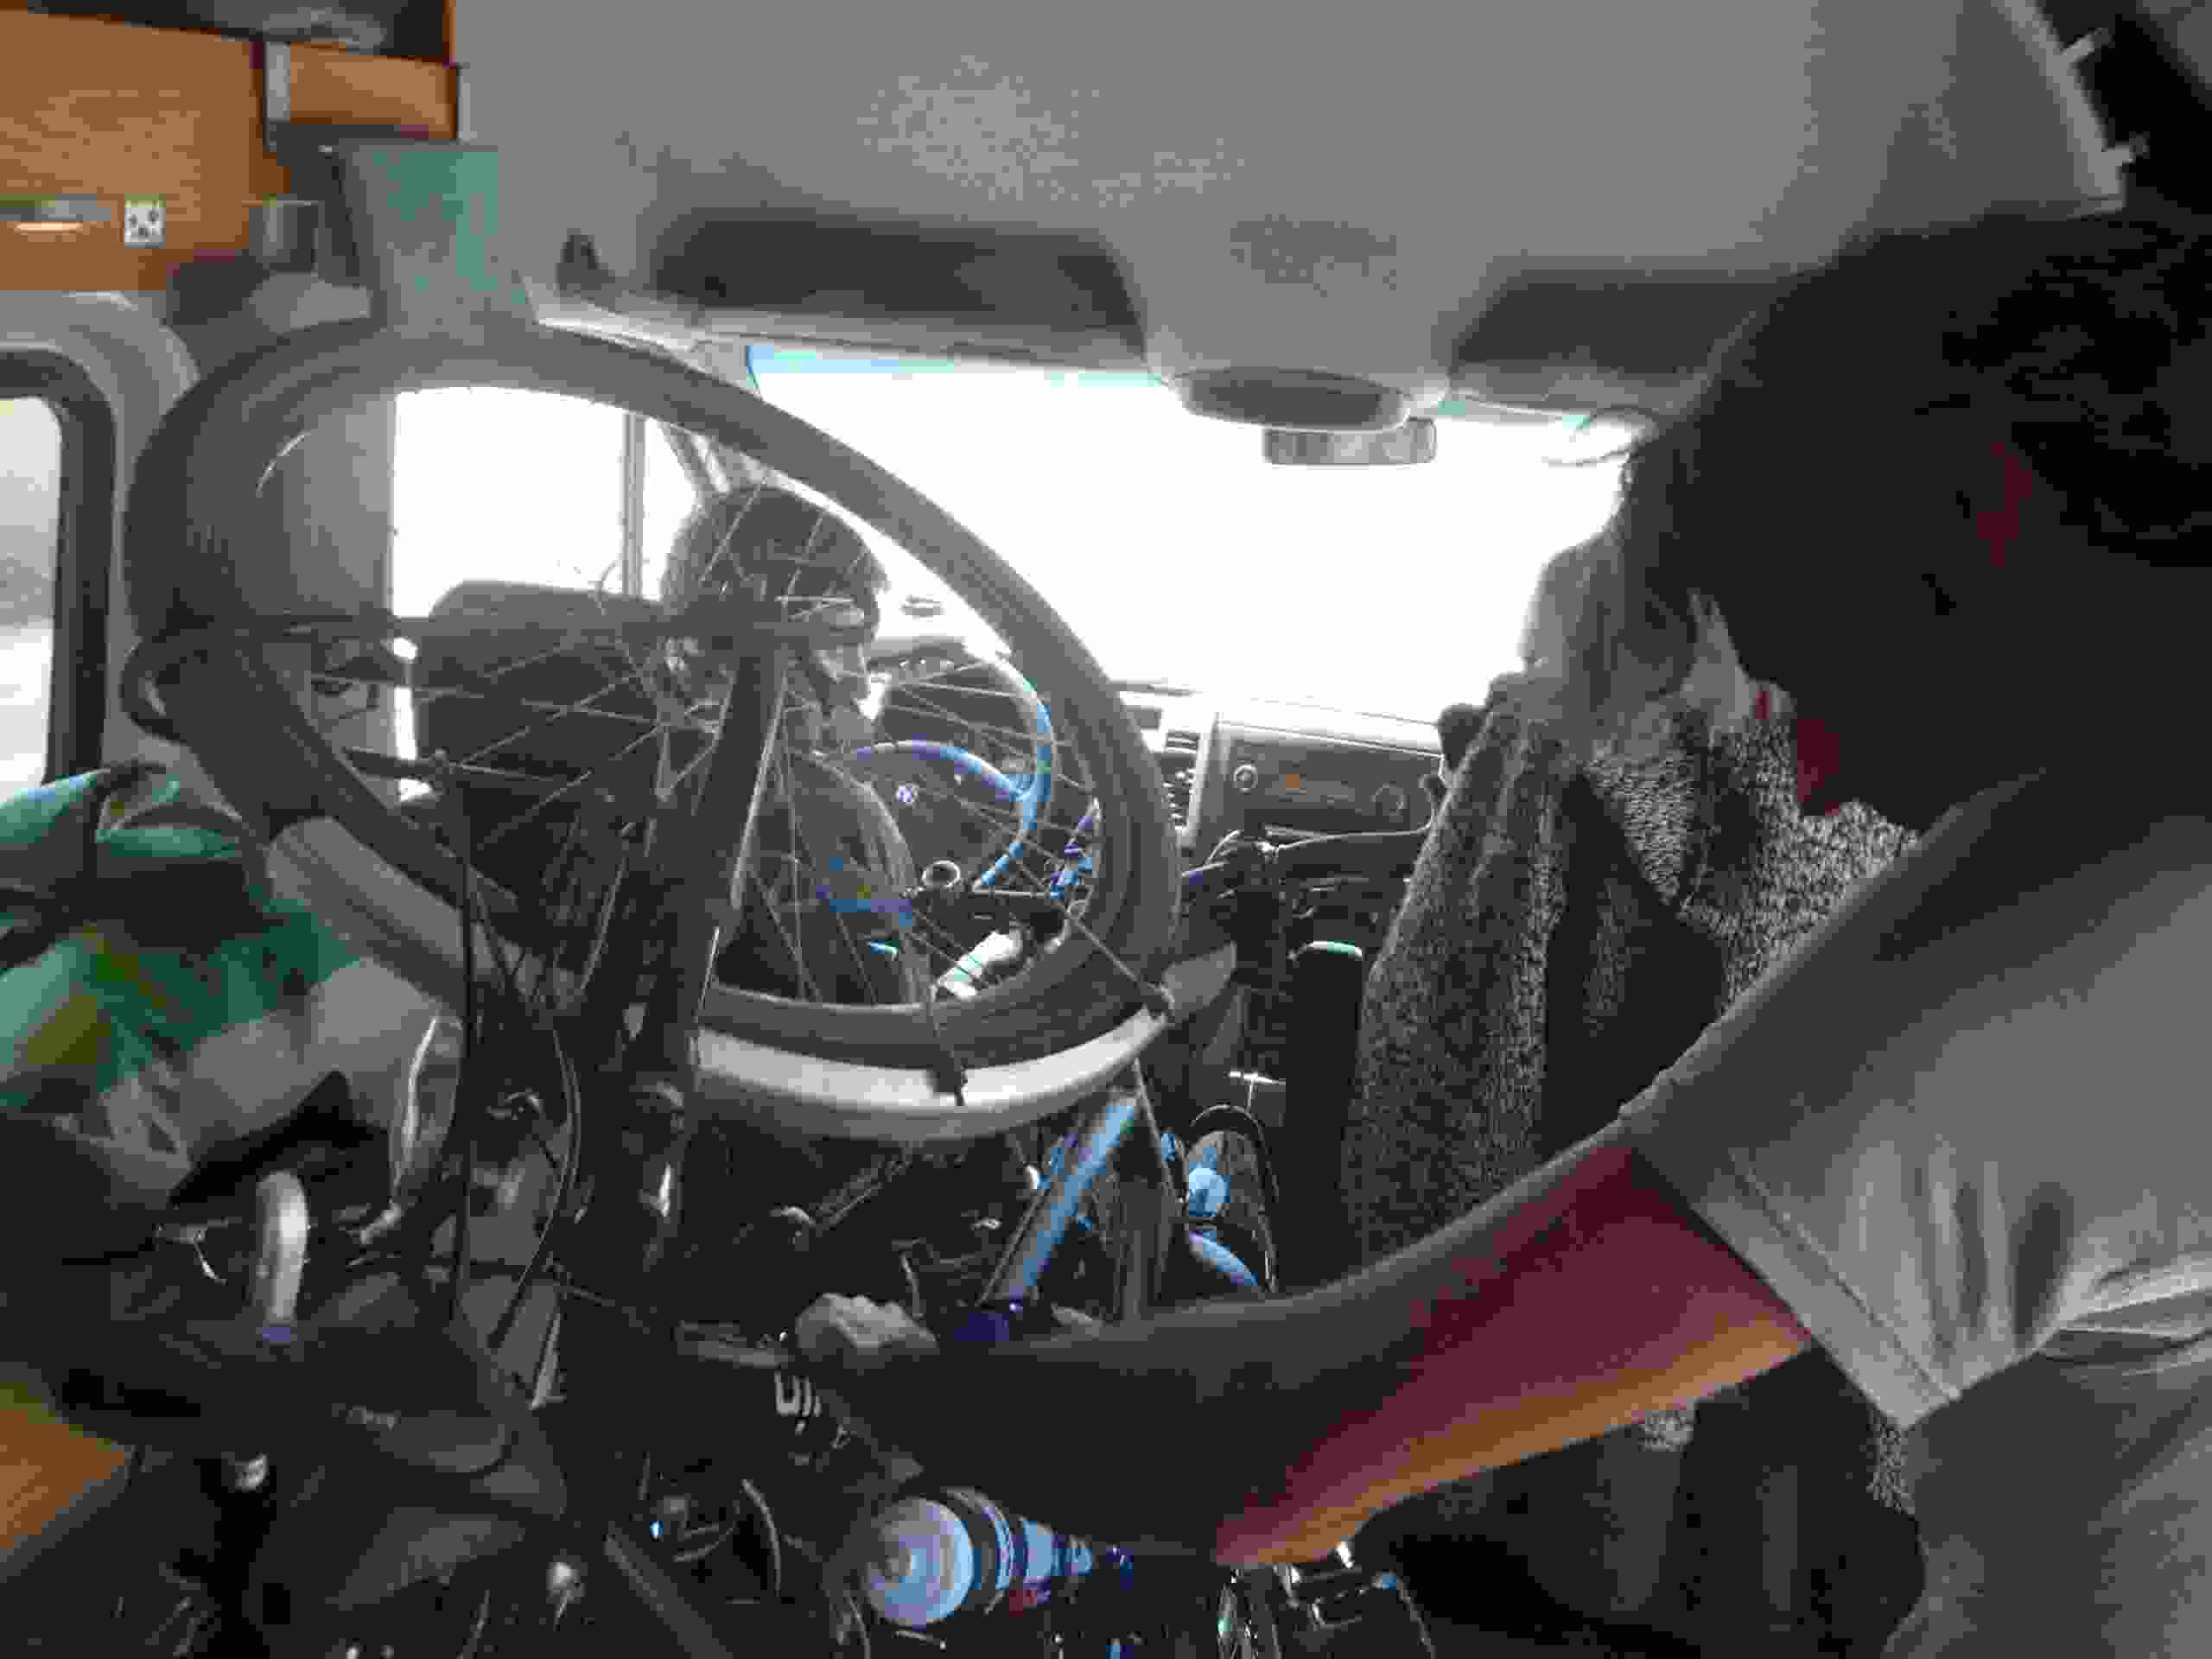
\includegraphics[width=\mywidth]{../wp-content/uploads/2015/04/wpid-wp-1427943860712.jpg} \end{center}
\begin{center} 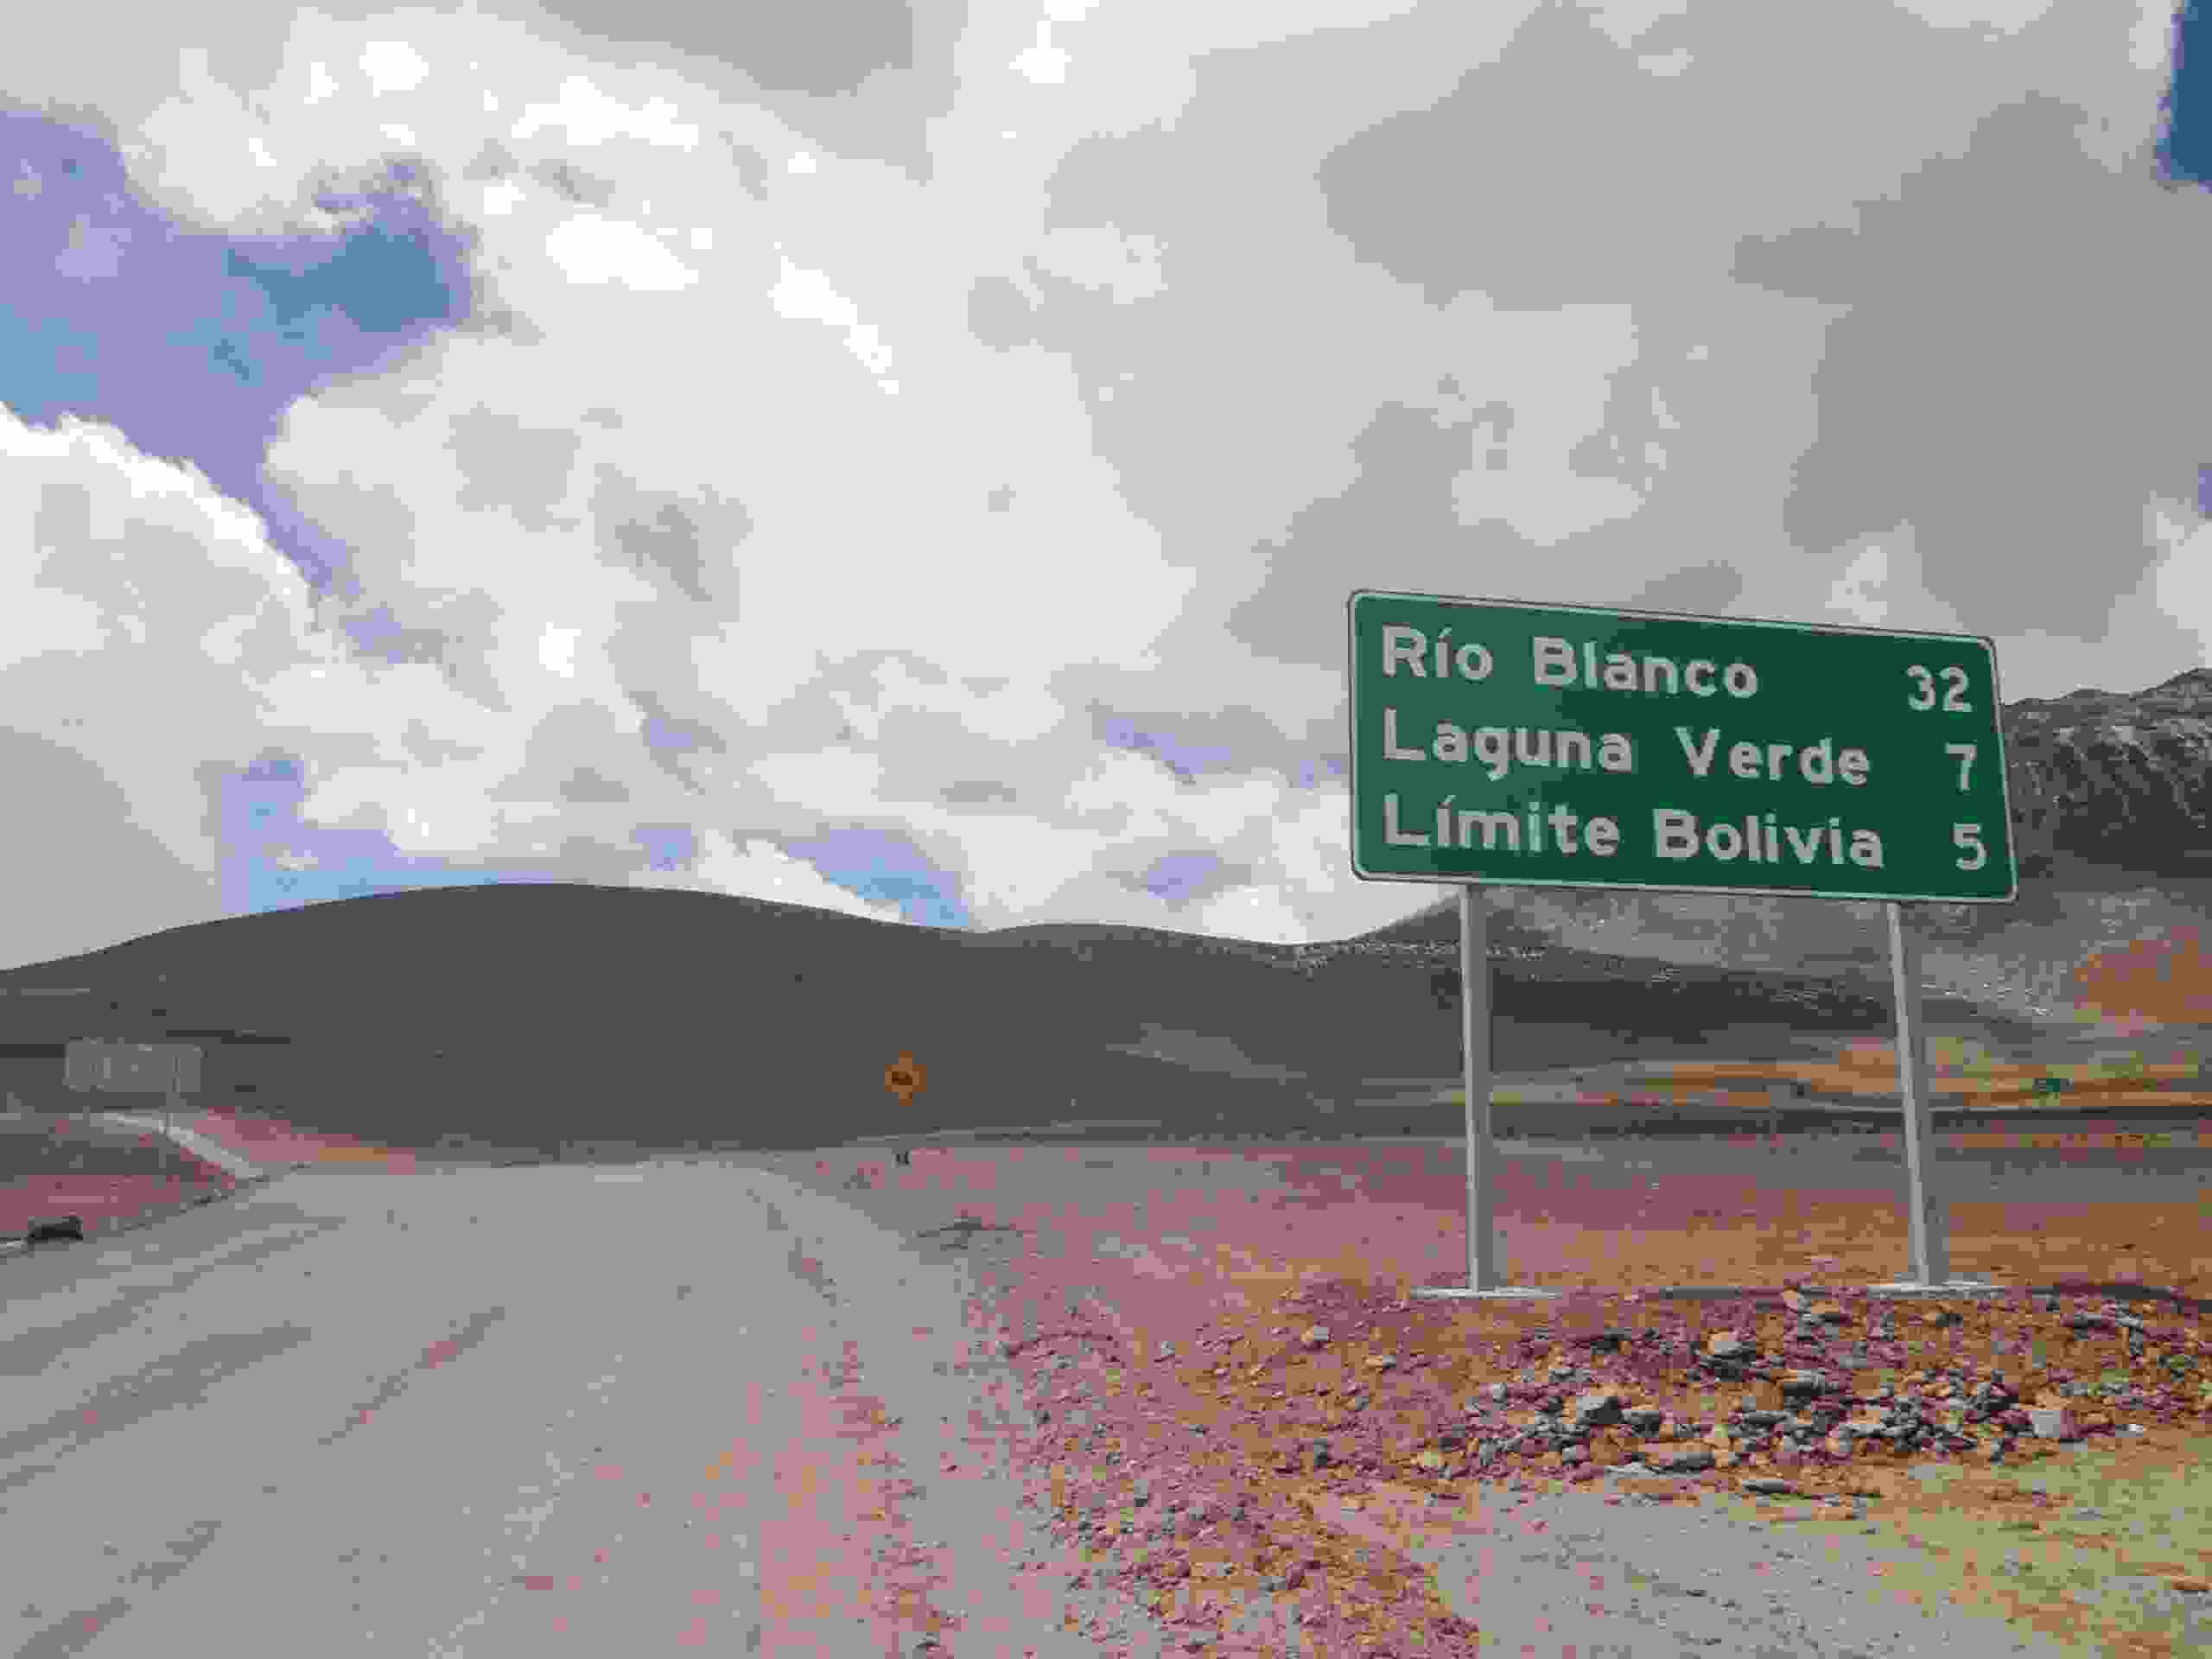
\includegraphics[width=\mywidth]{../wp-content/uploads/2015/04/wpid-wp-1427943860696.jpg} \end{center}

 On arrive assez rapidement à la Laguna Blanca puis à la Laguna Verde.
\begin{center} 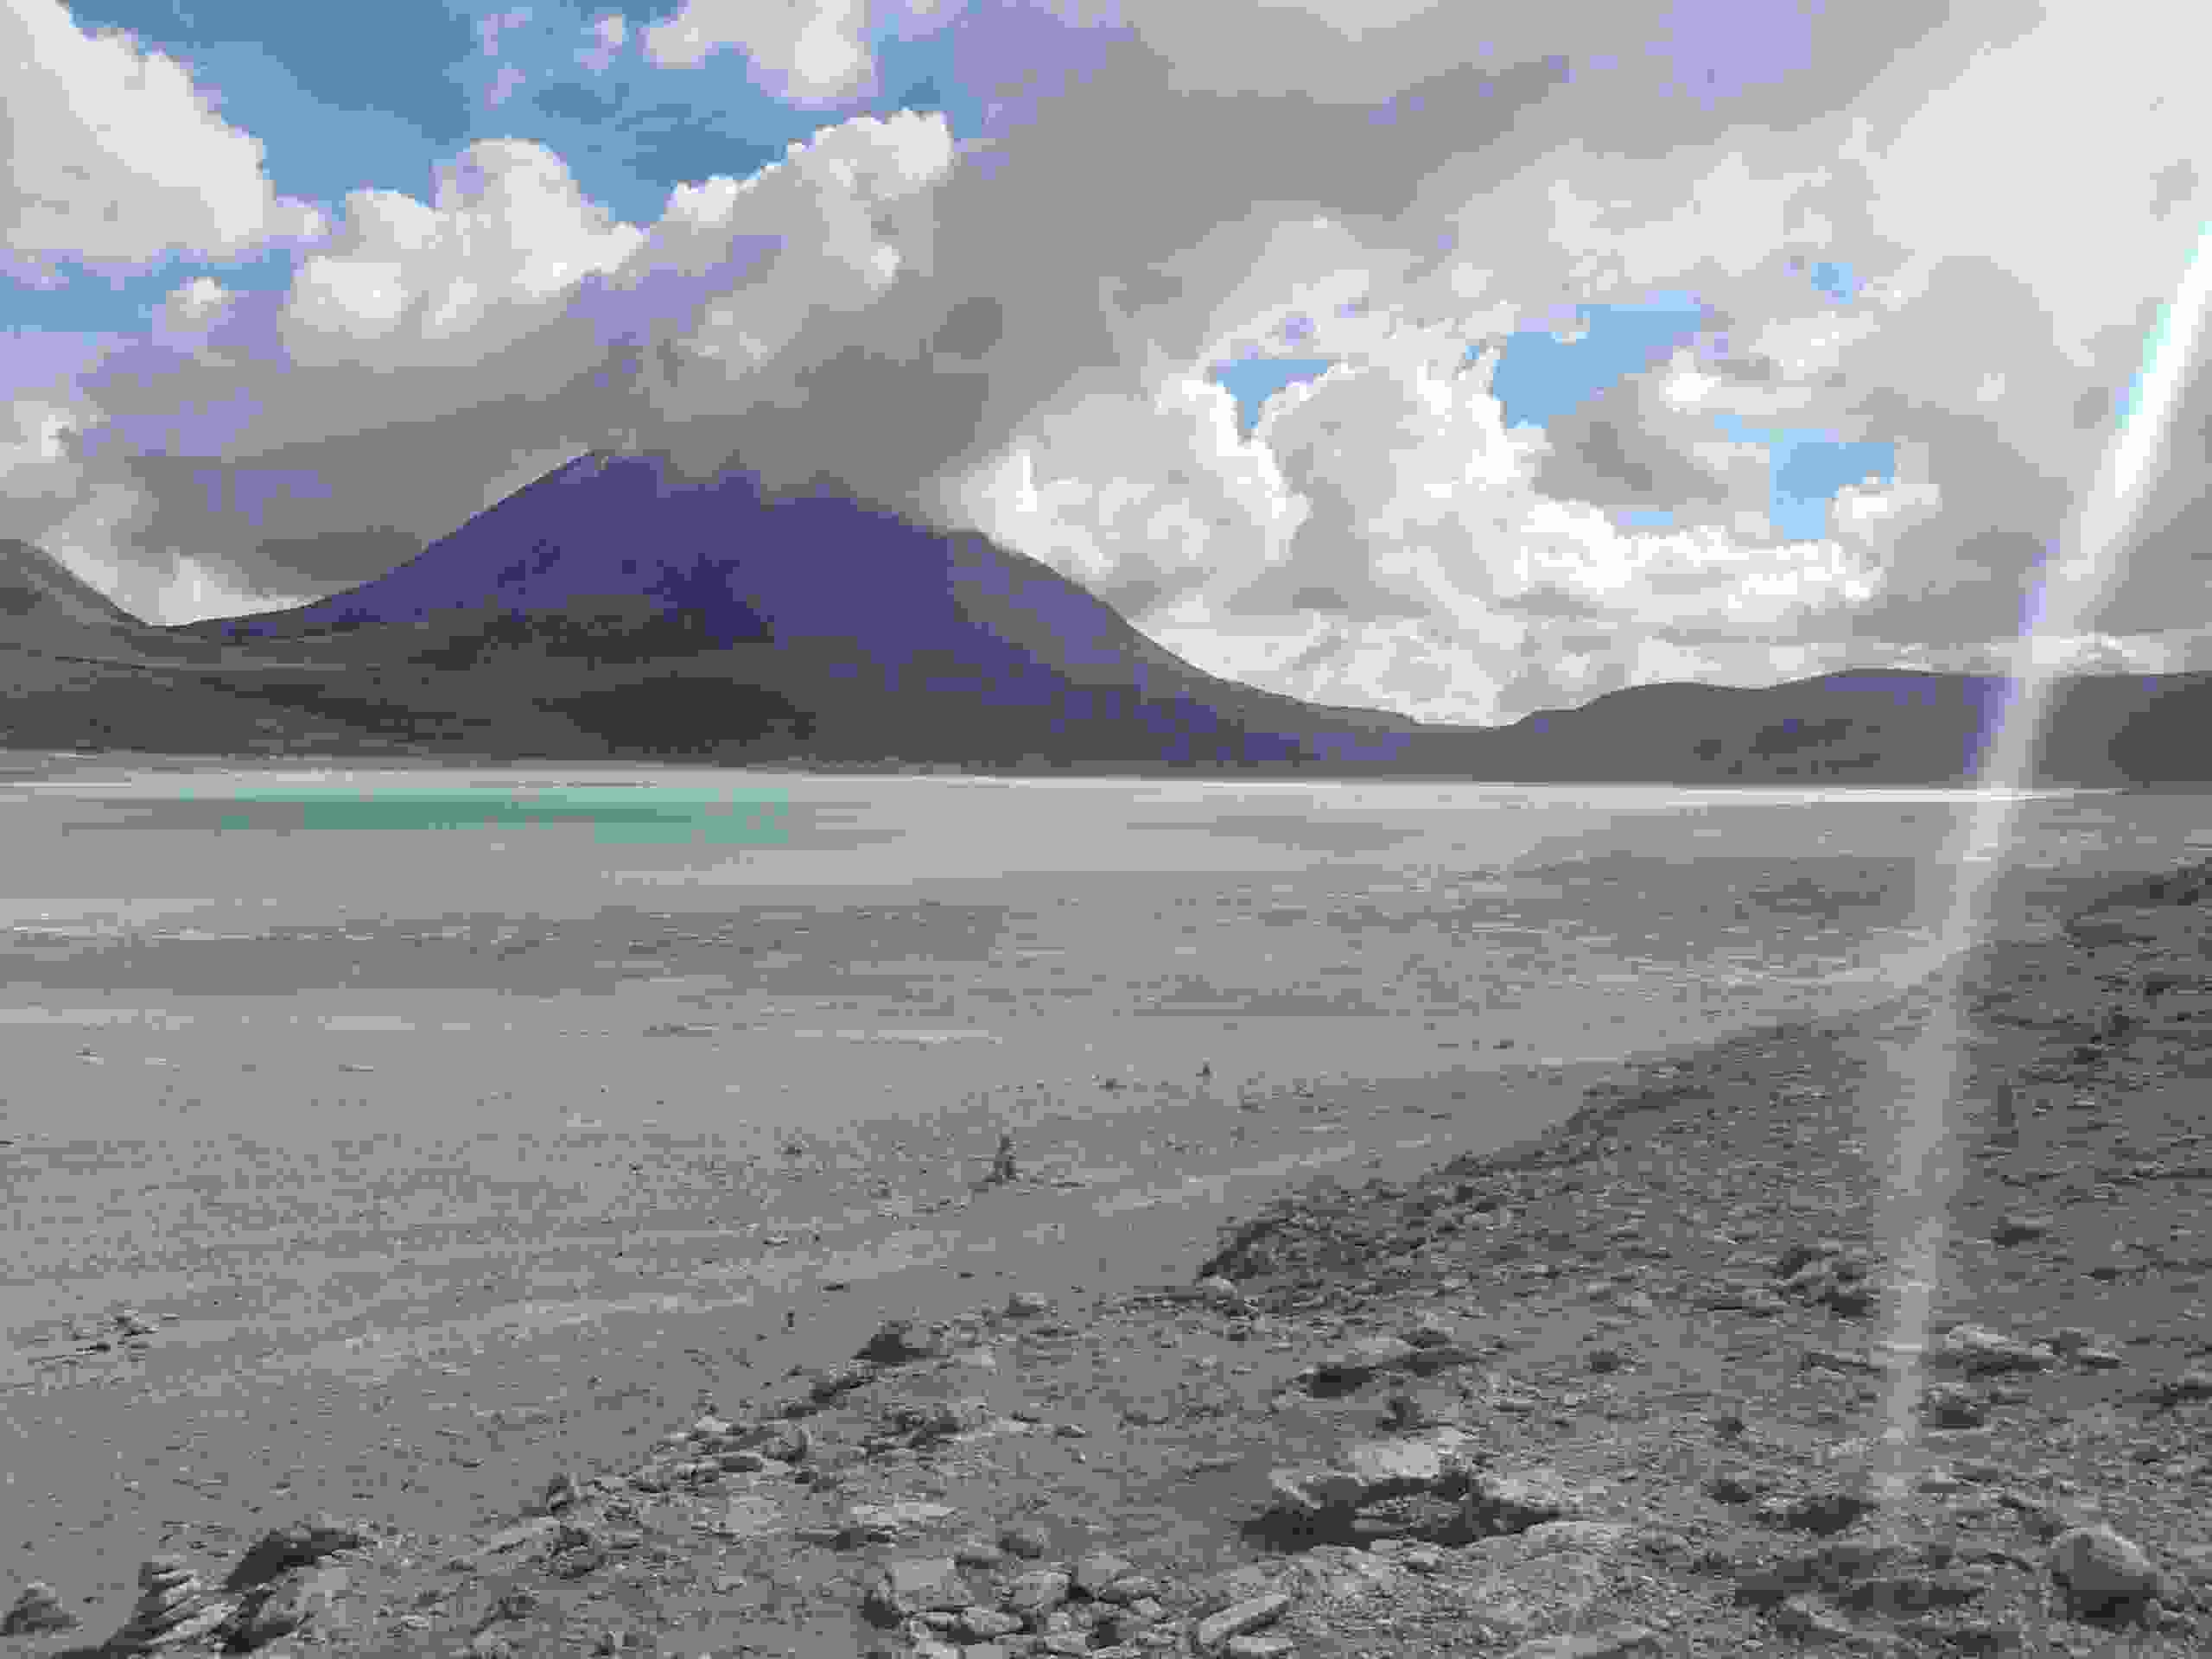
\includegraphics[width=\mywidth]{../wp-content/uploads/2015/04/wpid-wp-1427943860676.jpg} \end{center}
% image en double...
%\begin{center} 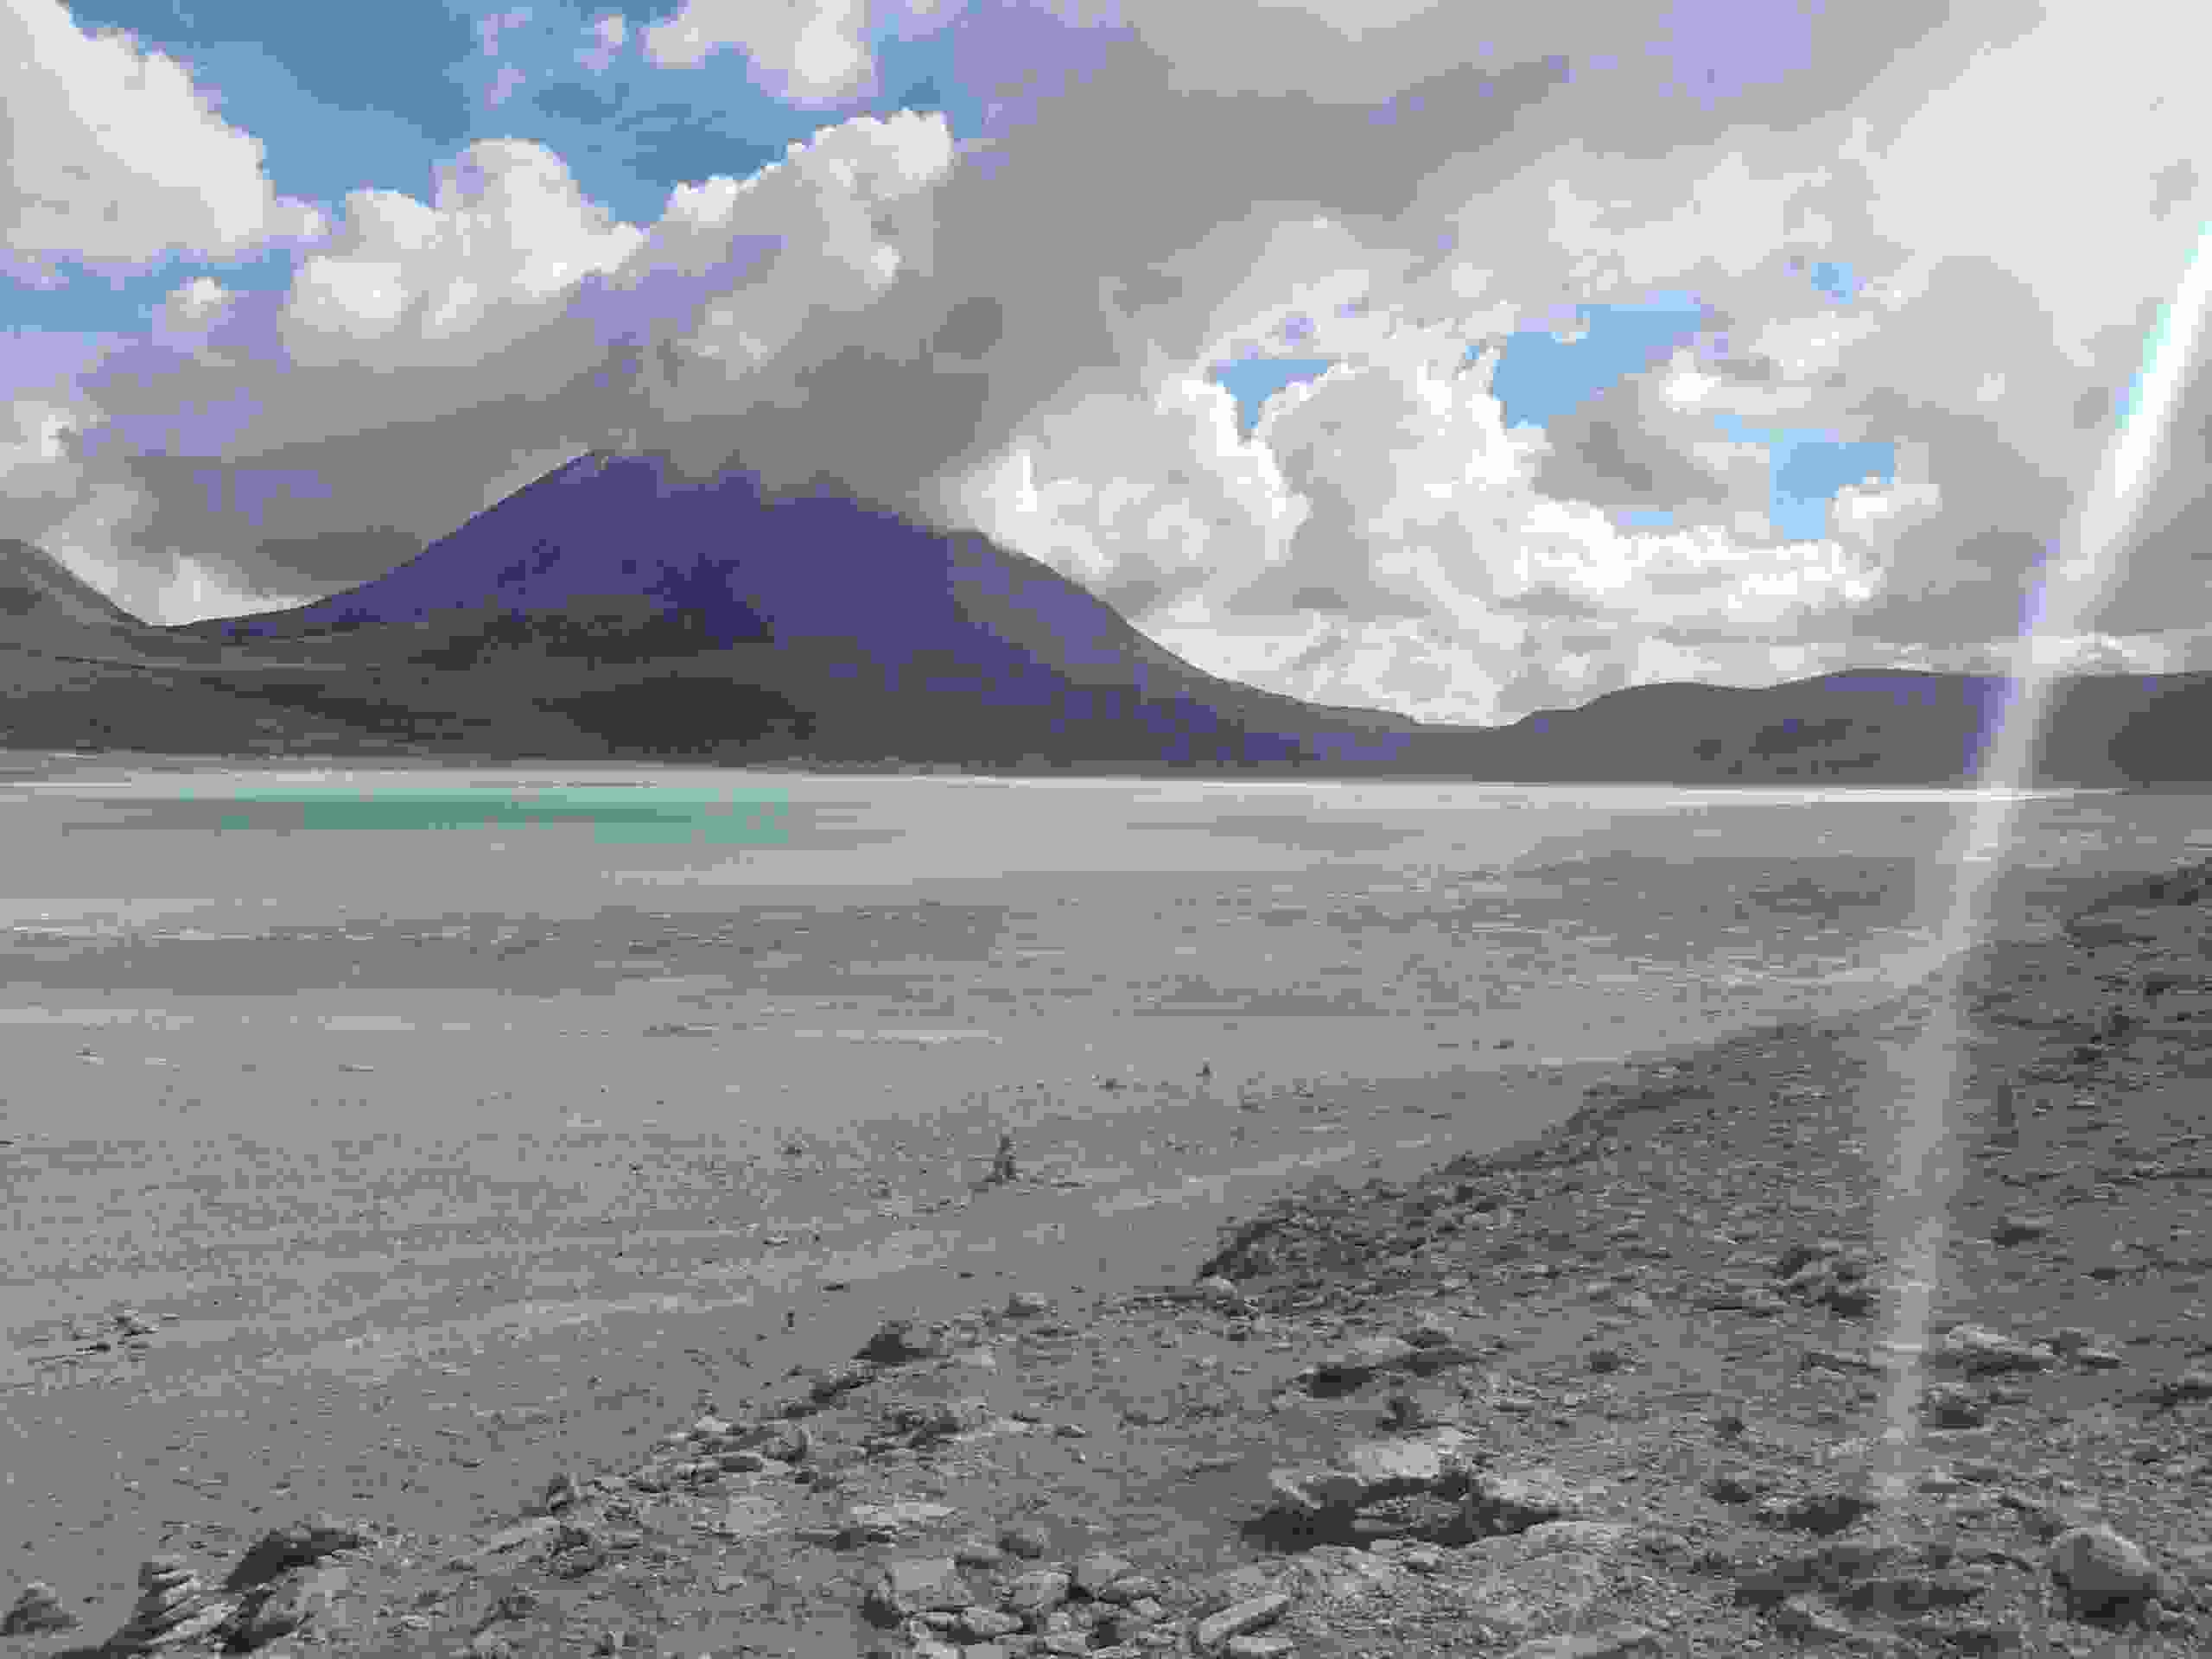
\includegraphics[width=\mywidth]{../wp-content/uploads/2015/04/wpid-wp-1427983994198.jpg} \end{center}

\pagebreak
 Bivouac dans une maison en ruine :
\begin{center} 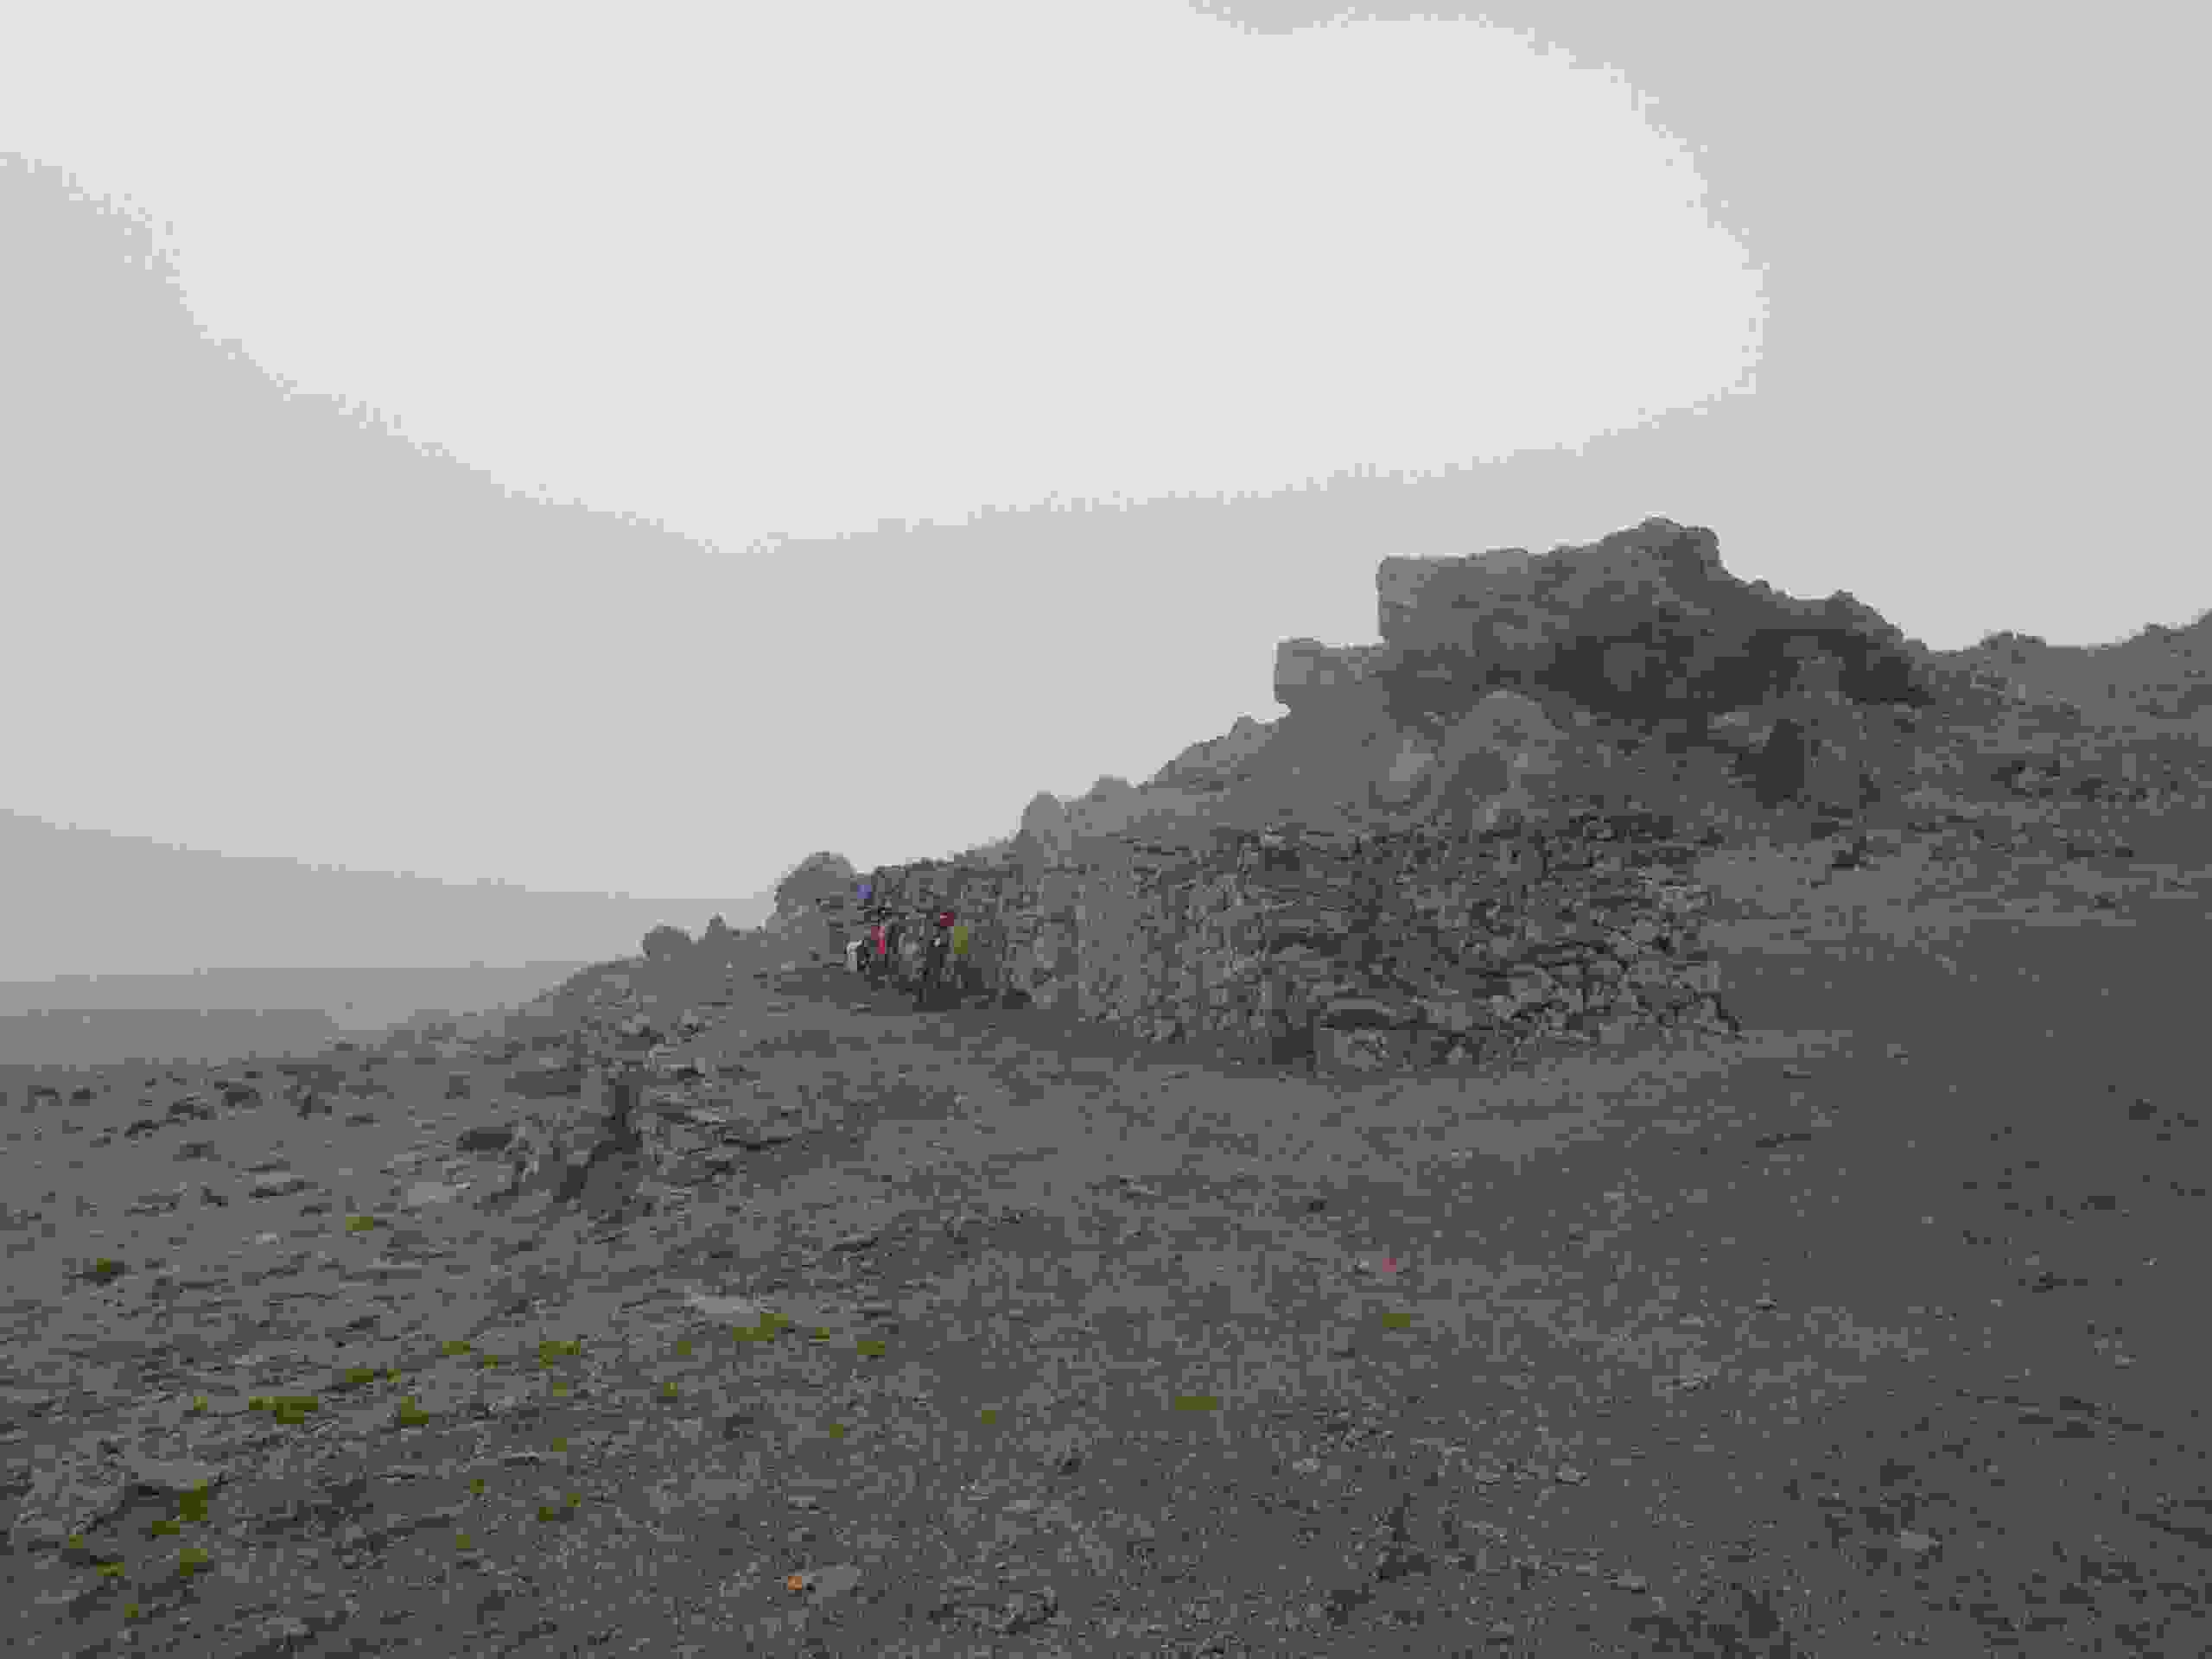
\includegraphics[width=\mywidth]{../wp-content/uploads/2015/04/wpid-wp-1427984018829.jpg} \end{center}

\subsection*{2\ieme\ jour} 
 Lever dans la brume, les jeeps de touristes passent devant nous.
\begin{center} 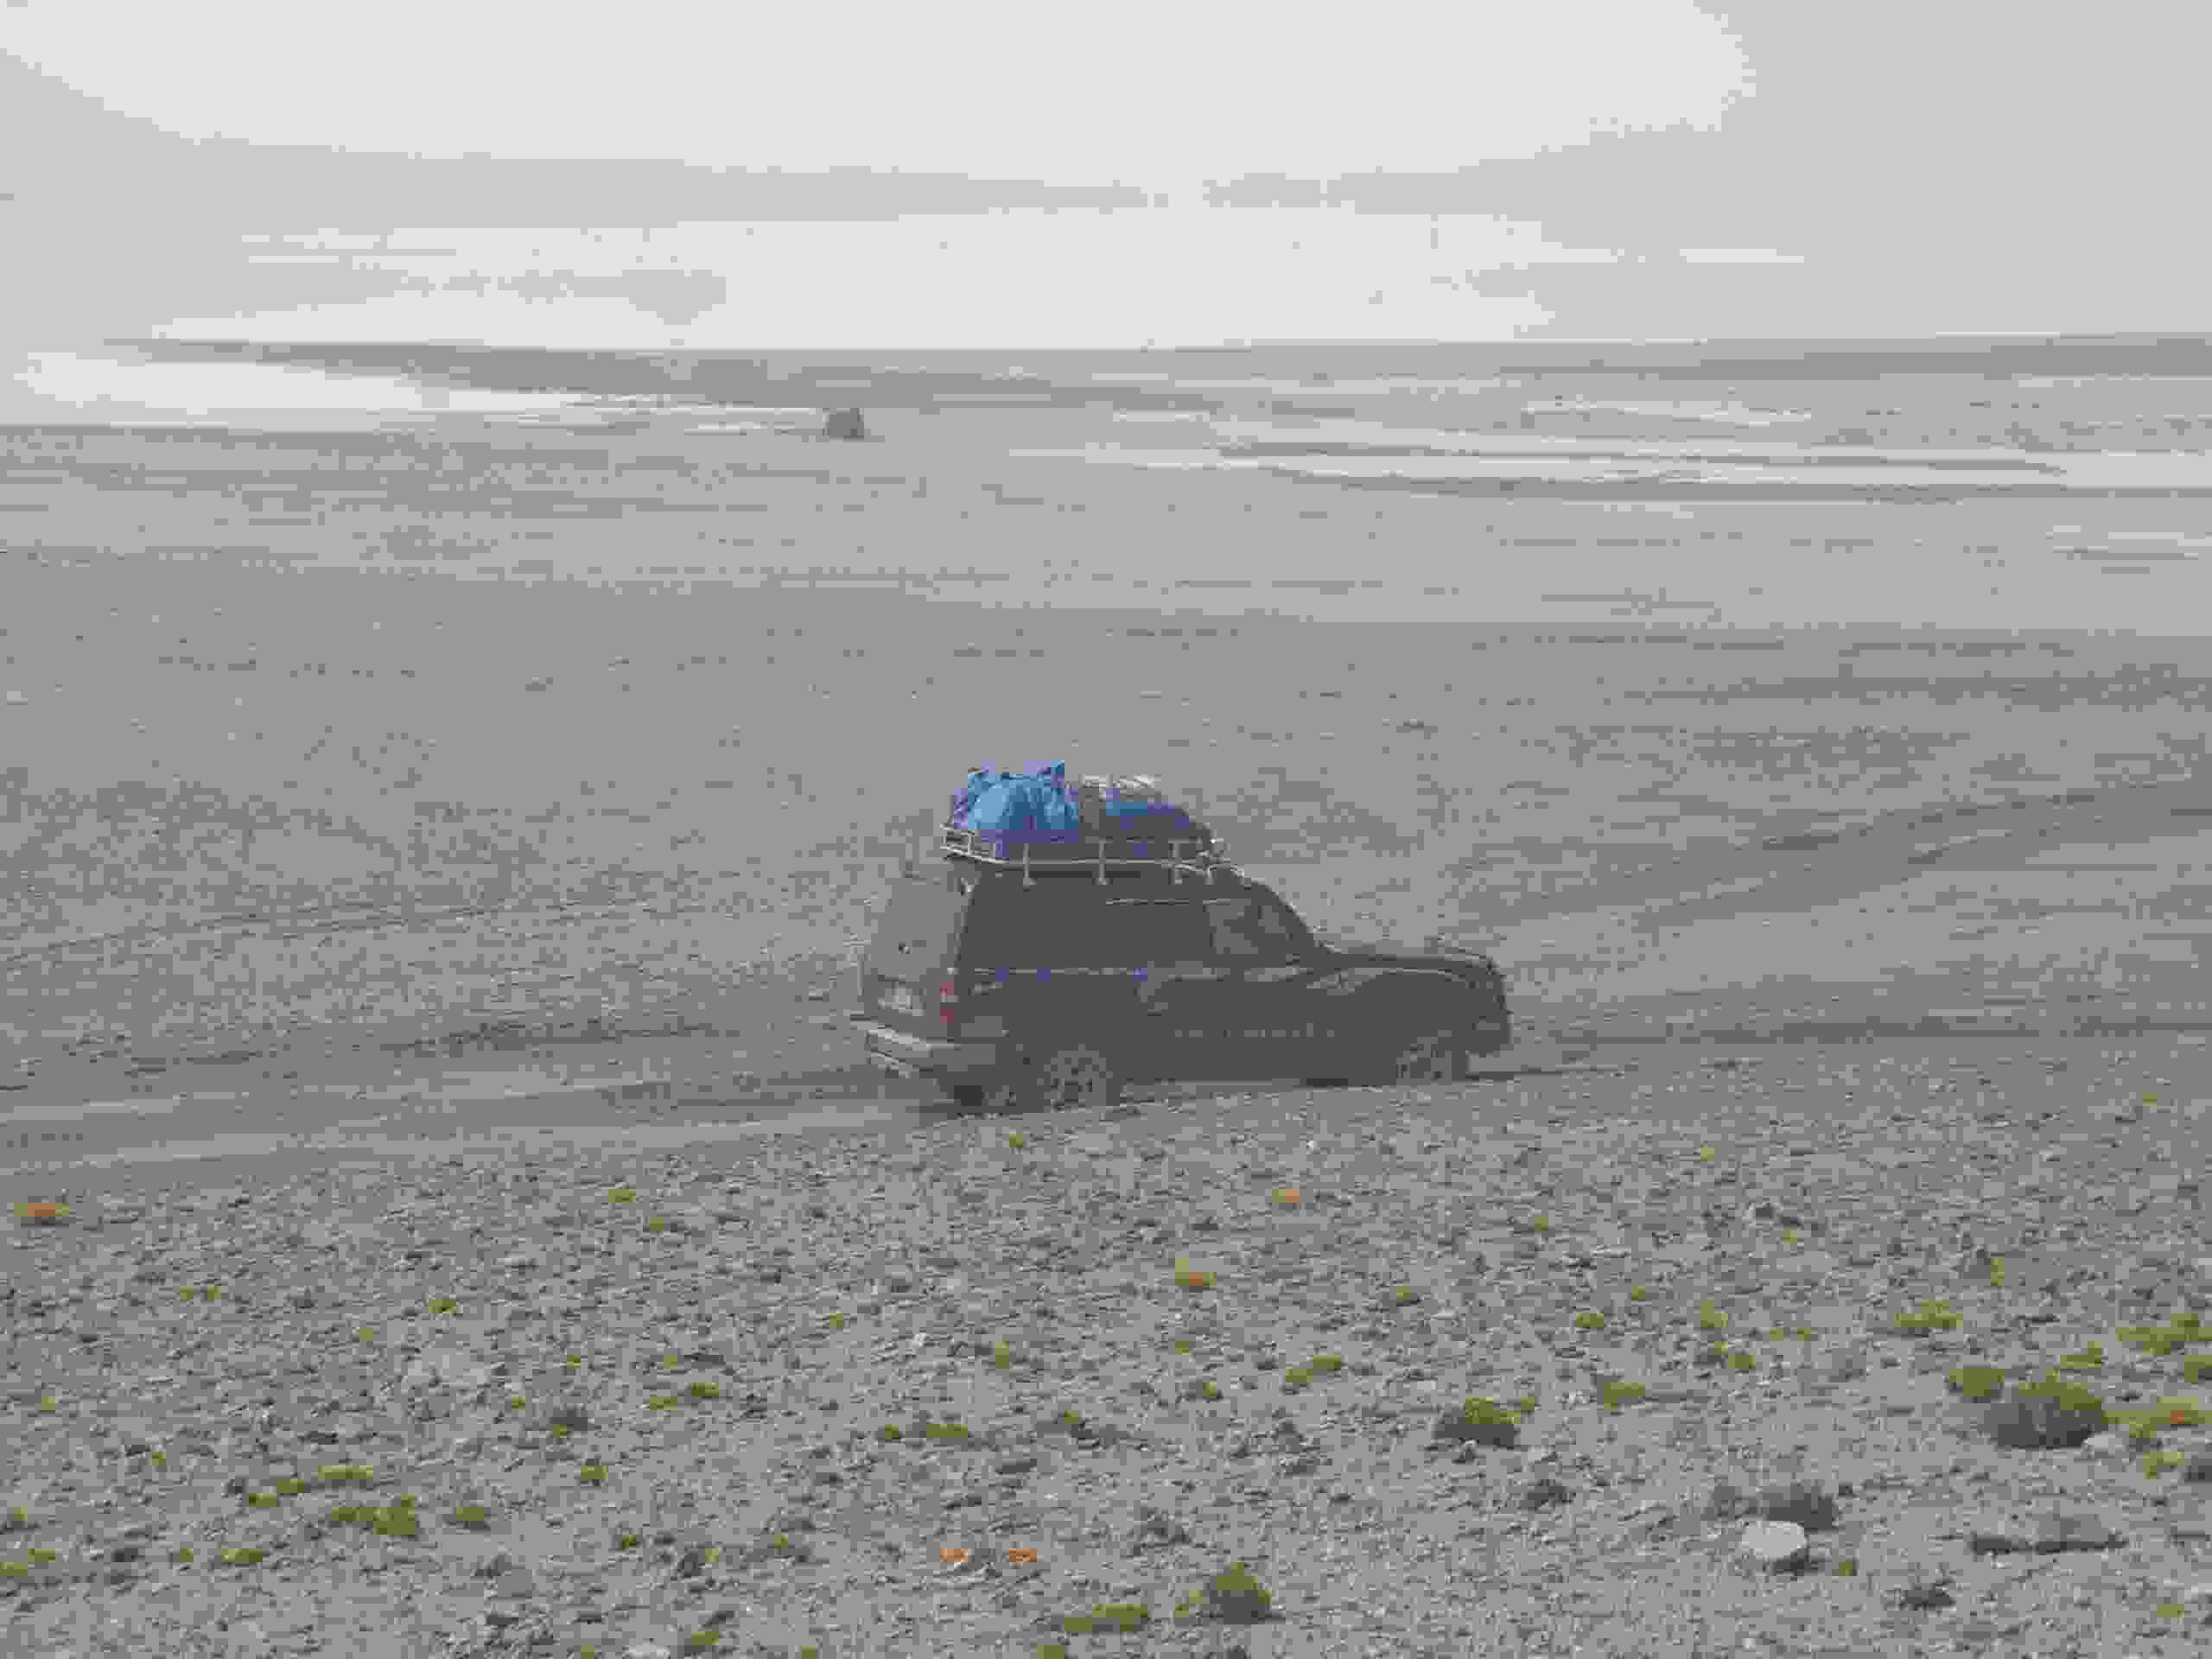
\includegraphics[width=\mywidth]{../wp-content/uploads/2015/04/wpid-wp-1427984048275.jpg} \end{center}

\pagebreak
 Ensuite beau temps, vent dans le dos, piste roulante et paysages magnifiques : le Sud Lipez s'annonce bien !
\begin{center} 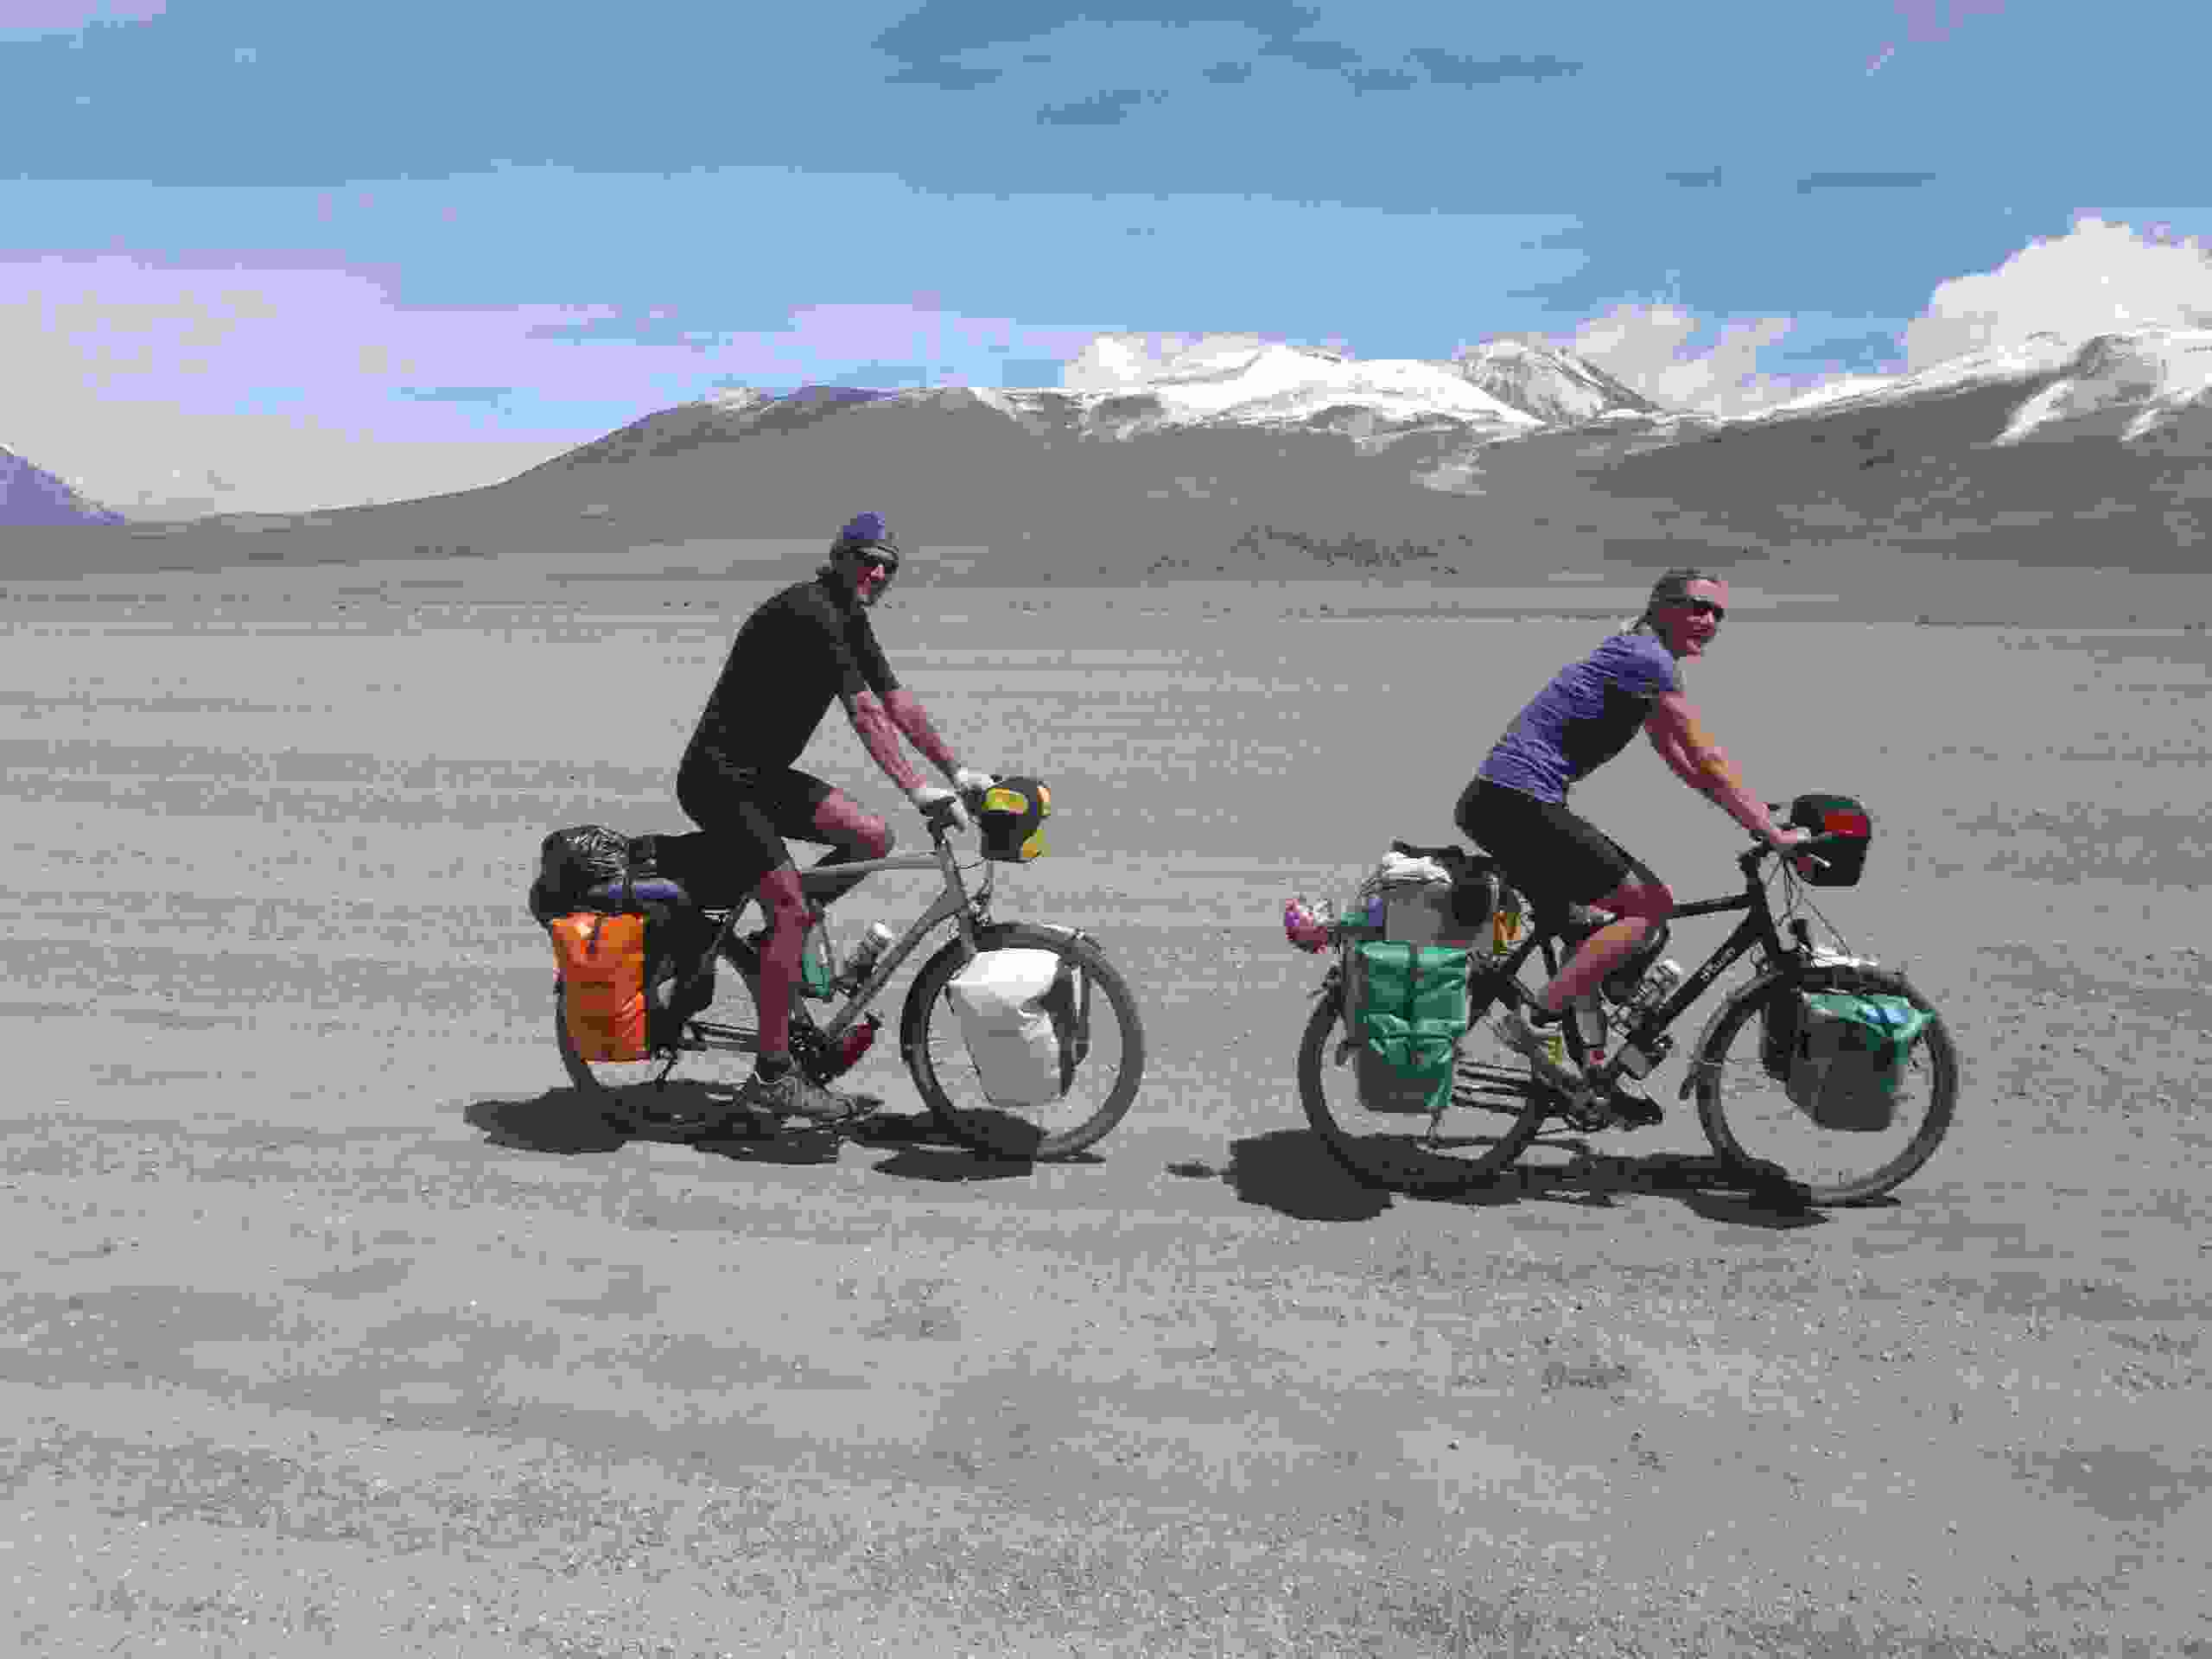
\includegraphics[width=\mywidth]{../wp-content/uploads/2015/04/wpid-wp-1427984125510.jpg} \end{center}
\begin{center} 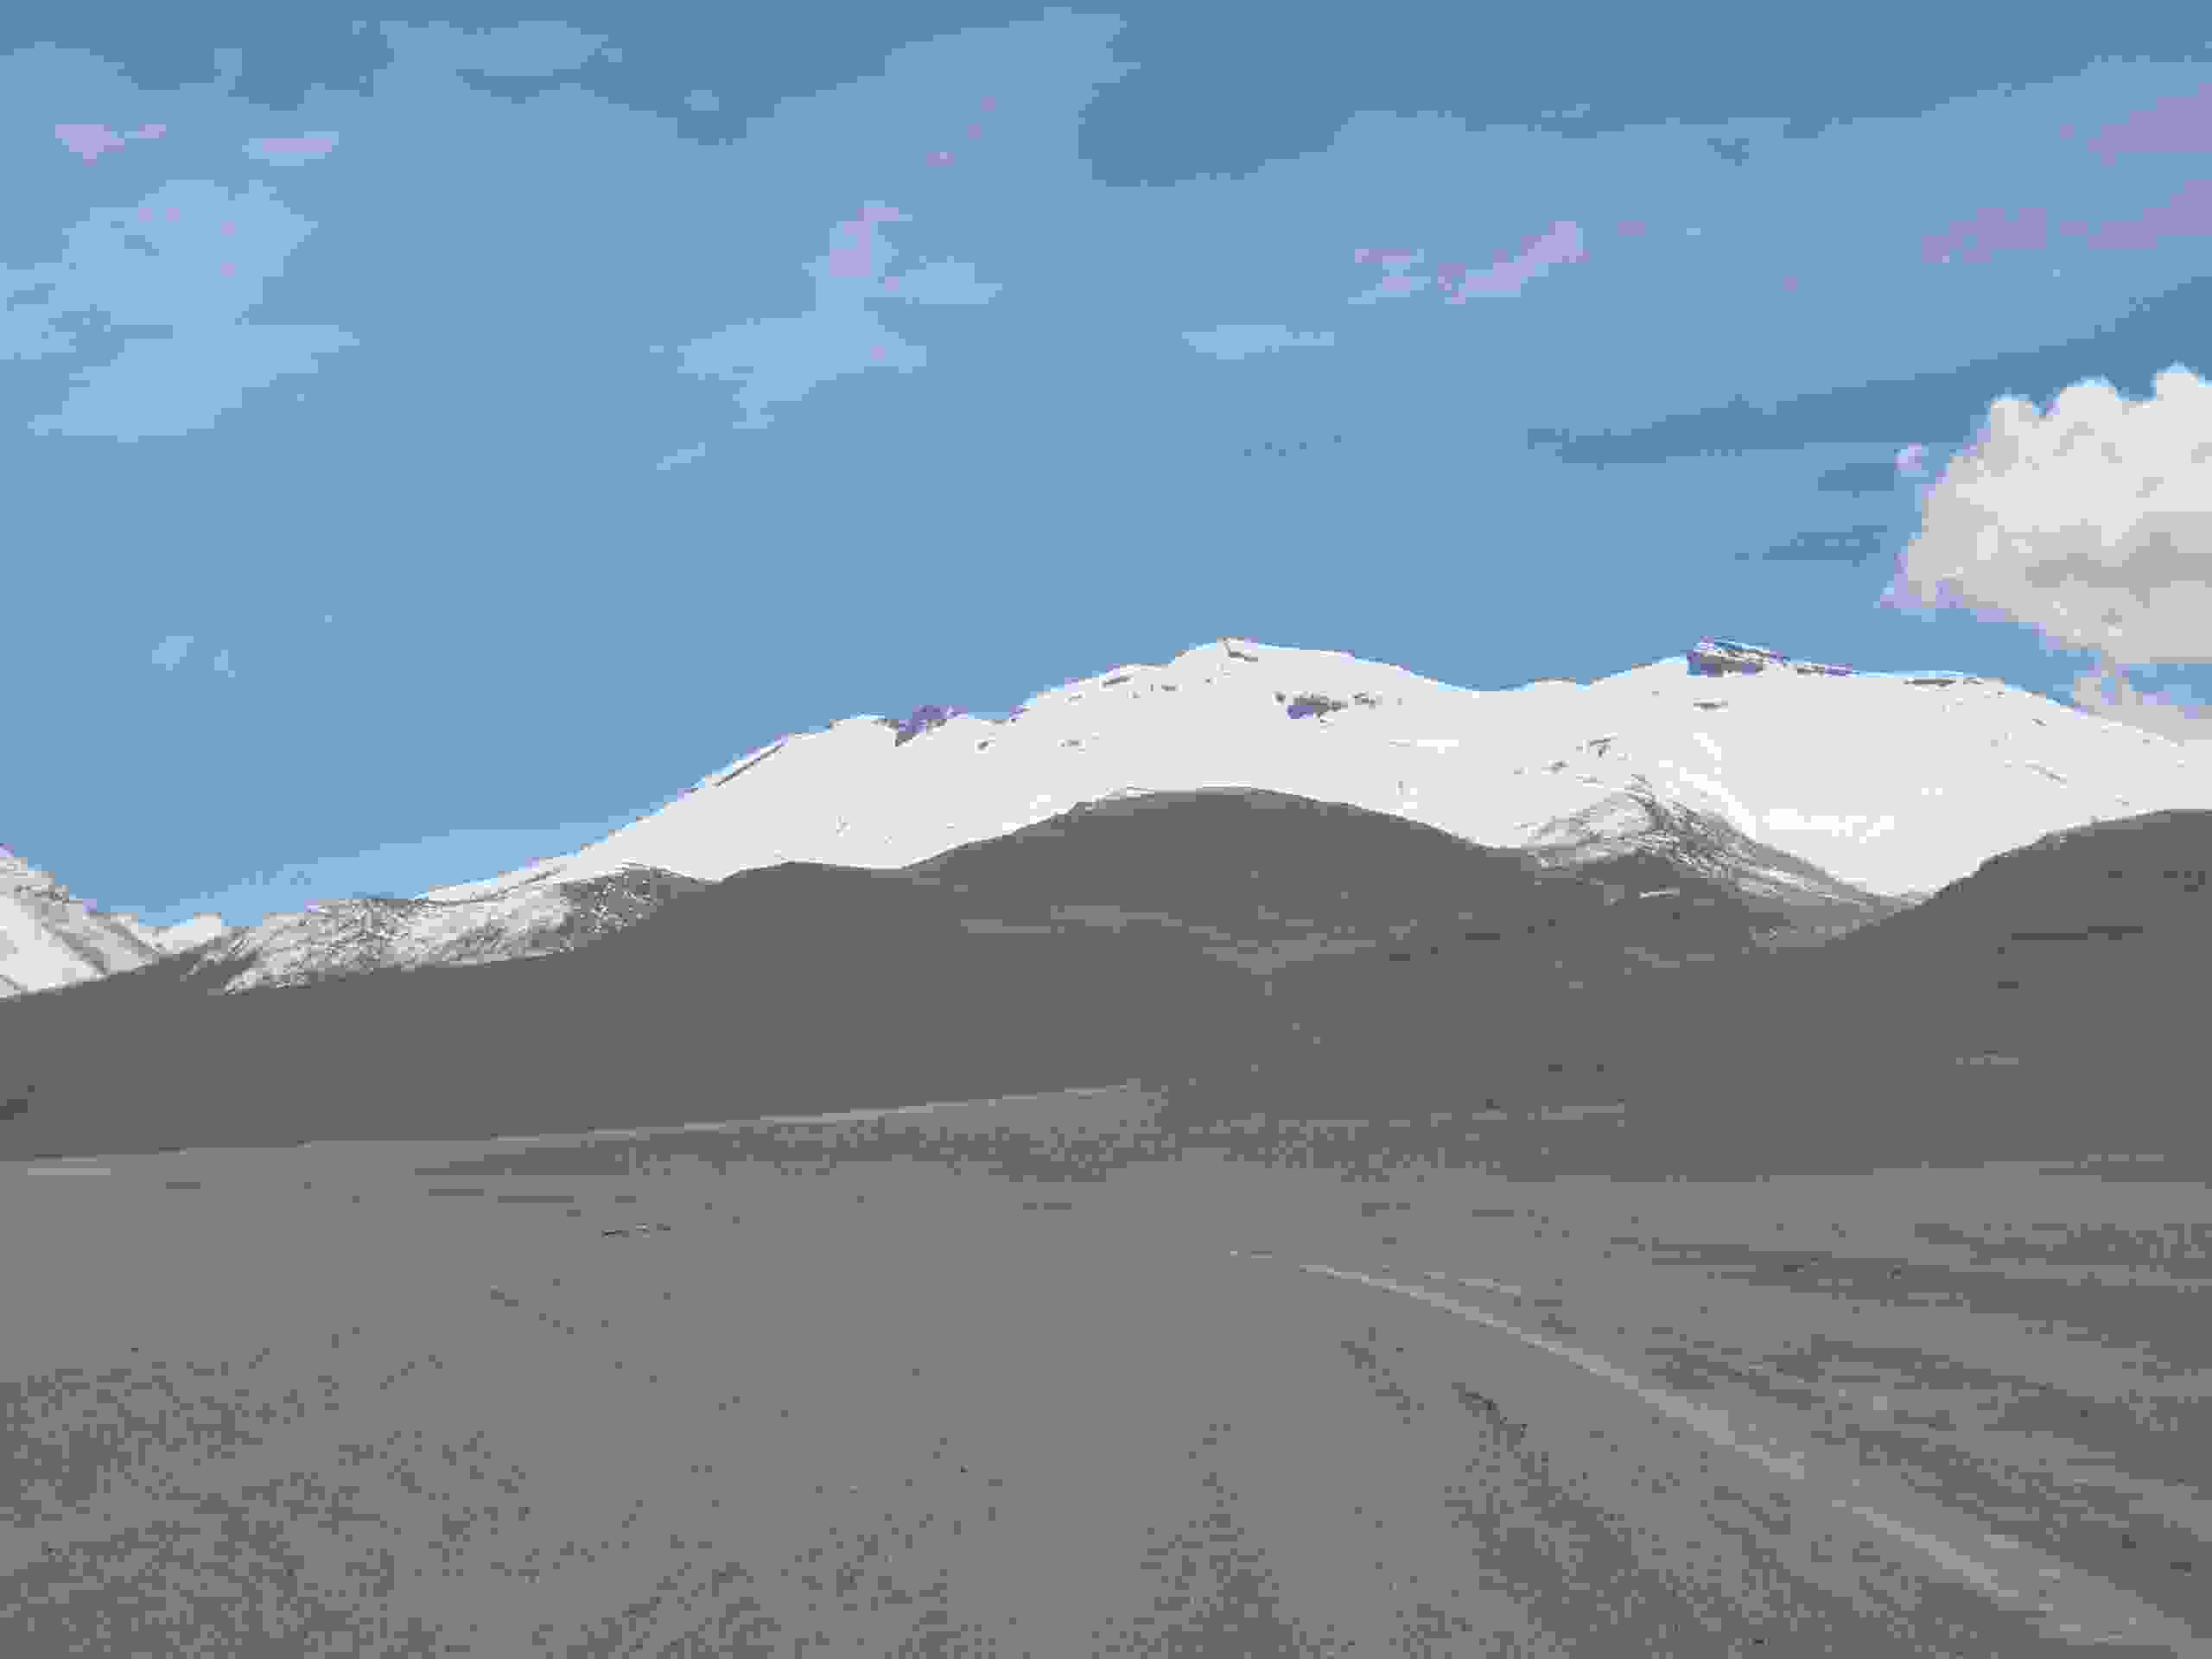
\includegraphics[width=\mywidth]{../wp-content/uploads/2015/04/wpid-wp-1427984230200.jpg} \end{center}
\begin{center} 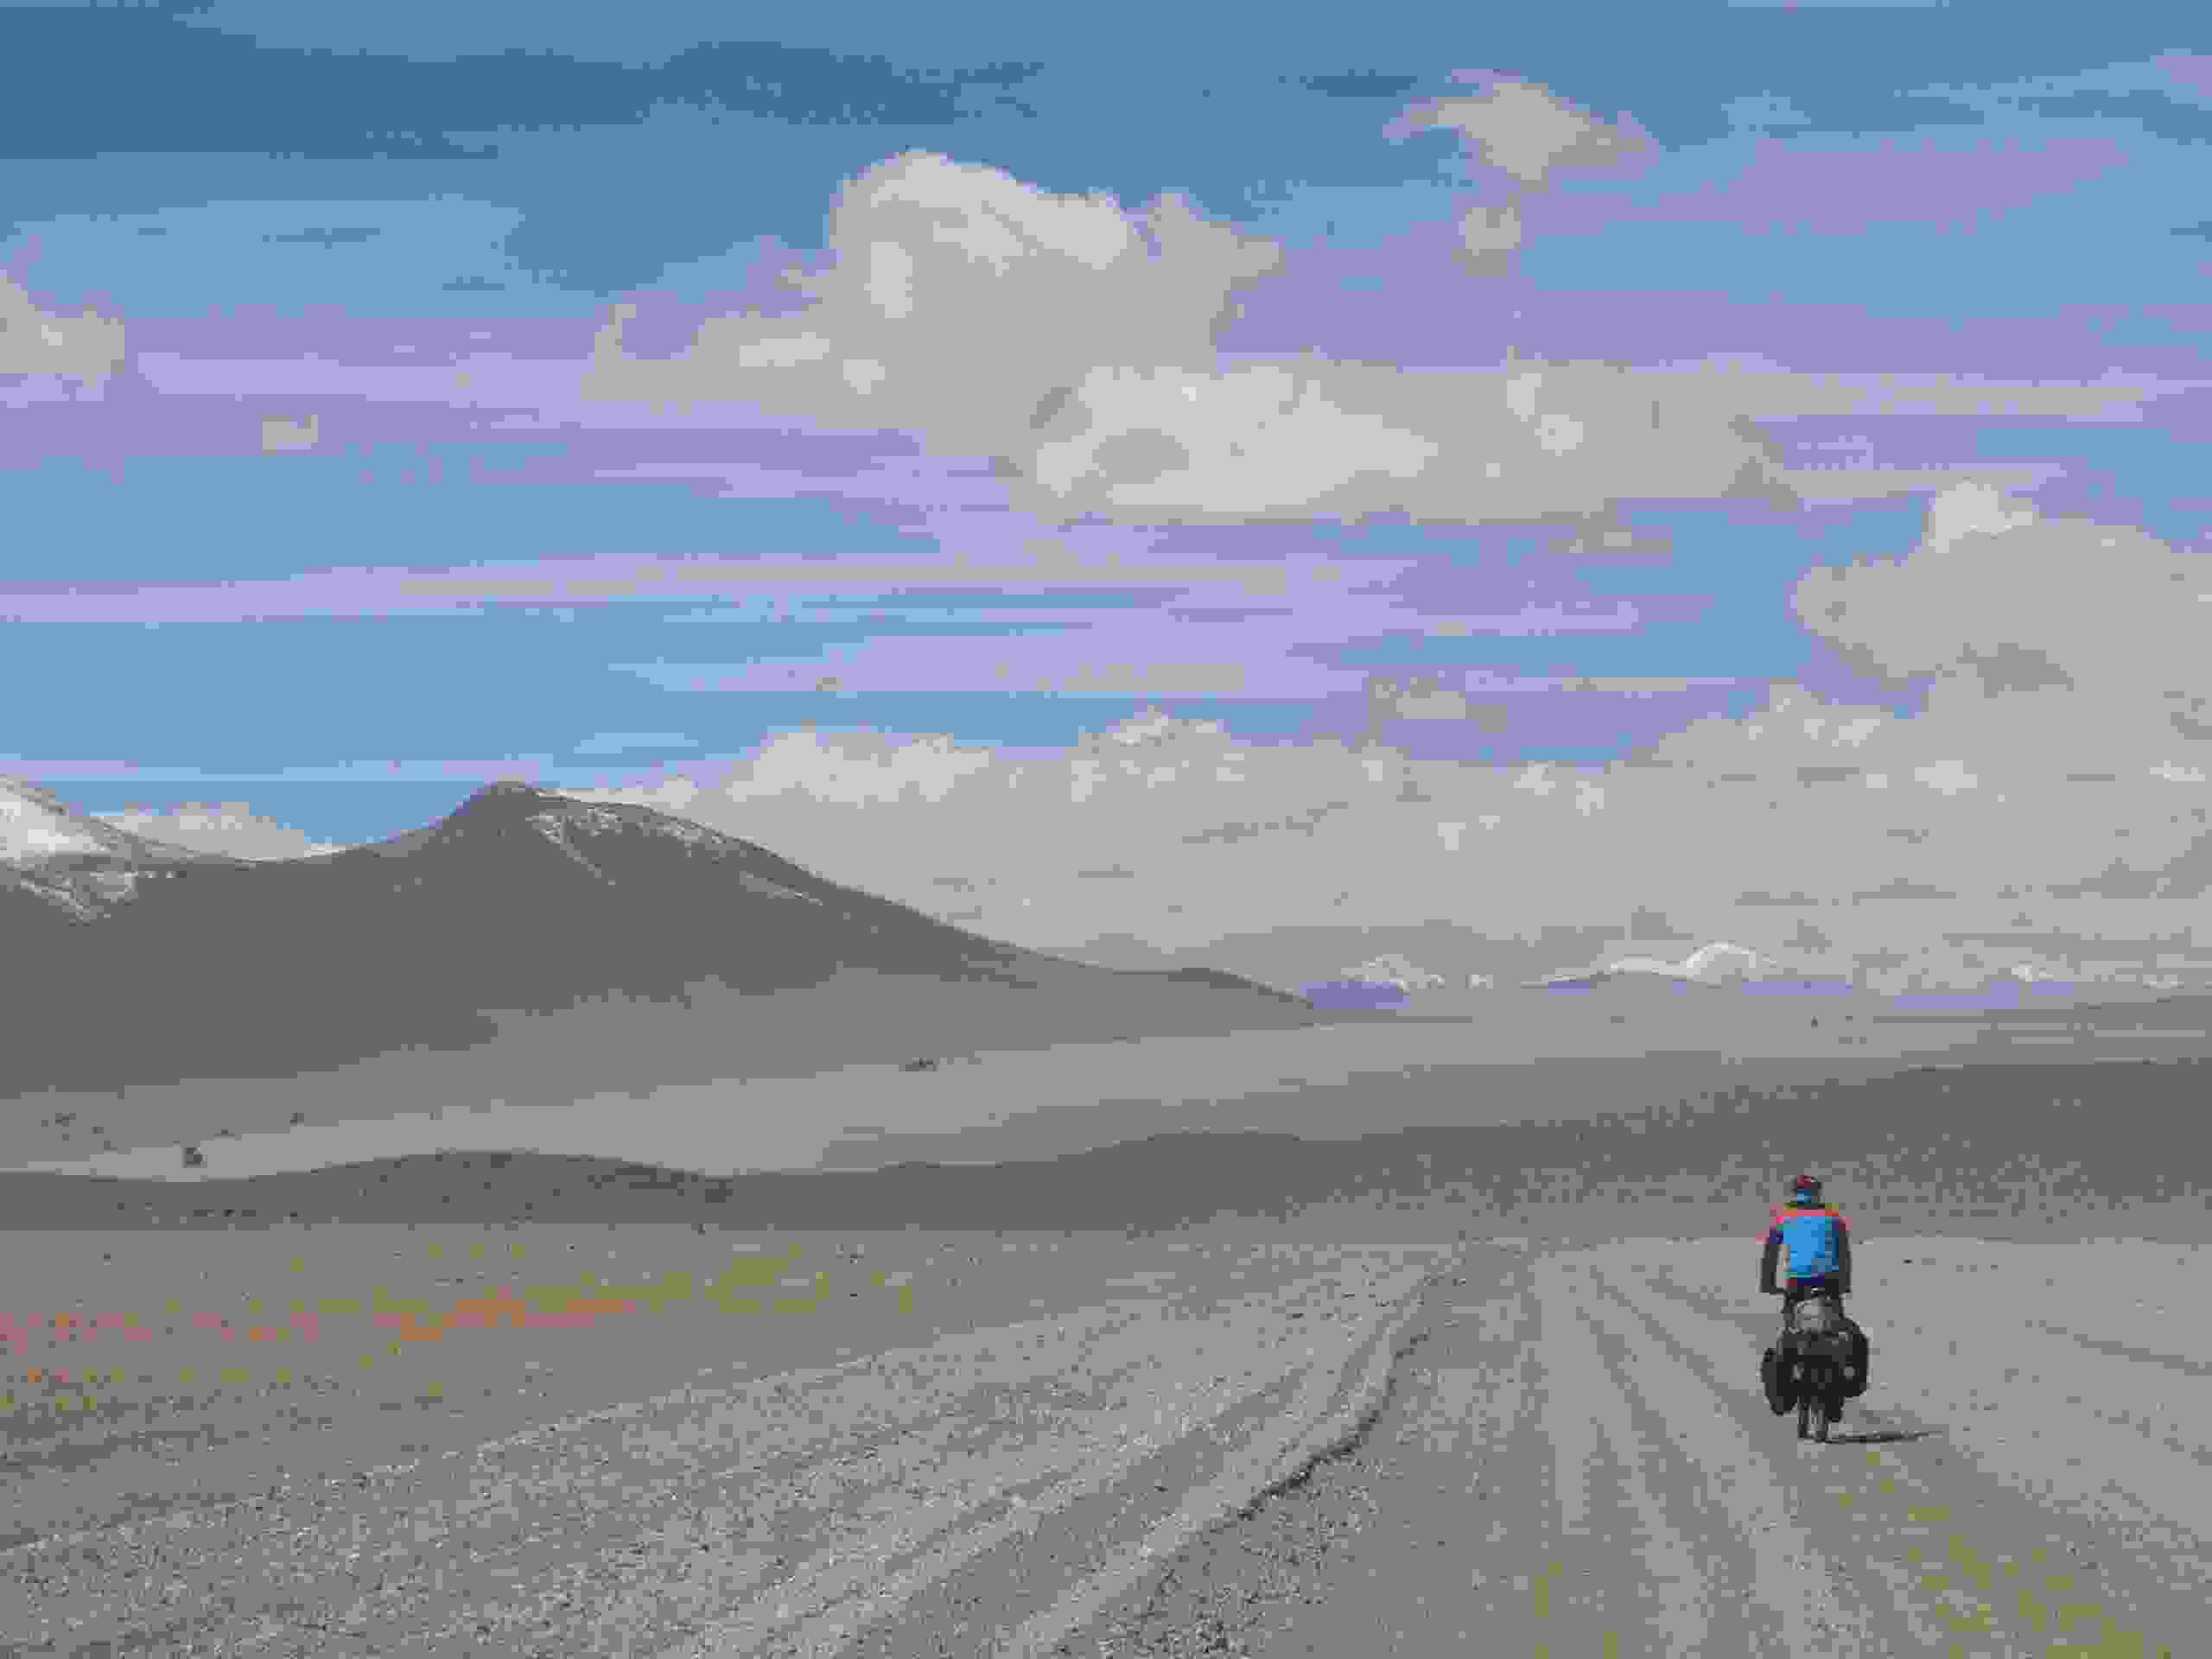
\includegraphics[width=\mywidth]{../wp-content/uploads/2015/04/wpid-wp-1427944069877.jpg} \end{center}
\begin{center} 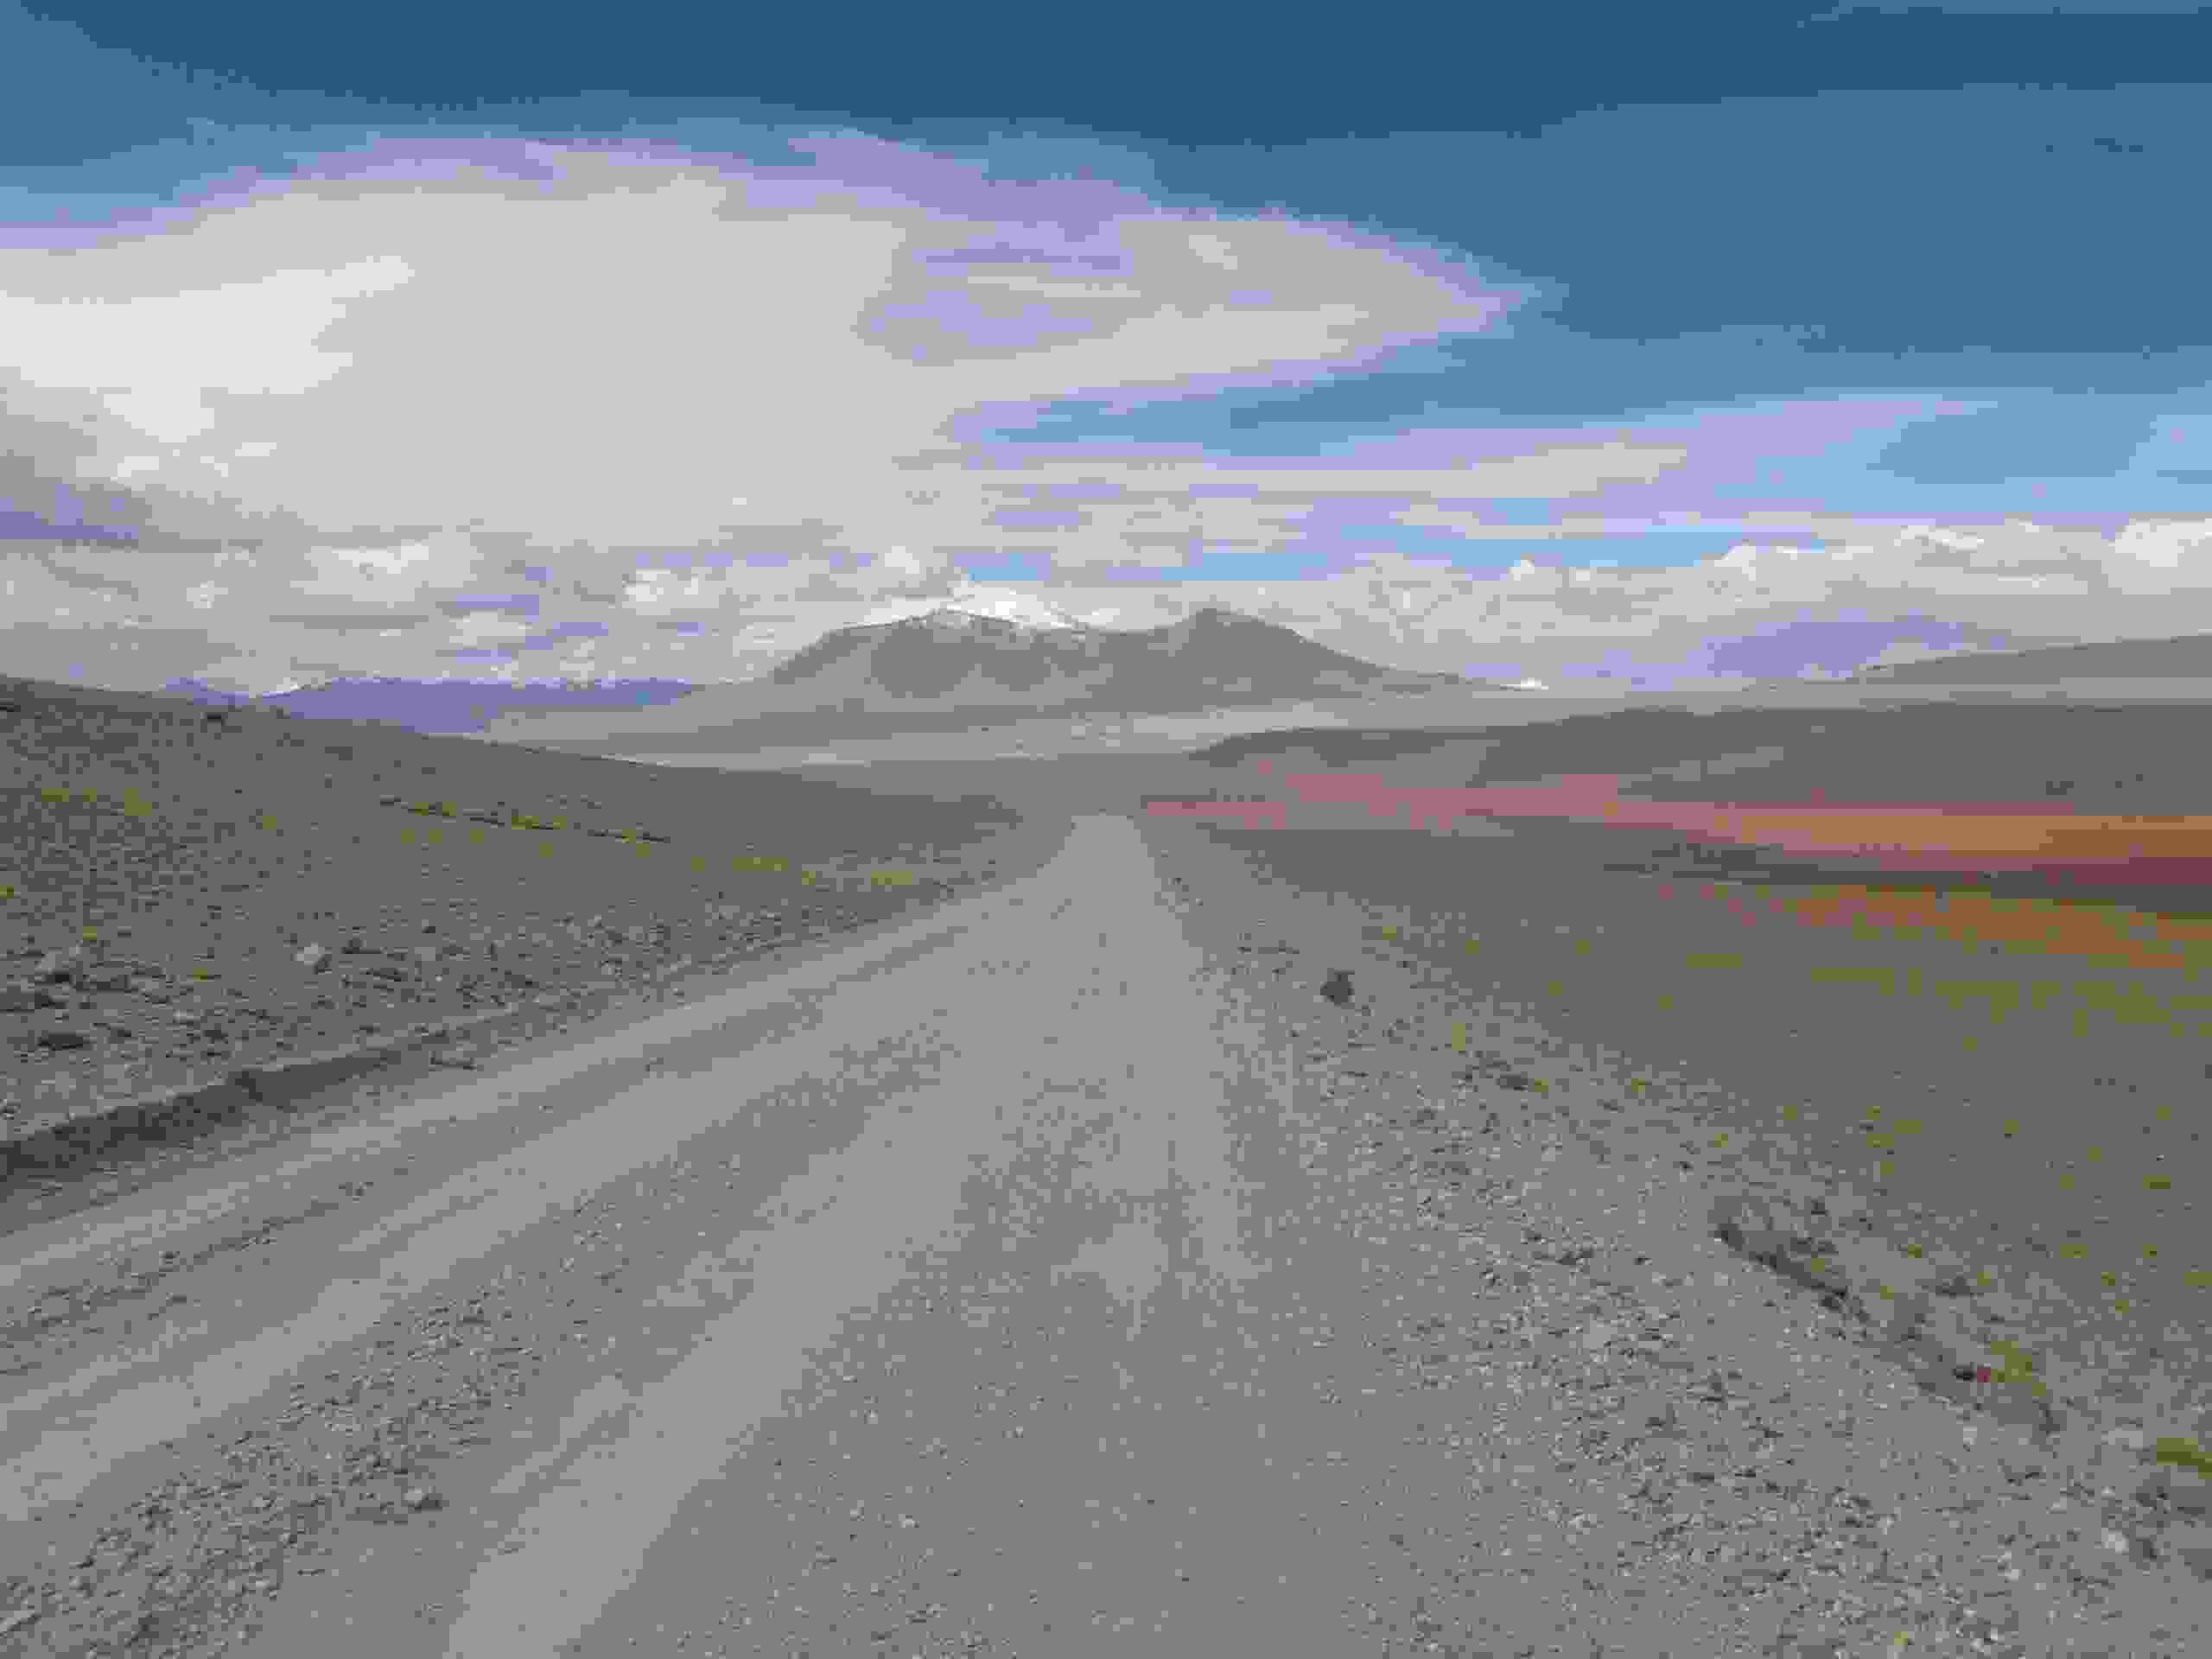
\includegraphics[width=\mywidth]{../wp-content/uploads/2015/04/wpid-wp-1427984180040.jpg} \end{center}

\pagebreak
 On passe devant le Desierto de Dali.
\begin{center} 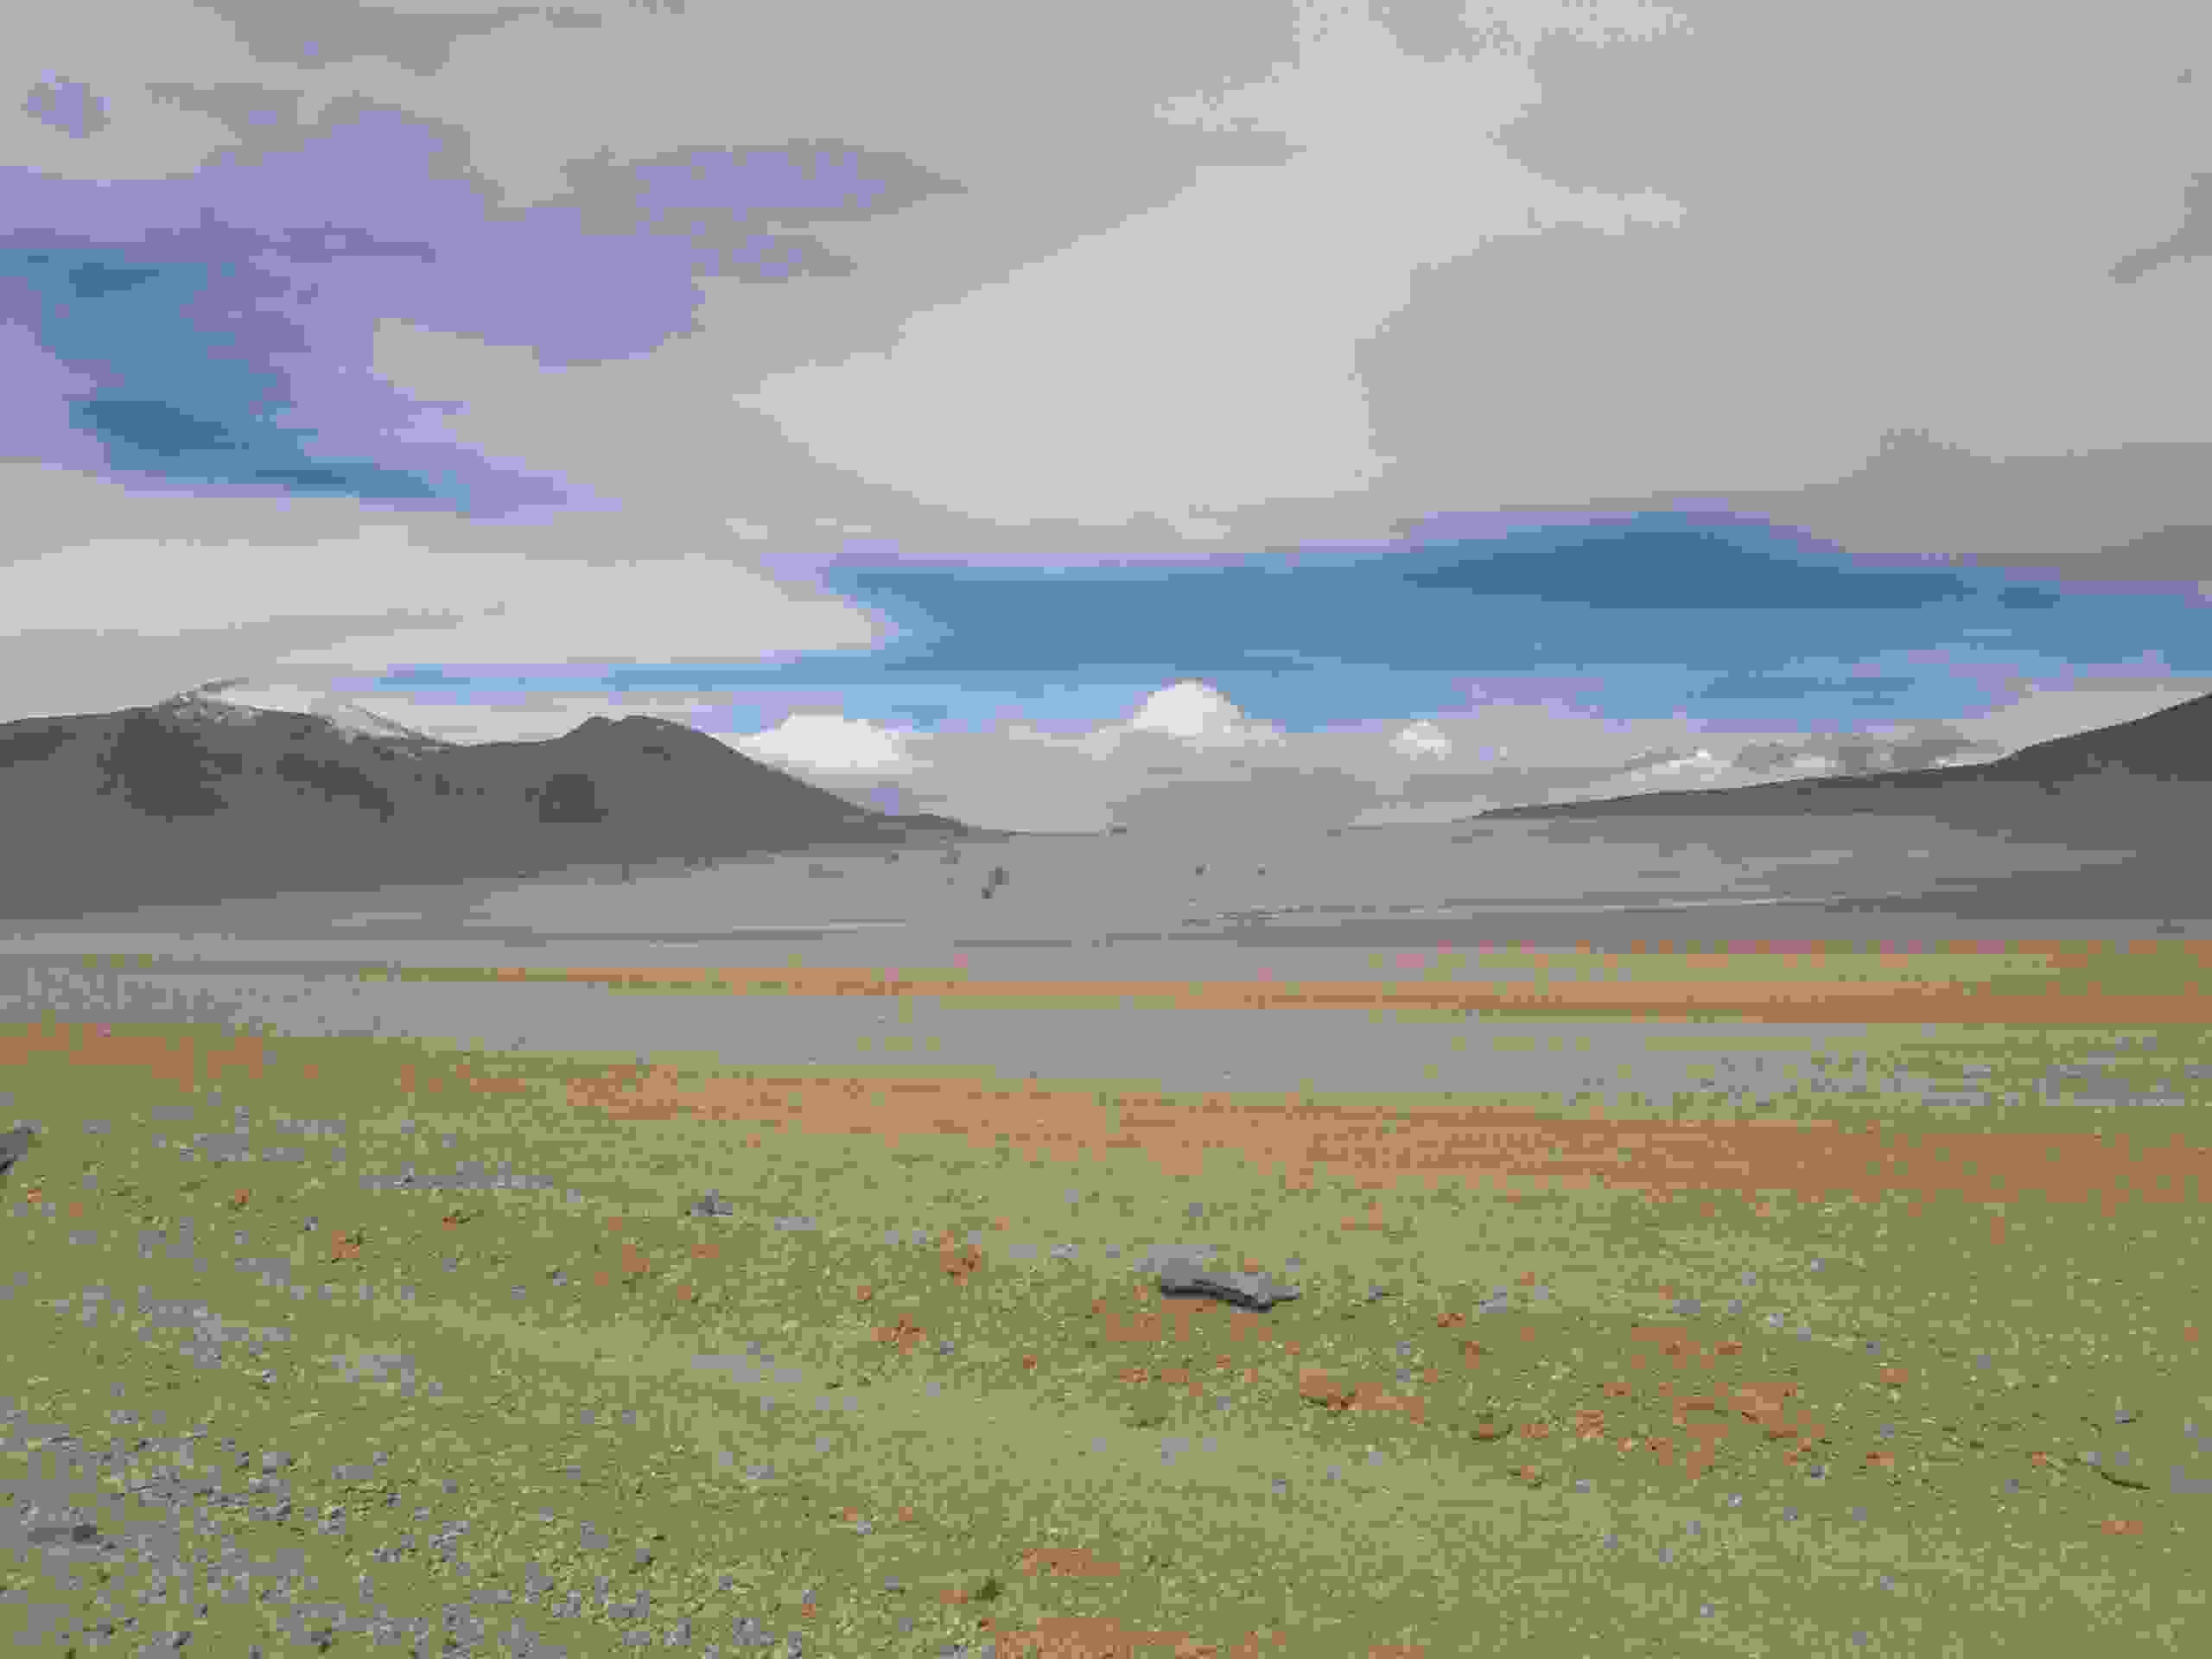
\includegraphics[width=\mywidth]{../wp-content/uploads/2015/04/wpid-wp-1427984489619.jpg} \end{center}

 Piscine d'eau chaude devant la Laguna Chalviri pour terminer la journée.
\begin{center} 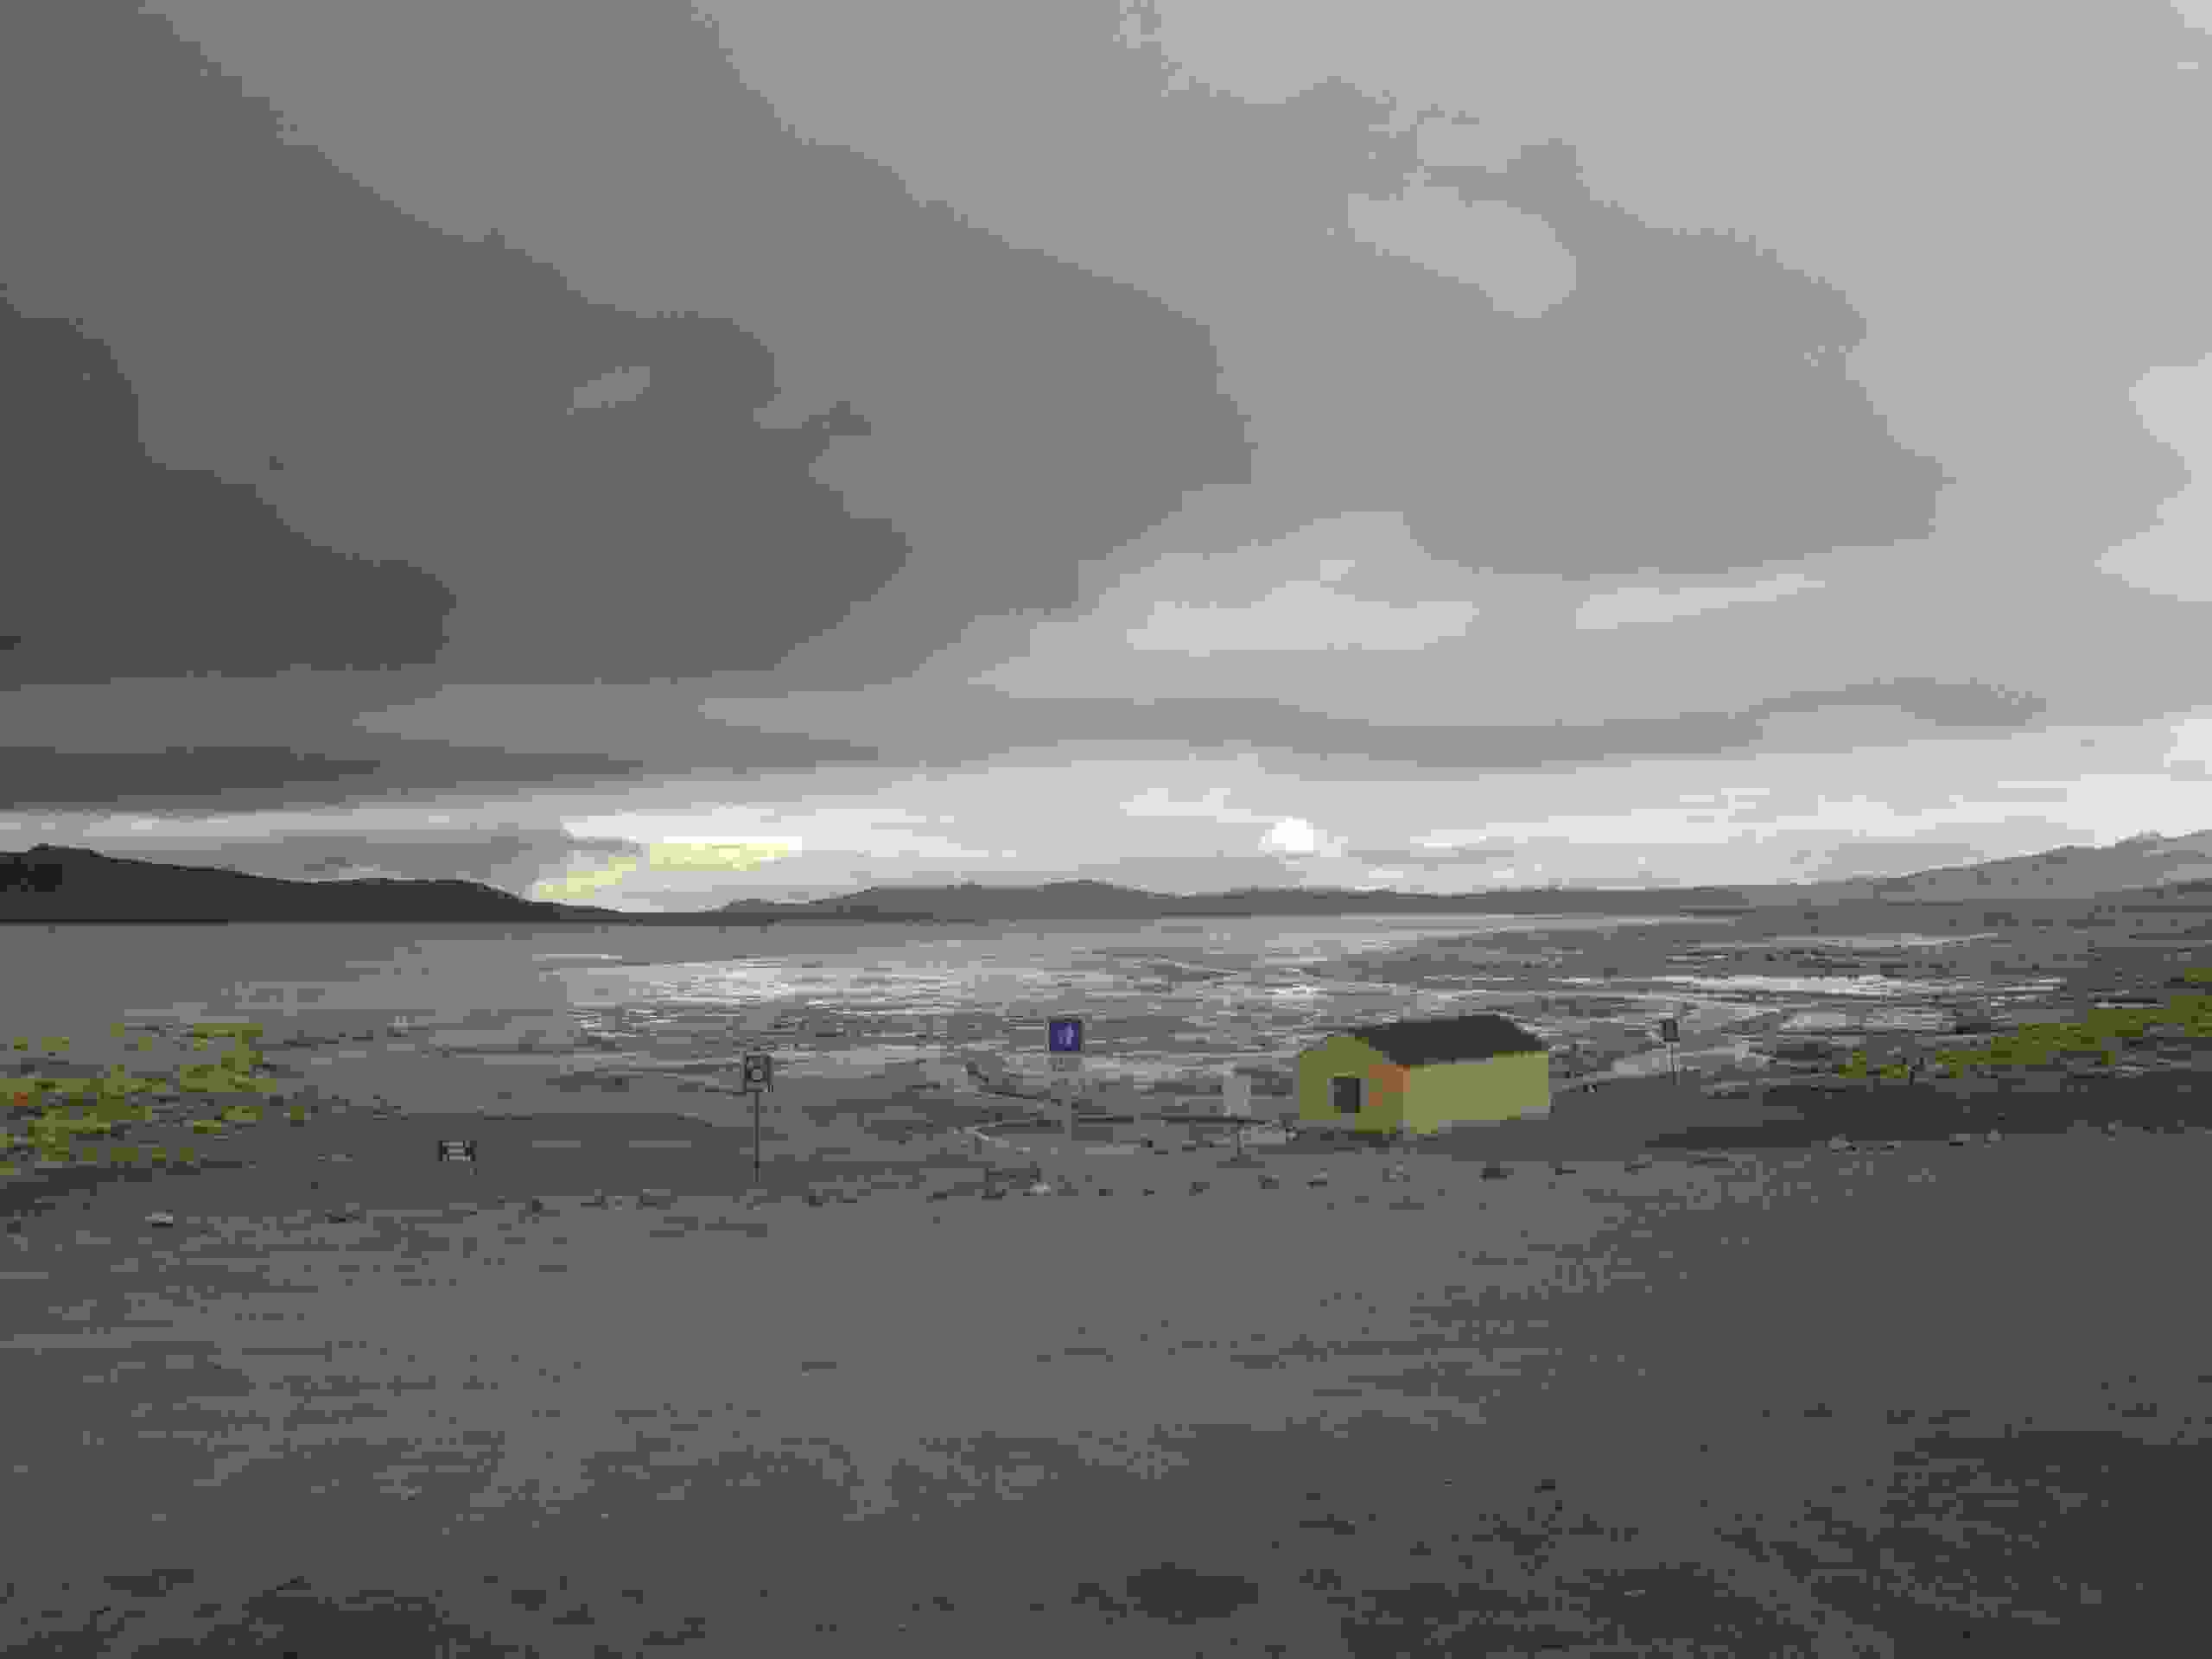
\includegraphics[width=\mywidth]{../wp-content/uploads/2015/04/wpid-wp-1427984540238.jpg} \end{center}
\begin{center} 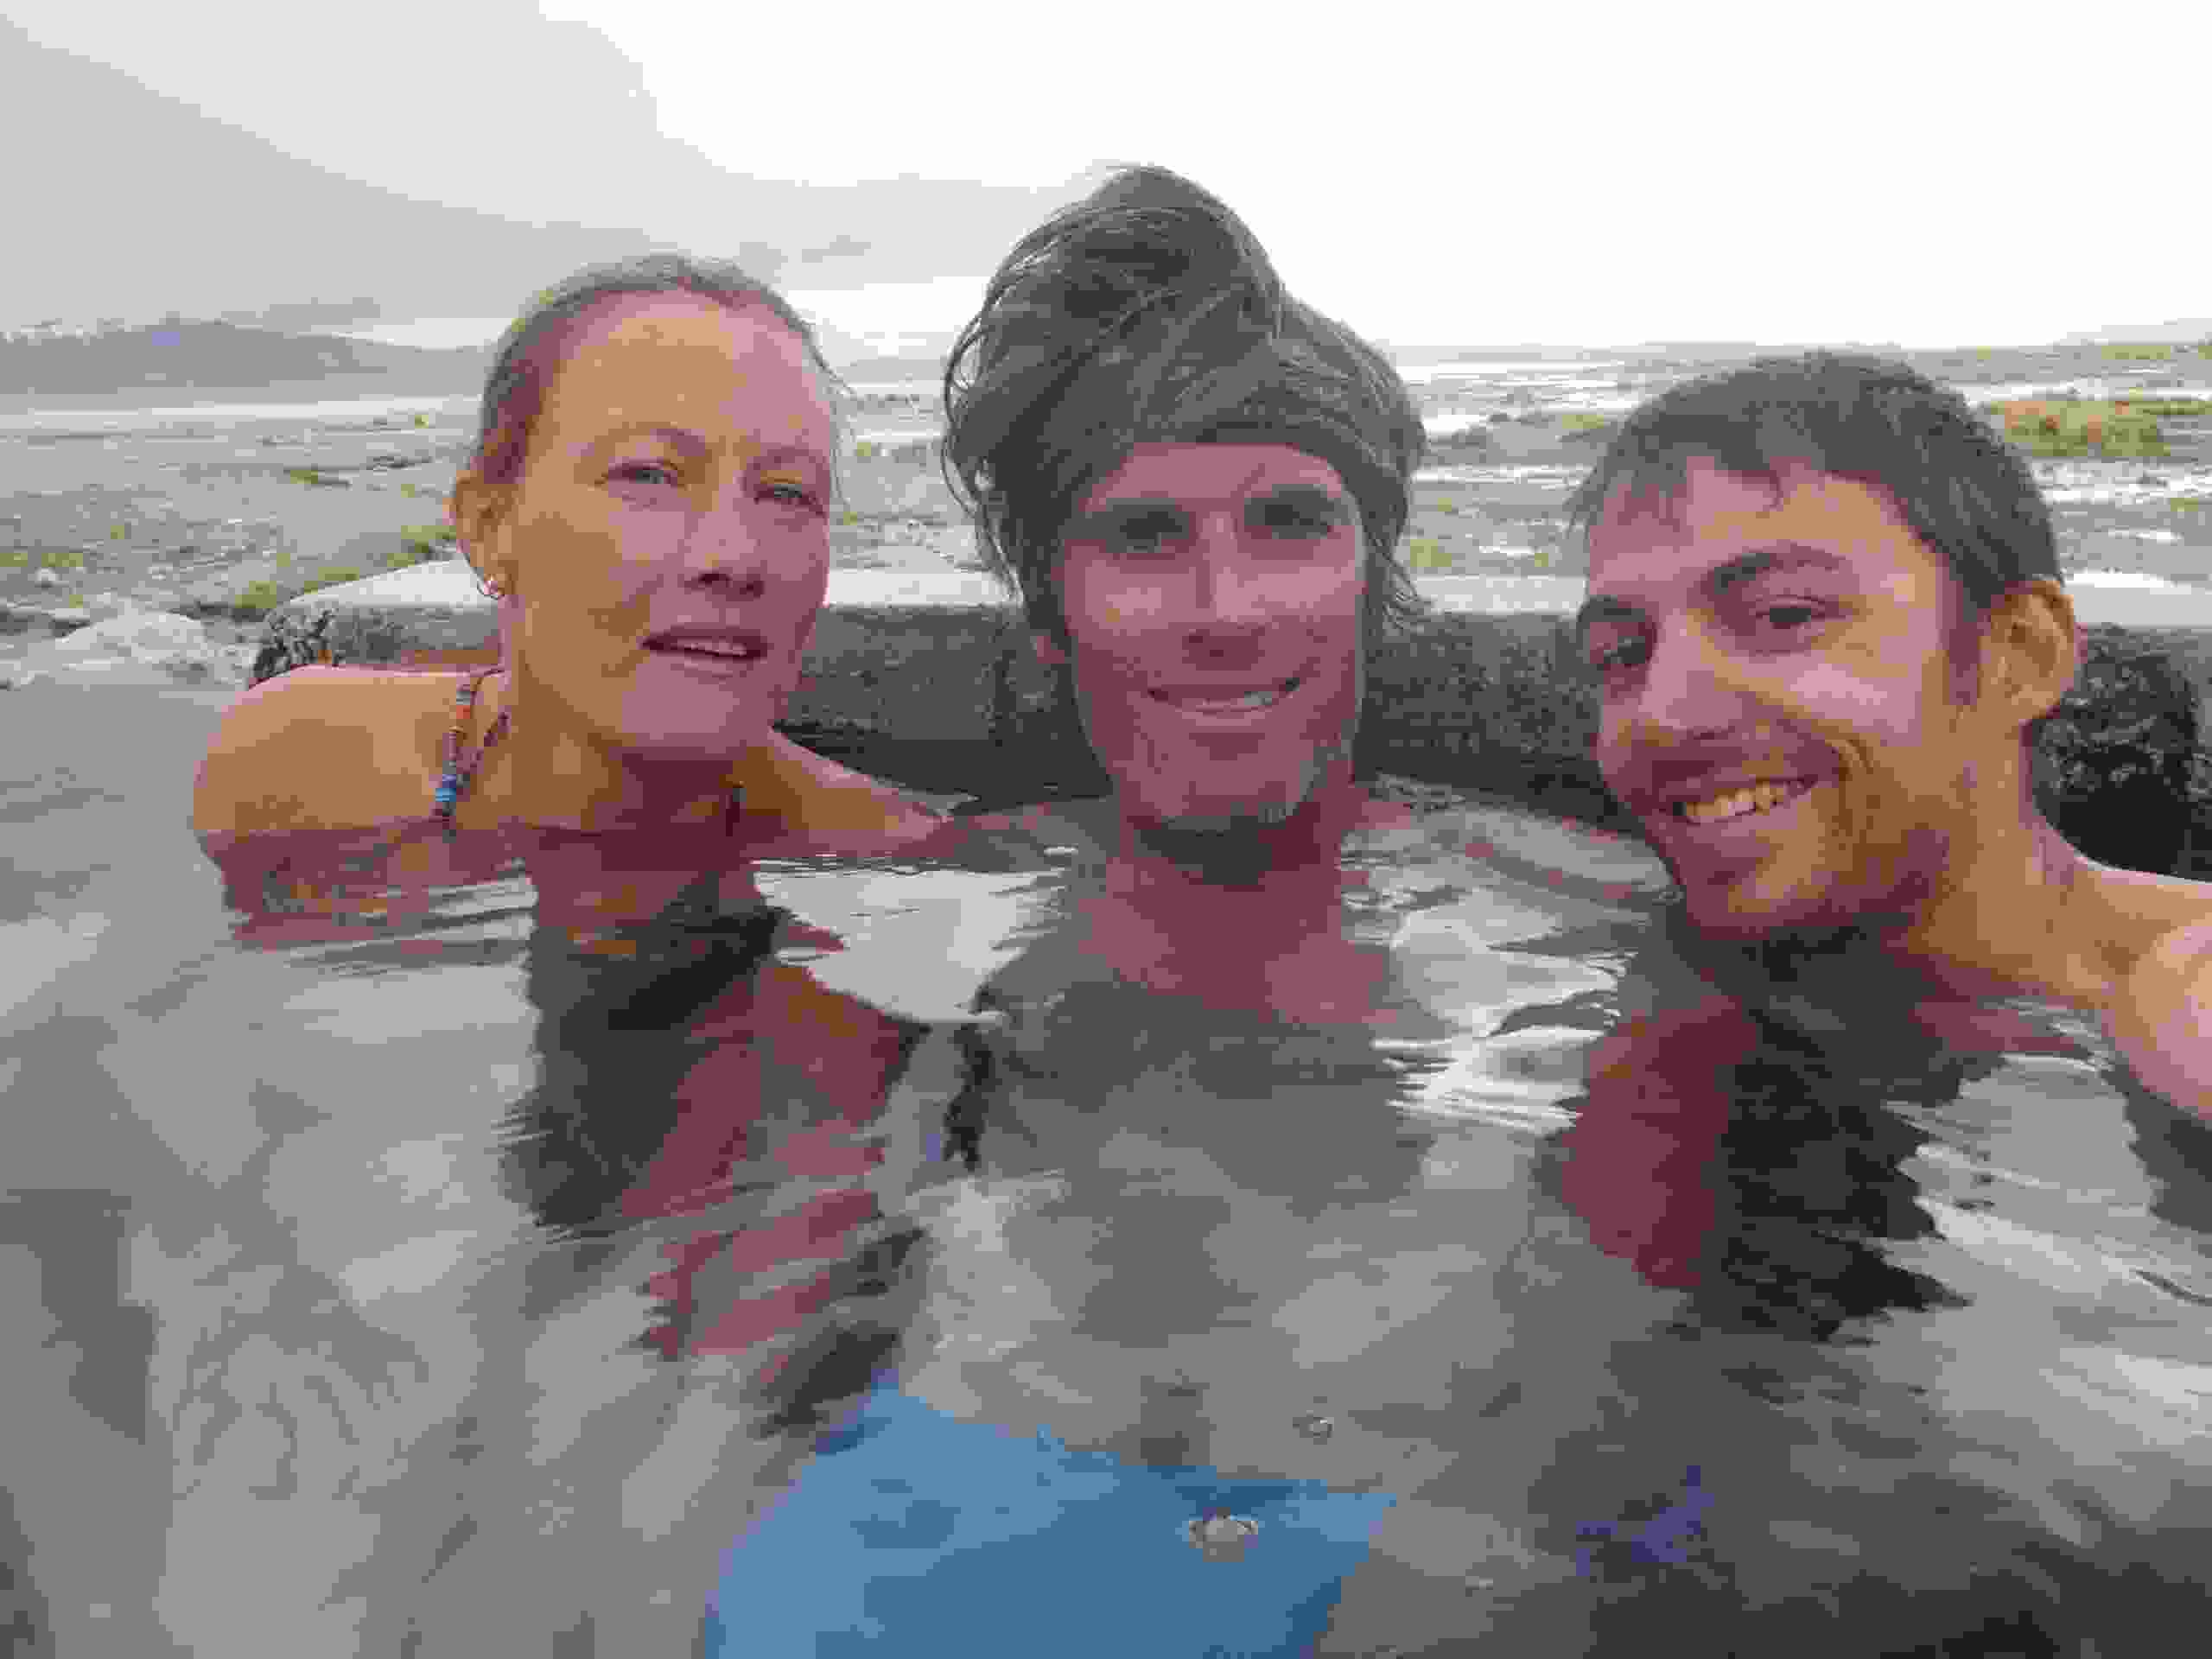
\includegraphics[width=\mywidth]{../wp-content/uploads/2015/04/wpid-wp-1427984554621.jpg} \end{center}

 On passe la nuit dans la salle à manger d'un restaurant.
\begin{center} 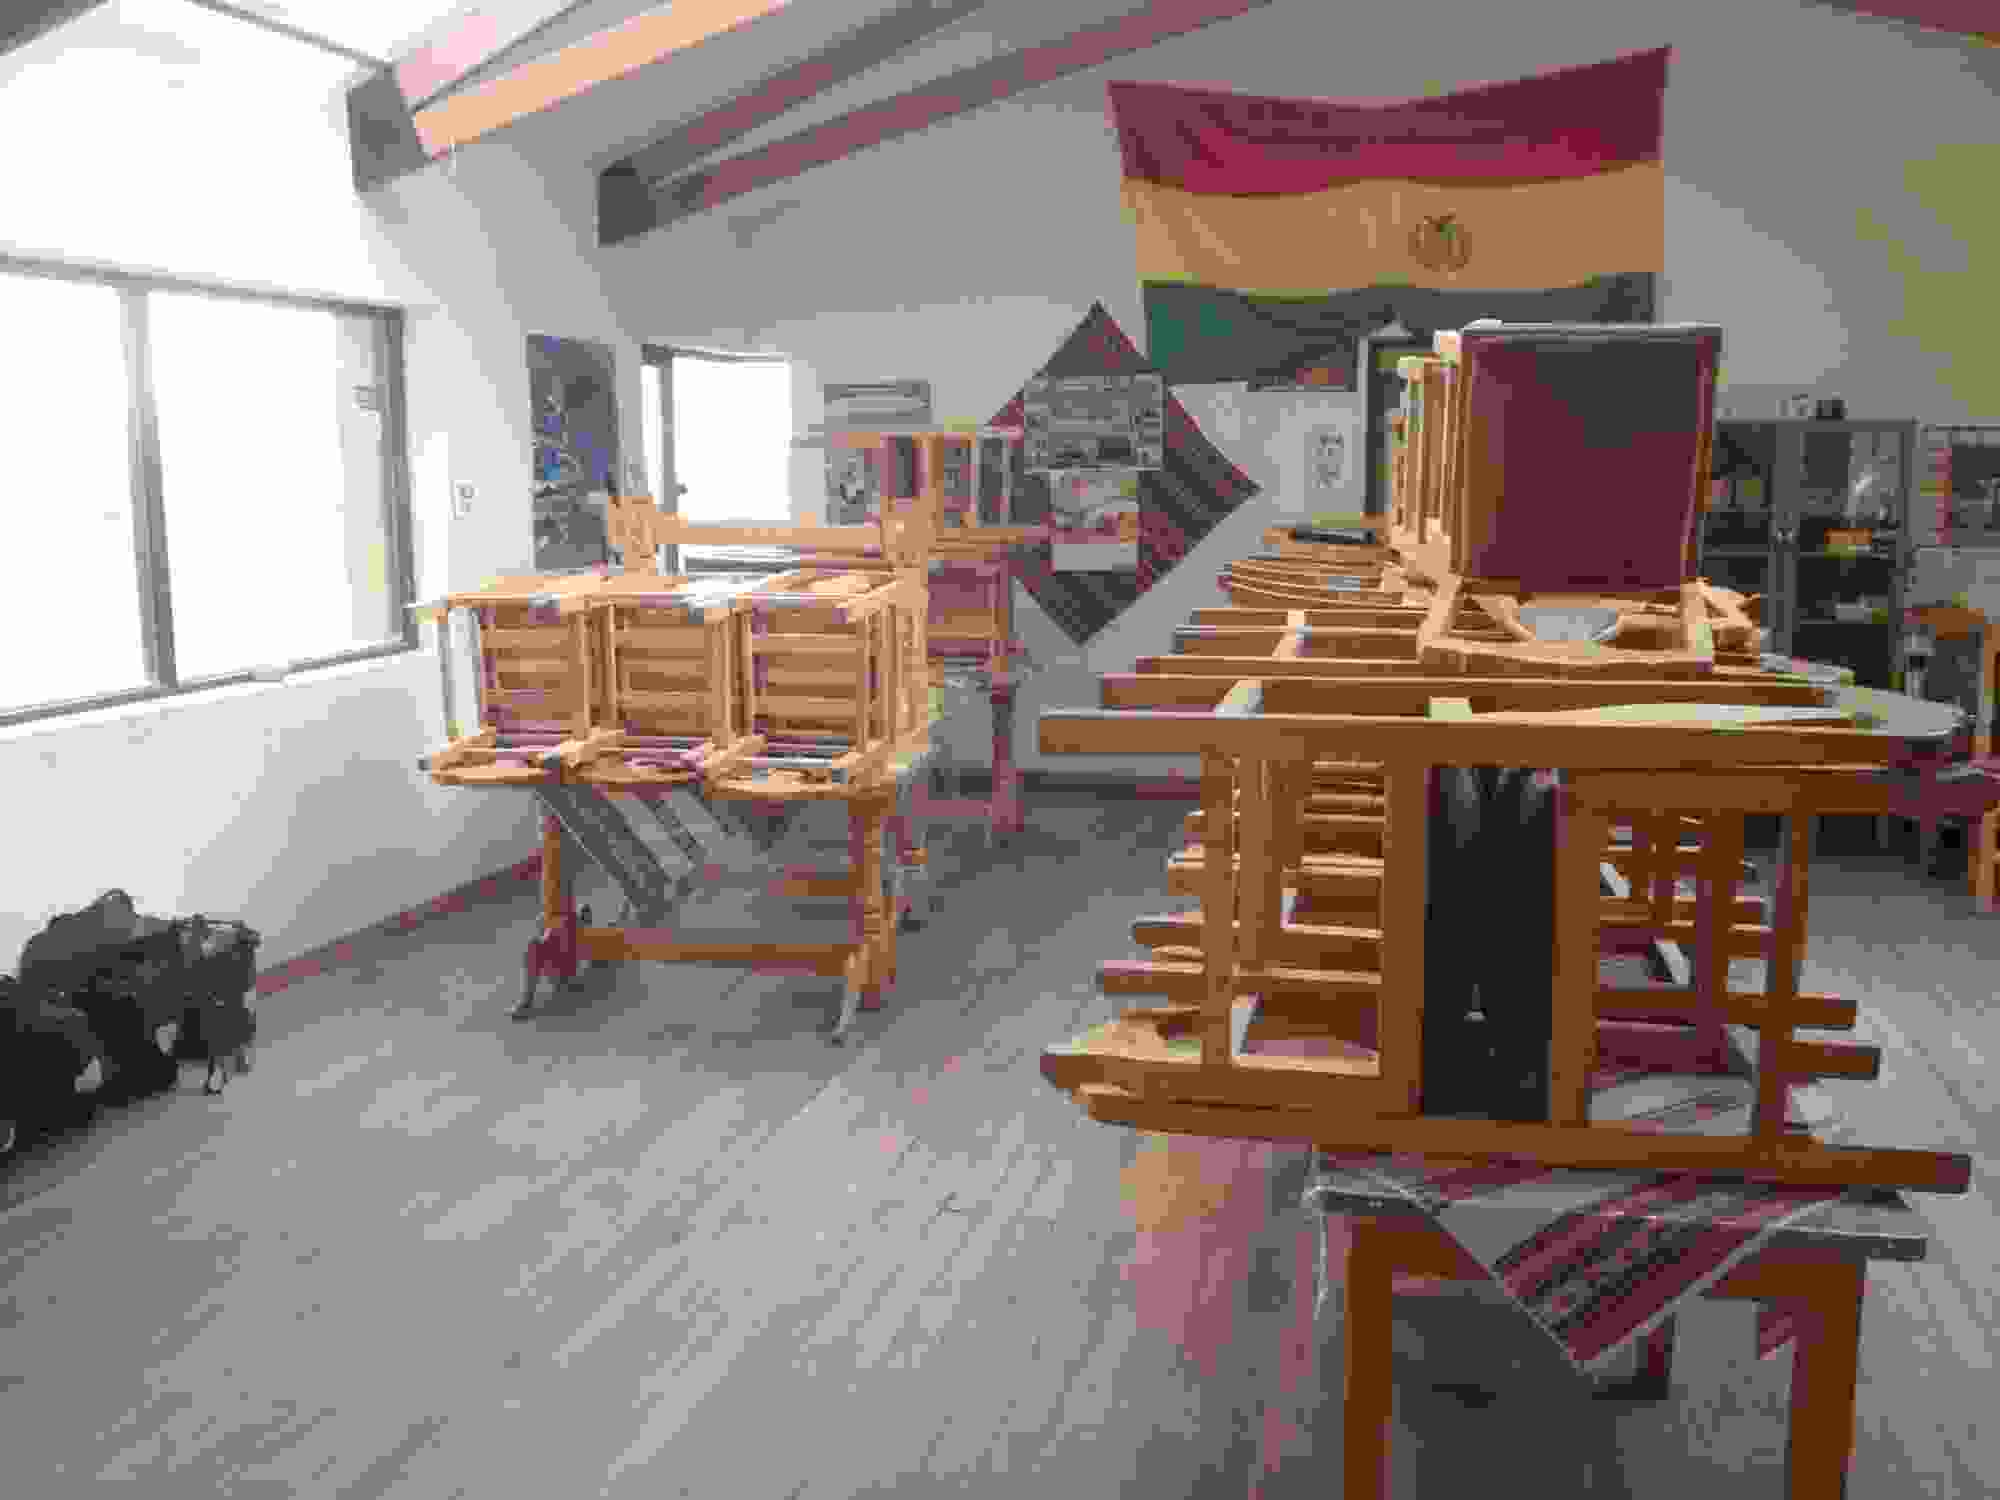
\includegraphics[width=\mywidth]{../wp-content/uploads/2015/04/wpid-wp-1427988917183.jpg} \end{center}

\pagebreak
\subsection*{3\ieme\ jour} 
 Lever à 6h pour laisser la place aux touristes en jeep pour le petit déjeuner.
\begin{center} 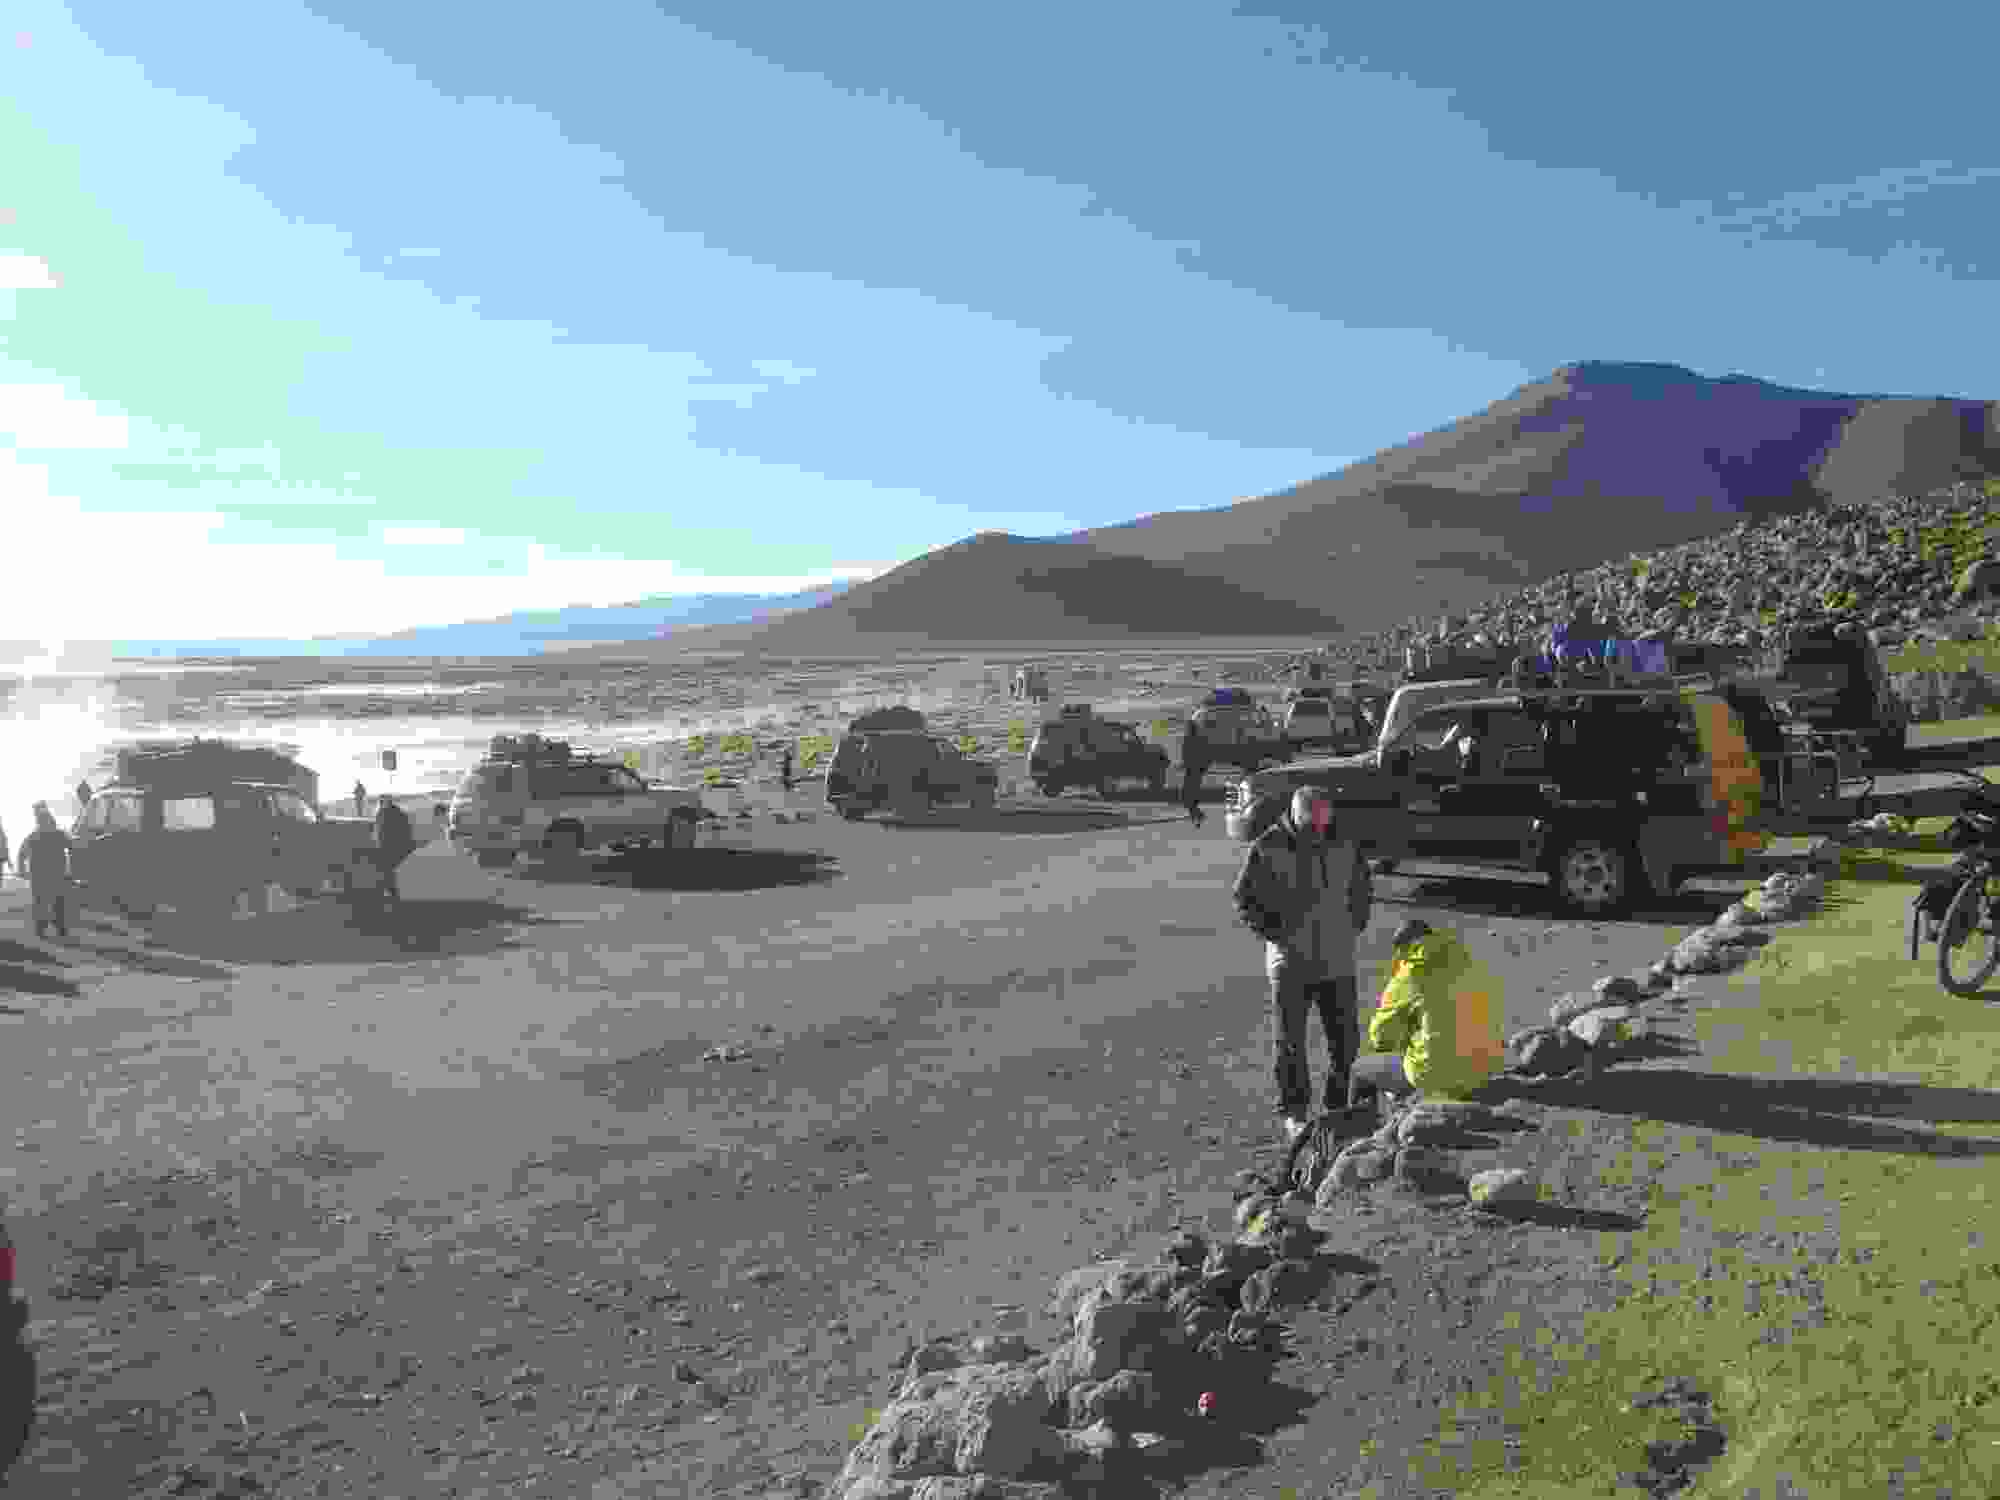
\includegraphics[width=\mywidth]{../wp-content/uploads/2015/04/wpid-wp-1427987293614.jpg} \end{center}

 20km de belle montée.
\begin{center} 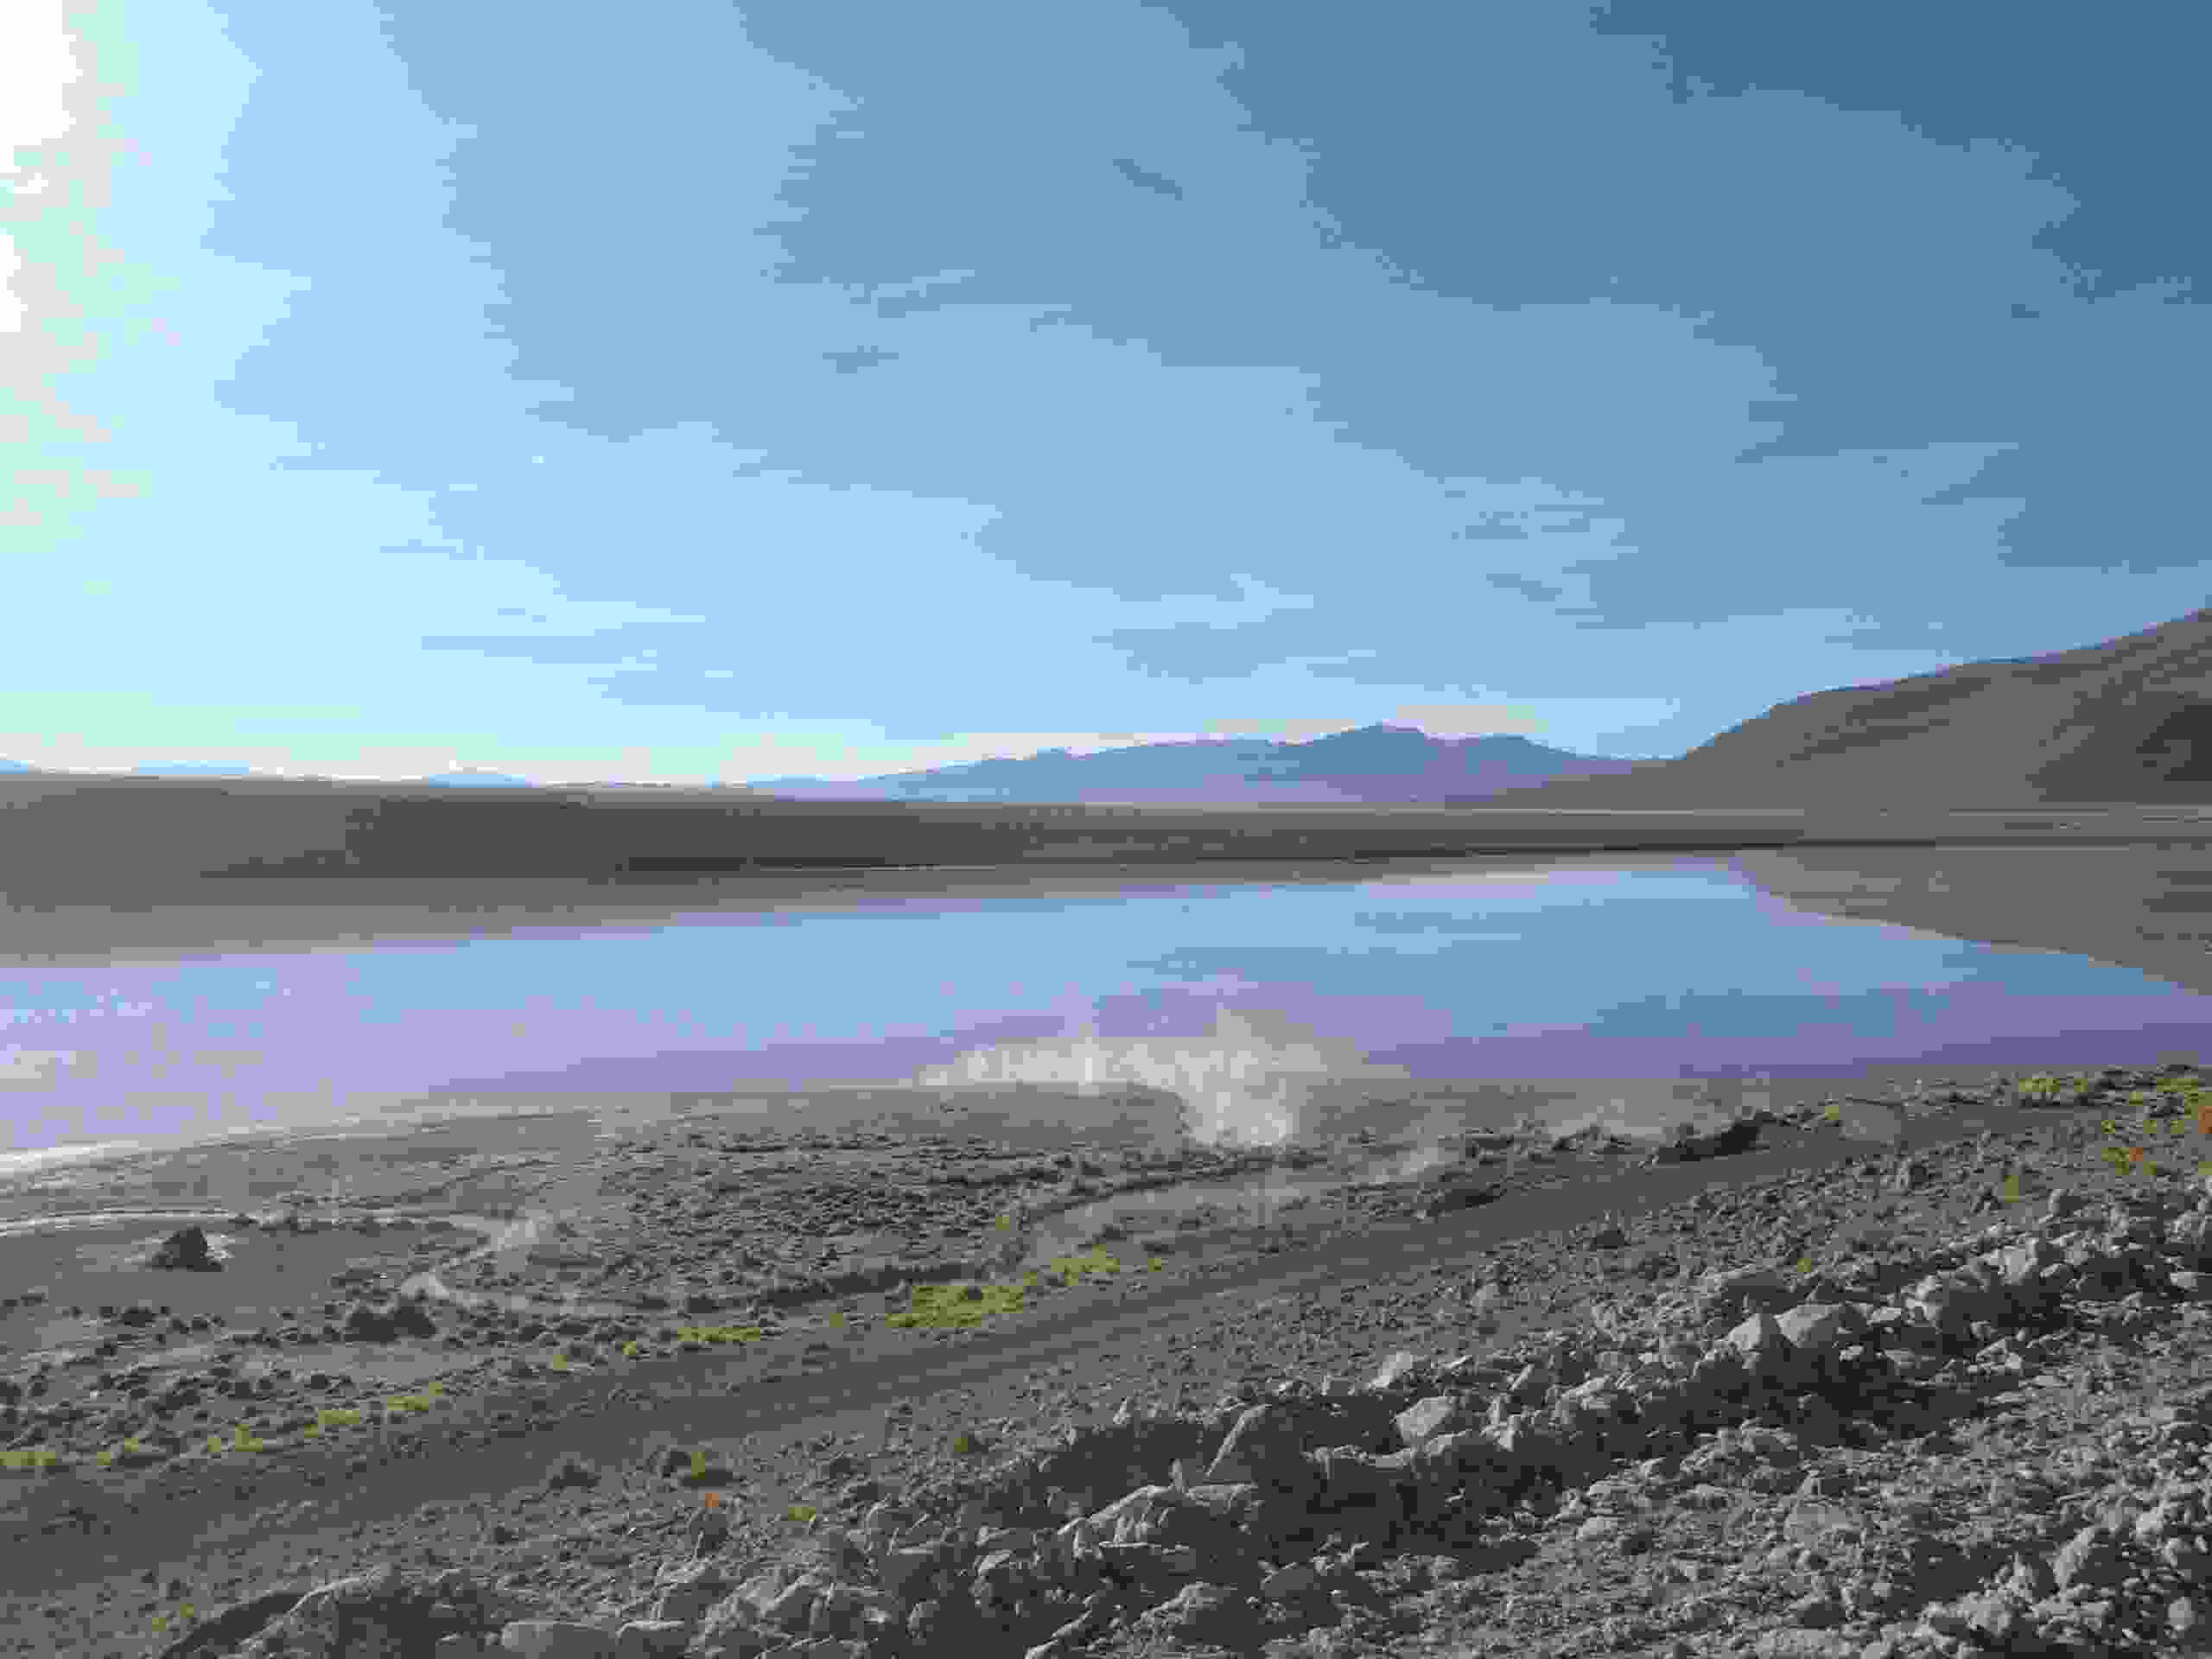
\includegraphics[width=\mywidth]{../wp-content/uploads/2015/04/wpid-wp-1427984607804.jpg} \end{center}
\begin{center} 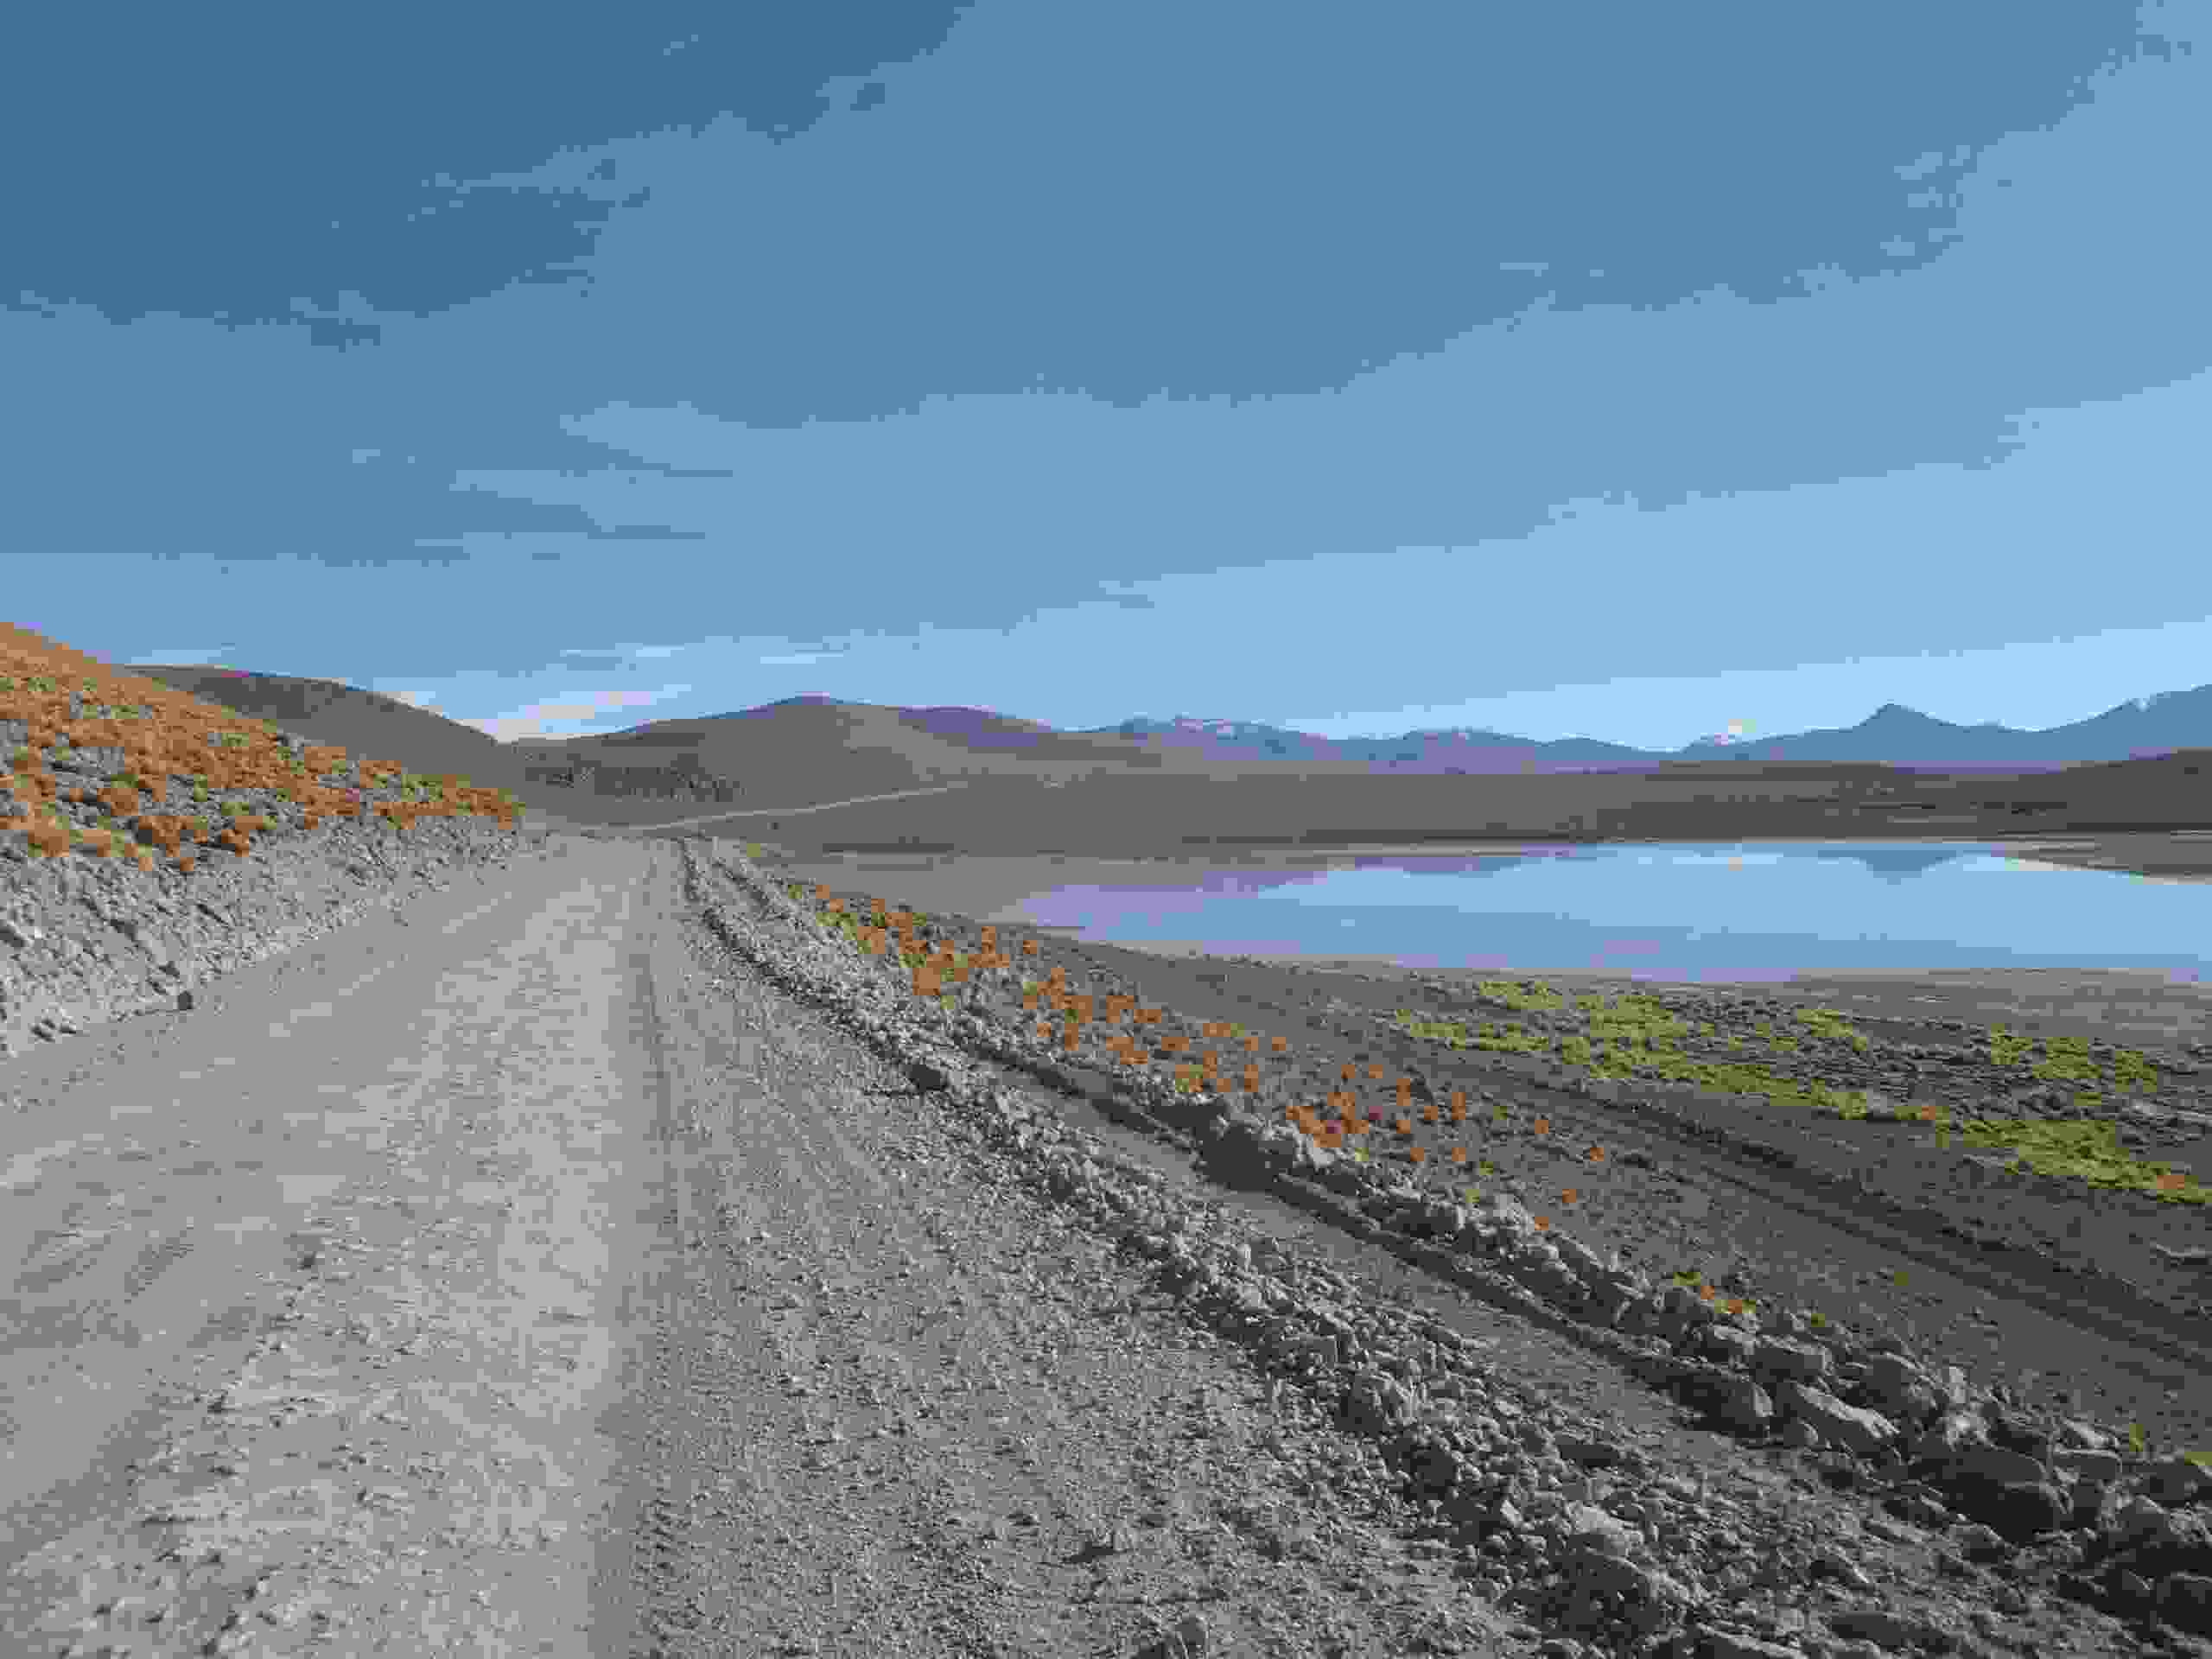
\includegraphics[width=\mywidth]{../wp-content/uploads/2015/04/wpid-wp-1427984674366.jpg} \end{center}
\begin{center} 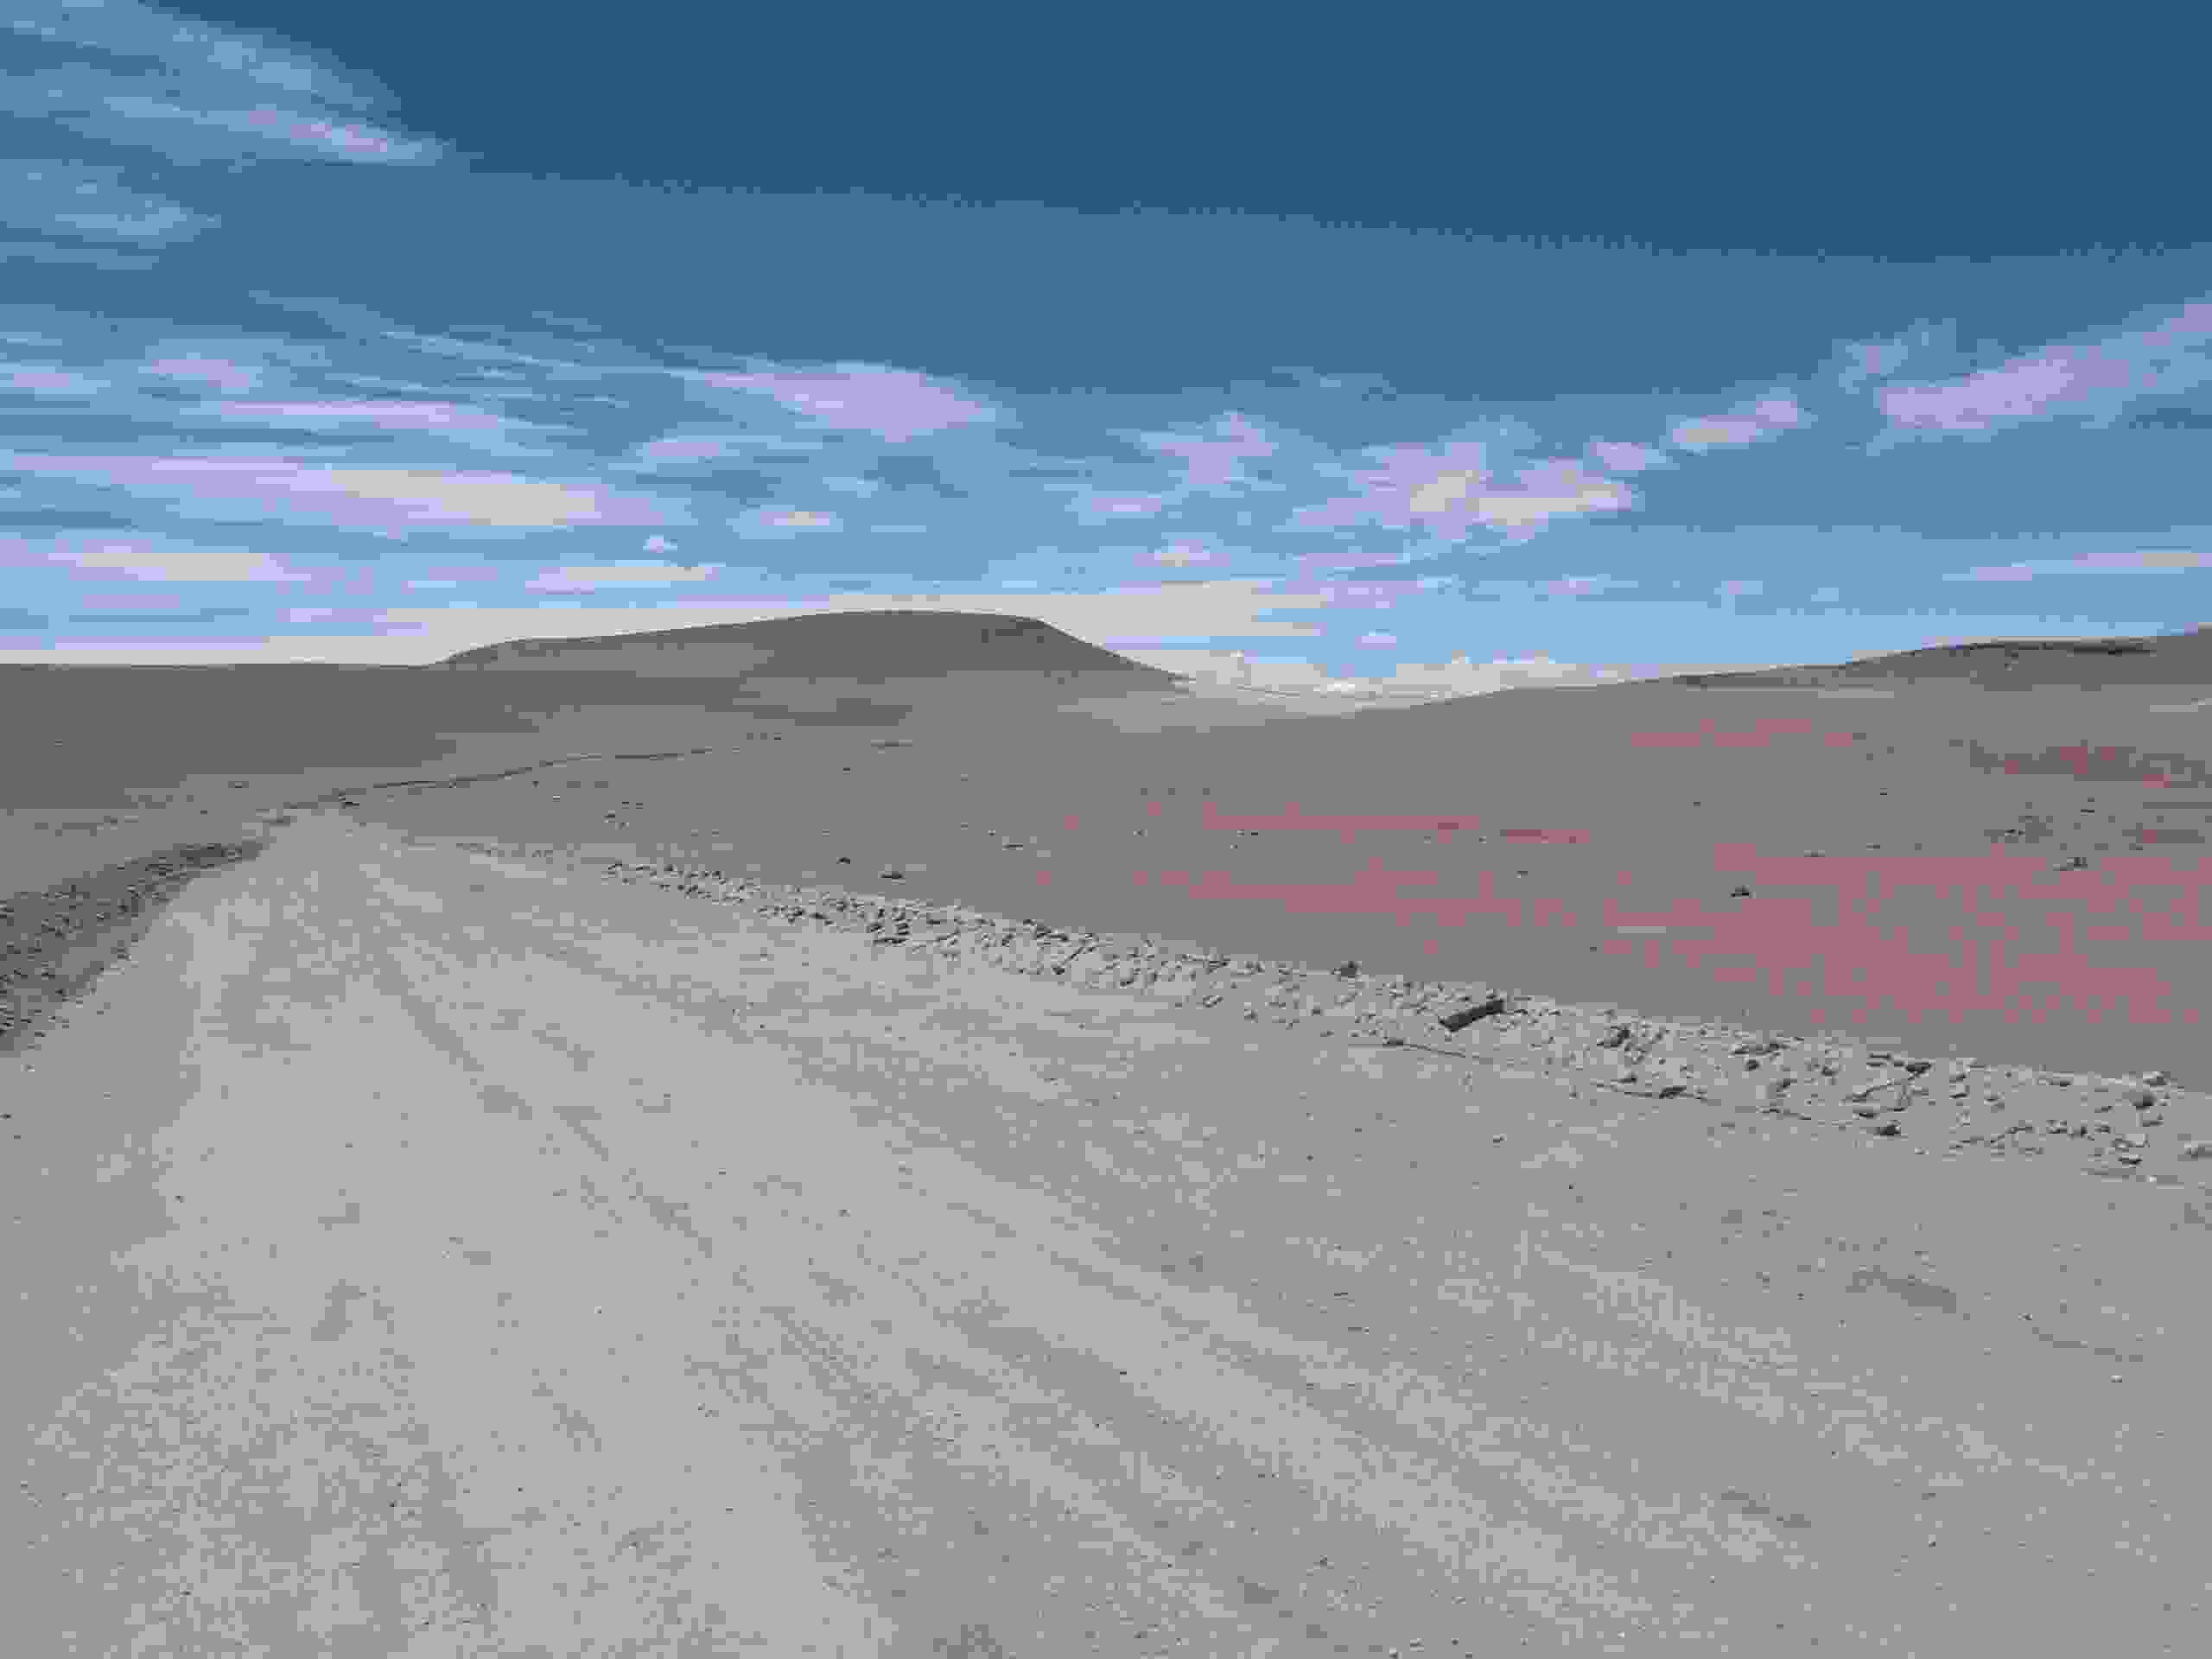
\includegraphics[width=\mywidth]{../wp-content/uploads/2015/04/wpid-wp-1427984642376.jpg} \end{center}

\pagebreak
  Pour arriver au geyser de Sol de Manana à presque 5000m.
\begin{center} 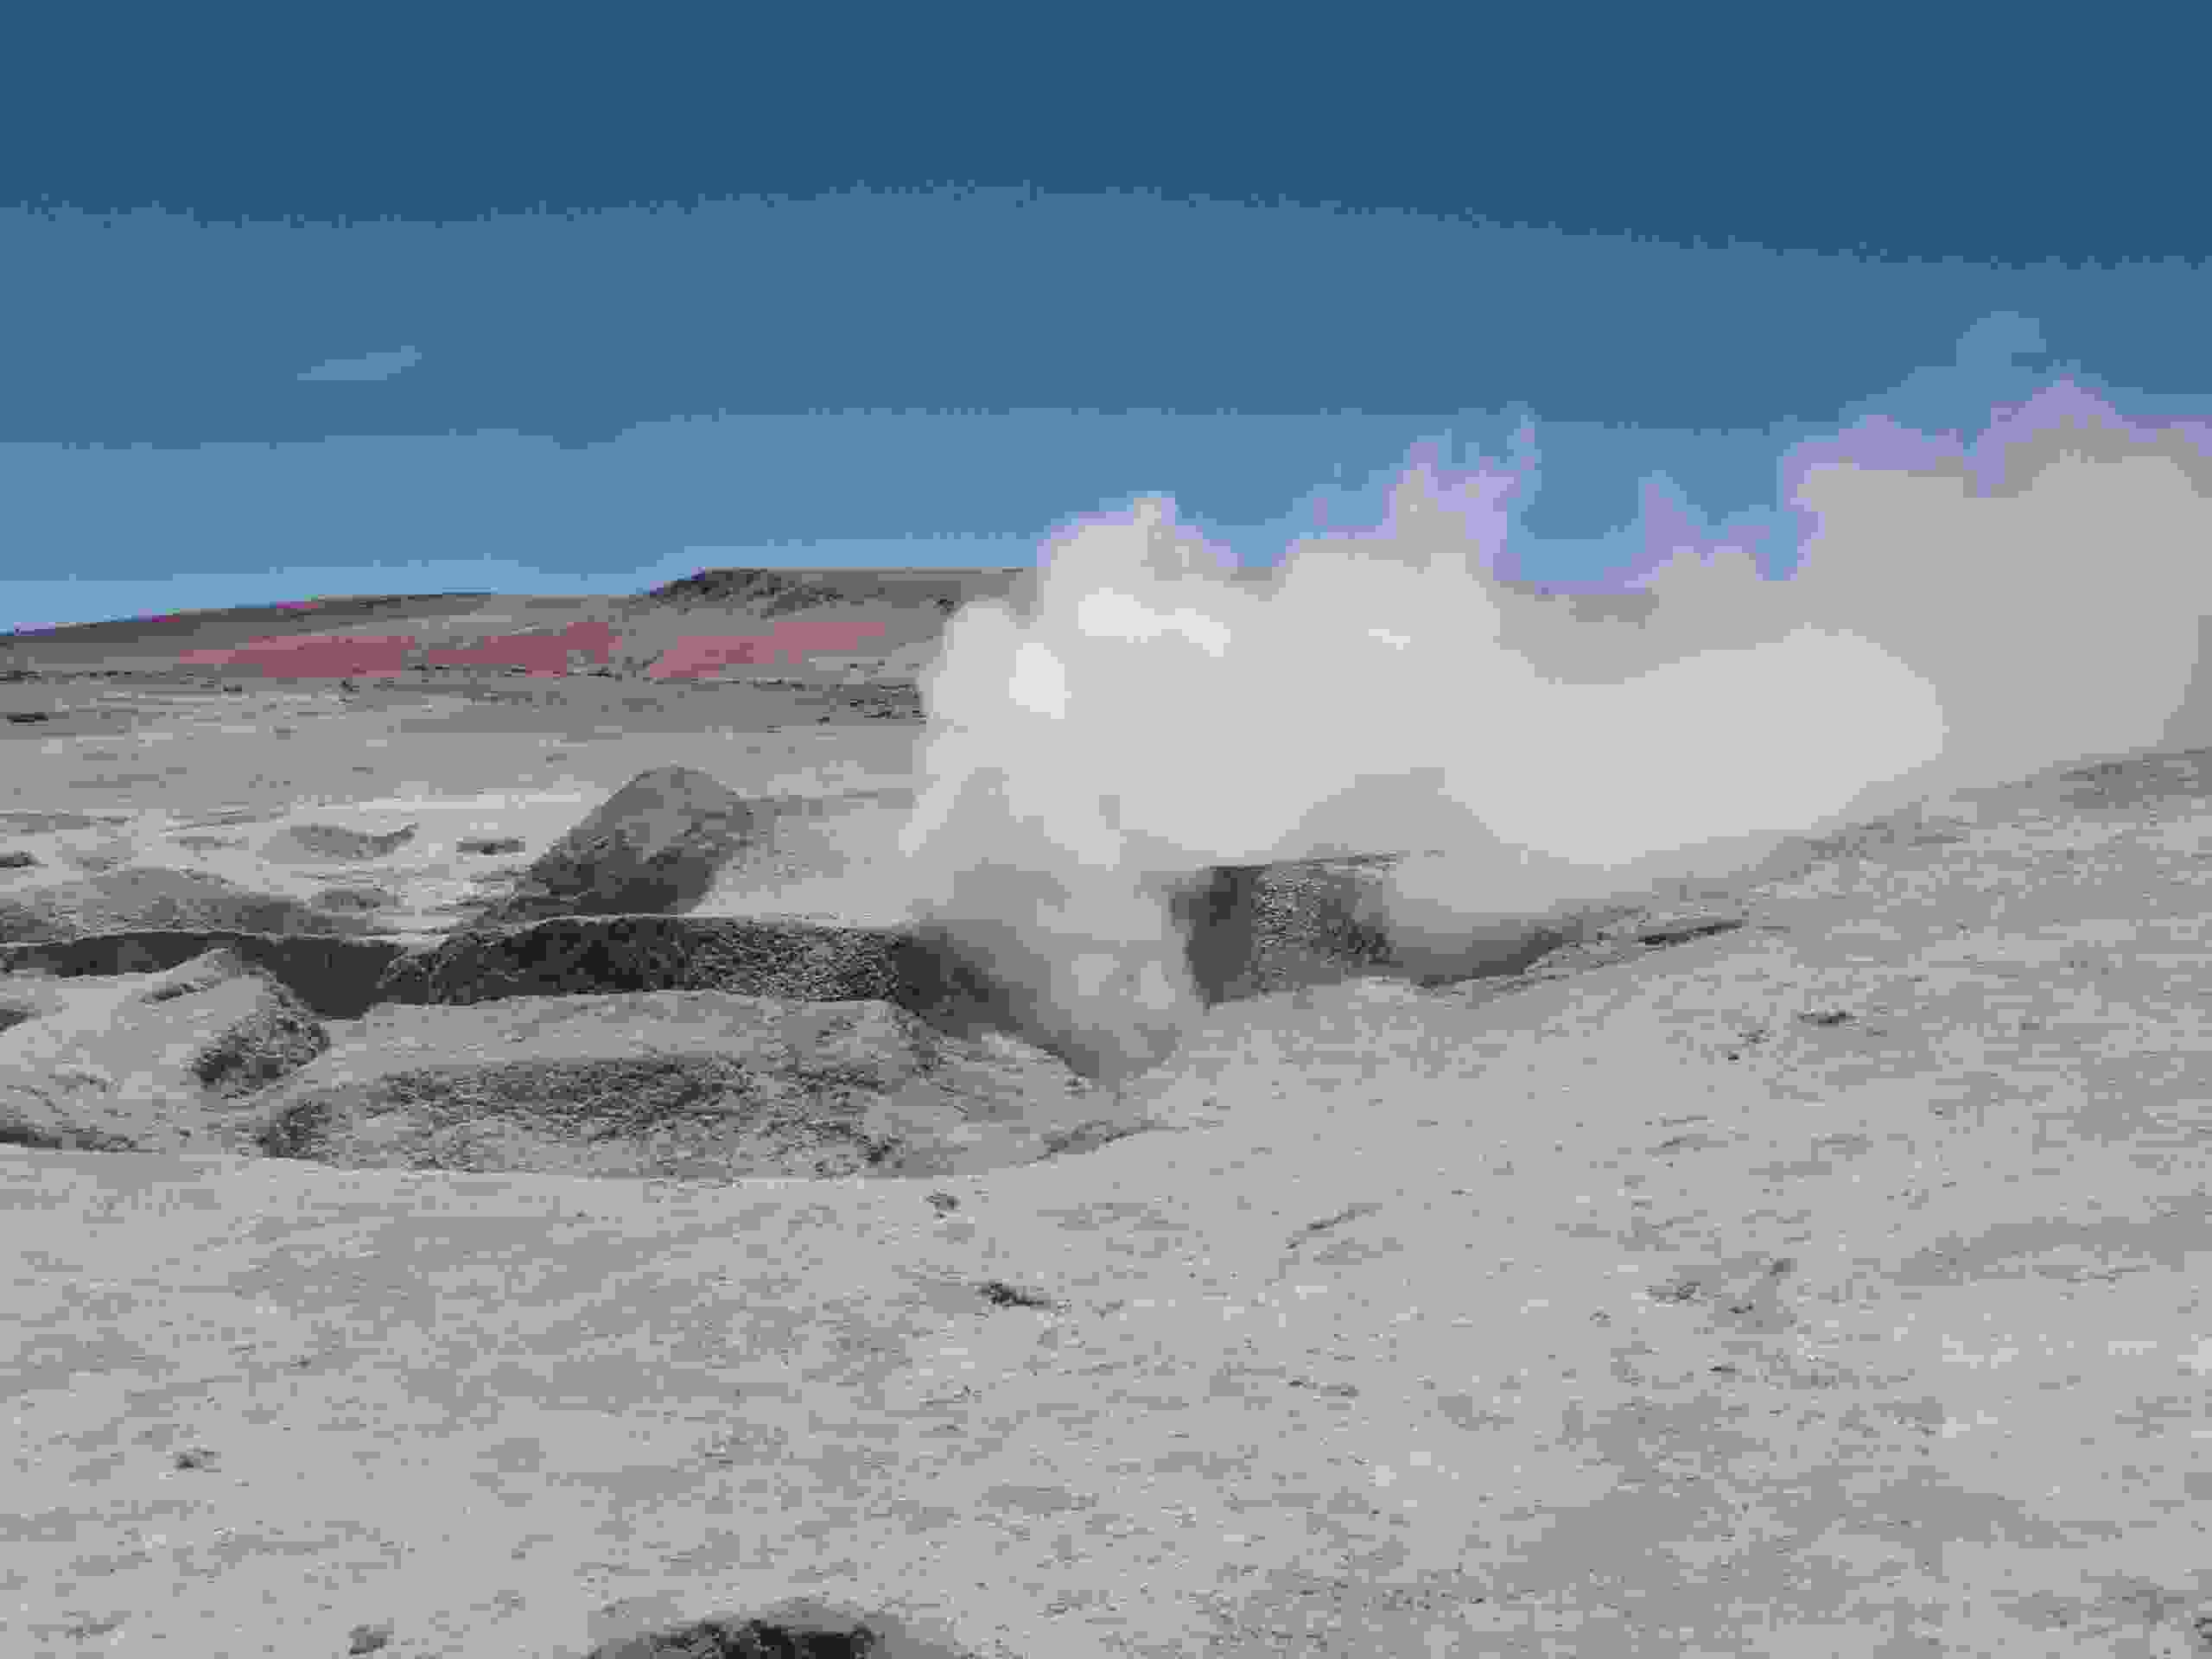
\includegraphics[width=\mywidth]{../wp-content/uploads/2015/04/wpid-wp-1427984711818.jpg} \end{center}
\begin{center} 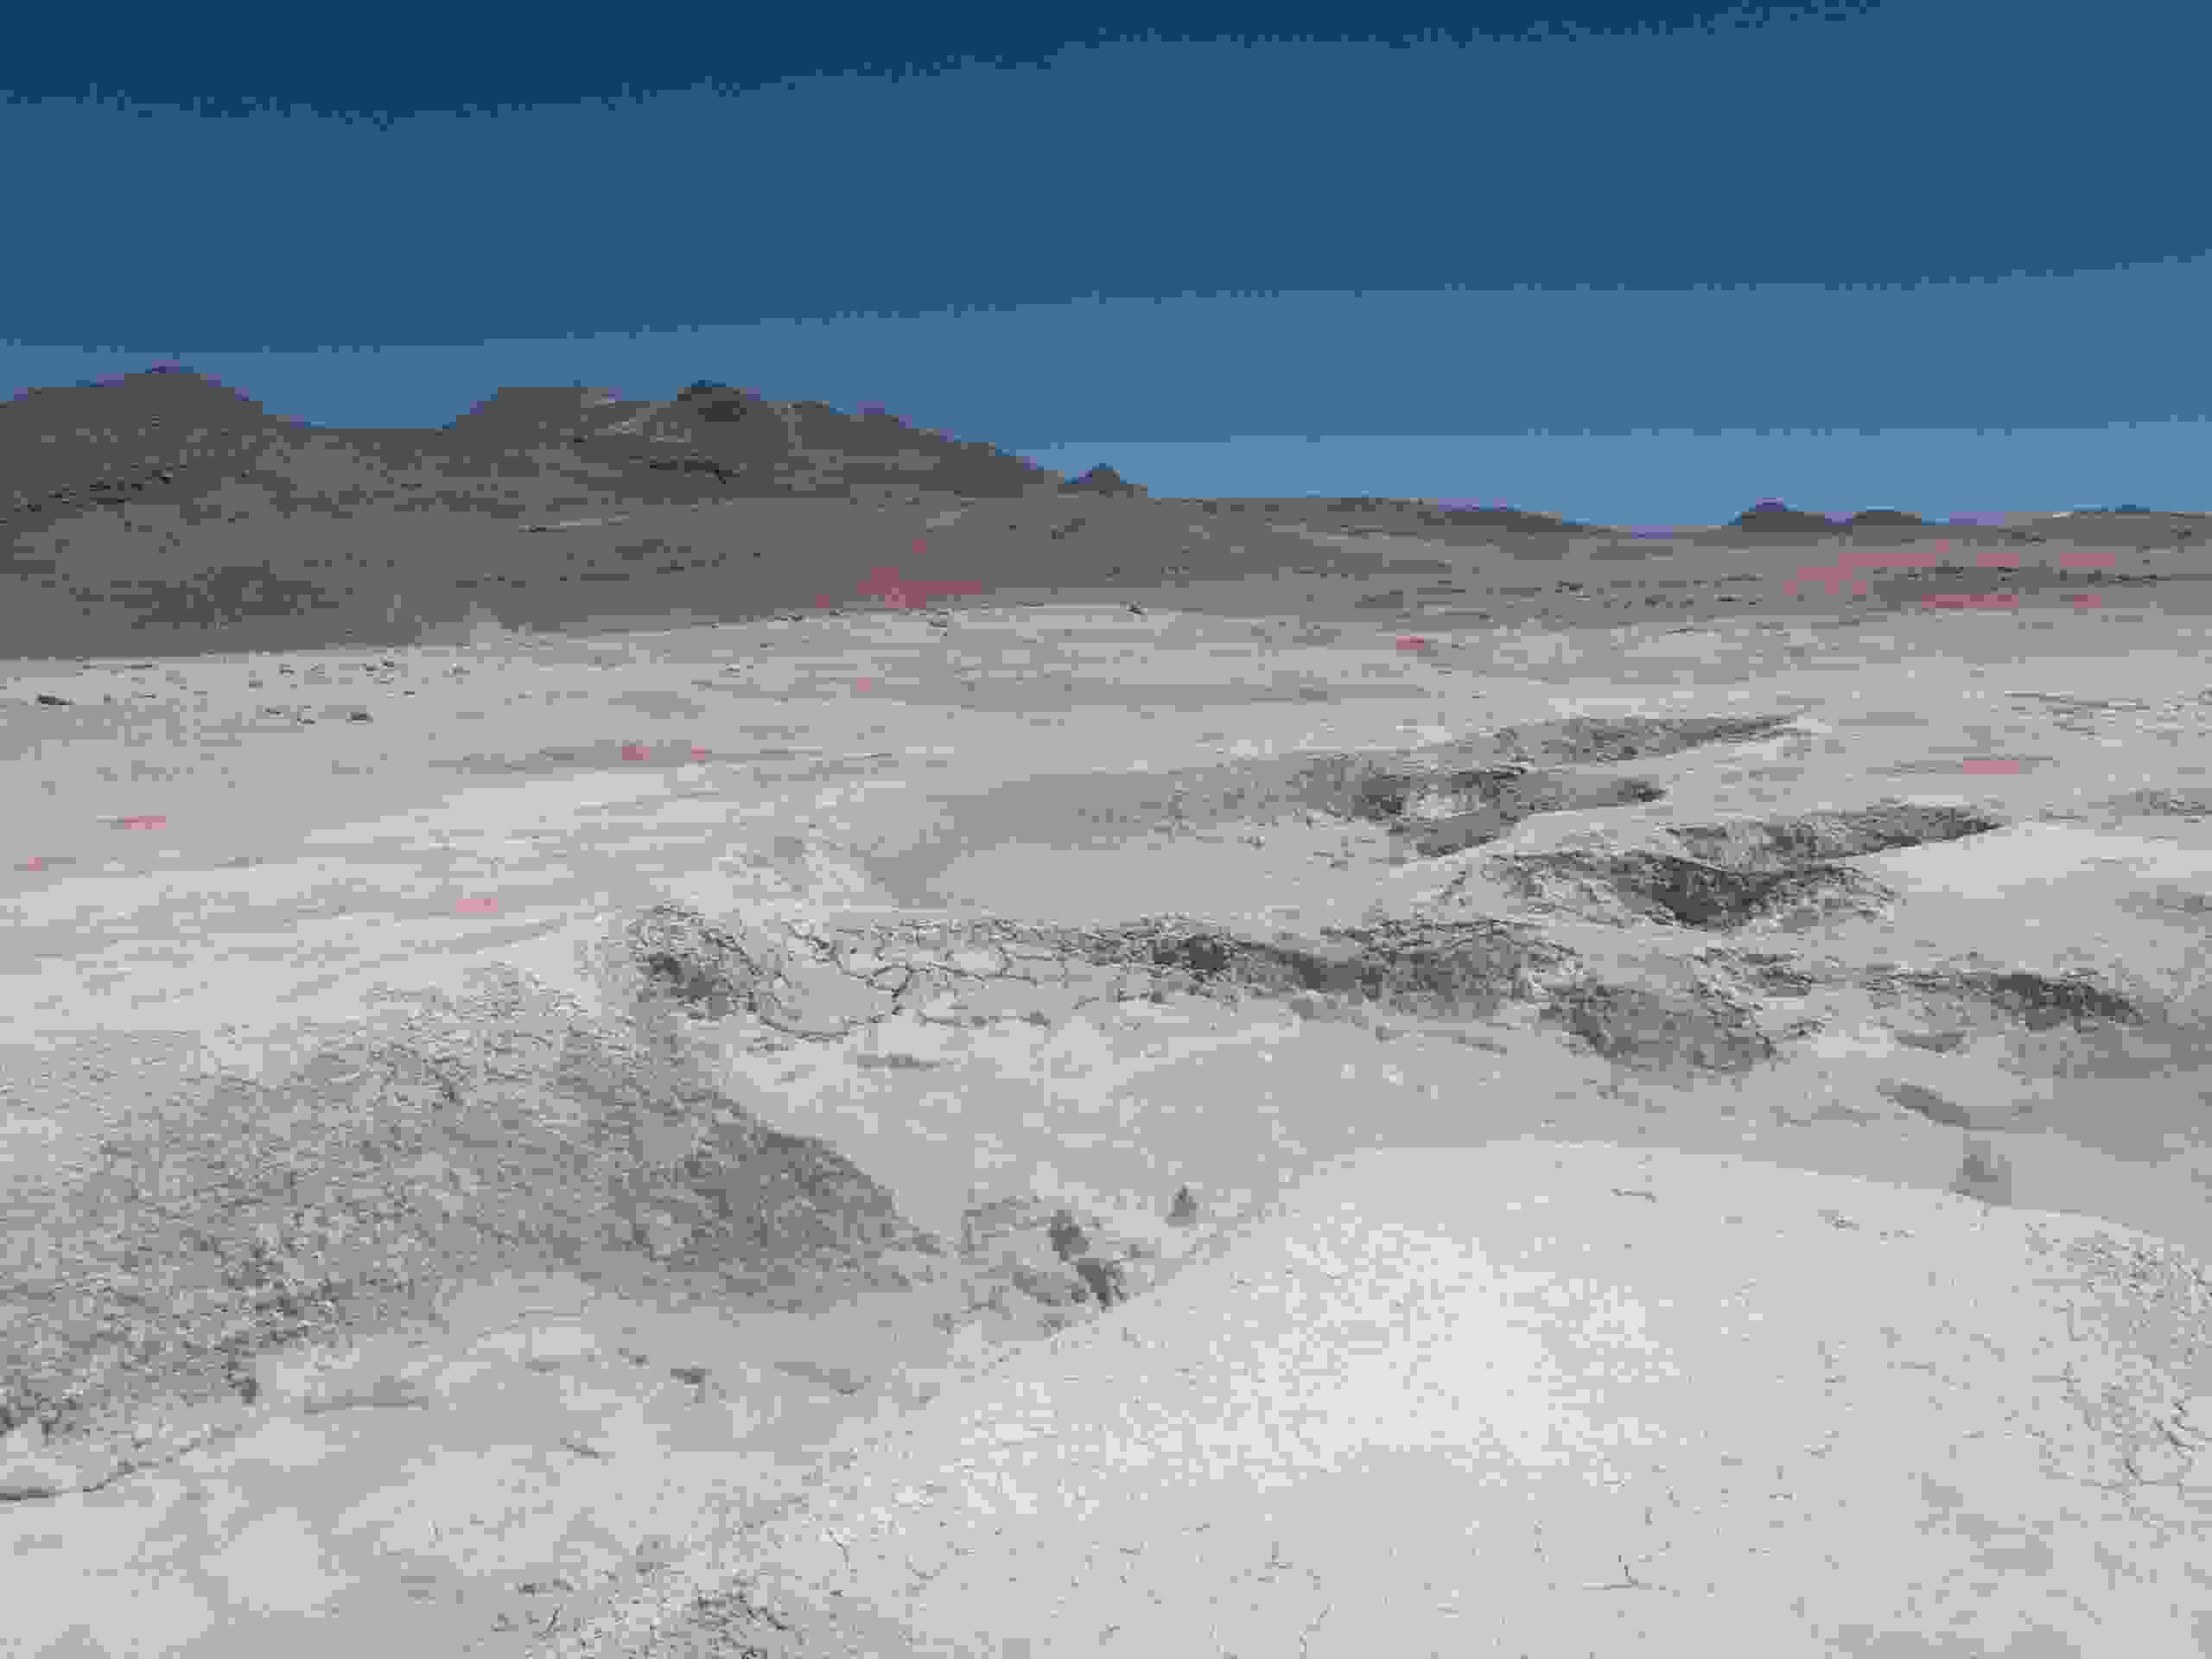
\includegraphics[width=\mywidth]{../wp-content/uploads/2015/04/wpid-wp-1427984728203.jpg} \end{center}
\begin{center} 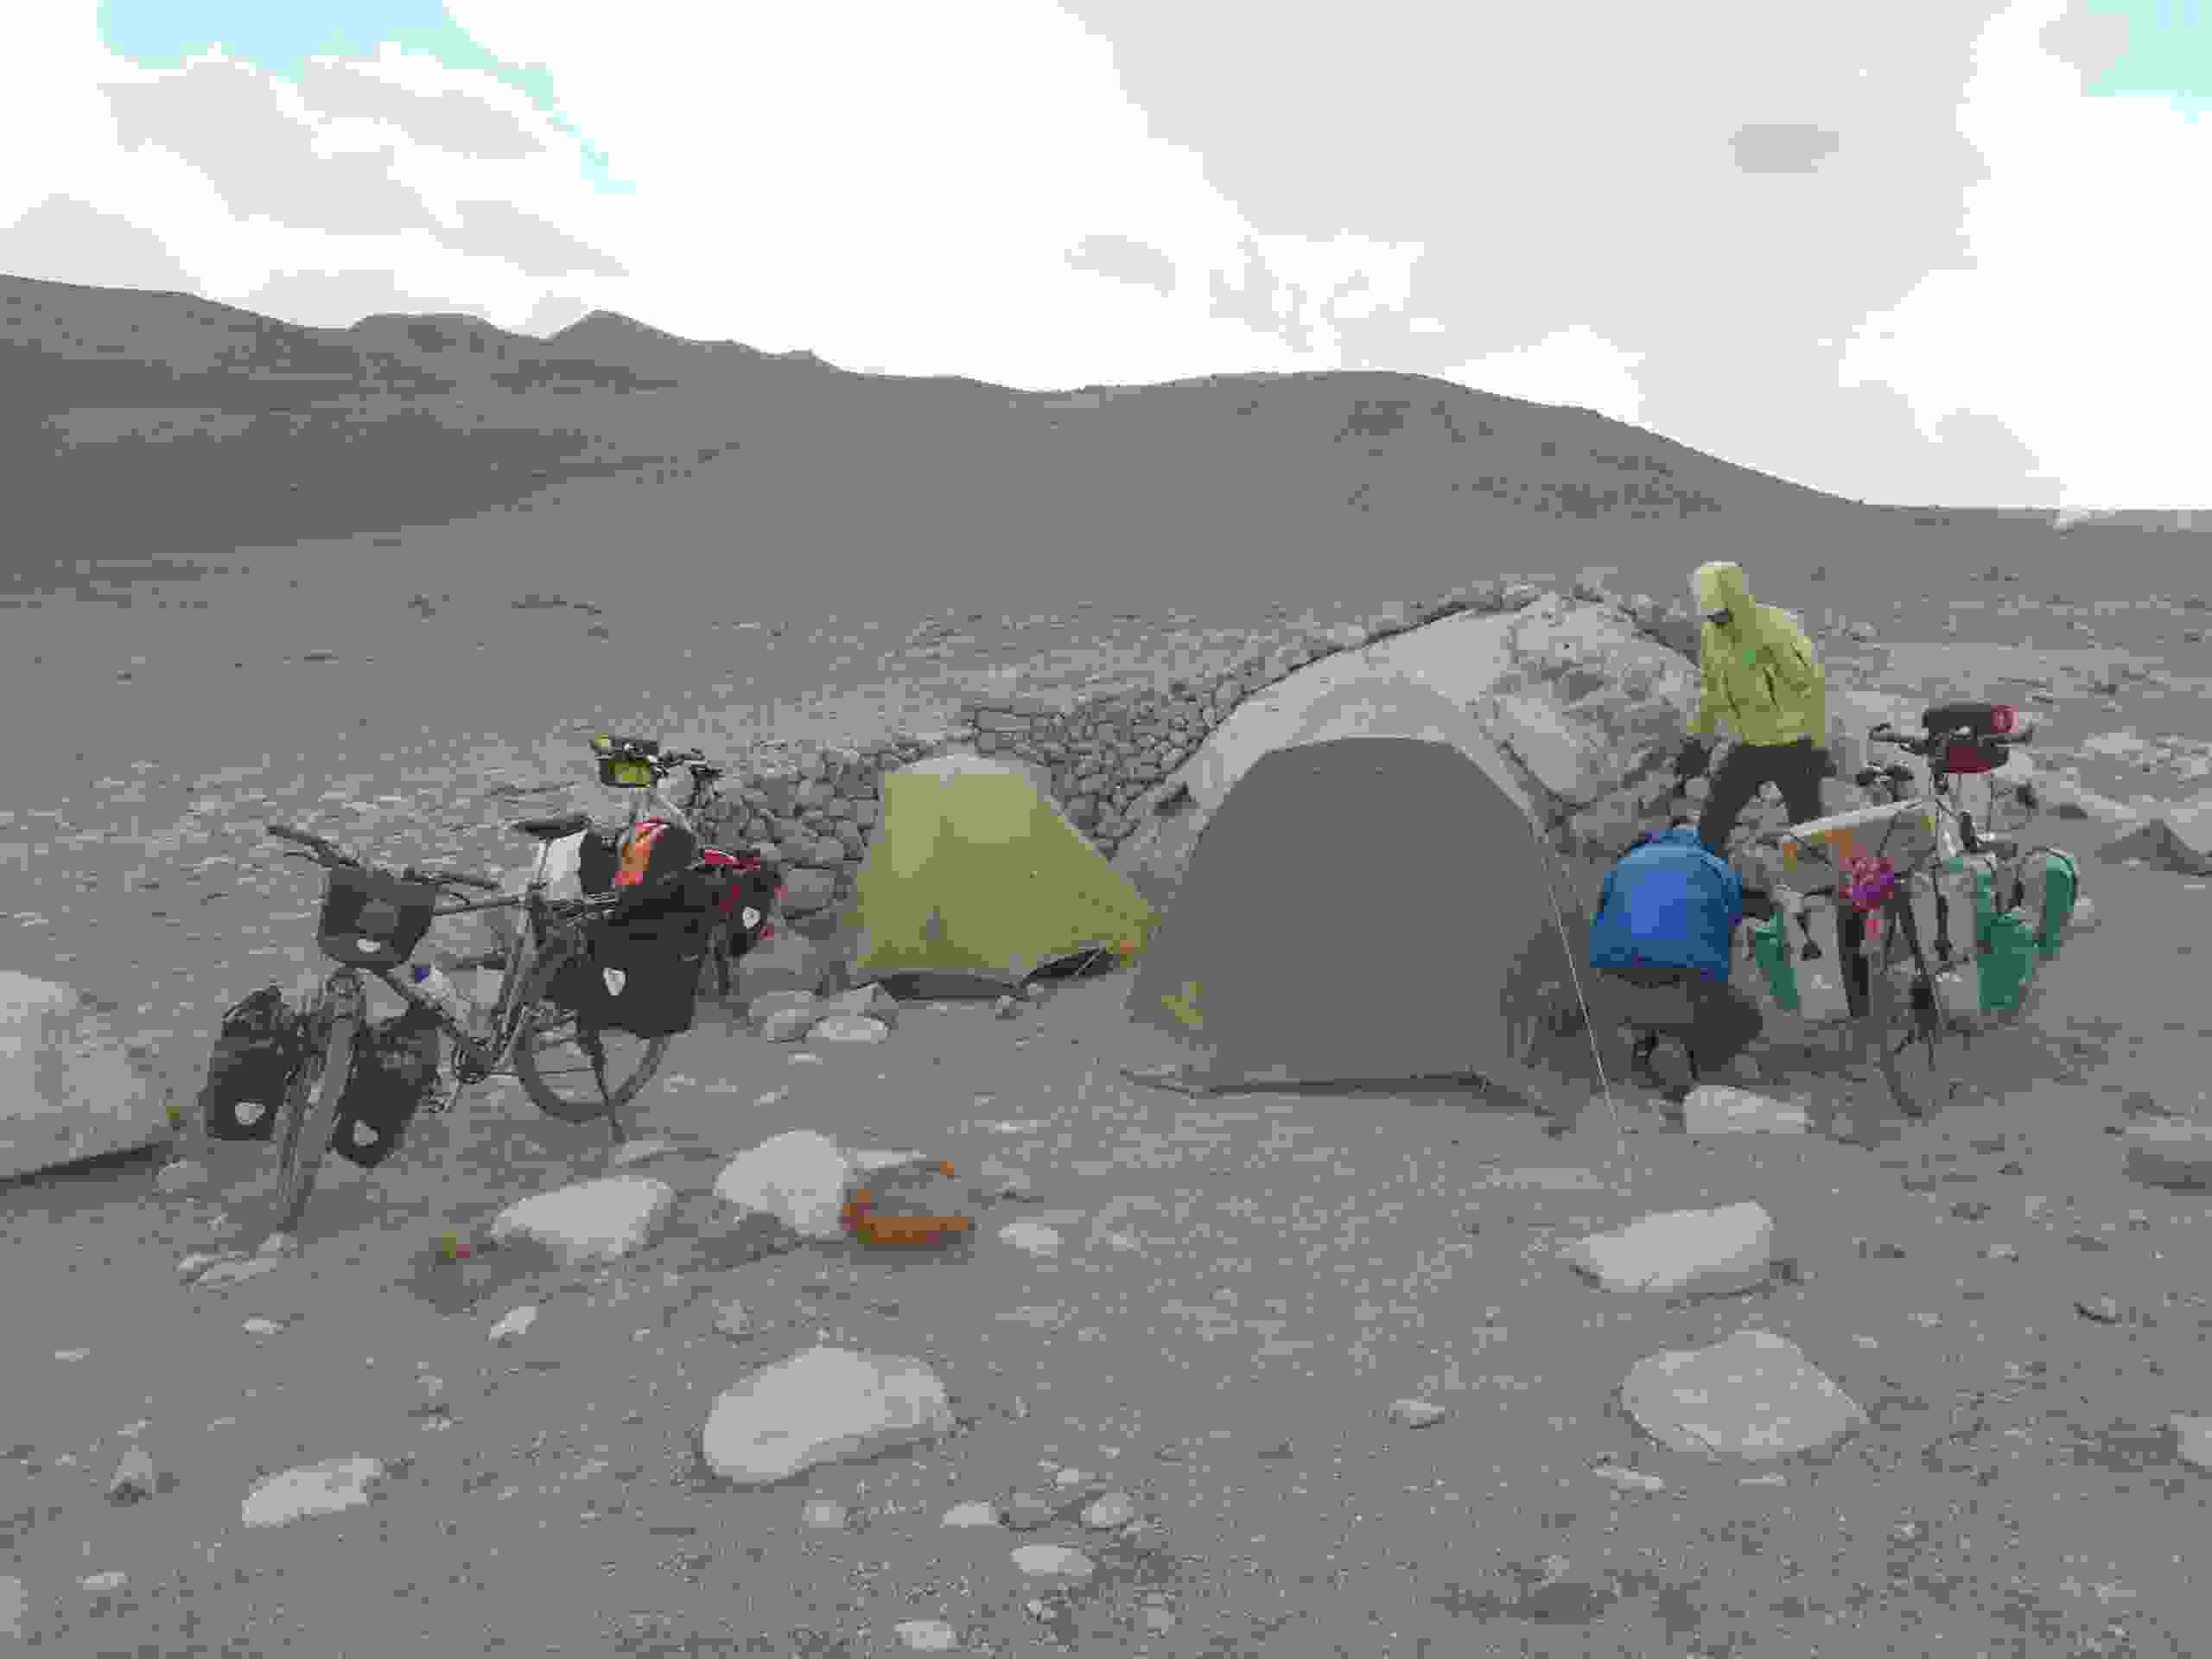
\includegraphics[width=\mywidth]{../wp-content/uploads/2015/04/wpid-wp-1427984752108.jpg} \end{center}

 \subsection*{4\ieme\ jour} 

 Froid et vent de face, la galère commence.
\begin{center} 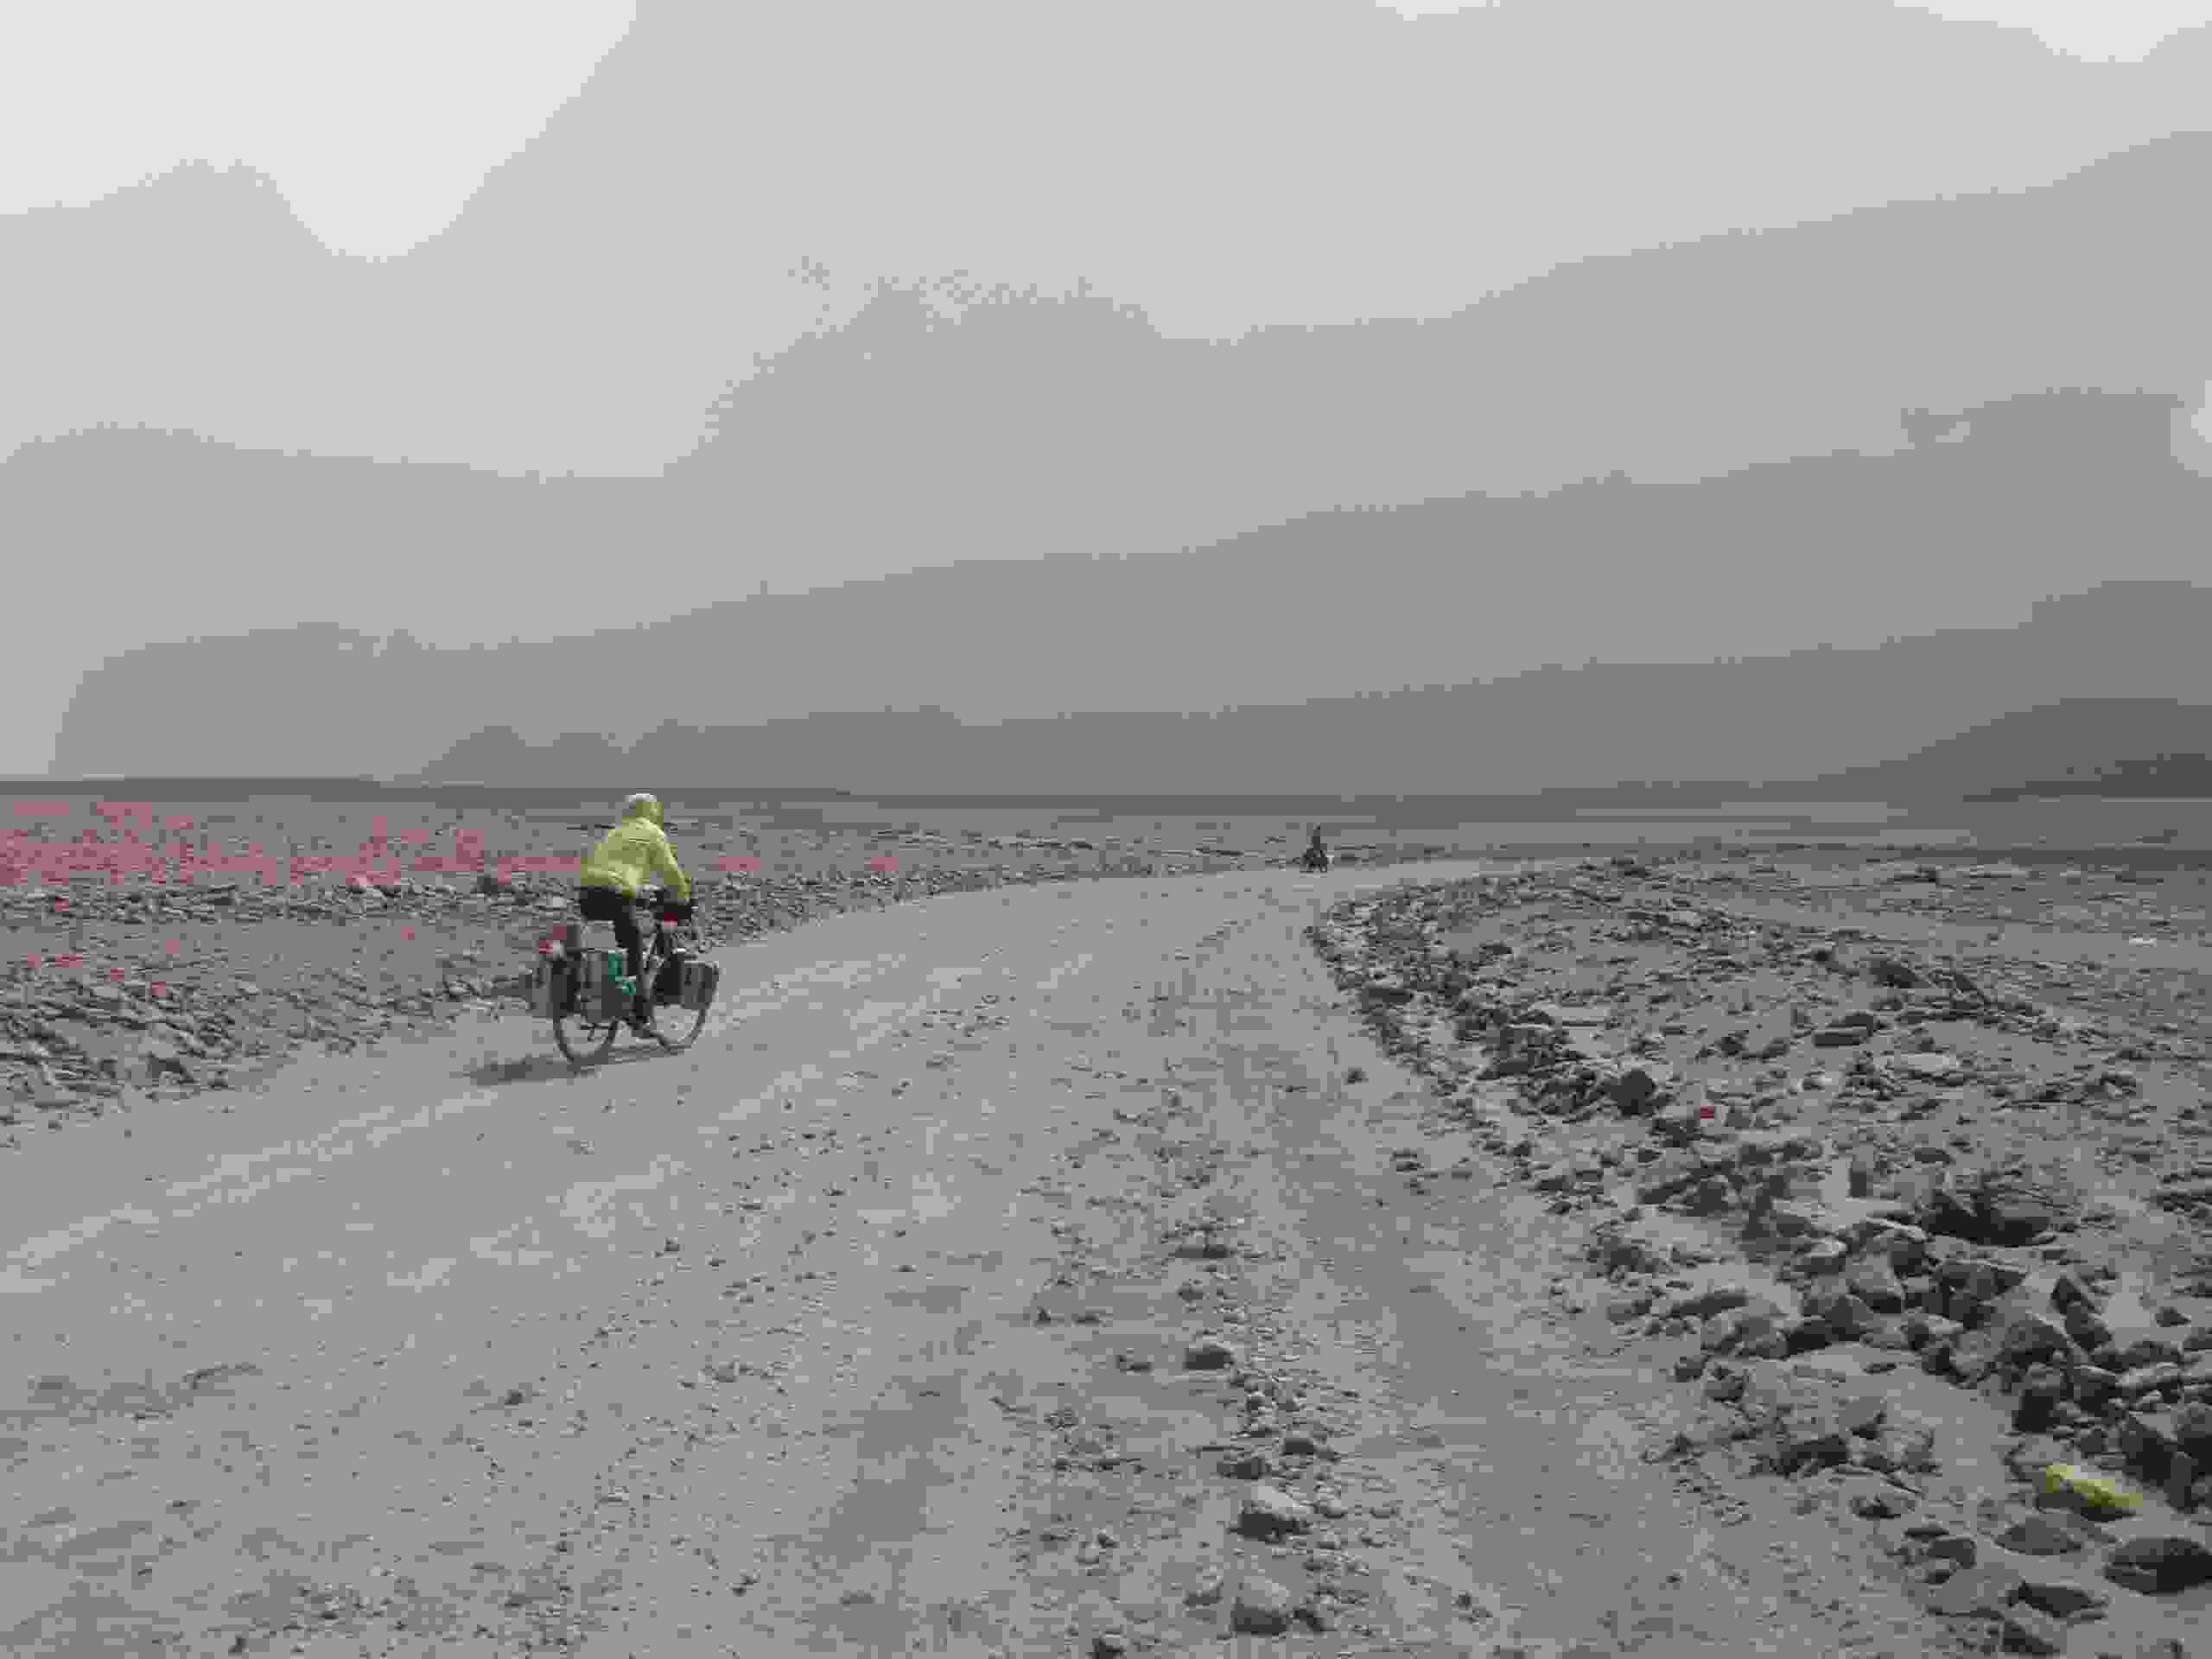
\includegraphics[width=\mywidth]{../wp-content/uploads/2015/04/wpid-wp-1427984855465.jpg} \end{center}

\pagebreak
 Heureusement les premières vues sur la Laguna Colorado compensent un peu.
\begin{center} 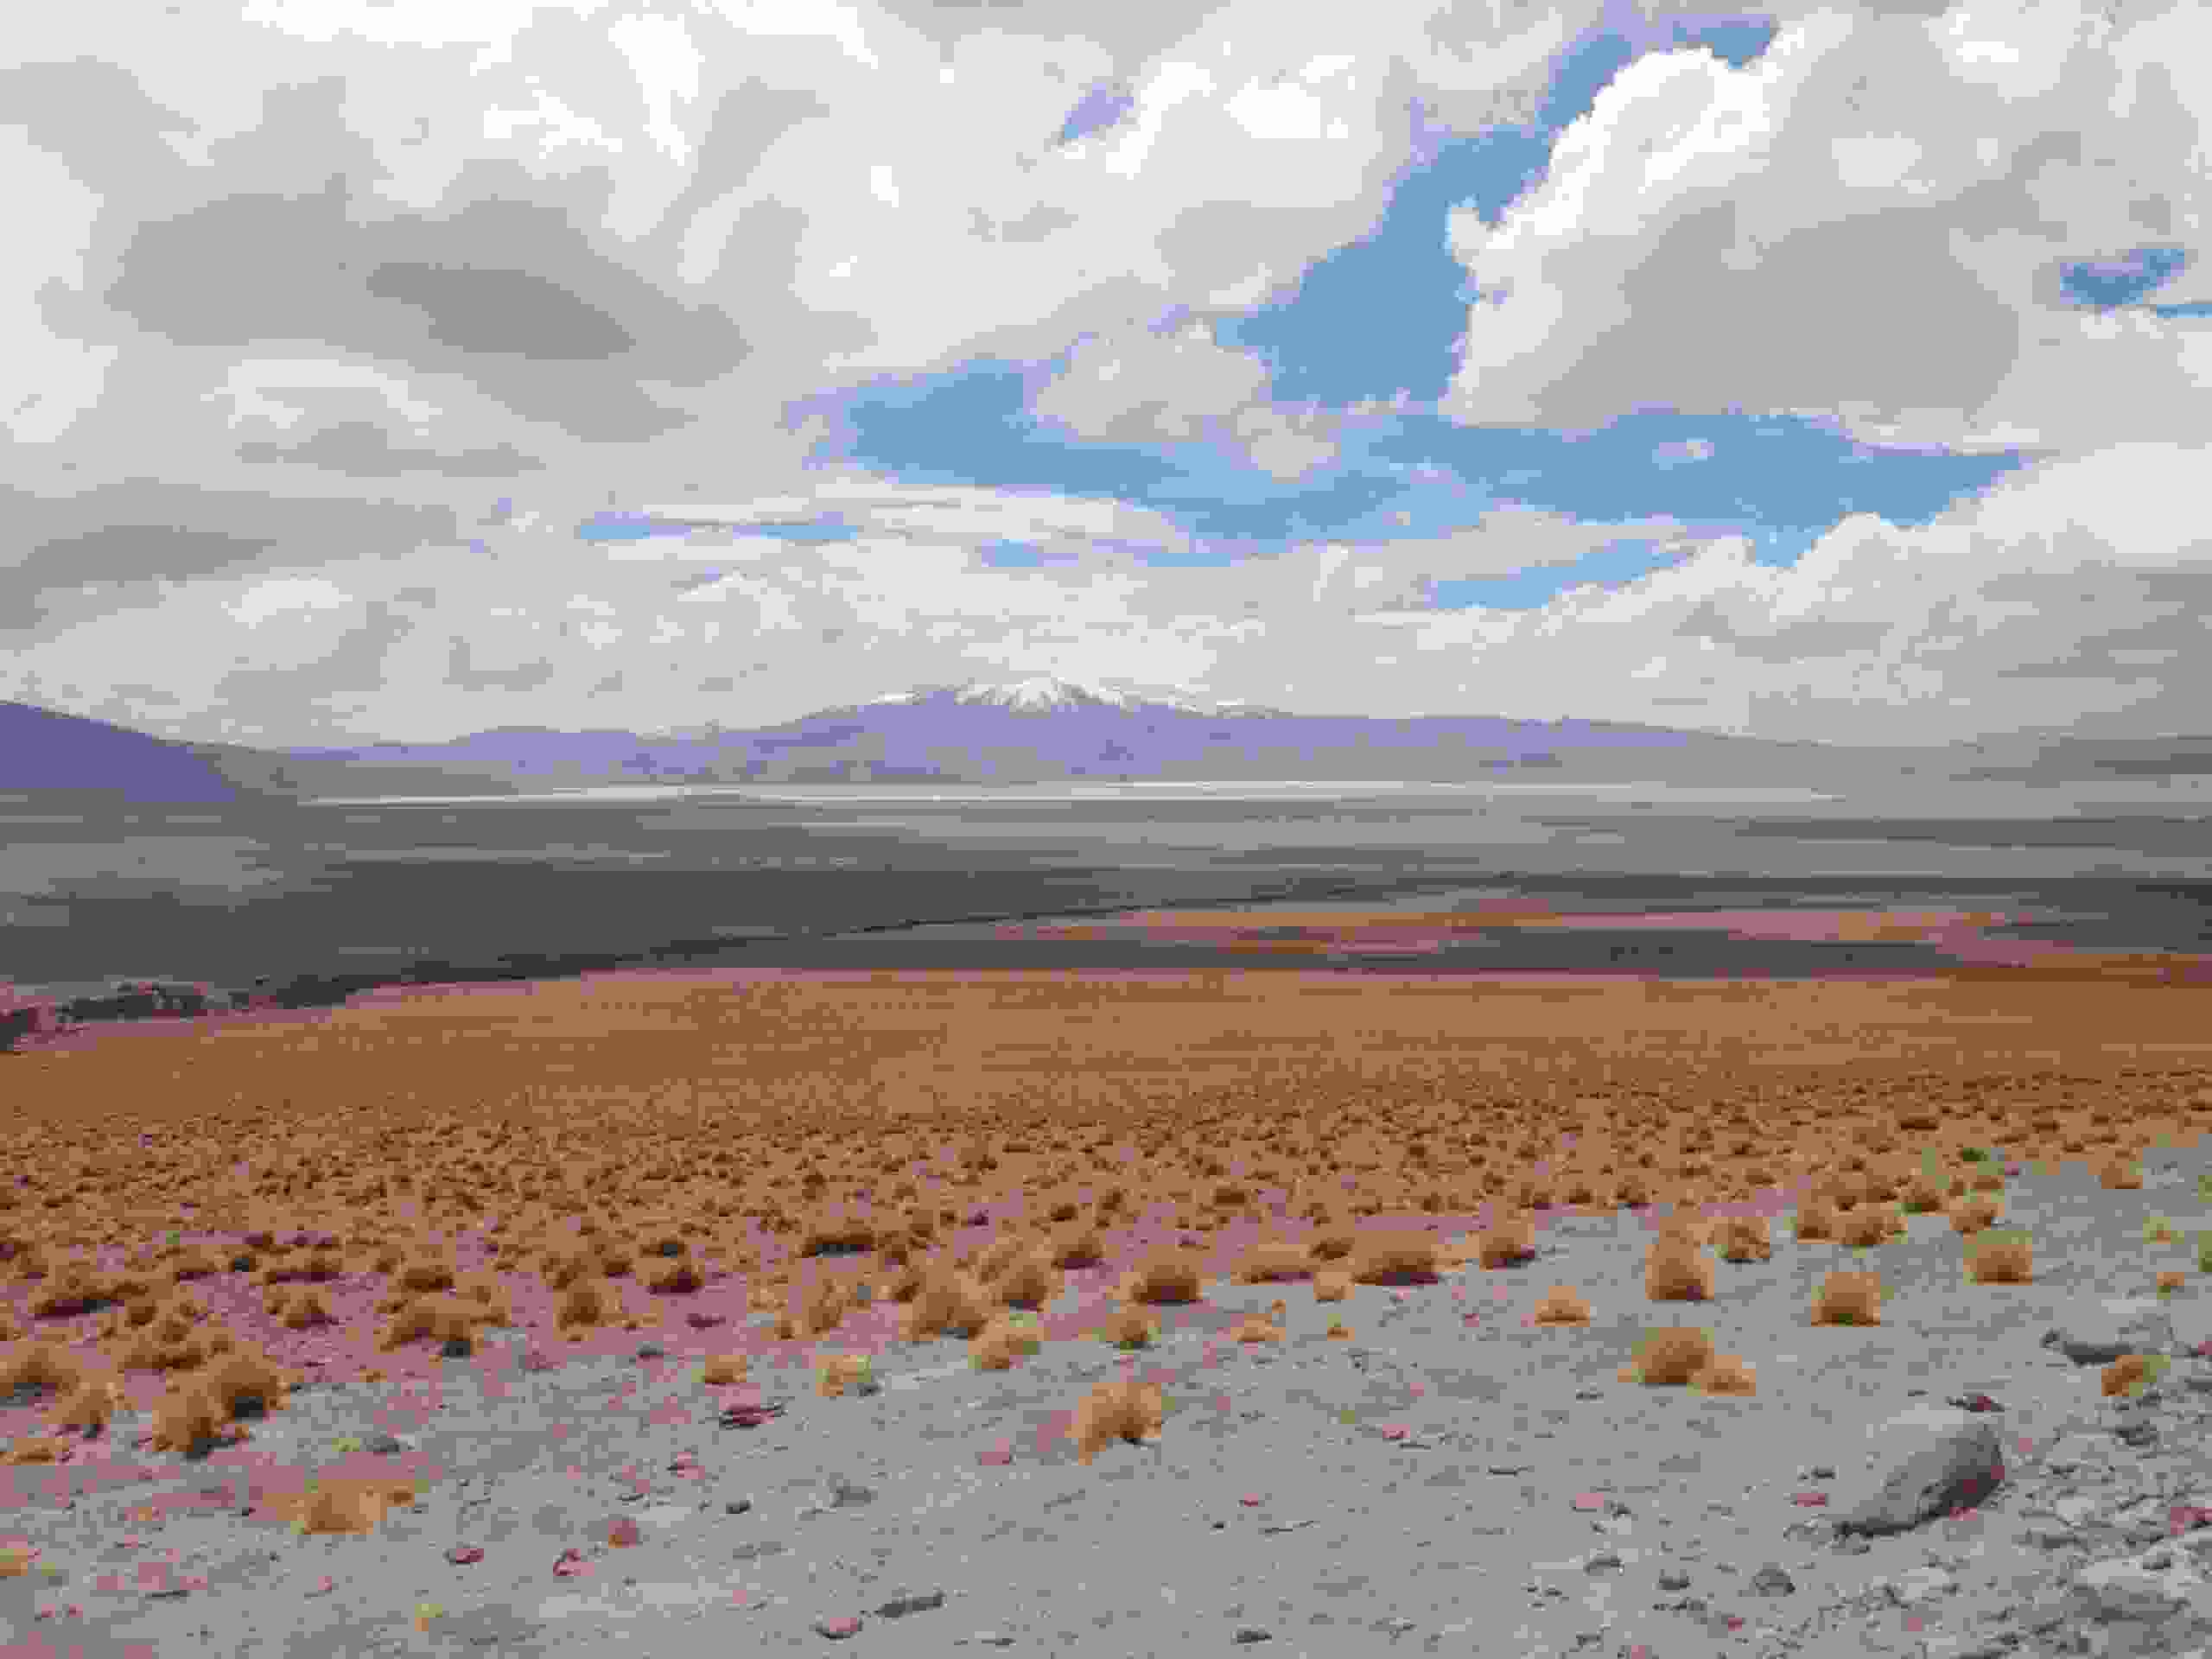
\includegraphics[width=\mywidth]{../wp-content/uploads/2015/04/wpid-wp-1427984806510.jpg} \end{center}
\begin{center} 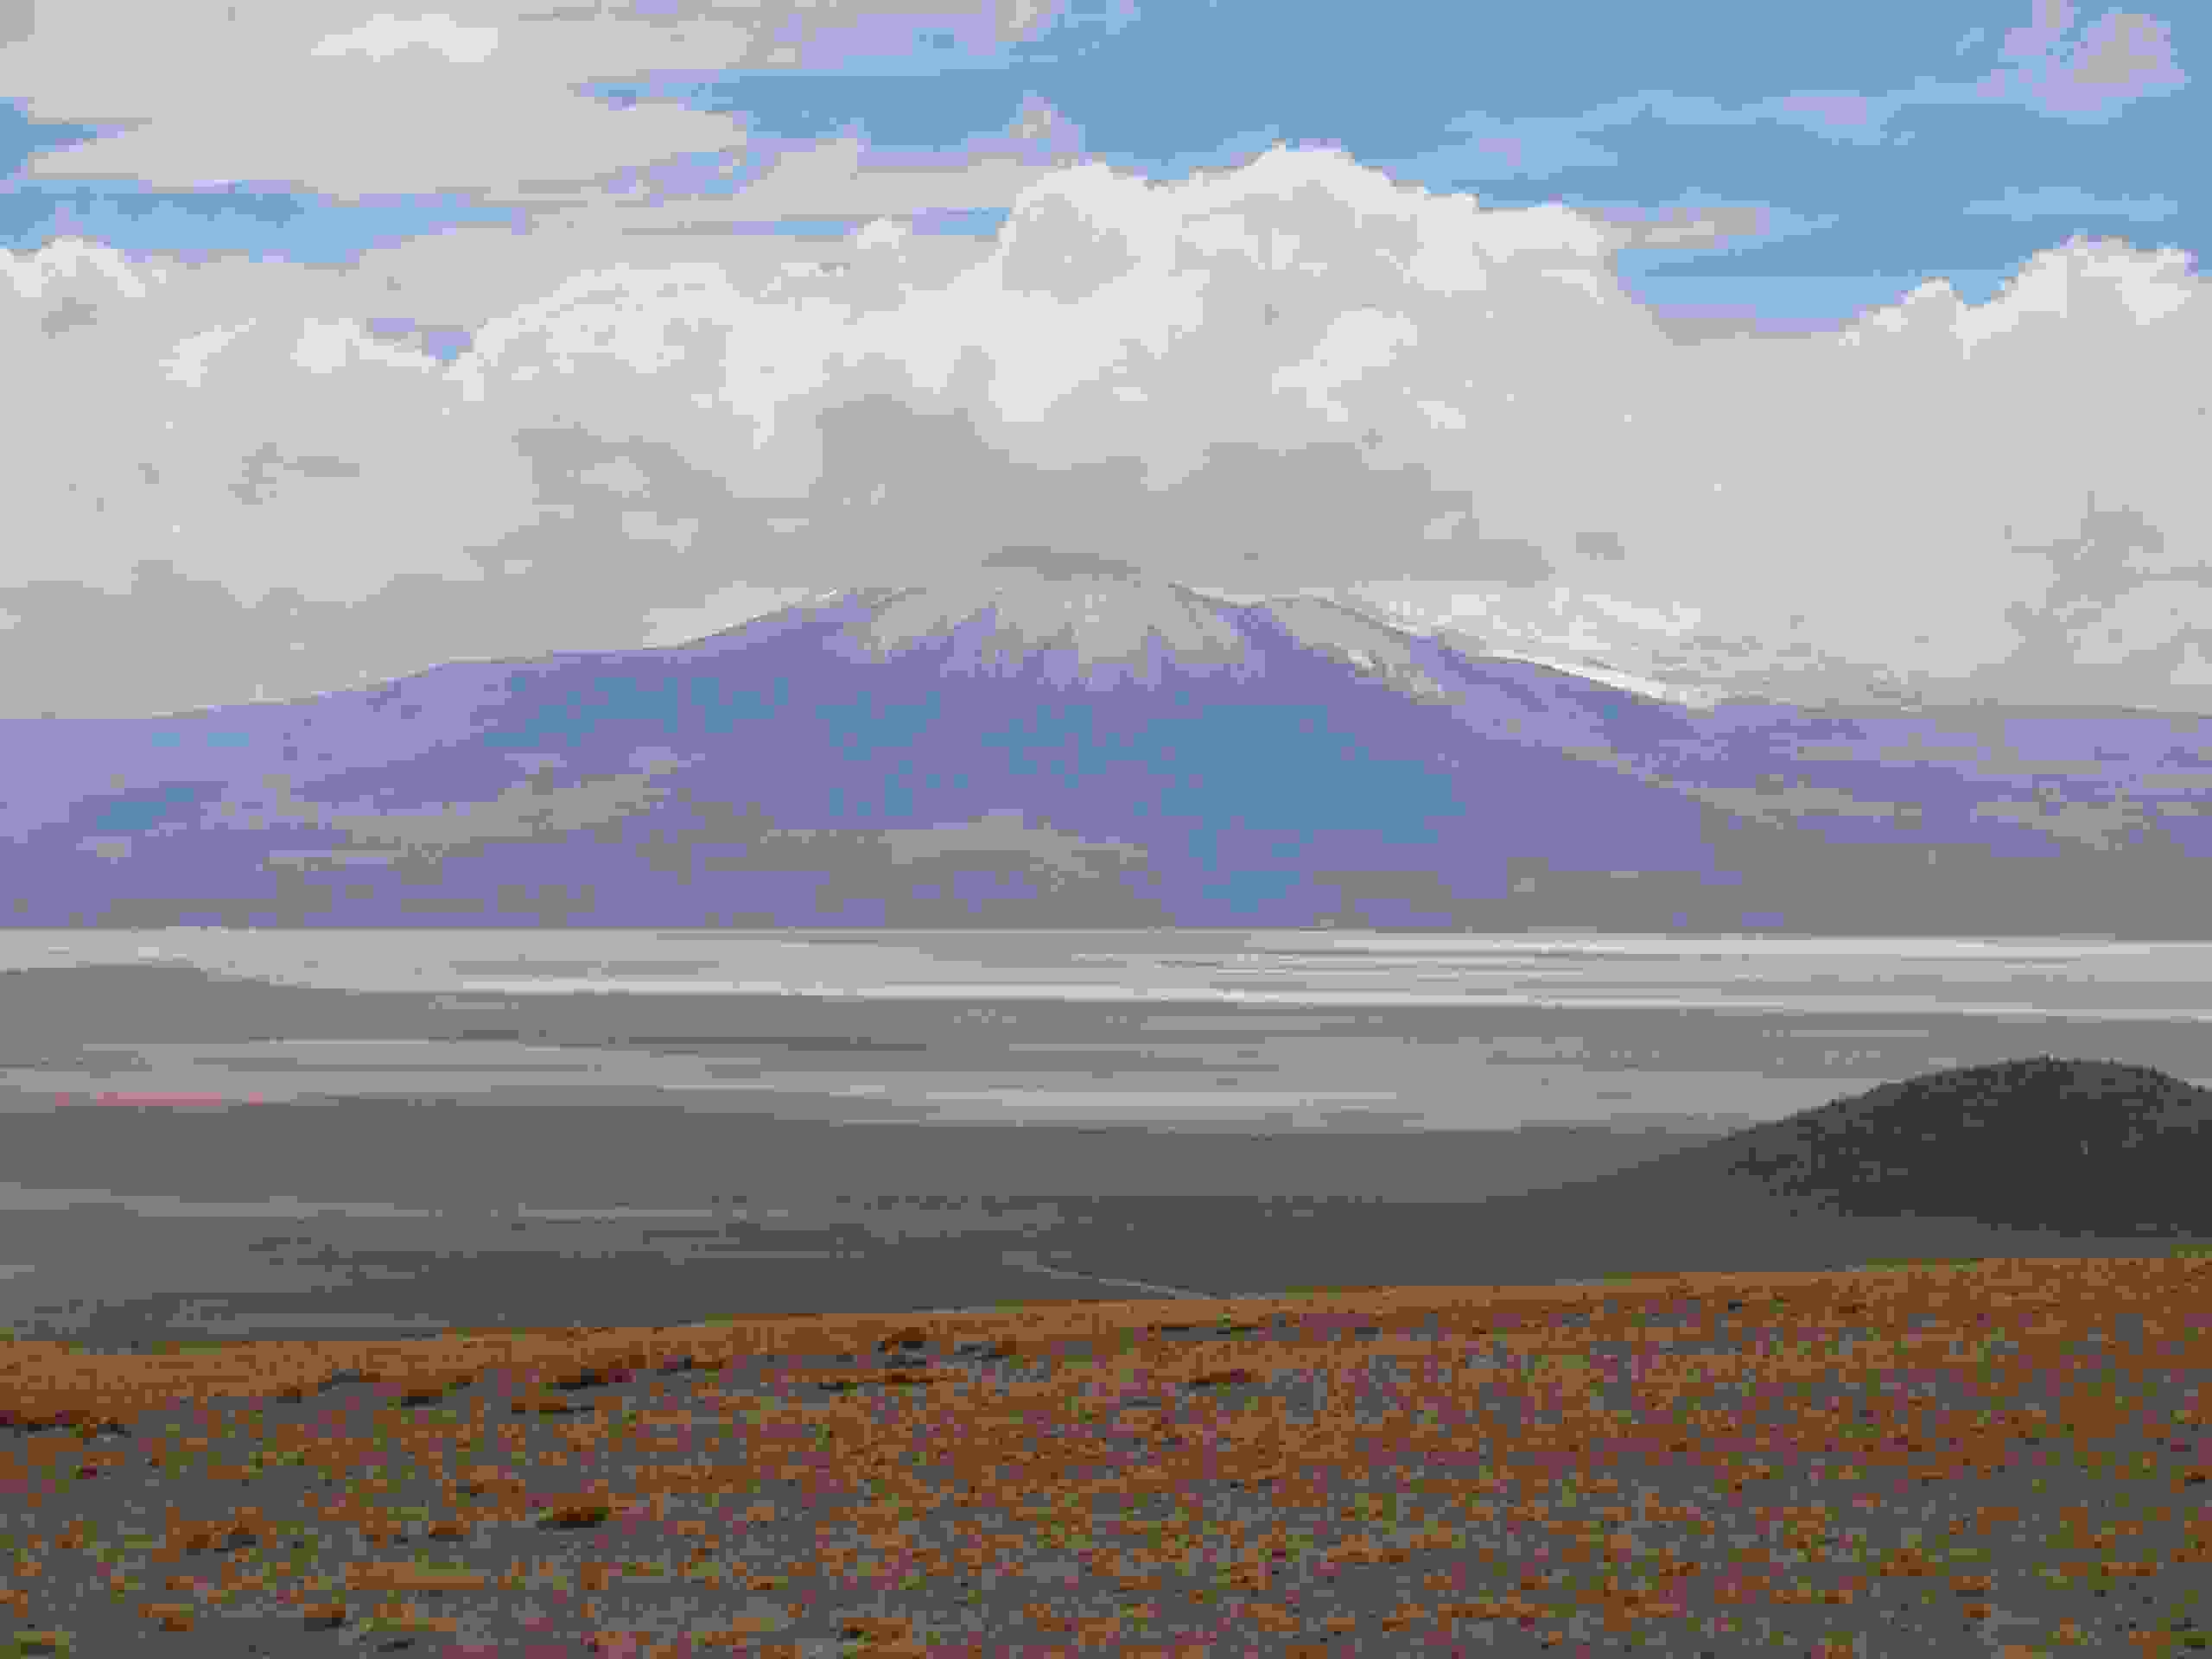
\includegraphics[width=\mywidth]{../wp-content/uploads/2015/04/wpid-wp-1427984819618.jpg} \end{center}

\pagebreak
 En plus du vent la pluie arrive, on s'arrête plus tôt que prévu dans un refuge et on reste dormir dans un dortoir.
\begin{center} 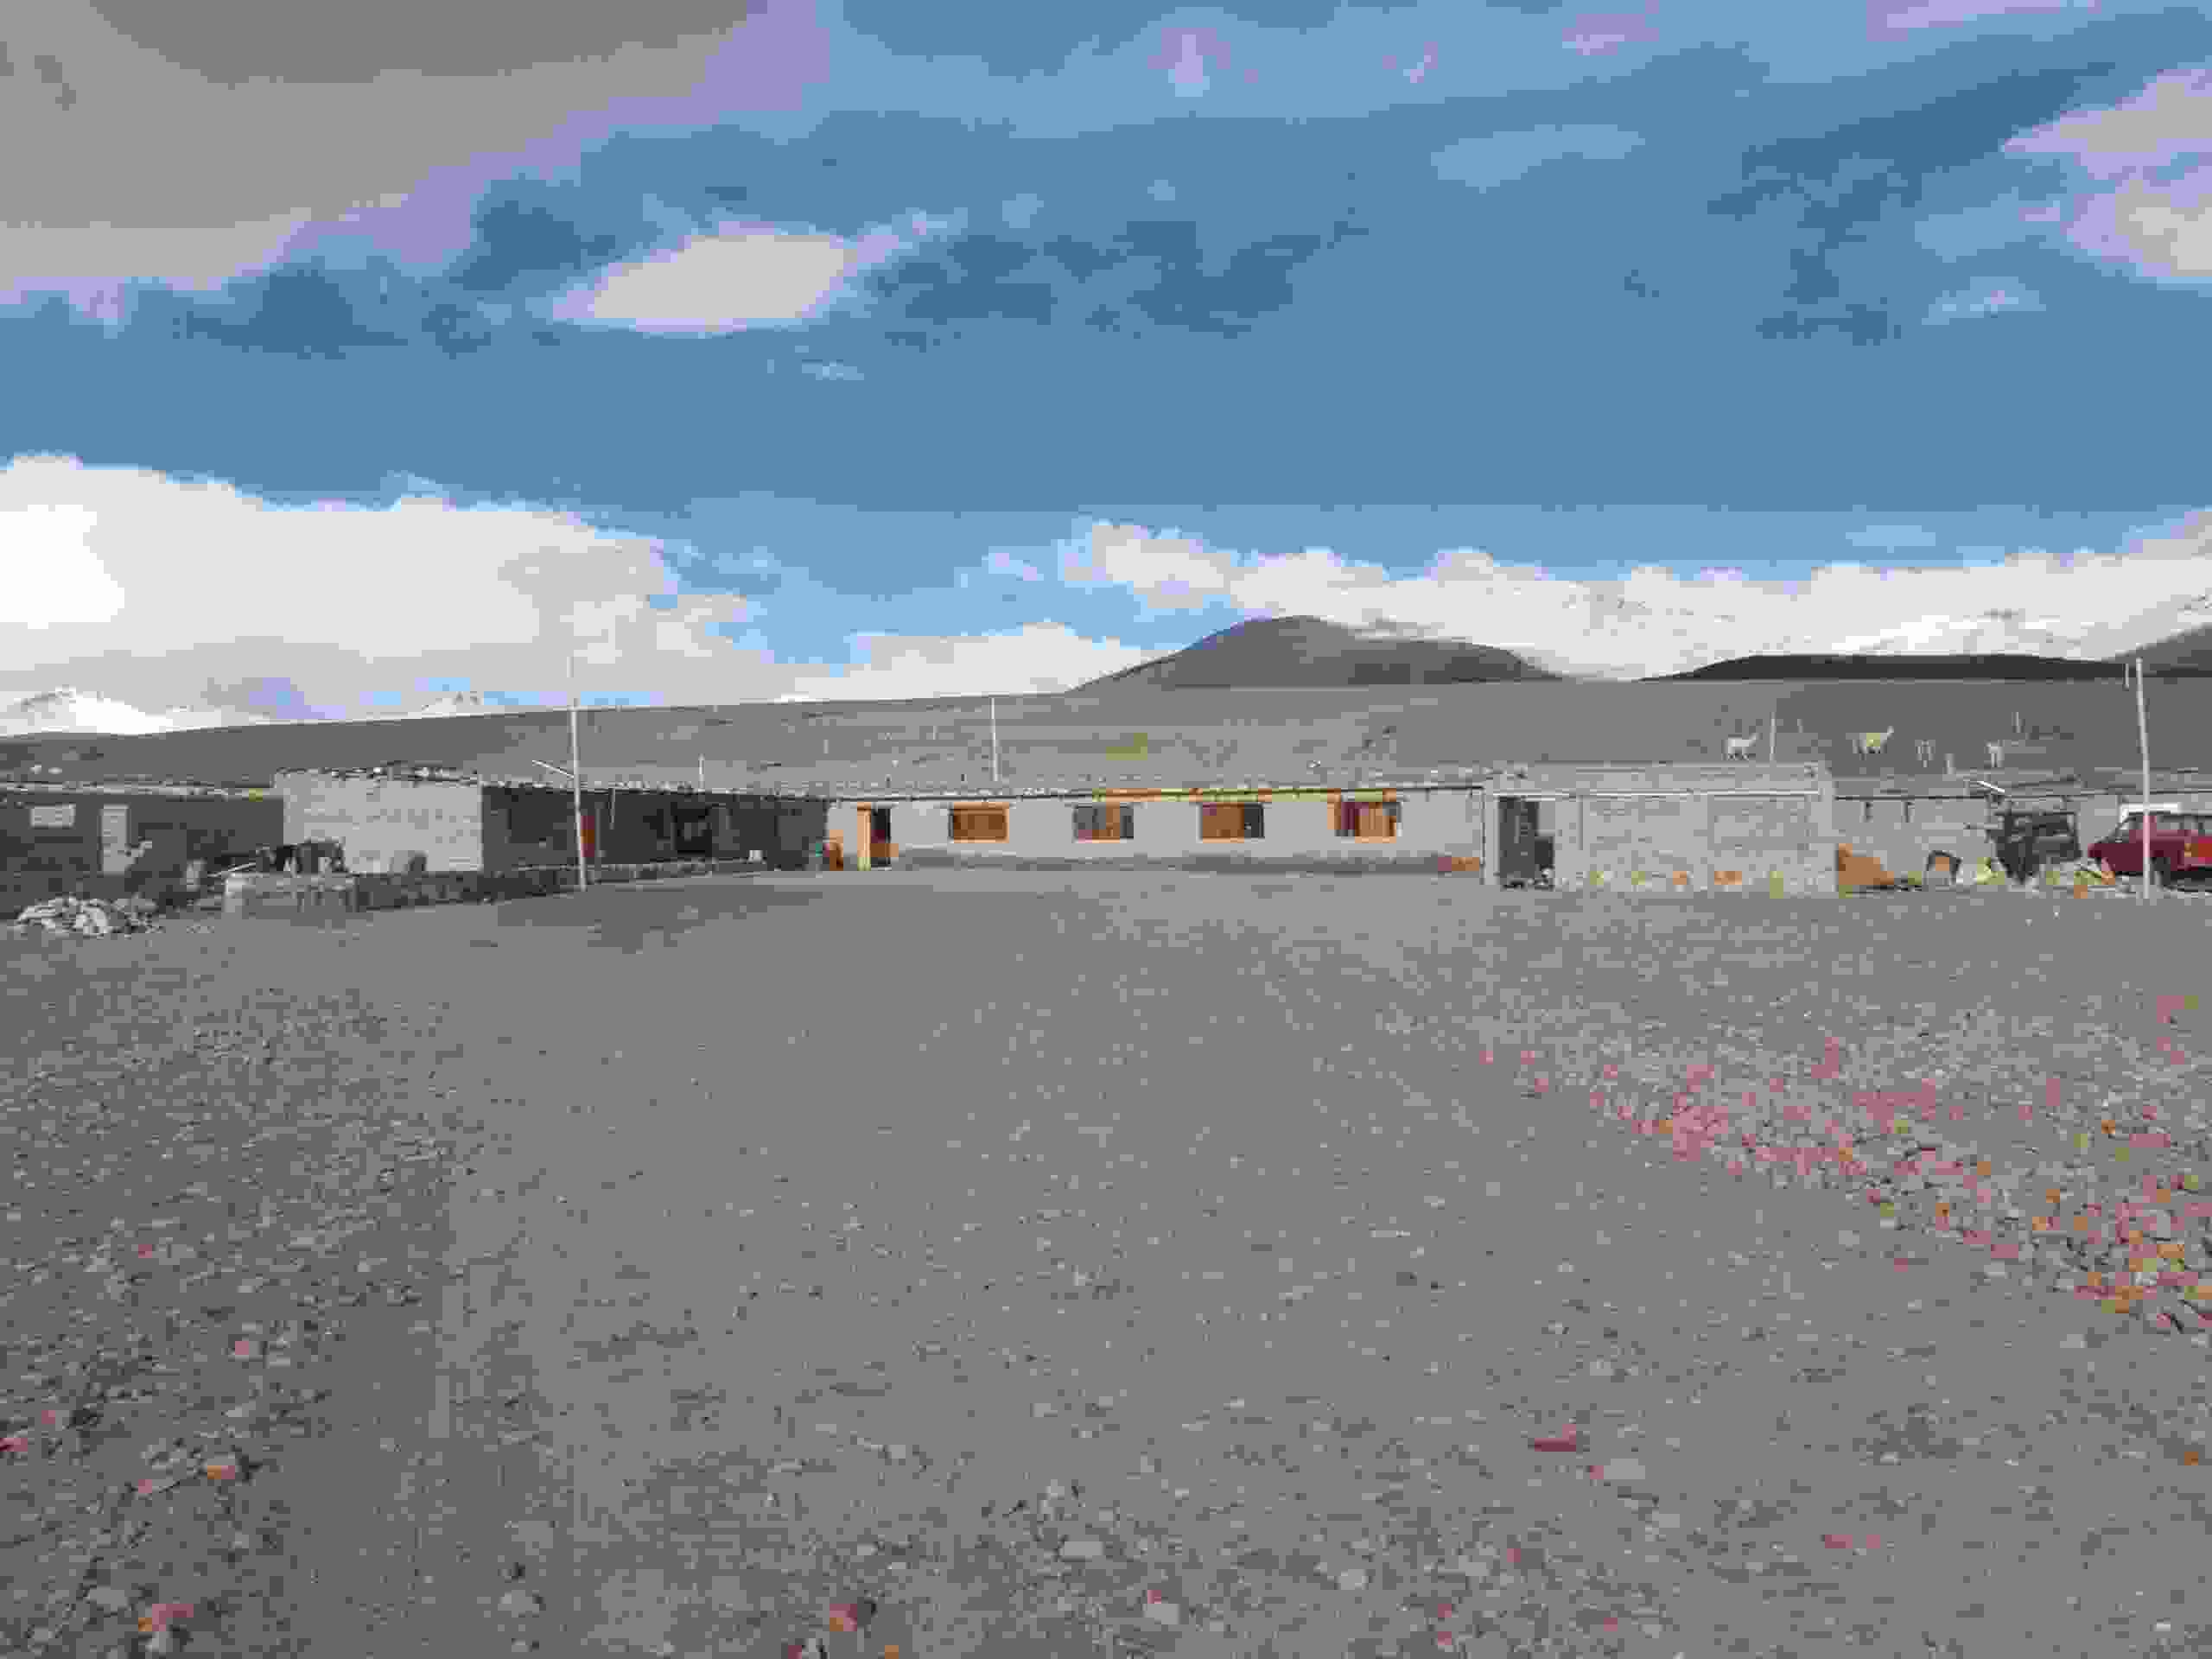
\includegraphics[width=\mywidth]{../wp-content/uploads/2015/04/wpid-wp-1427984897297.jpg} \end{center}

 \subsection*{5\ieme\ jour} 

 10km dans le sable pour arriver au ravitaillement : on s'est fait déposer un carton de nourriture dans un refuge.
\begin{center} 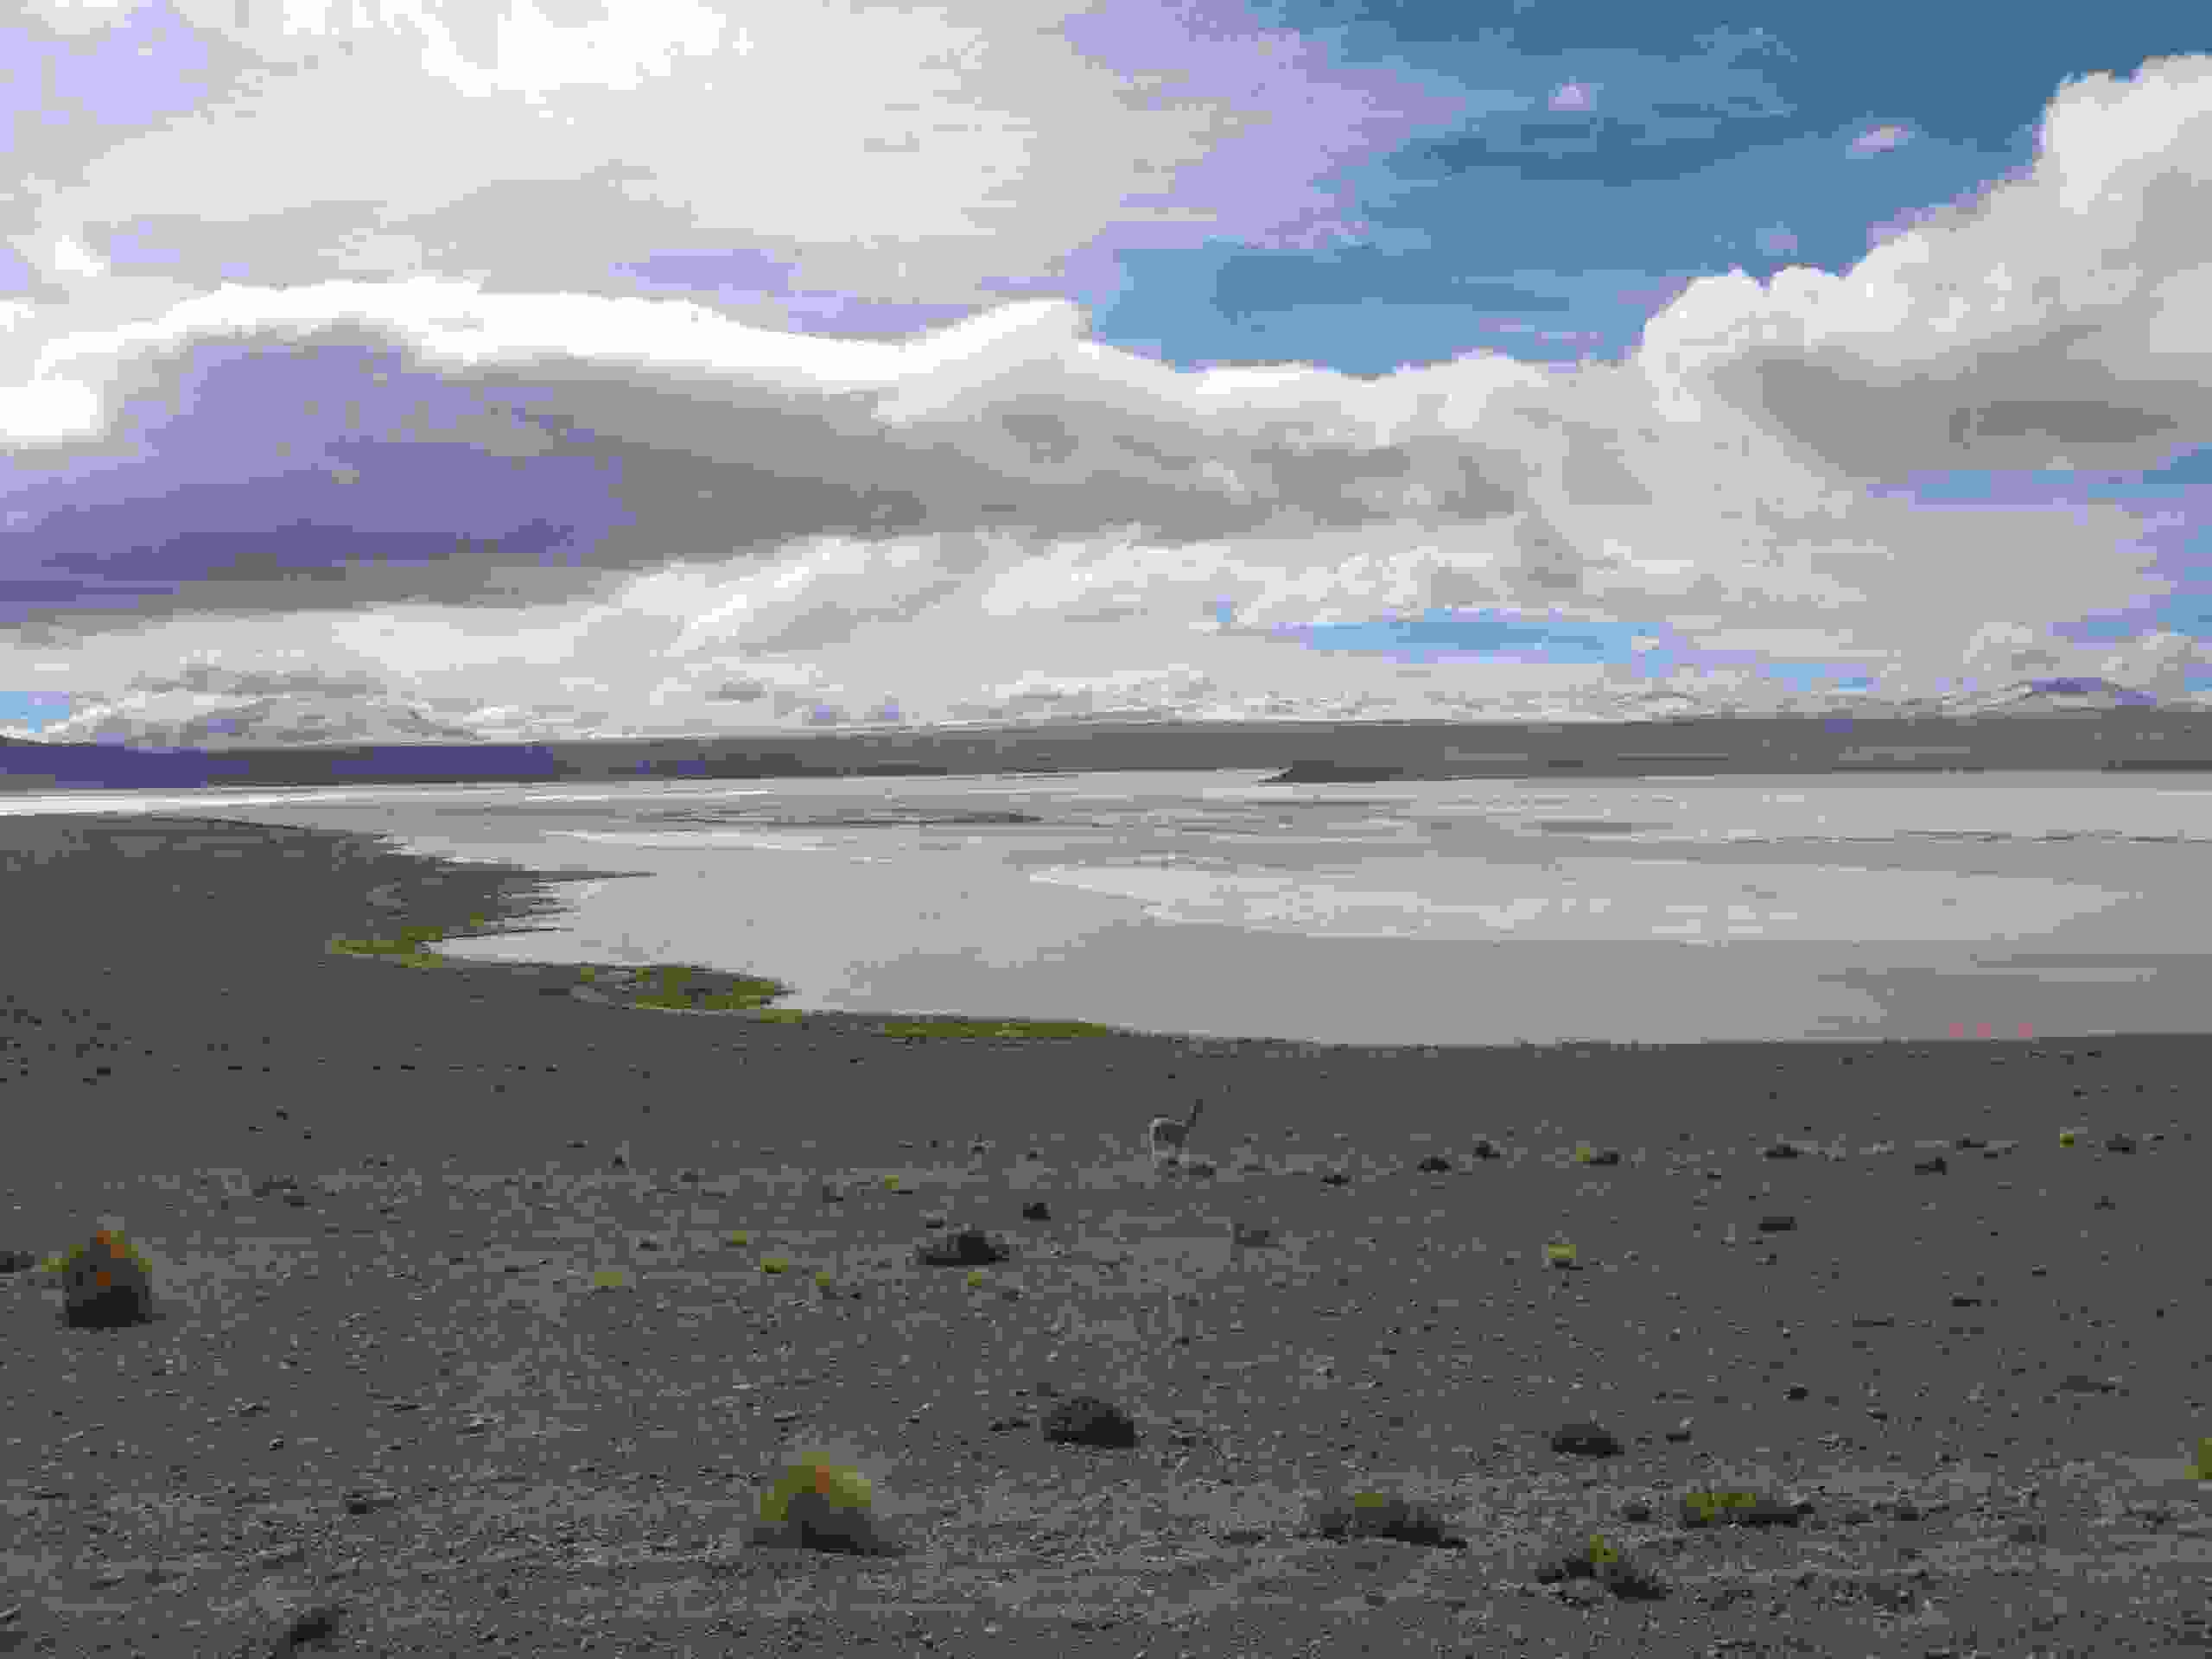
\includegraphics[width=\mywidth]{../wp-content/uploads/2015/04/wpid-wp-1427984947015.jpg} \end{center}

 Ça continue à monter avec le vent de face.
\begin{center} 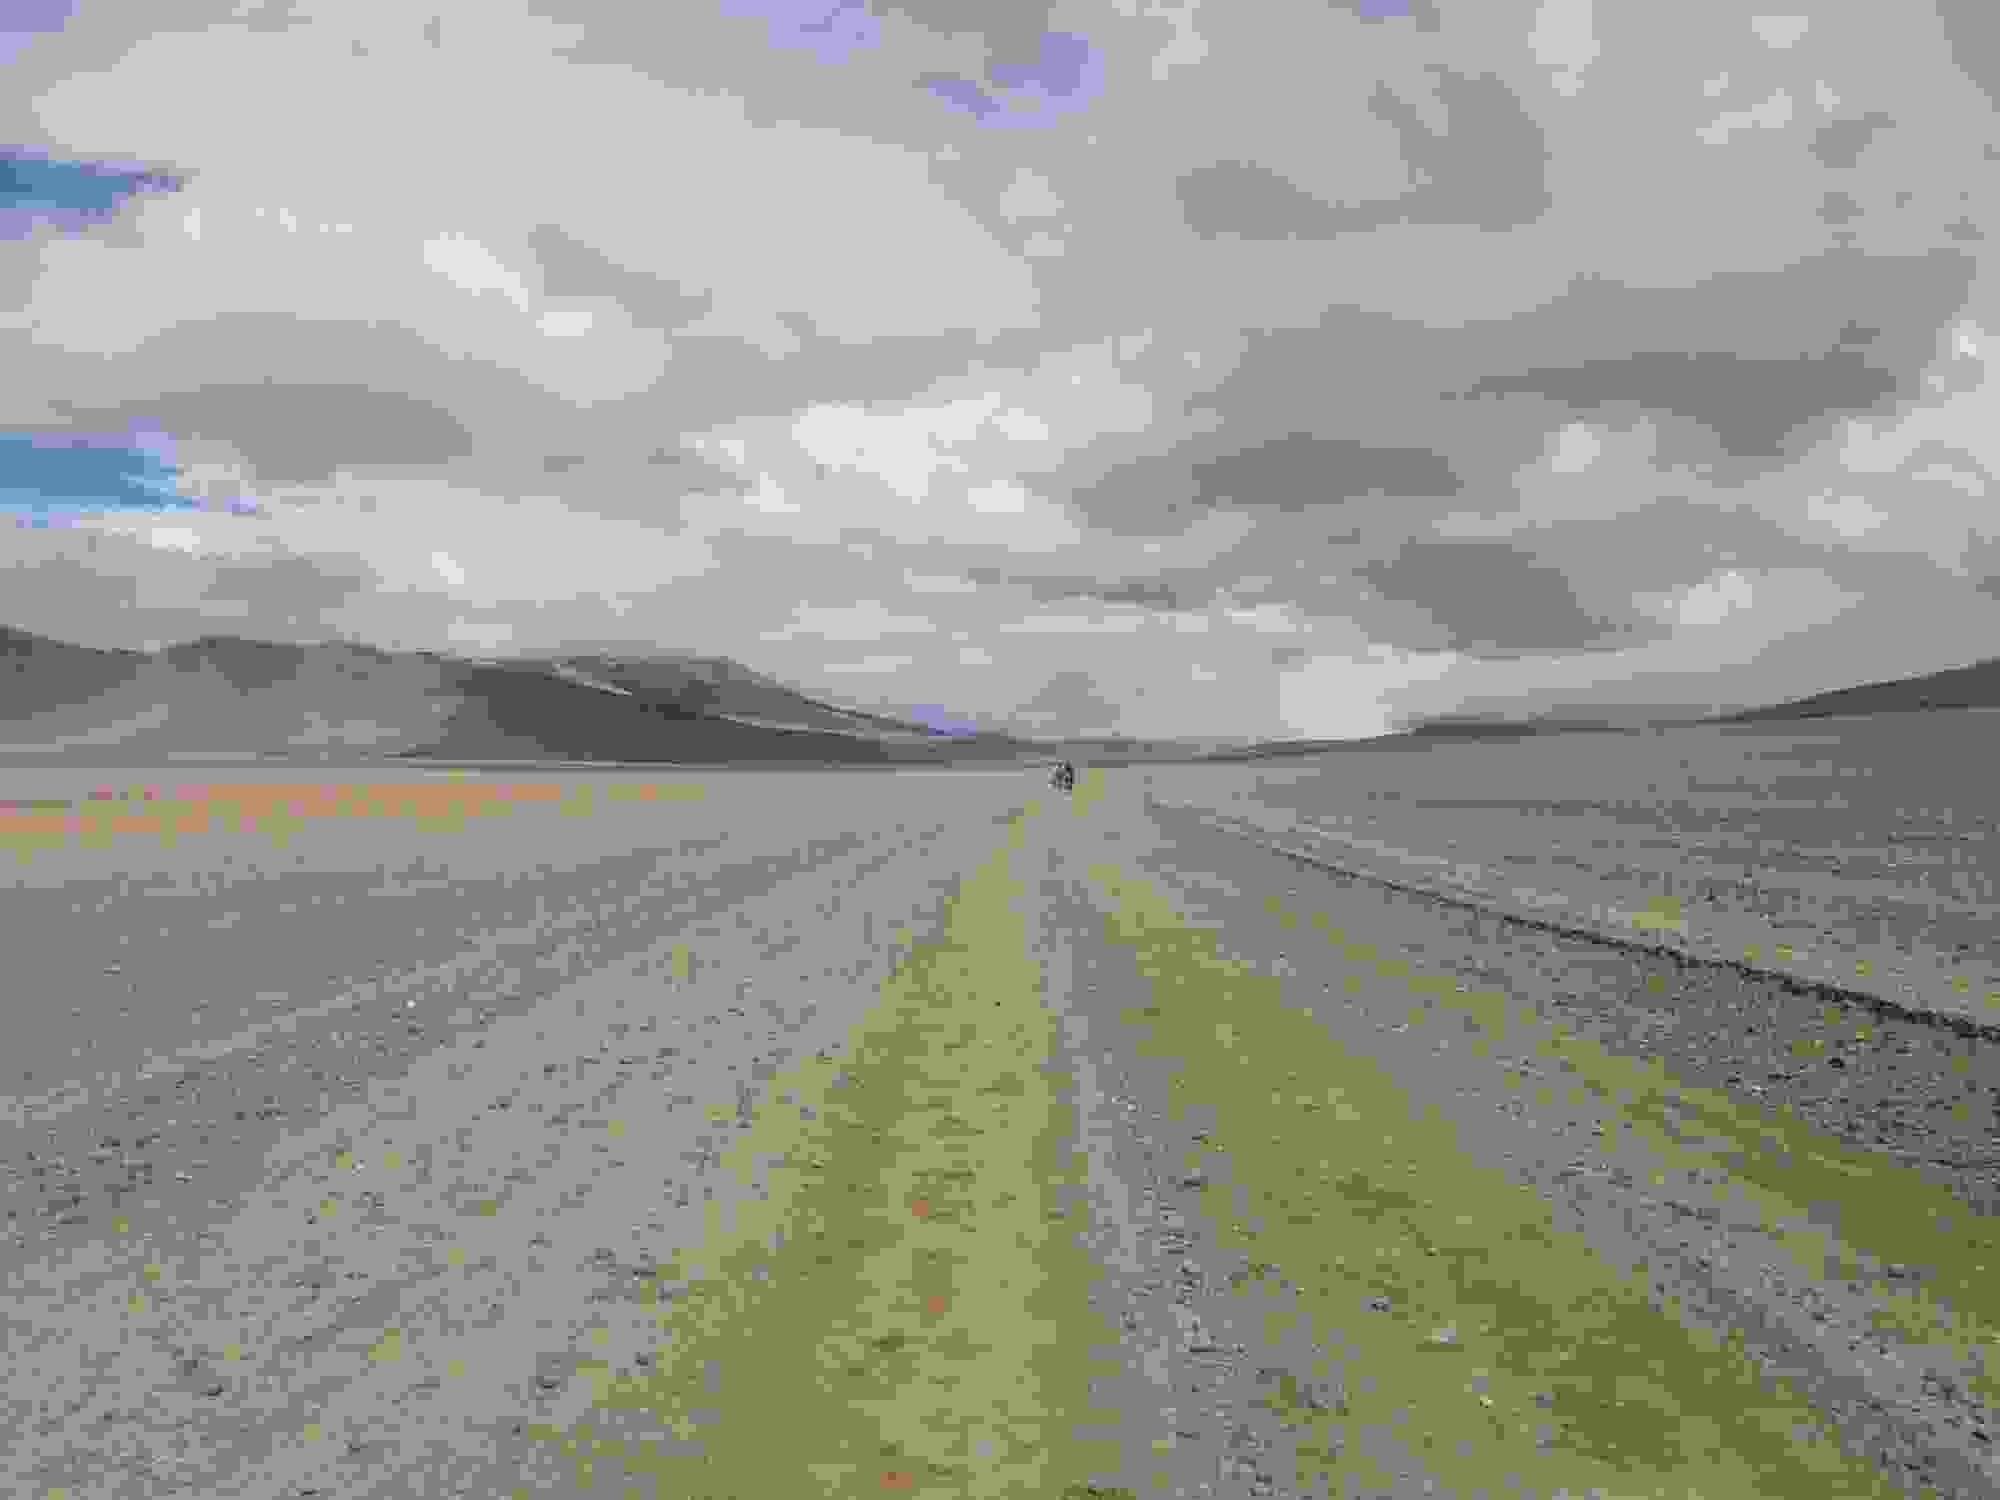
\includegraphics[width=\mywidth]{../wp-content/uploads/2015/04/wpid-wp-1427988827948.jpg} \end{center}

  Petit passage sous la grêle et on arrive enfin à l'Arbol de Piedra.
\begin{center} 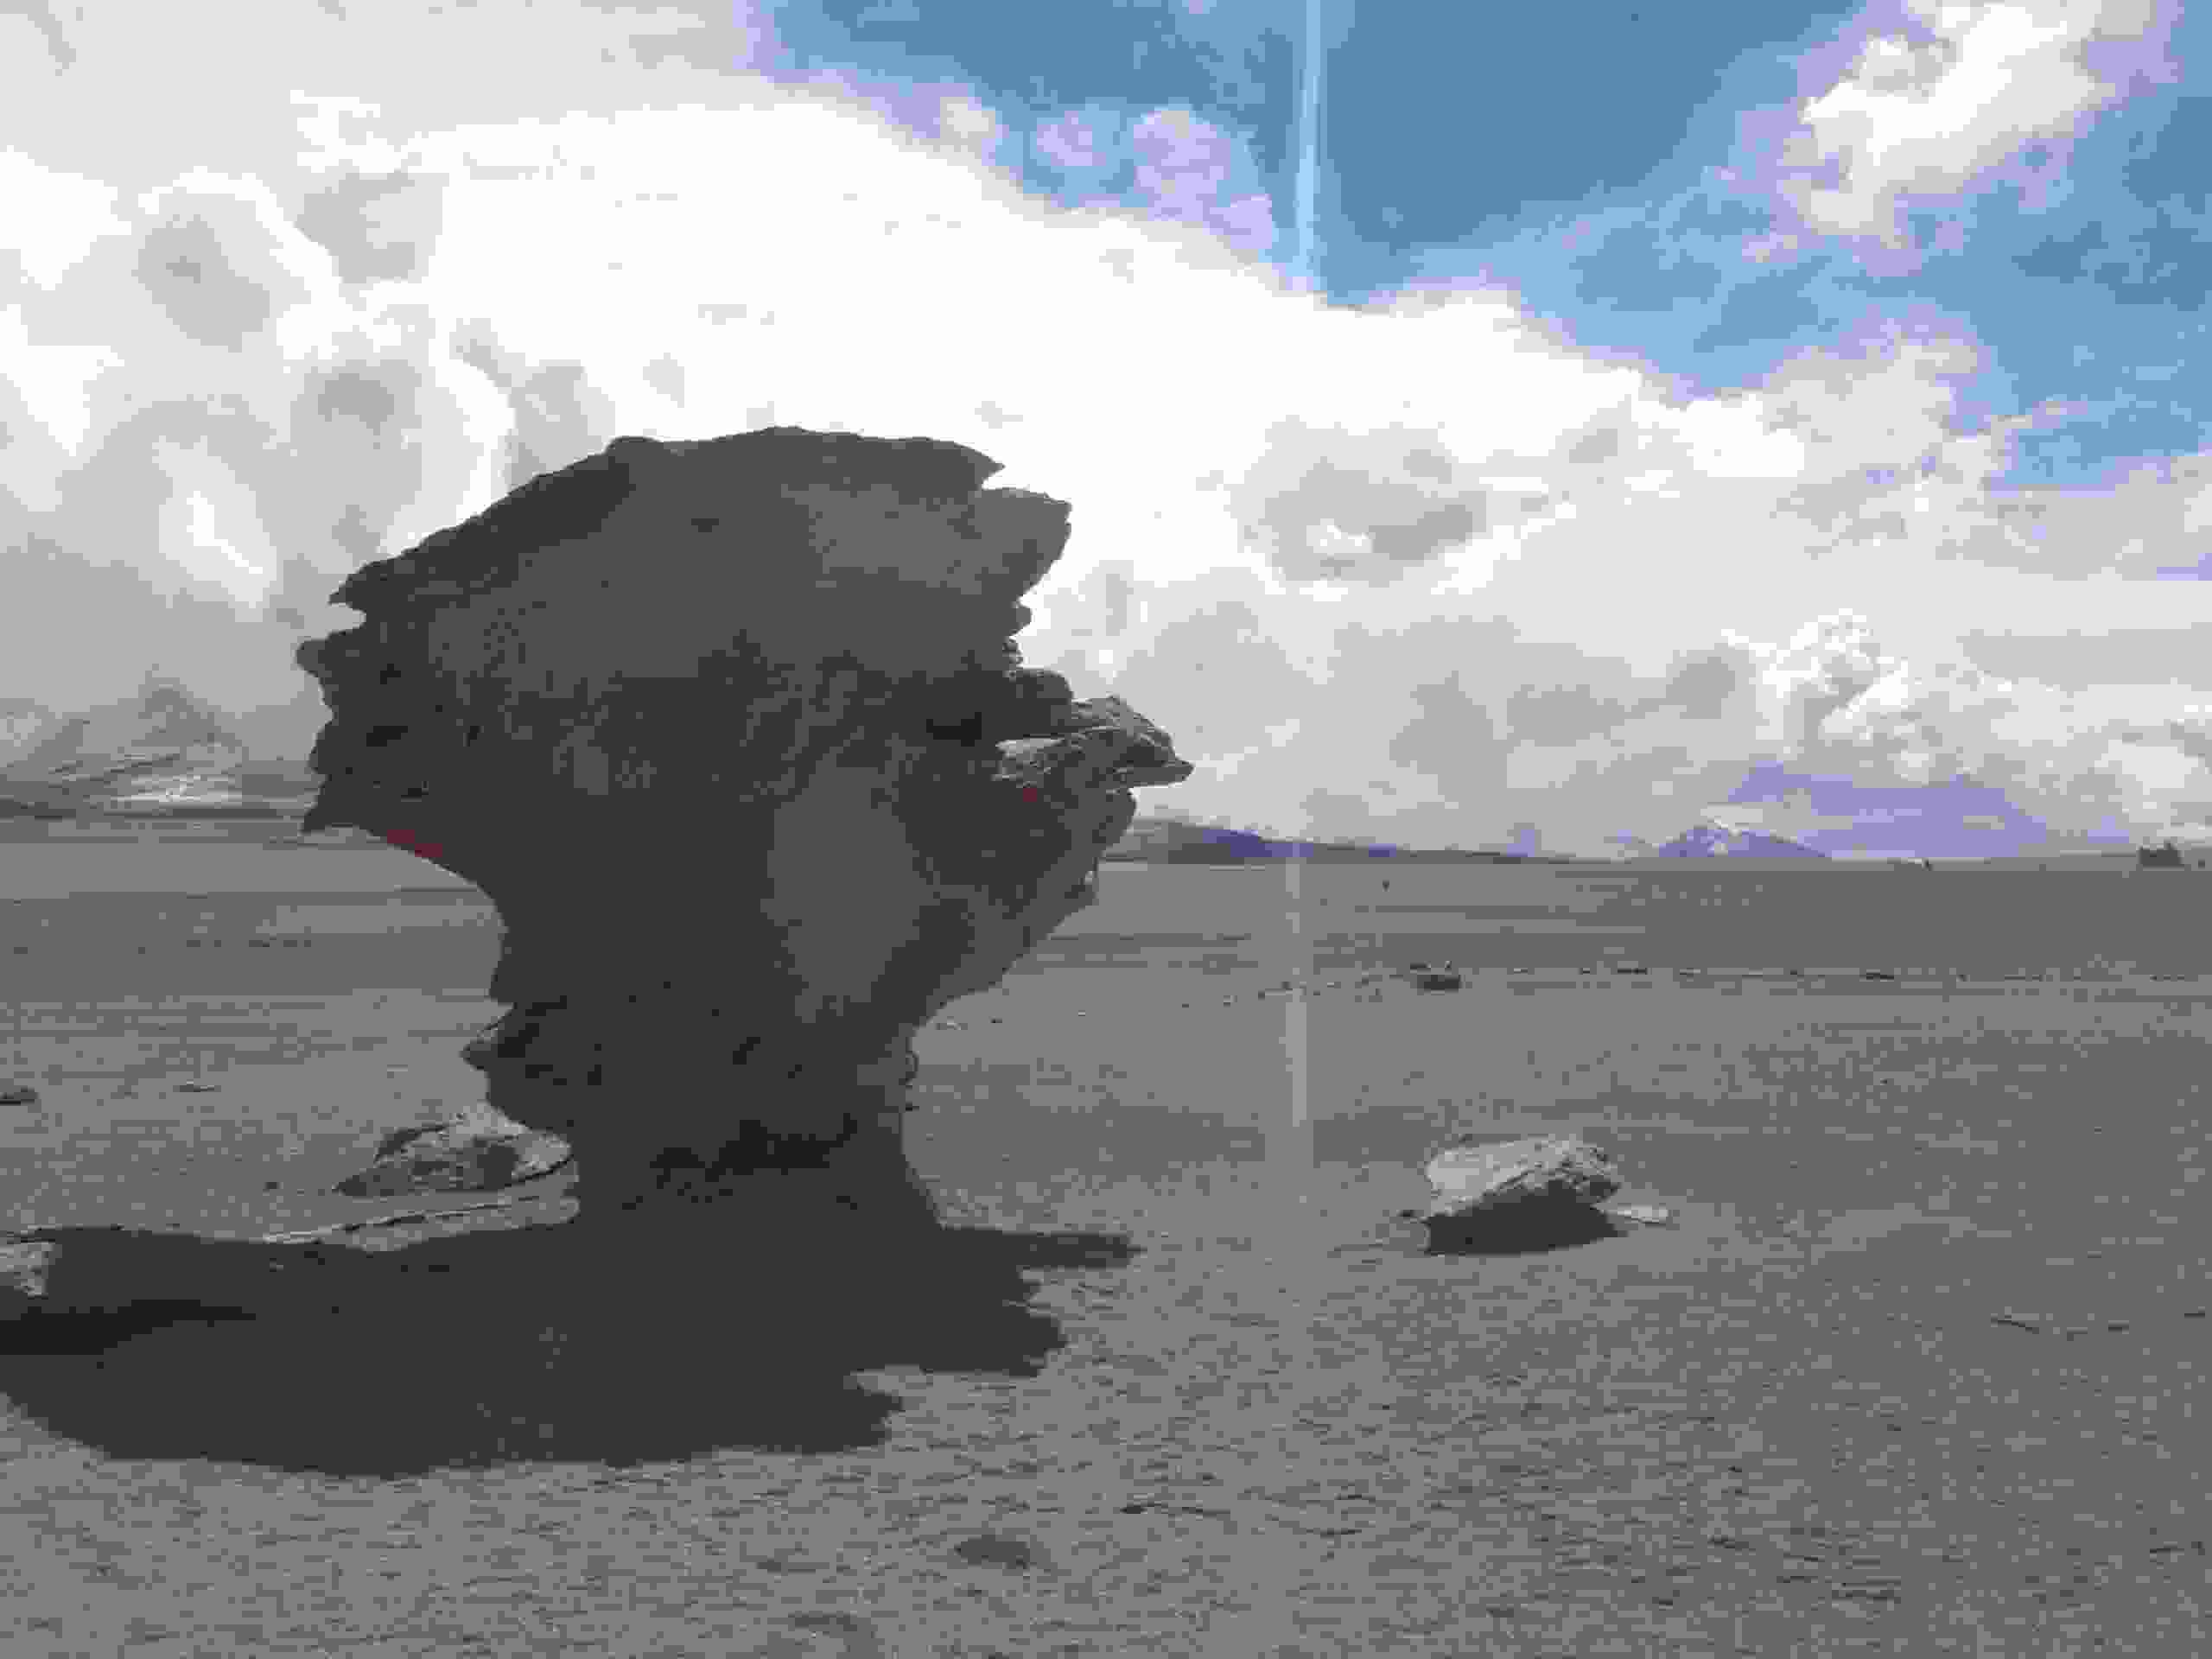
\includegraphics[width=\mywidth]{../wp-content/uploads/2015/04/wpid-wp-1427985000520.jpg} \end{center}
\begin{center} 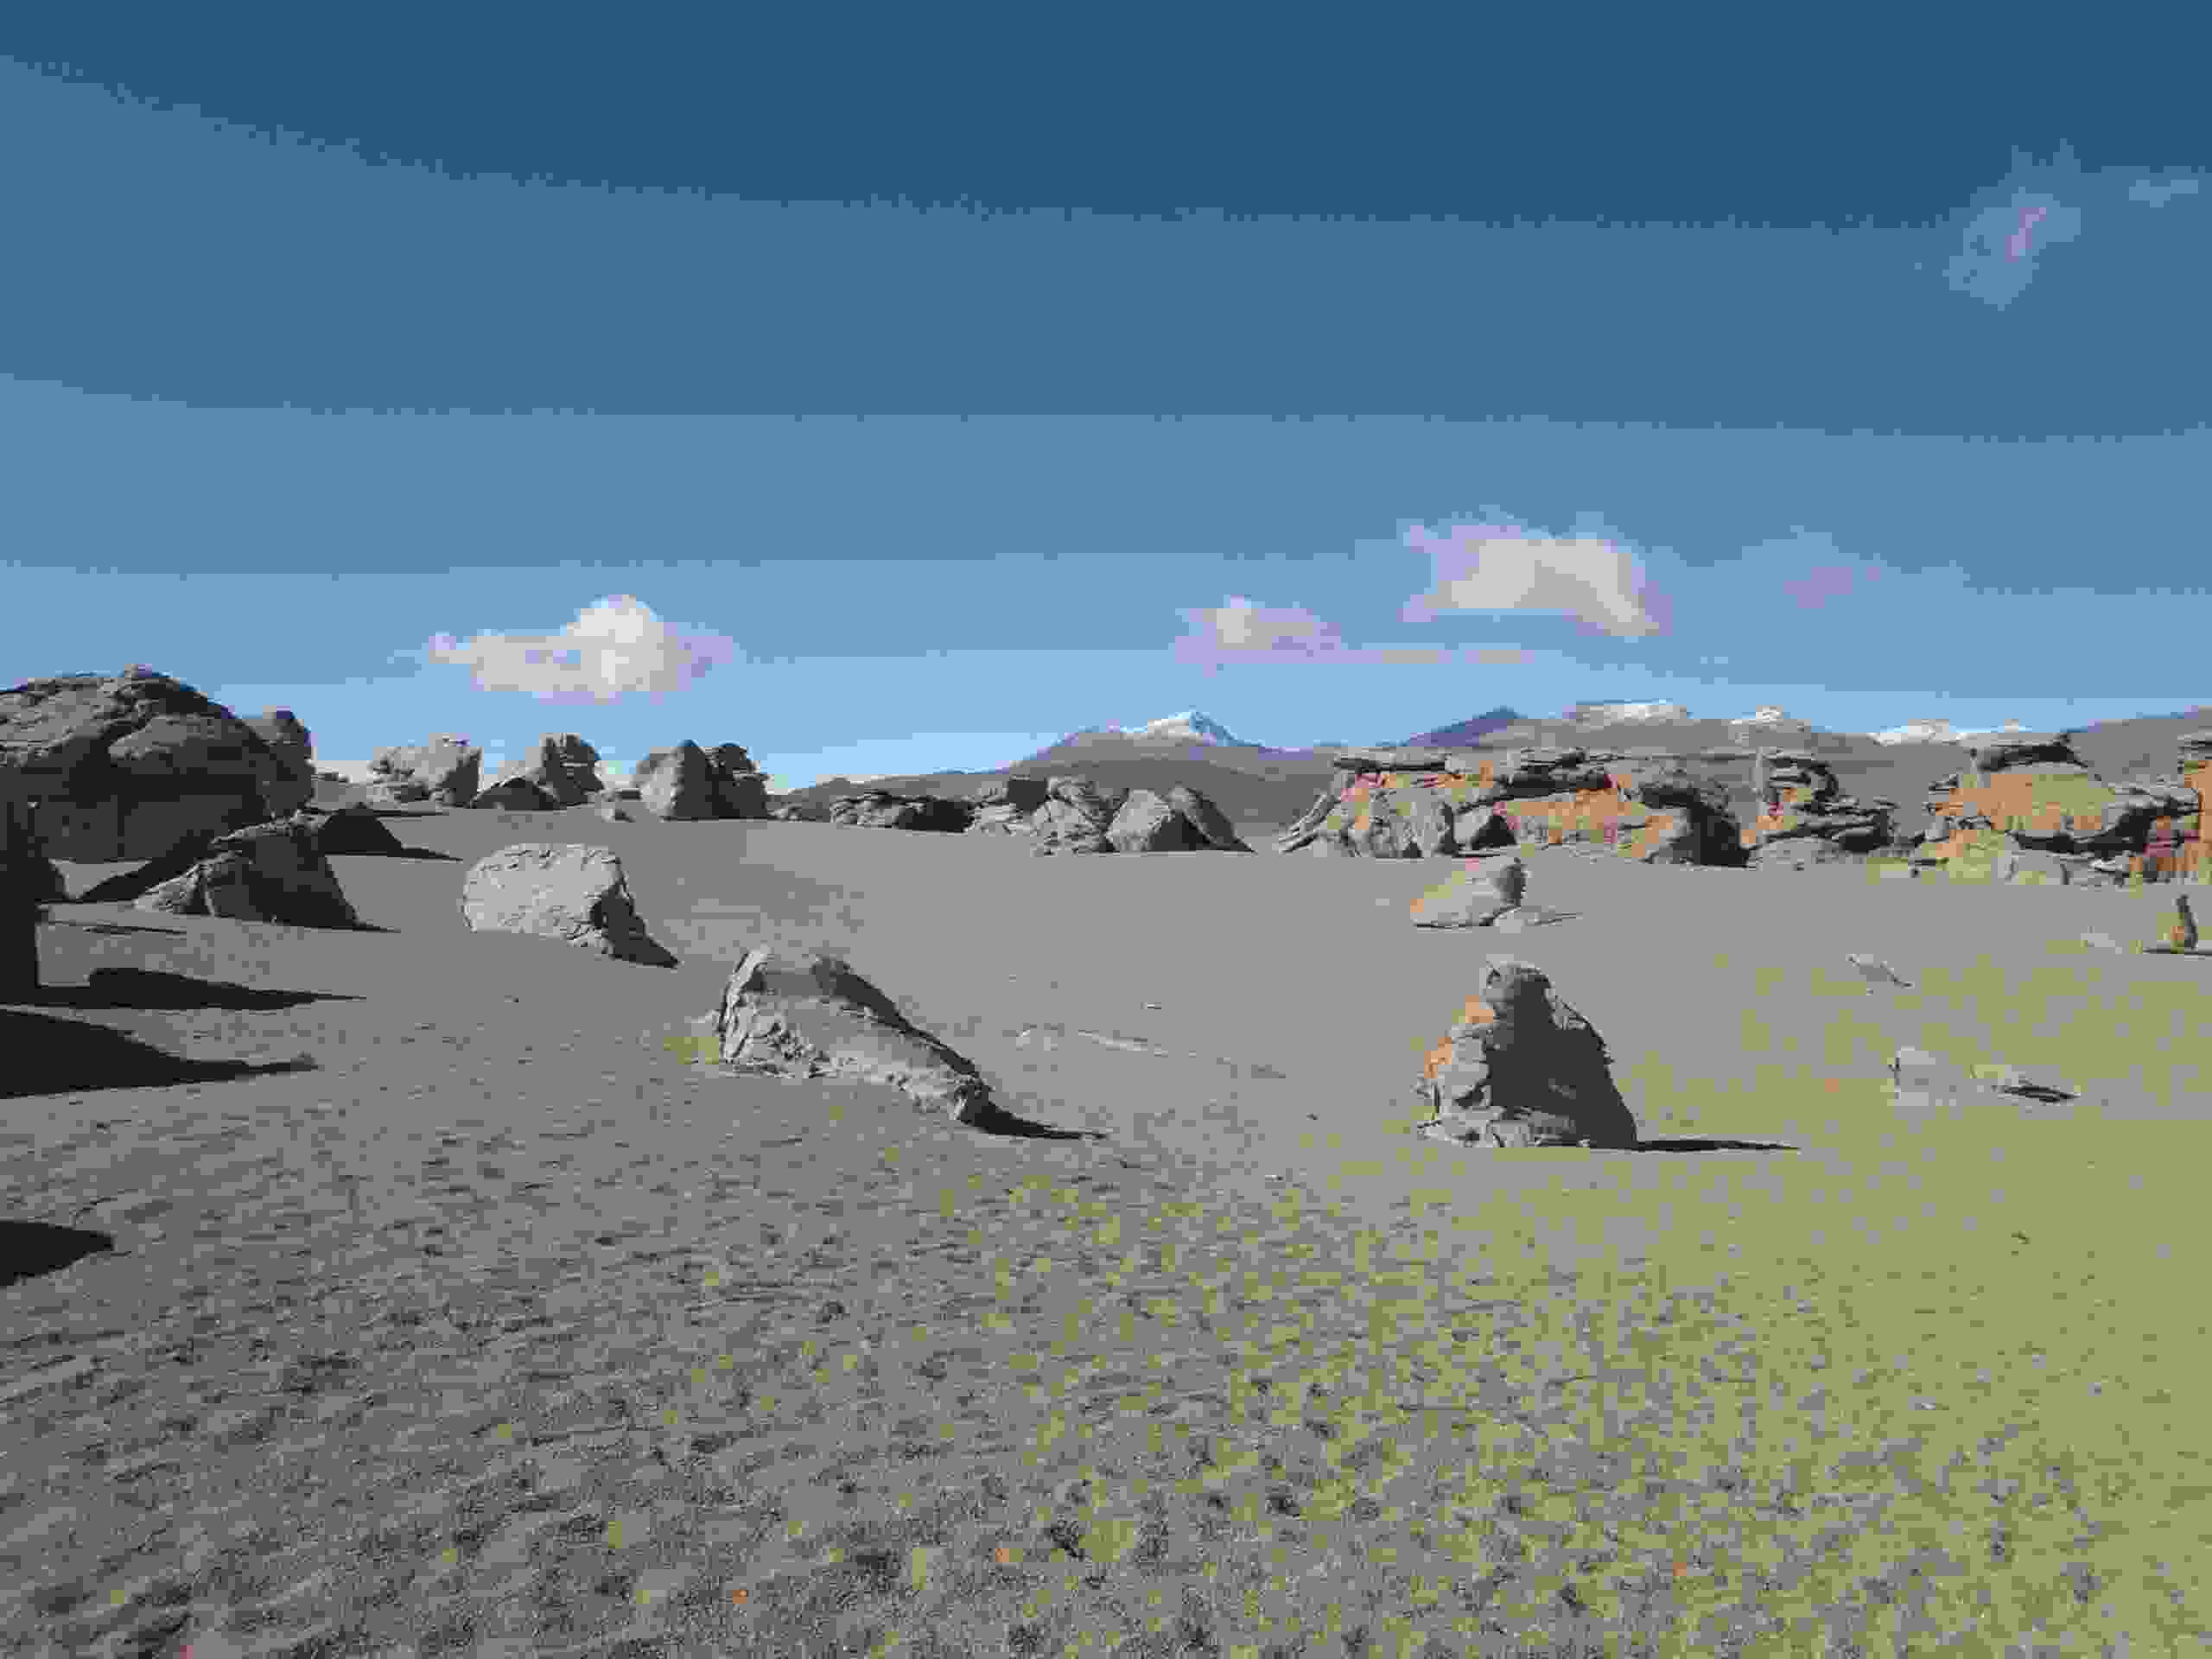
\includegraphics[width=\mywidth]{../wp-content/uploads/2015/04/wpid-wp-1427985029857.jpg} \end{center}

 Bivouac très froid à 4600m.
\begin{center} 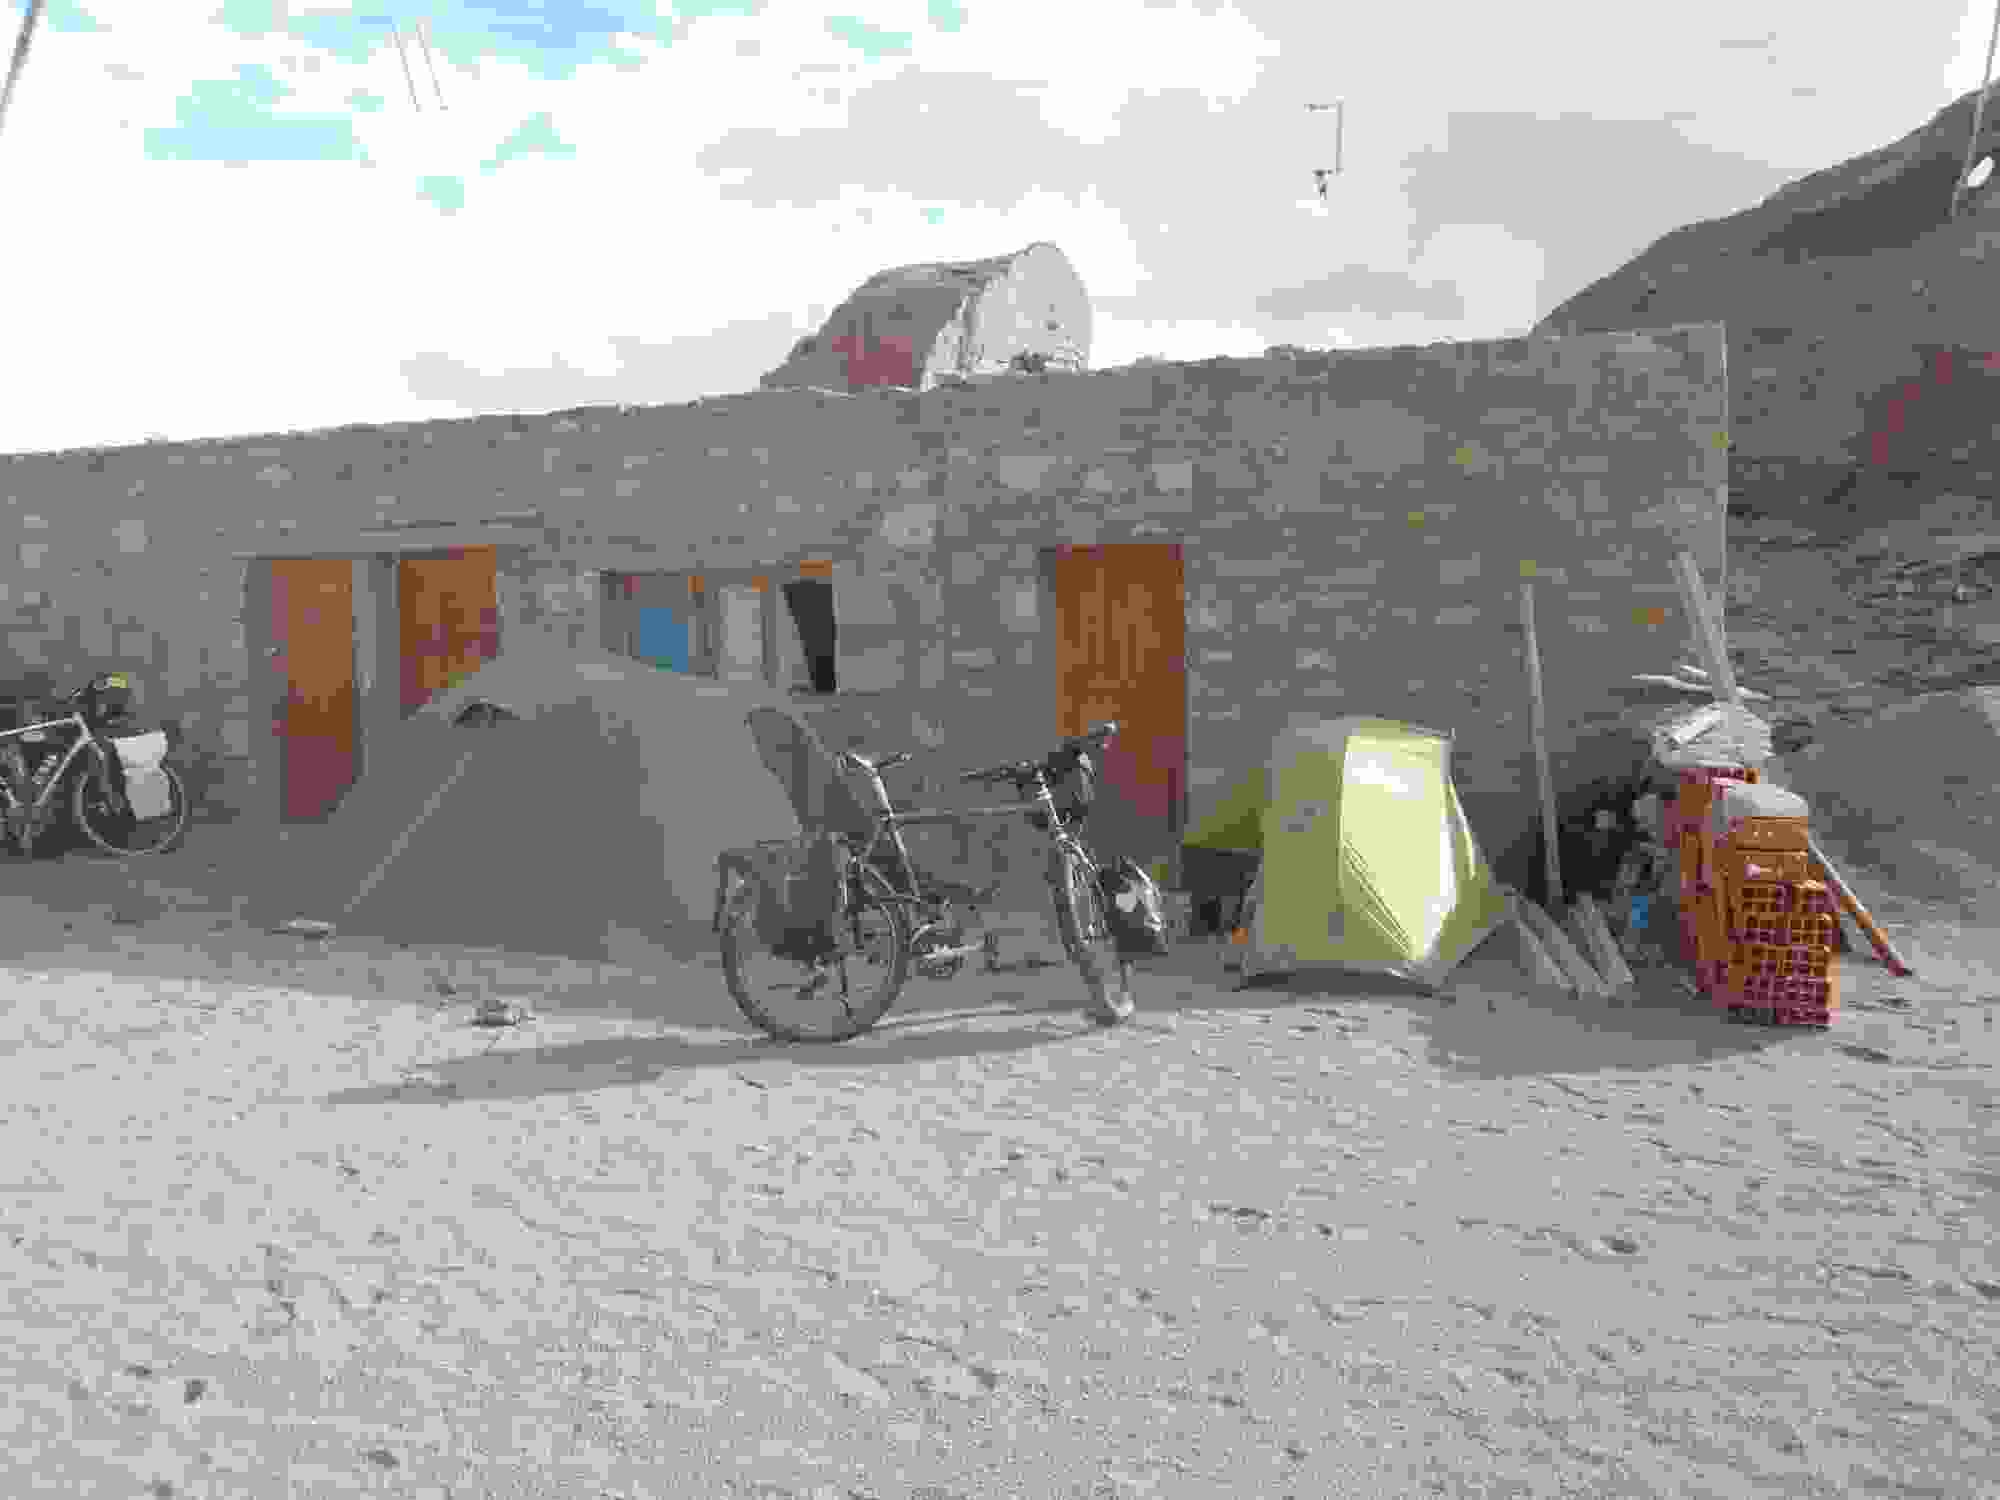
\includegraphics[width=\mywidth]{../wp-content/uploads/2015/04/wpid-wp-1427988855397.jpg} \end{center}

\pagebreak
 \subsection*{6\ieme\ jour} 
 Le temps s'améliore mais toujours le vent de face.
\begin{center} 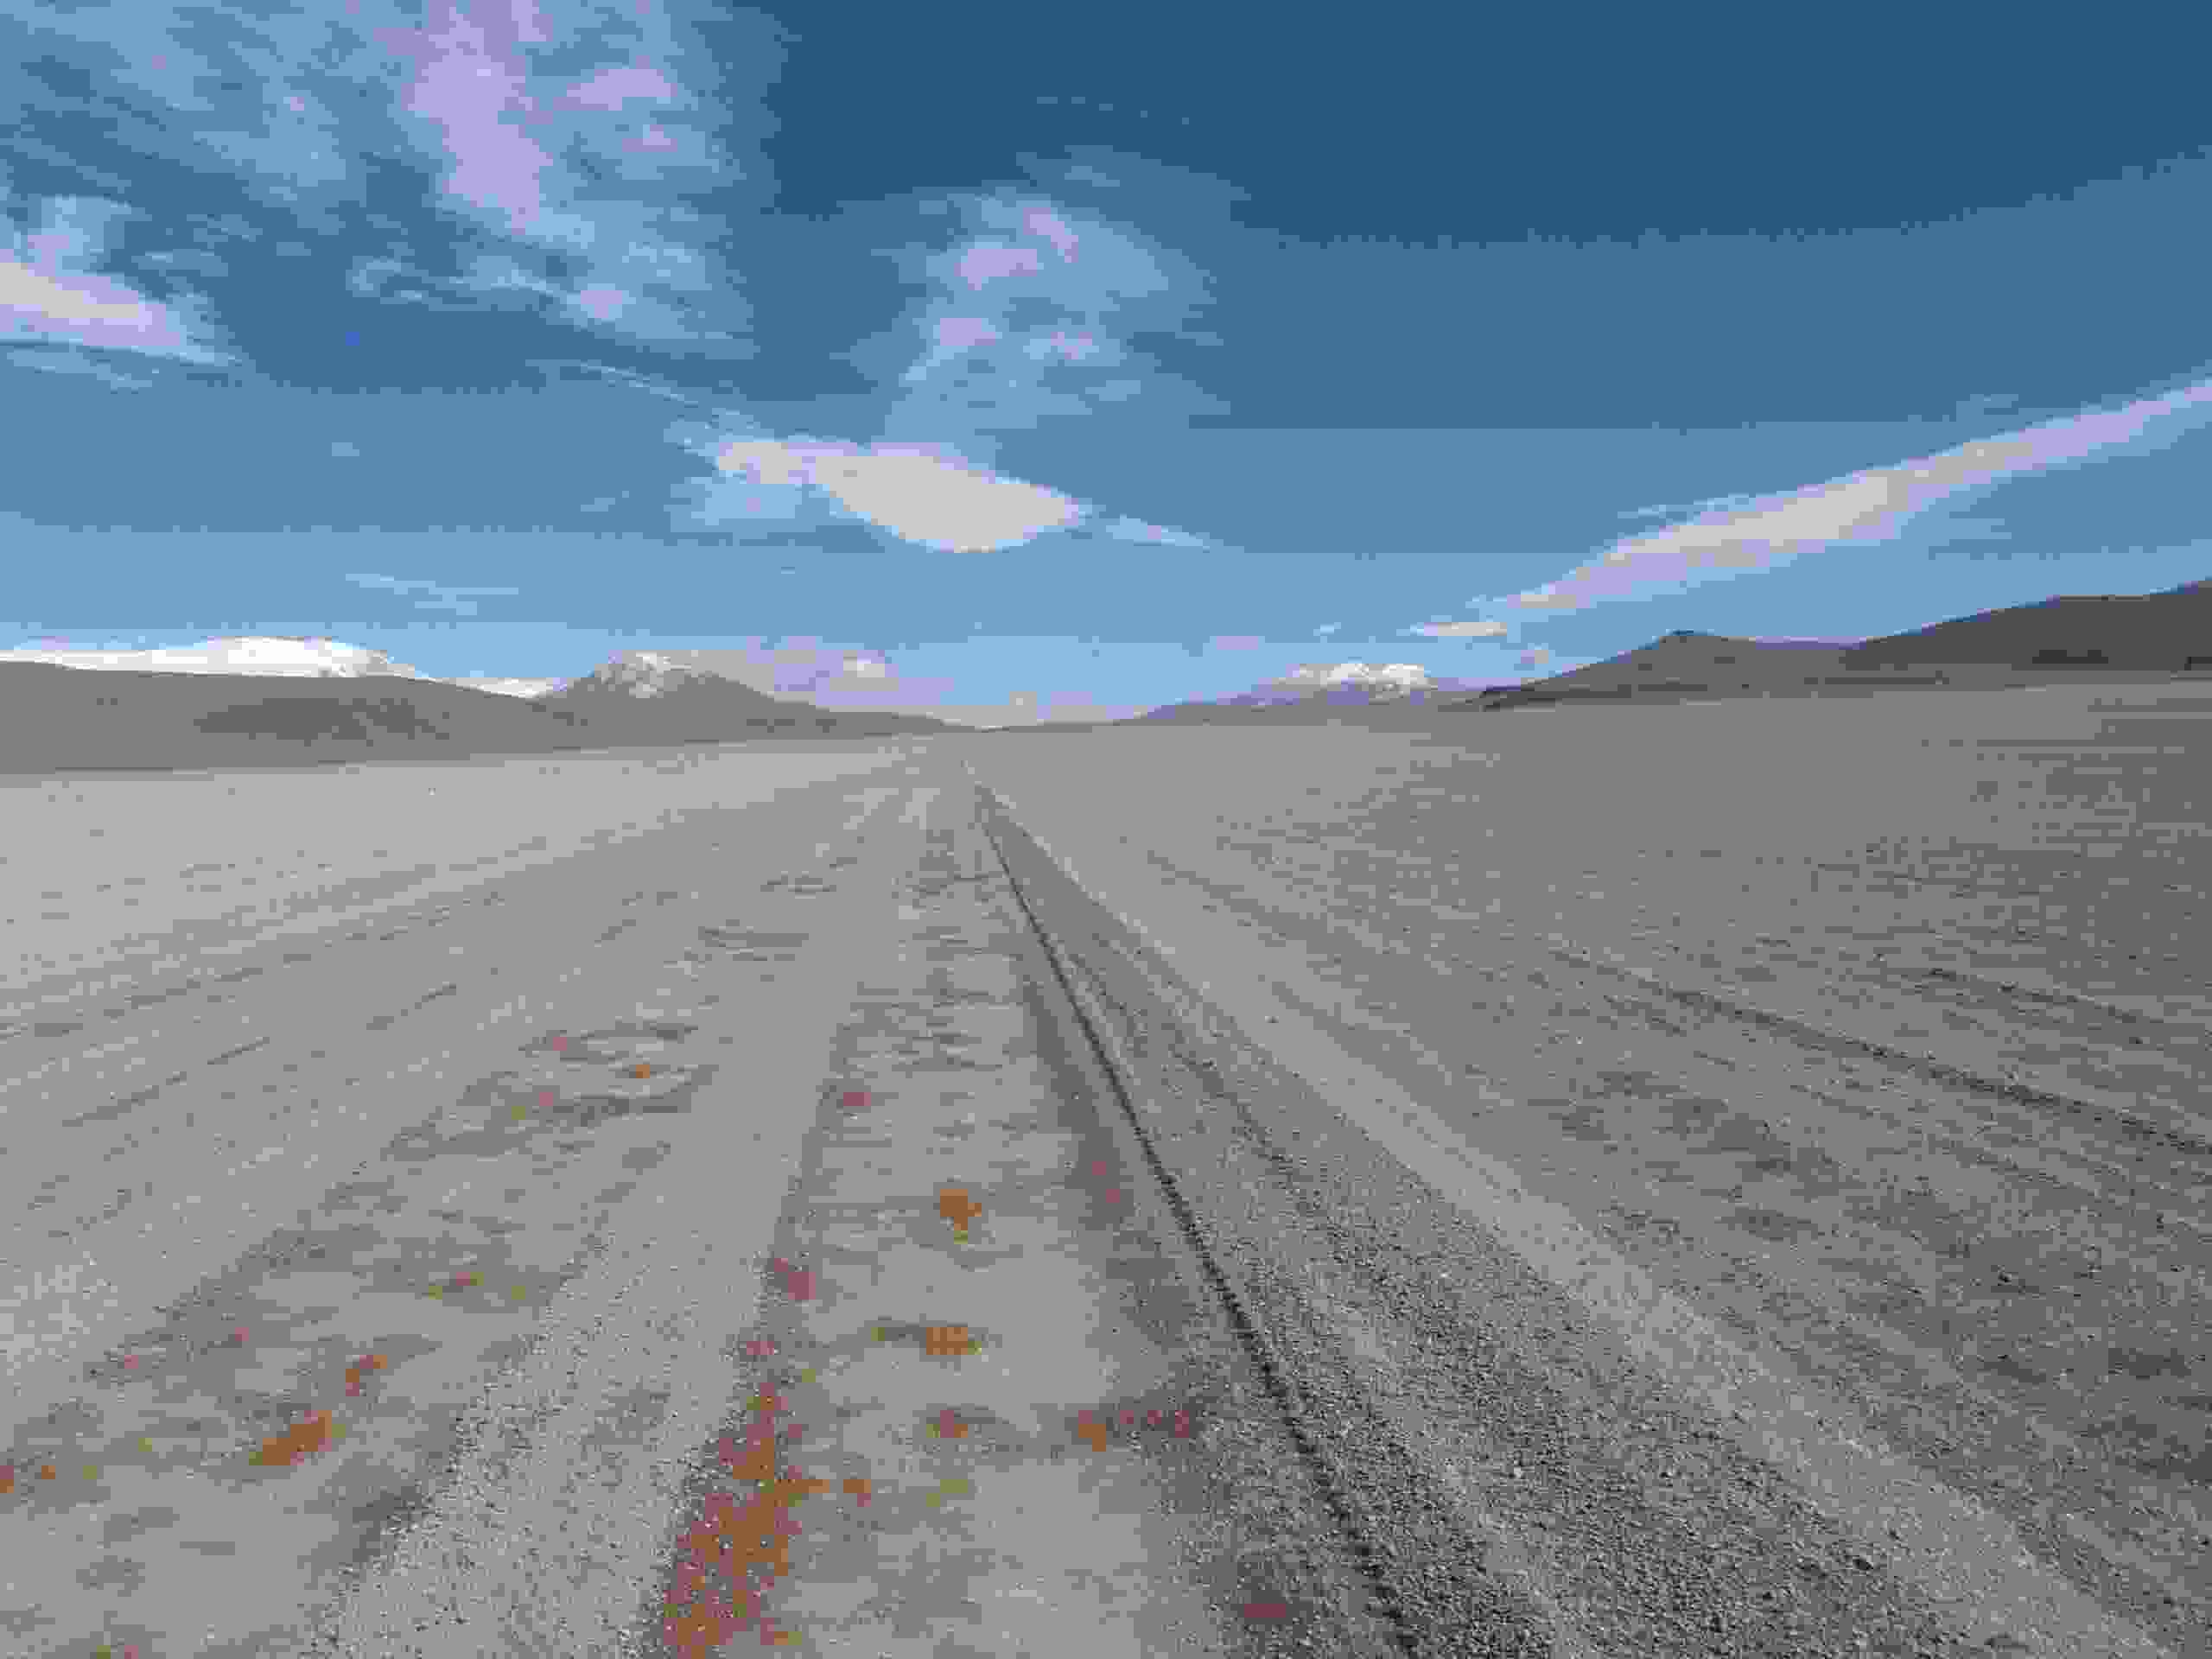
\includegraphics[width=\mywidth]{../wp-content/uploads/2015/04/wpid-wp-1427985056062.jpg} \end{center}

 Pique-nique à l'abri des rochers.
\begin{center} 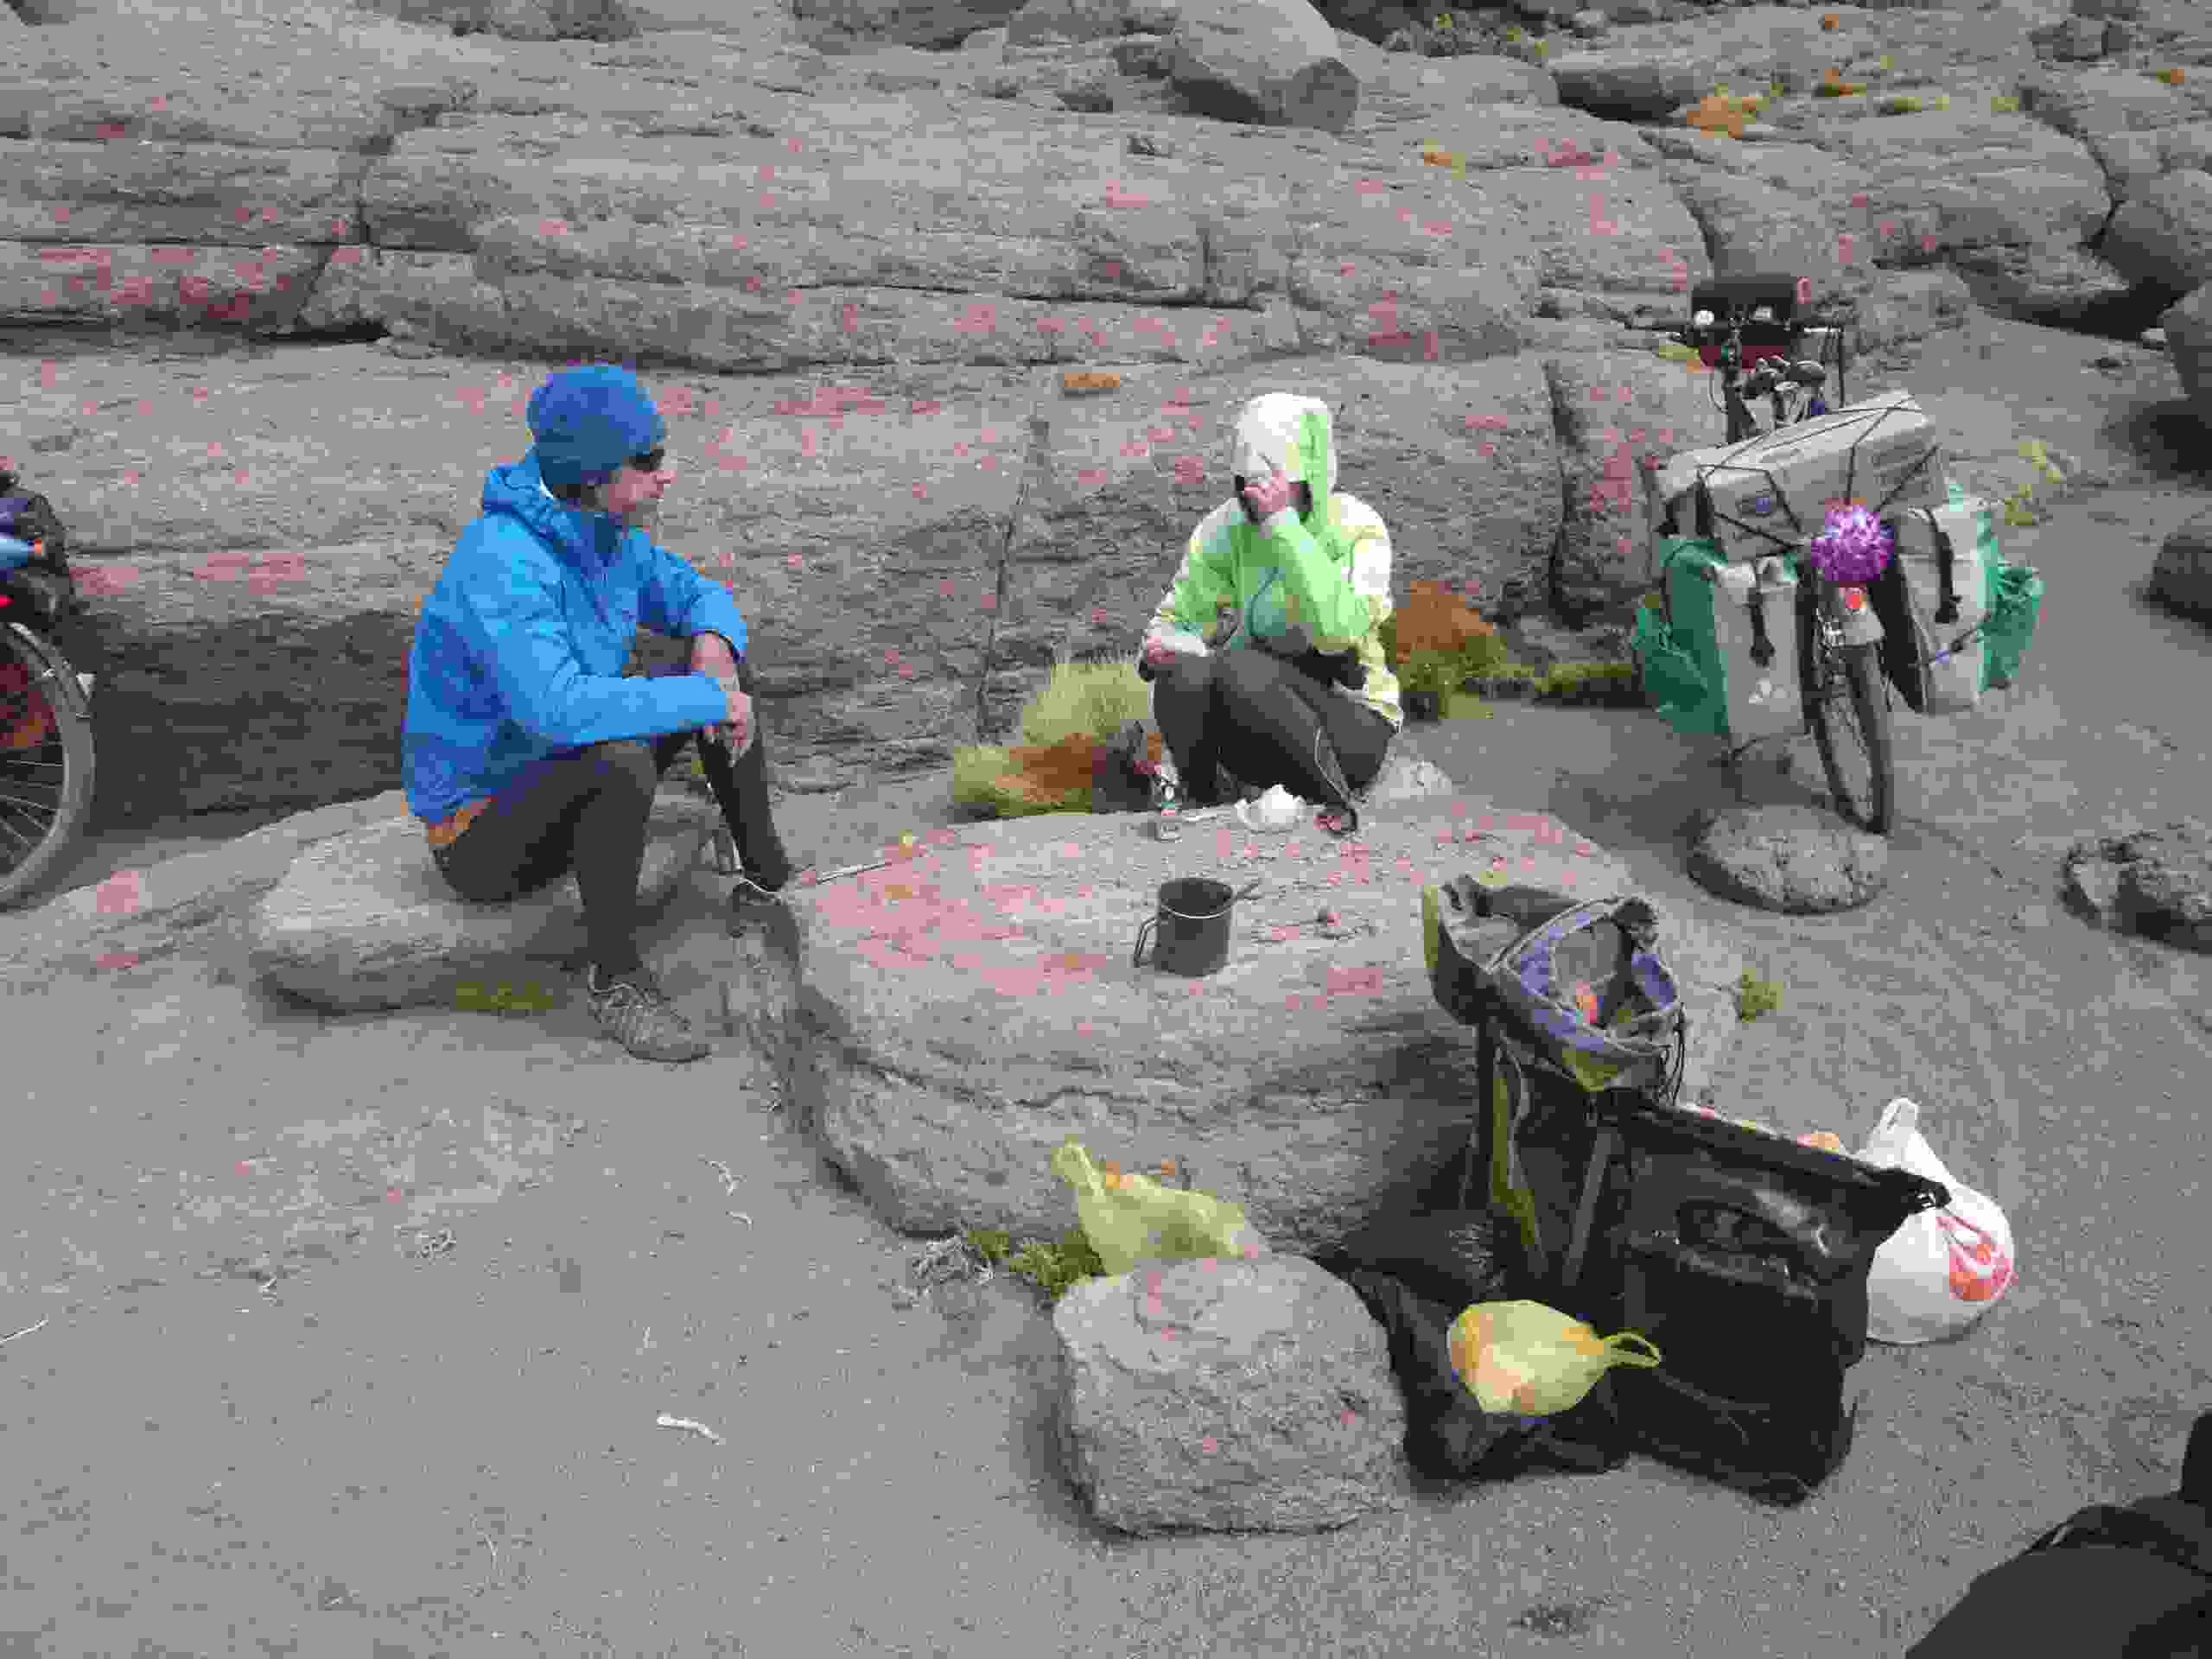
\includegraphics[width=\mywidth]{../wp-content/uploads/2015/04/wpid-wp-1427985094336.jpg} \end{center}

\pagebreak
 Une mousse de la région : au toucher c'est dur comme de la pierre.
\begin{center} 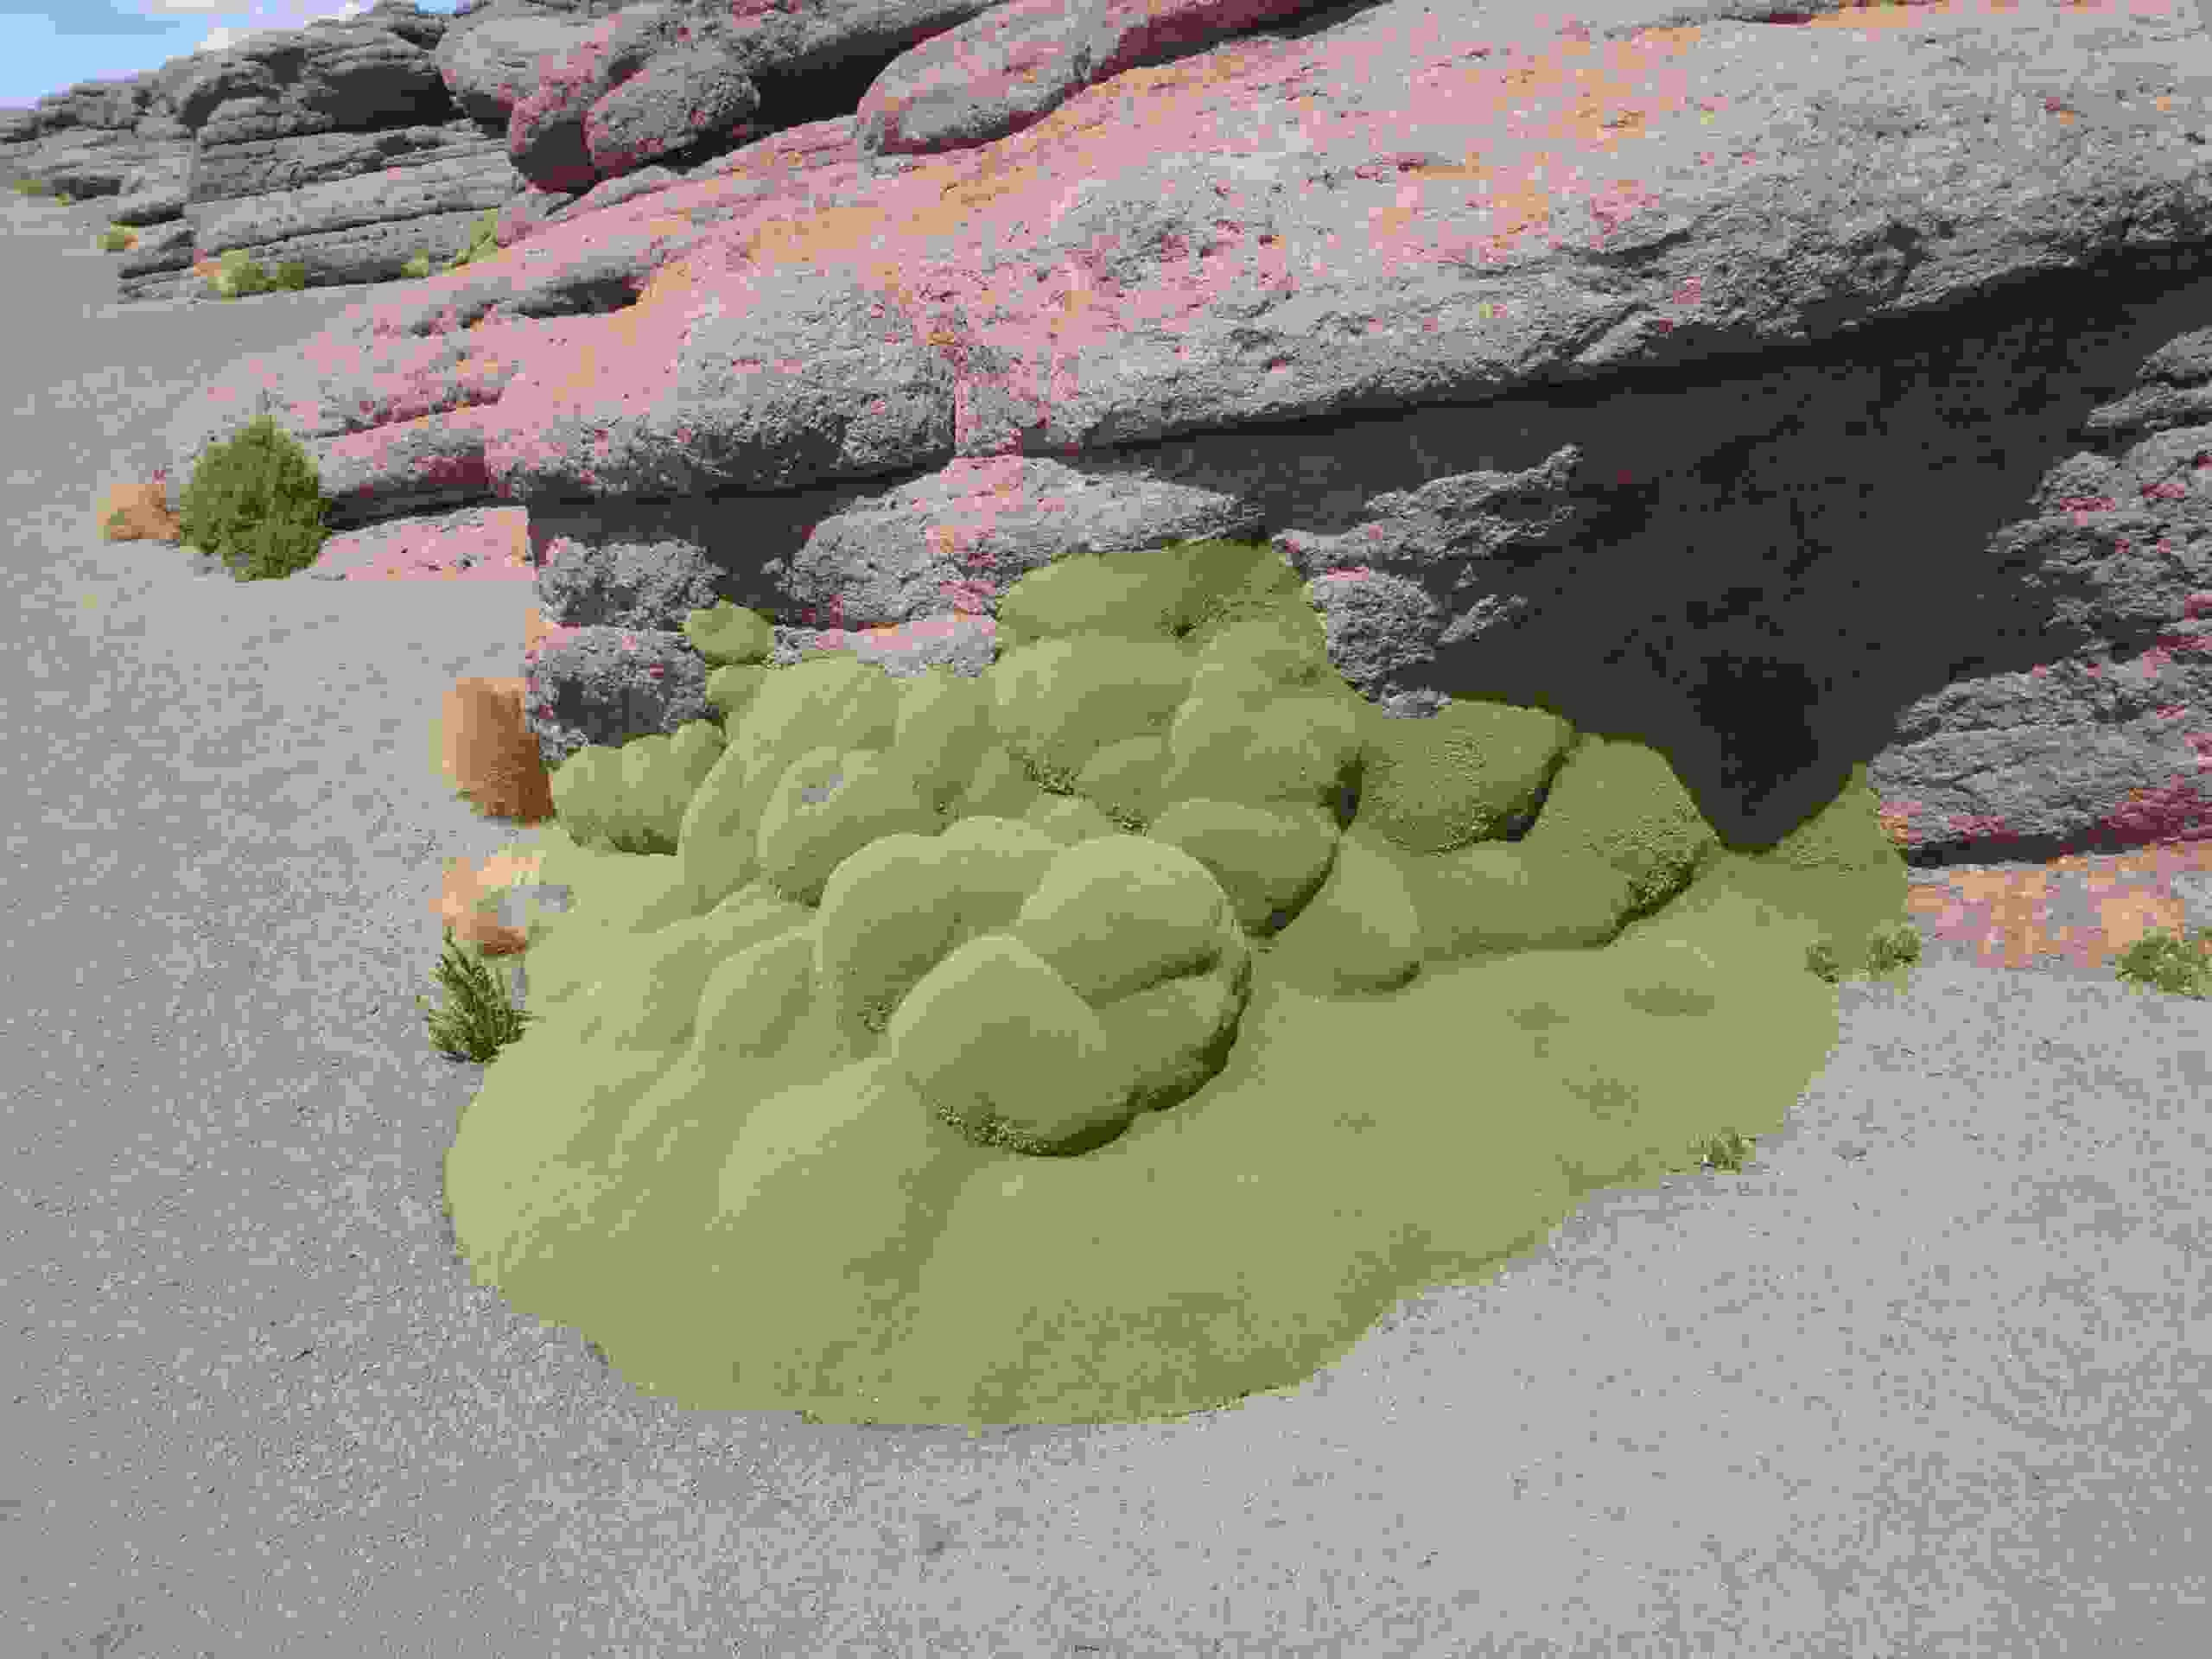
\includegraphics[width=\mywidth]{../wp-content/uploads/2015/04/wpid-wp-1427985074703.jpg} \end{center}

 La fin de journée est horrible avec le vent froid et dans le sable j'arrive épuisé à l'hôtel del Desierto.
\begin{center} 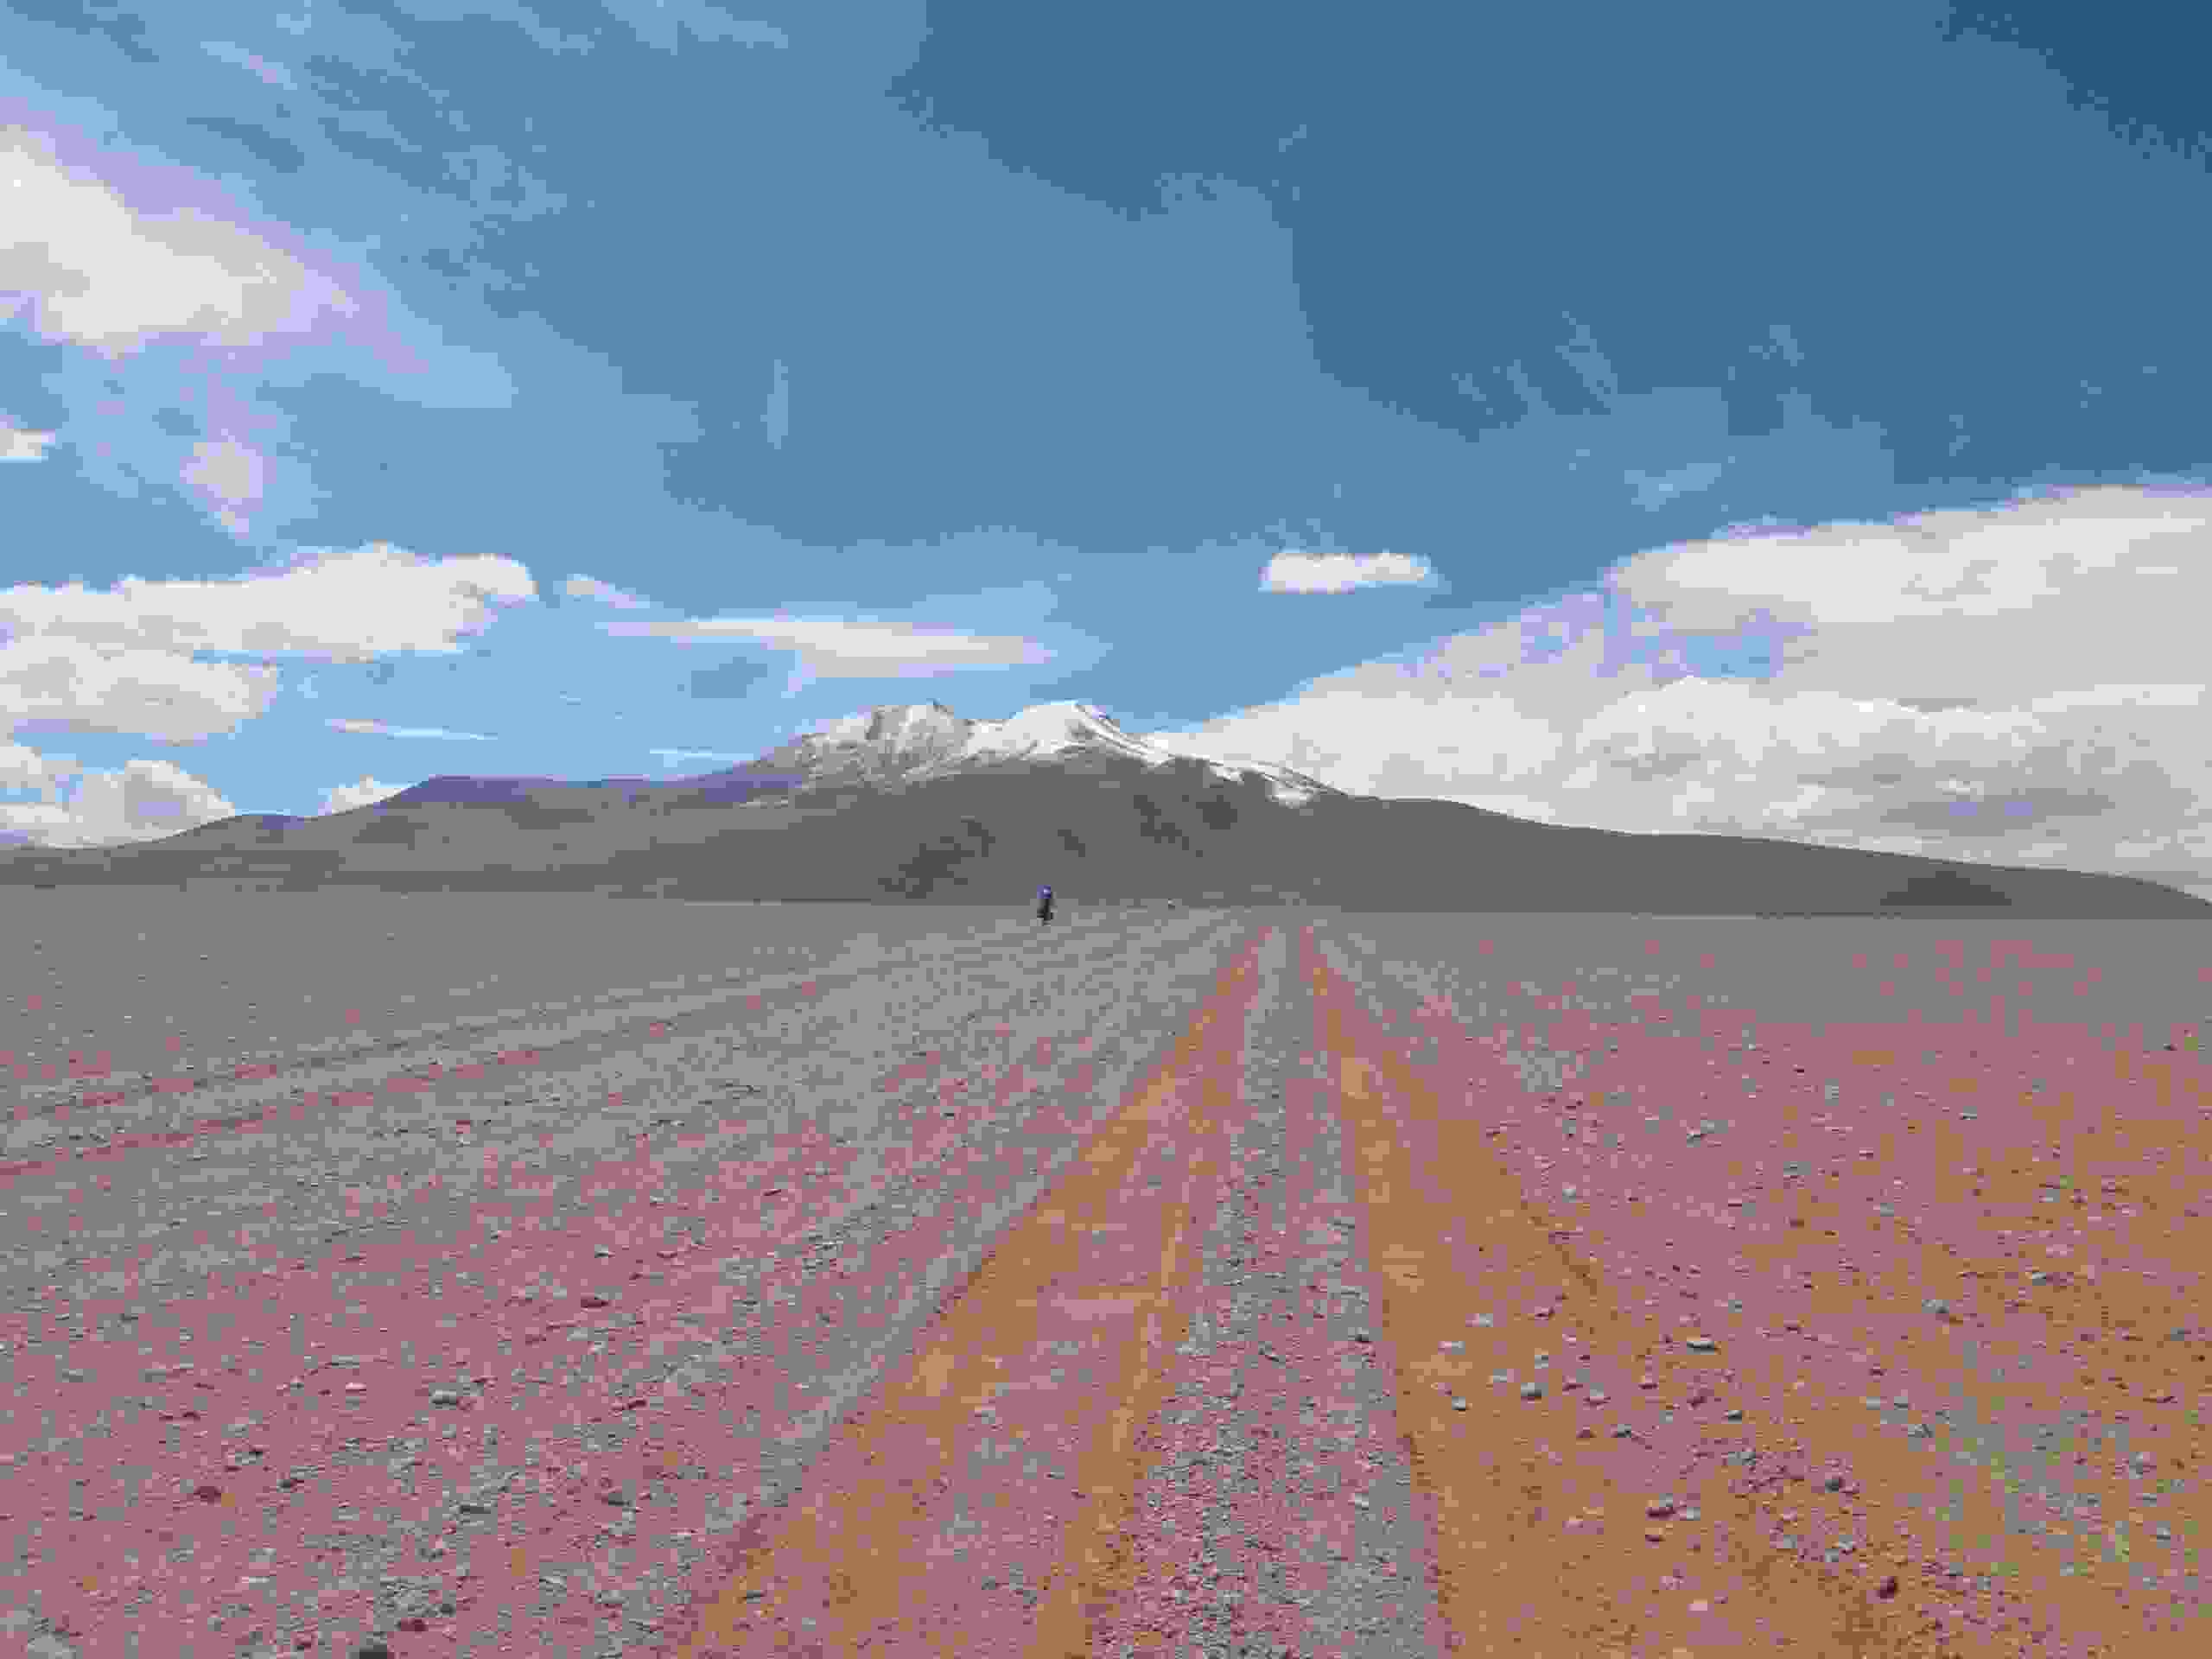
\includegraphics[width=\mywidth]{../wp-content/uploads/2015/04/wpid-wp-1427985137543.jpg} \end{center}

  On nous annonce un prix exorbitant de 150 dollars pour la nuit, heureusement on arrive à obtenir le tarif bolivien, environ un tiers du prix. J'avais bien besoin d'un vrai lit pour récupérer.
\begin{center} 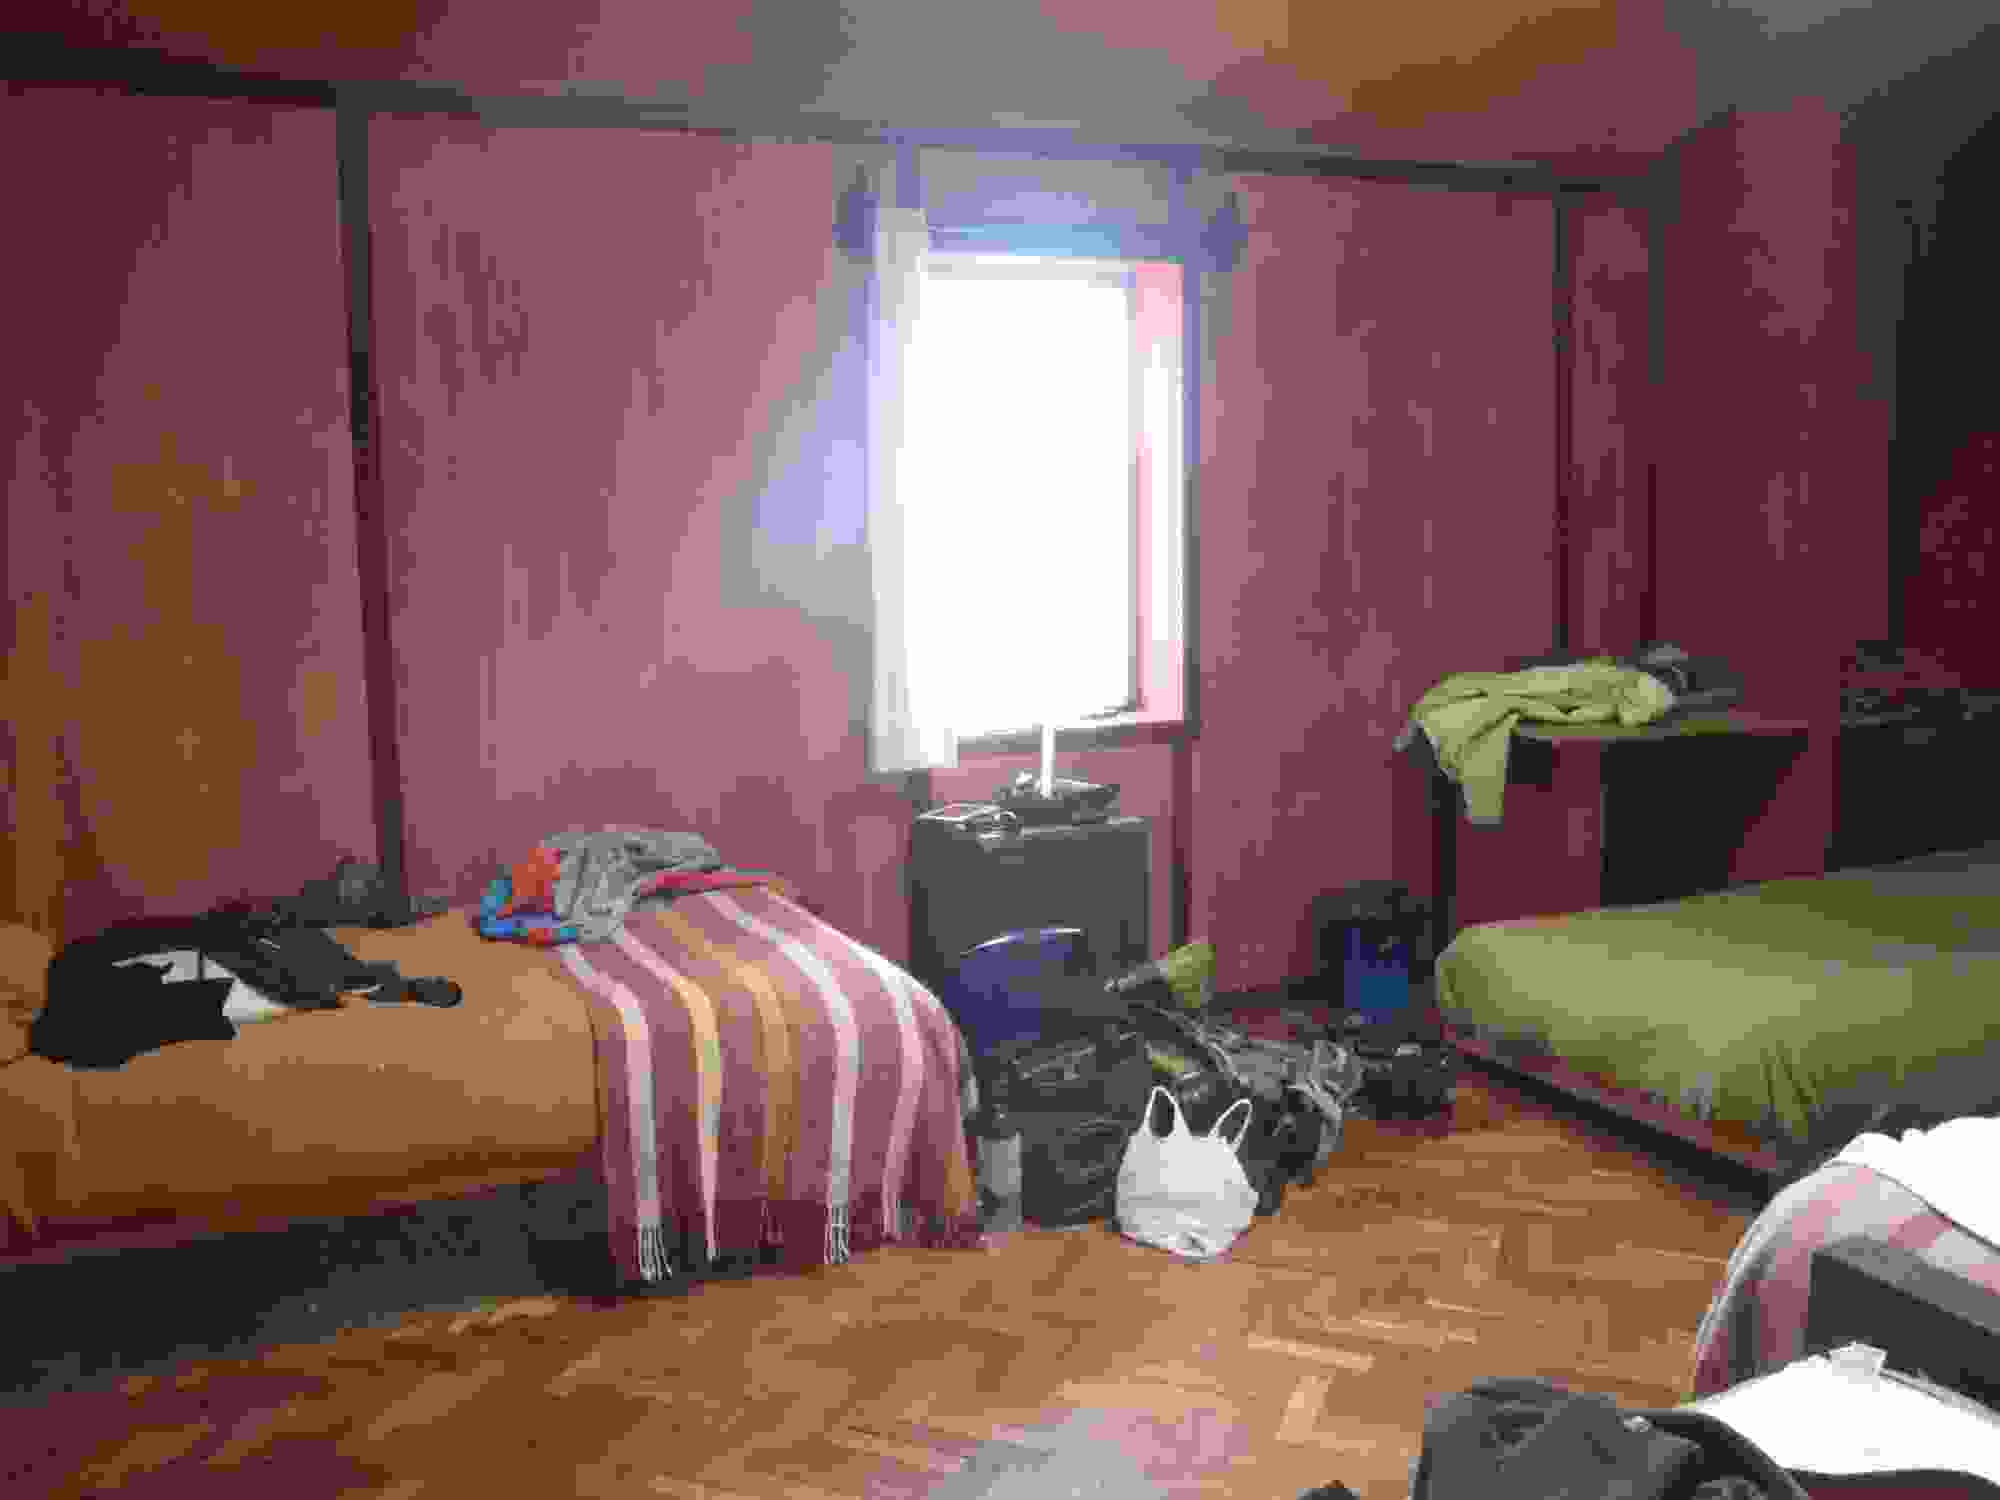
\includegraphics[width=\mywidth]{../wp-content/uploads/2015/04/wpid-wp-1427989235491.jpg} \end{center}

 \subsection*{7\ieme\ jour} 

 Première partie encore difficile et dans le vent mais grand ciel bleu : bon pour le moral.
\begin{center} 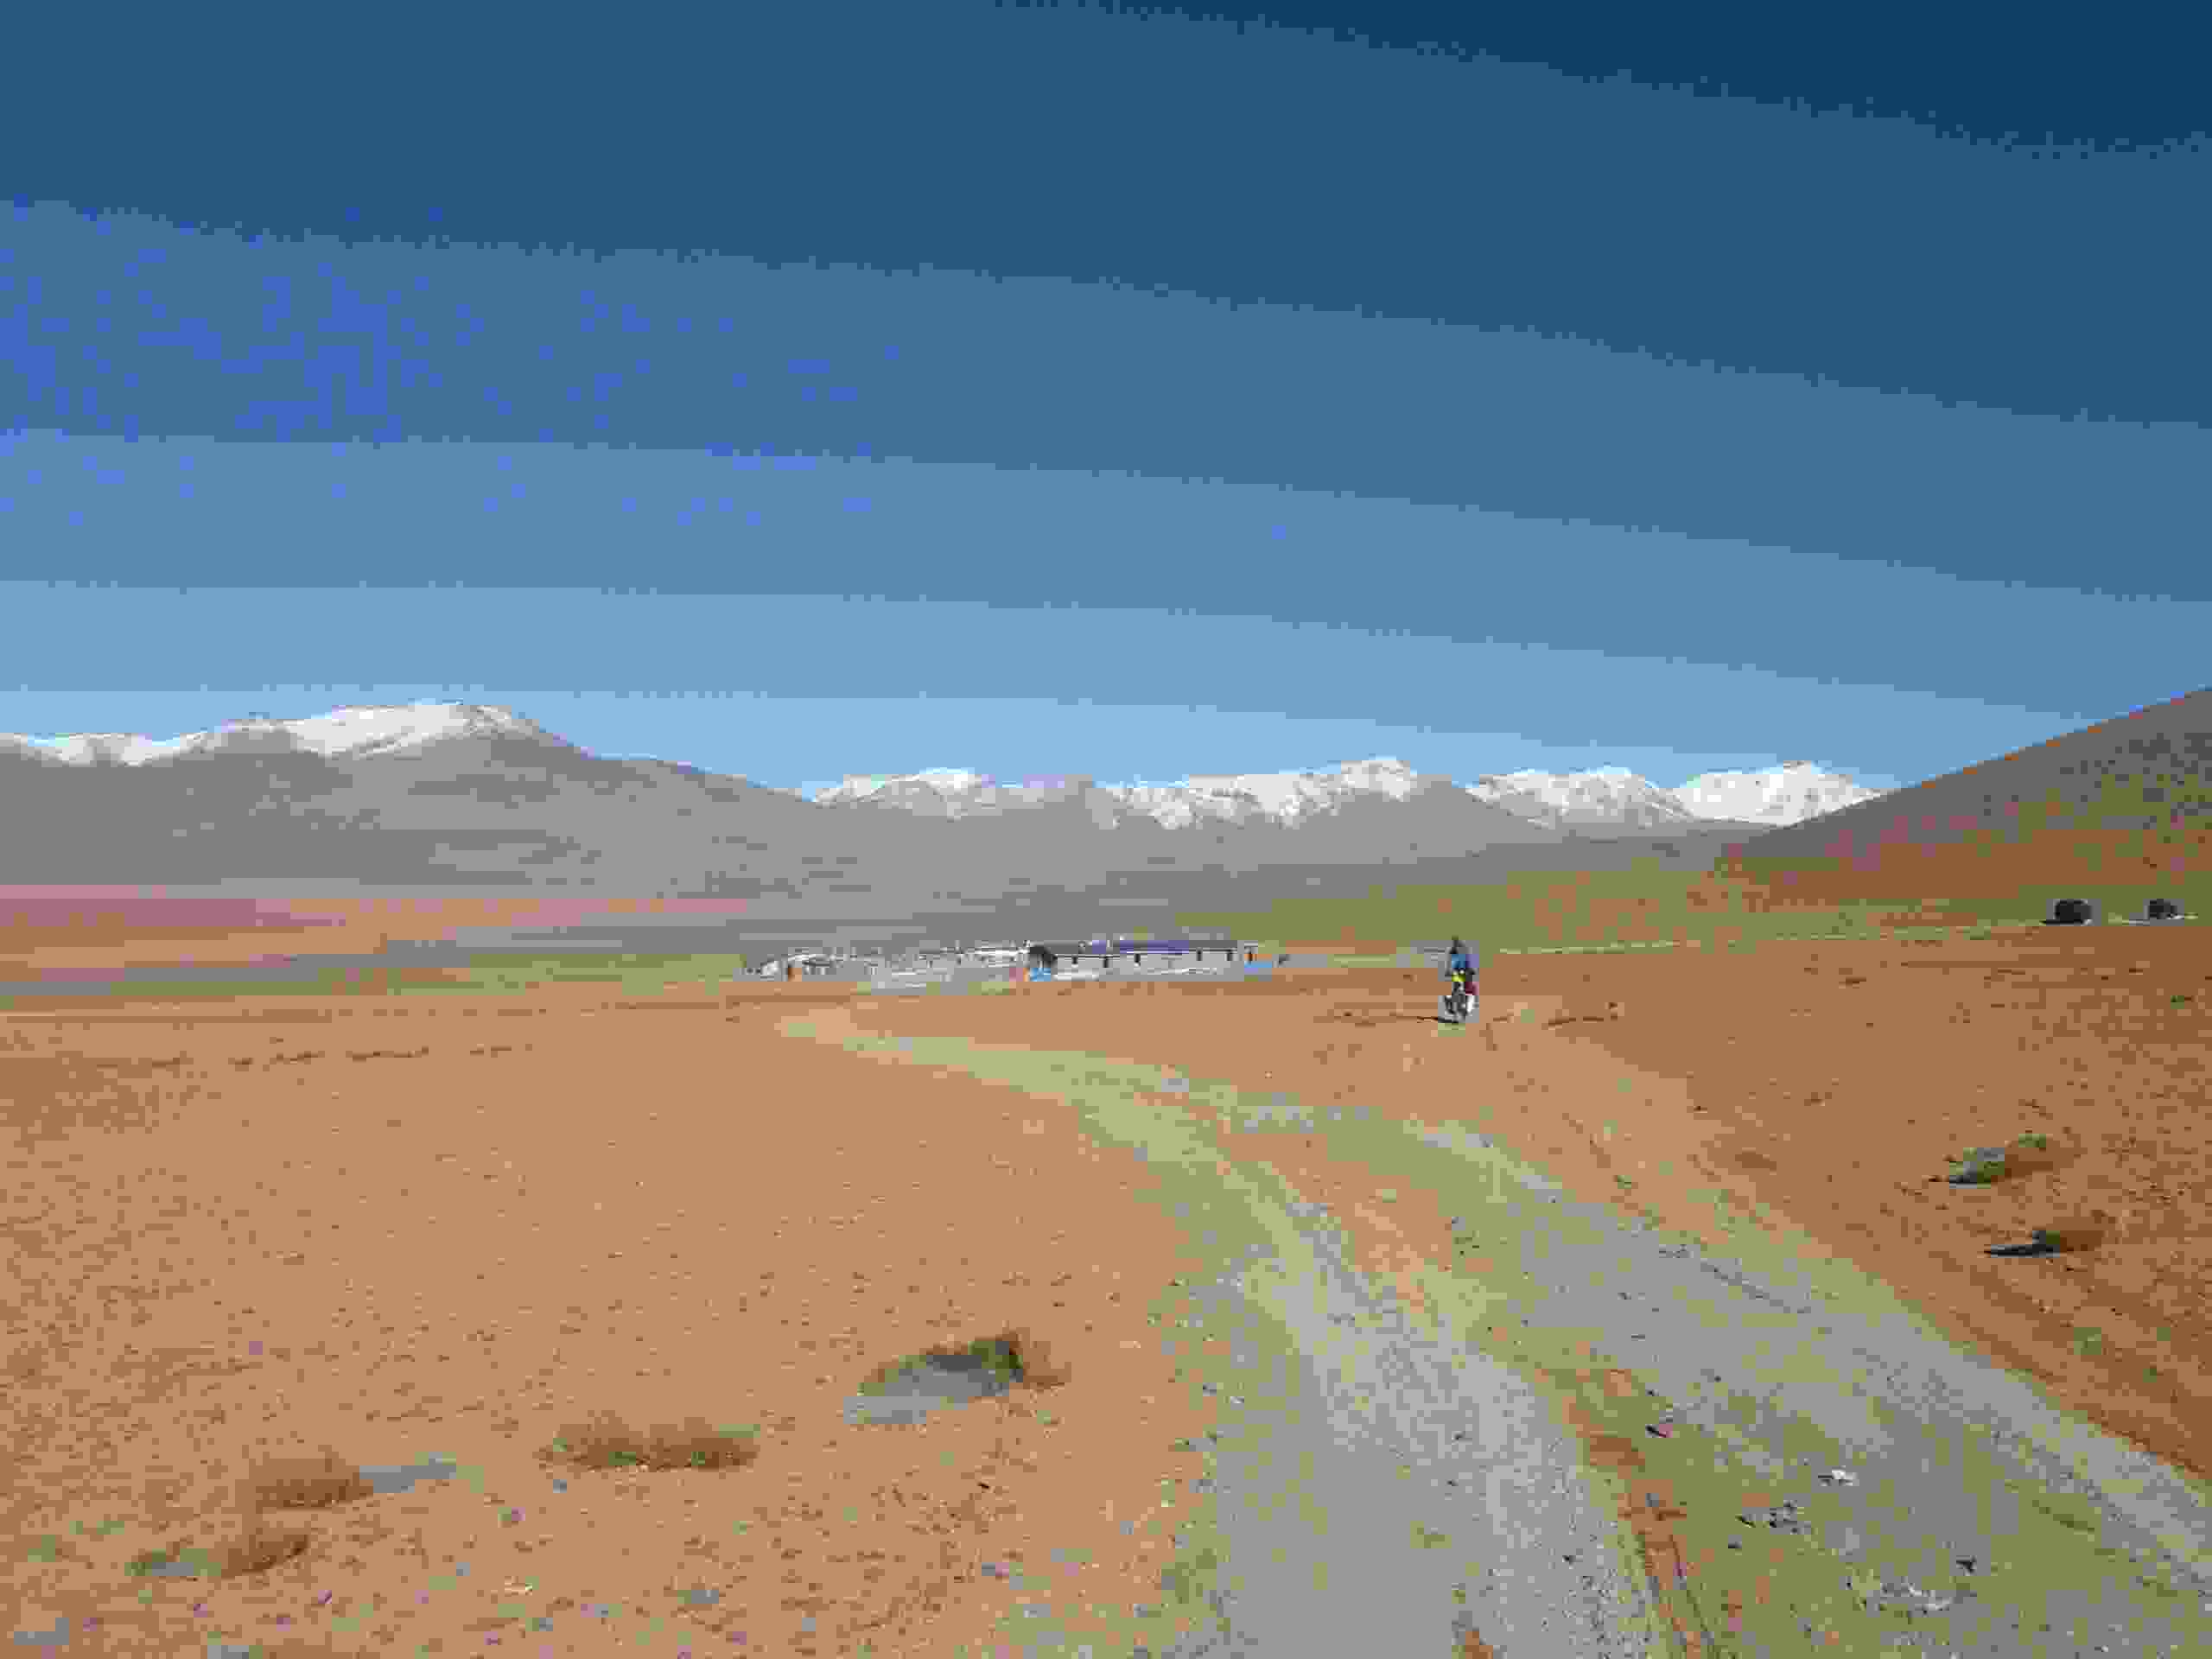
\includegraphics[width=\mywidth]{../wp-content/uploads/2015/04/wpid-wp-1427985164097.jpg} \end{center}
\begin{center} 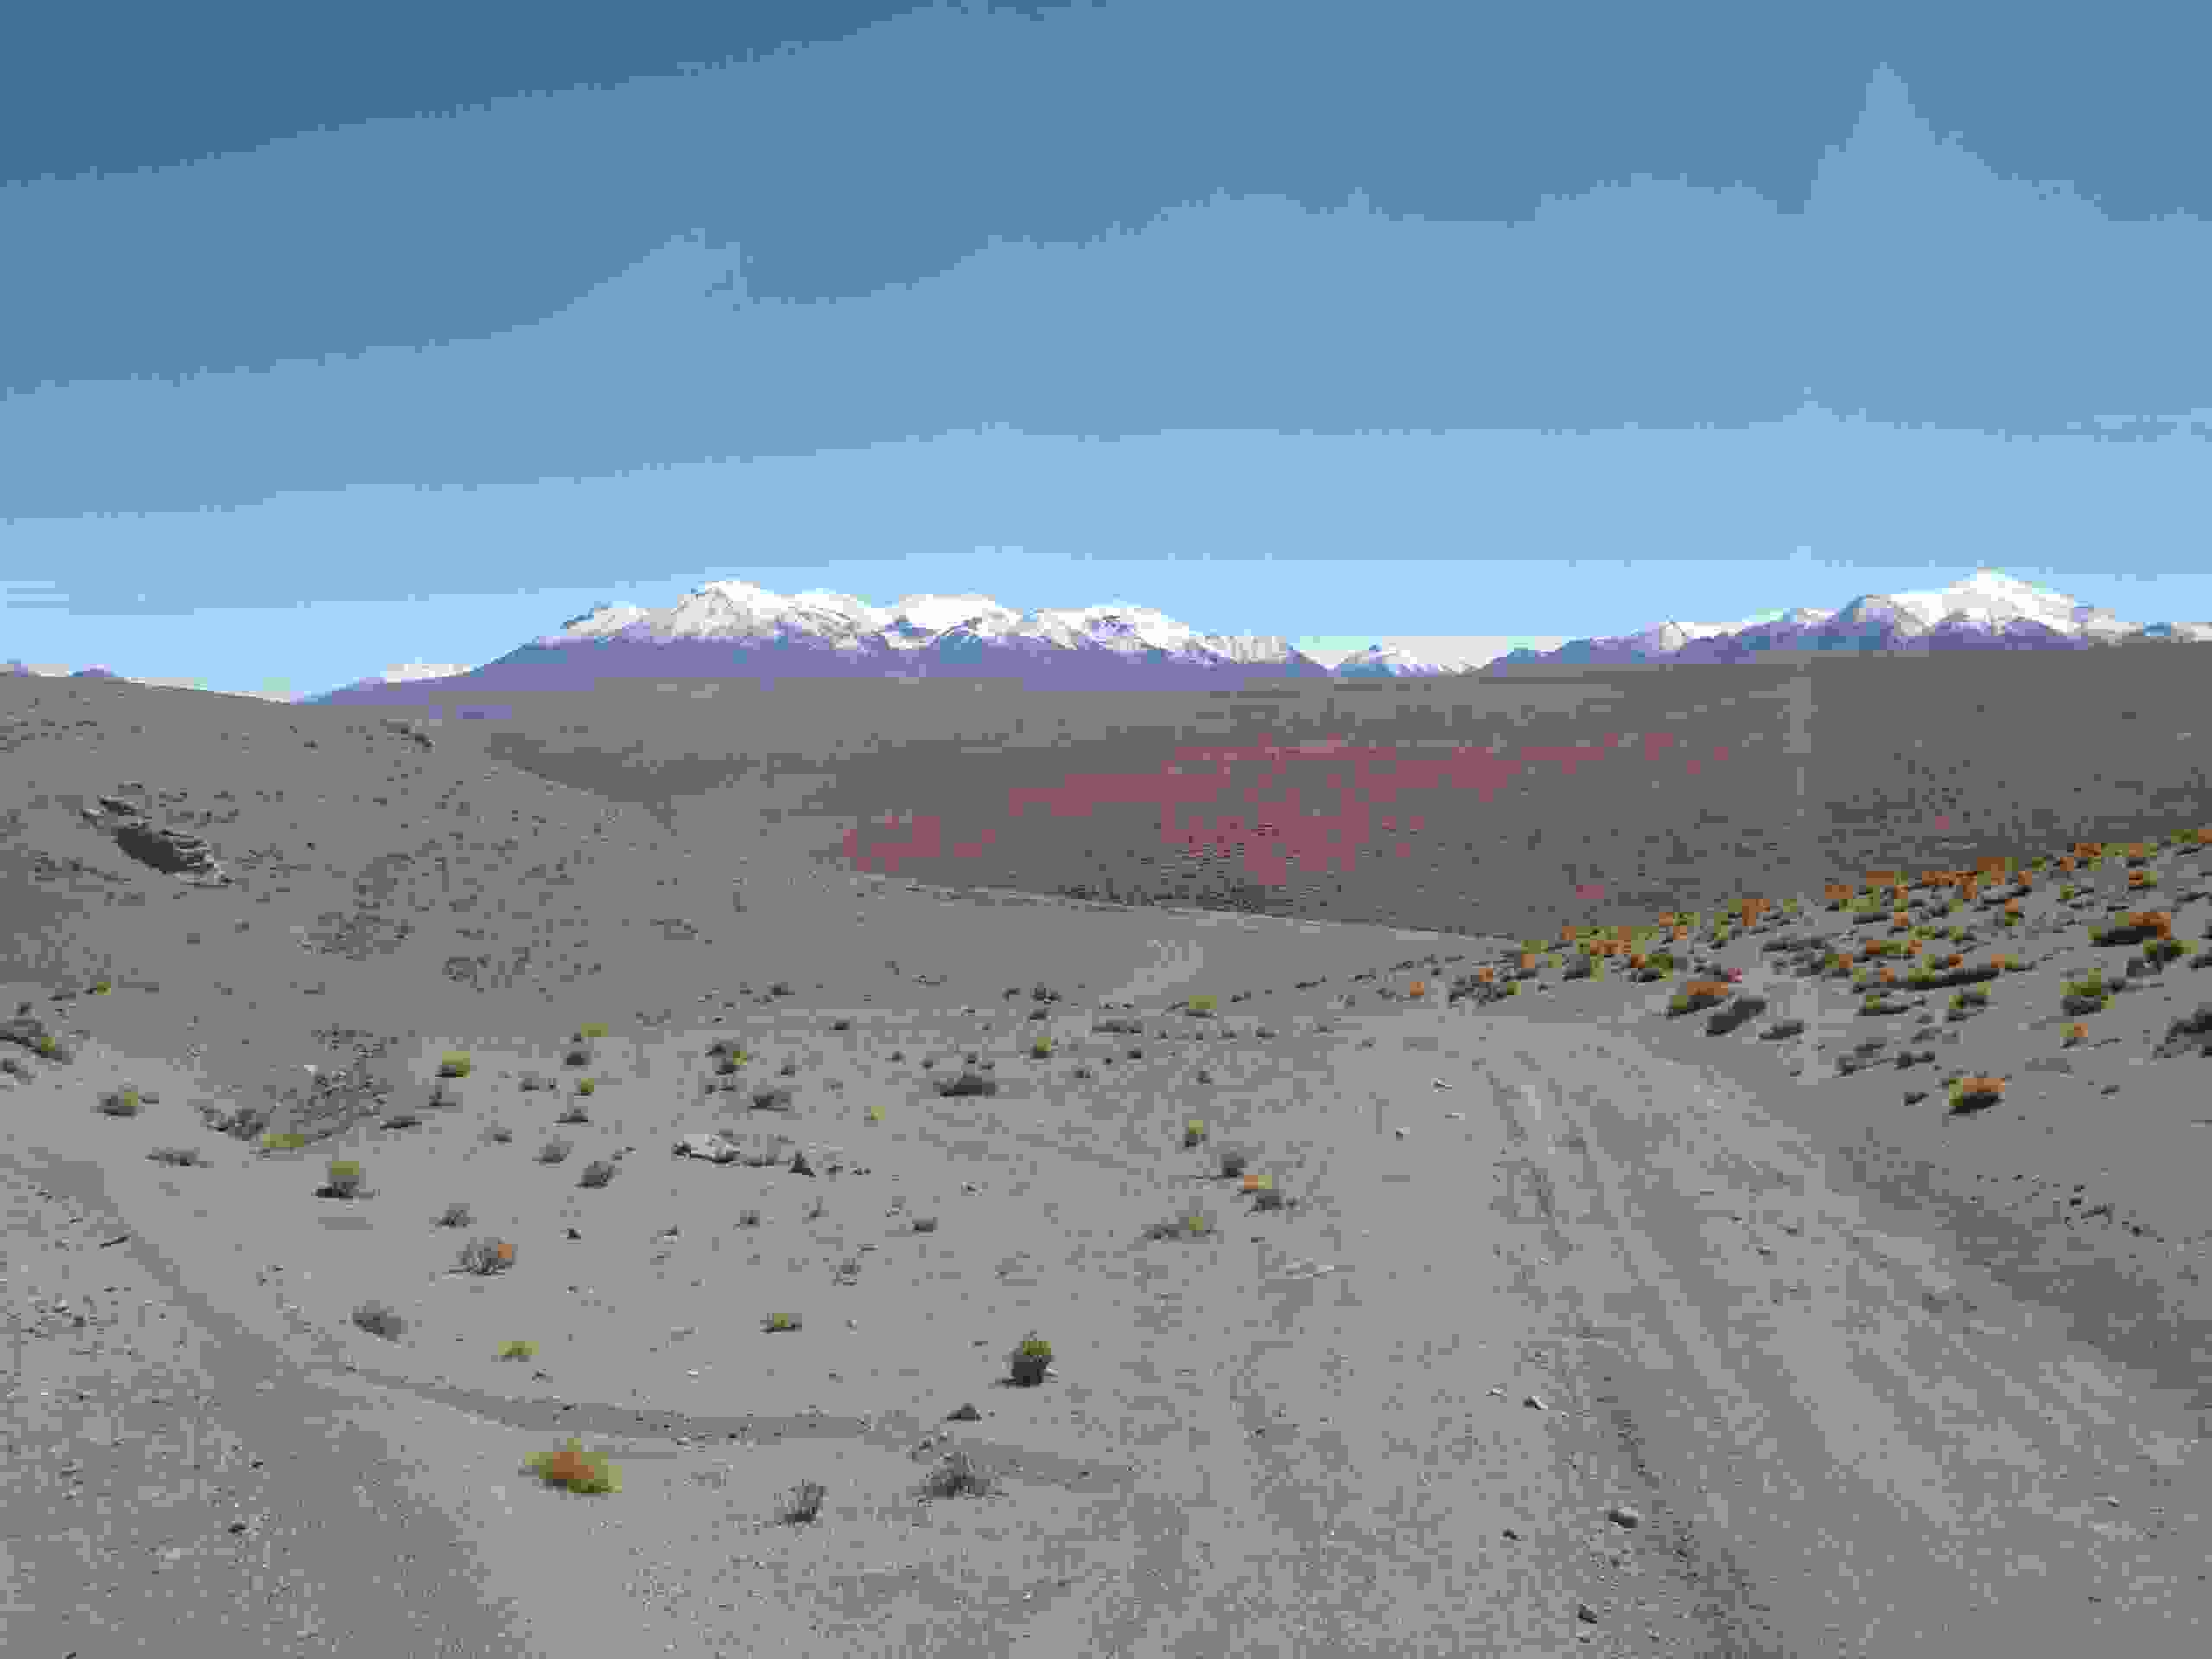
\includegraphics[width=\mywidth]{../wp-content/uploads/2015/04/wpid-wp-1427985190000.jpg} \end{center}

  Puis c'est la descente et on arrive sur une succession de lacs magnifiques.
\begin{center} 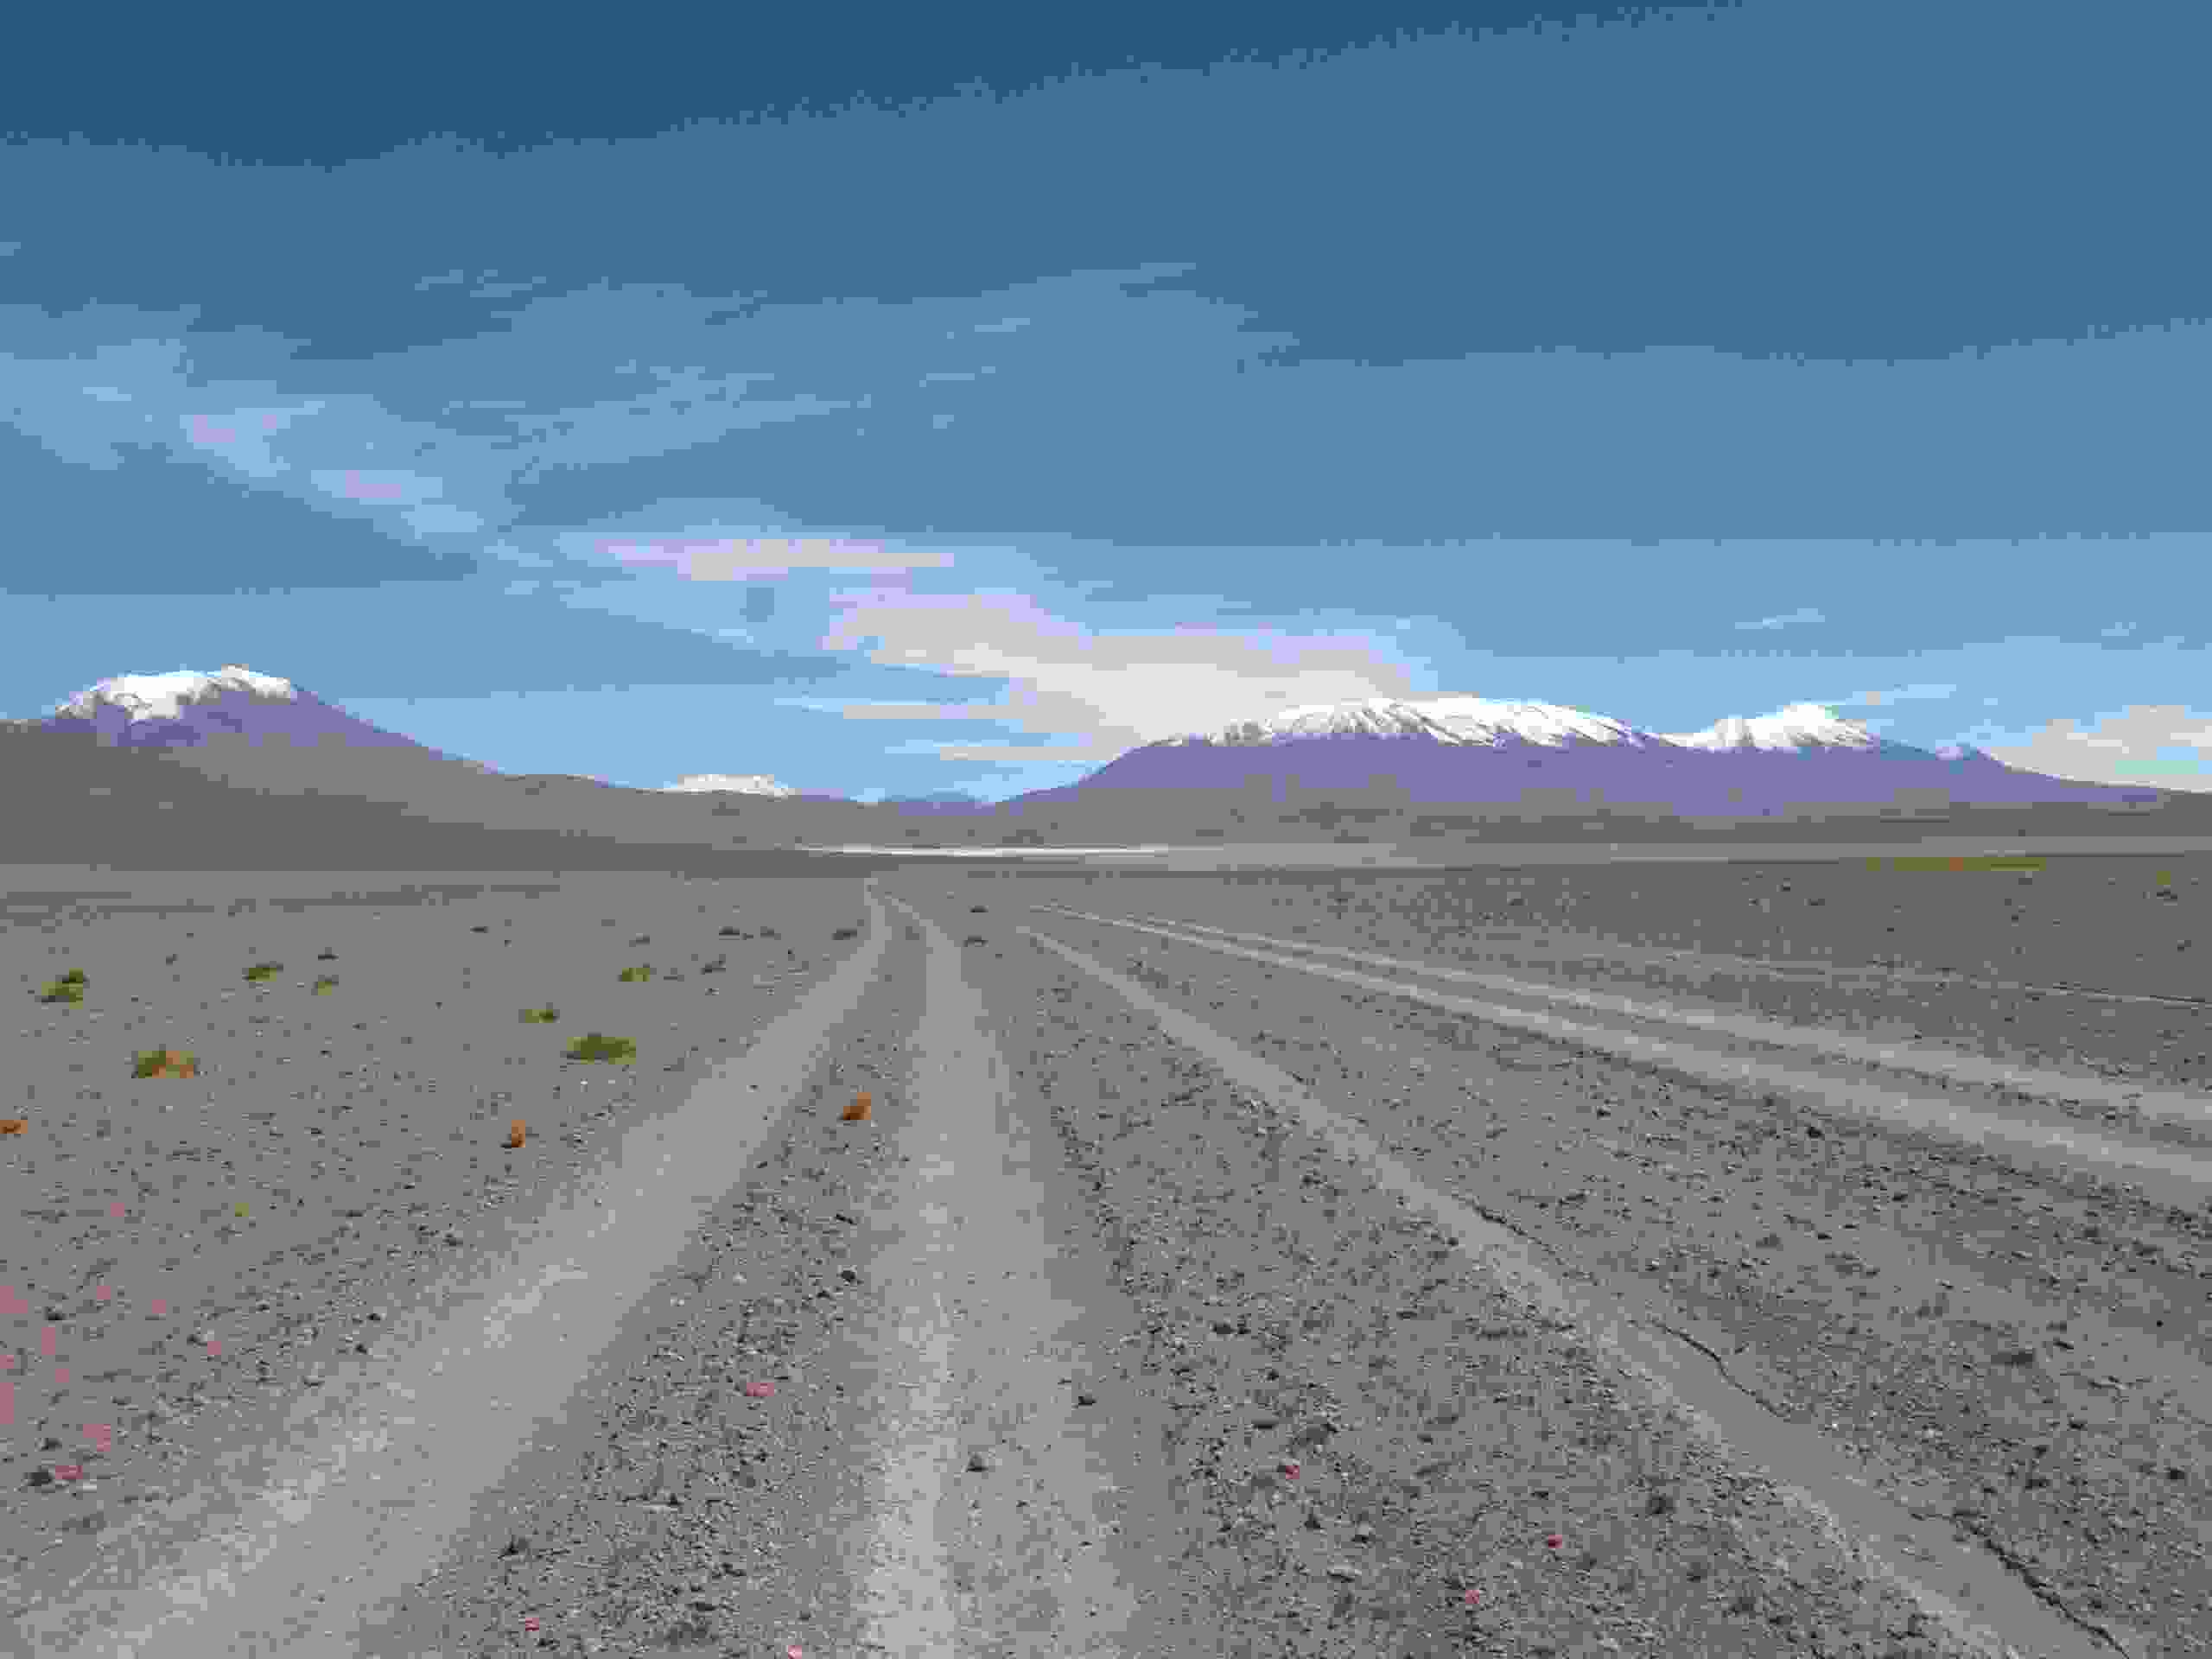
\includegraphics[width=\mywidth]{../wp-content/uploads/2015/04/wpid-wp-1427985235958.jpg} \end{center}
\begin{center} 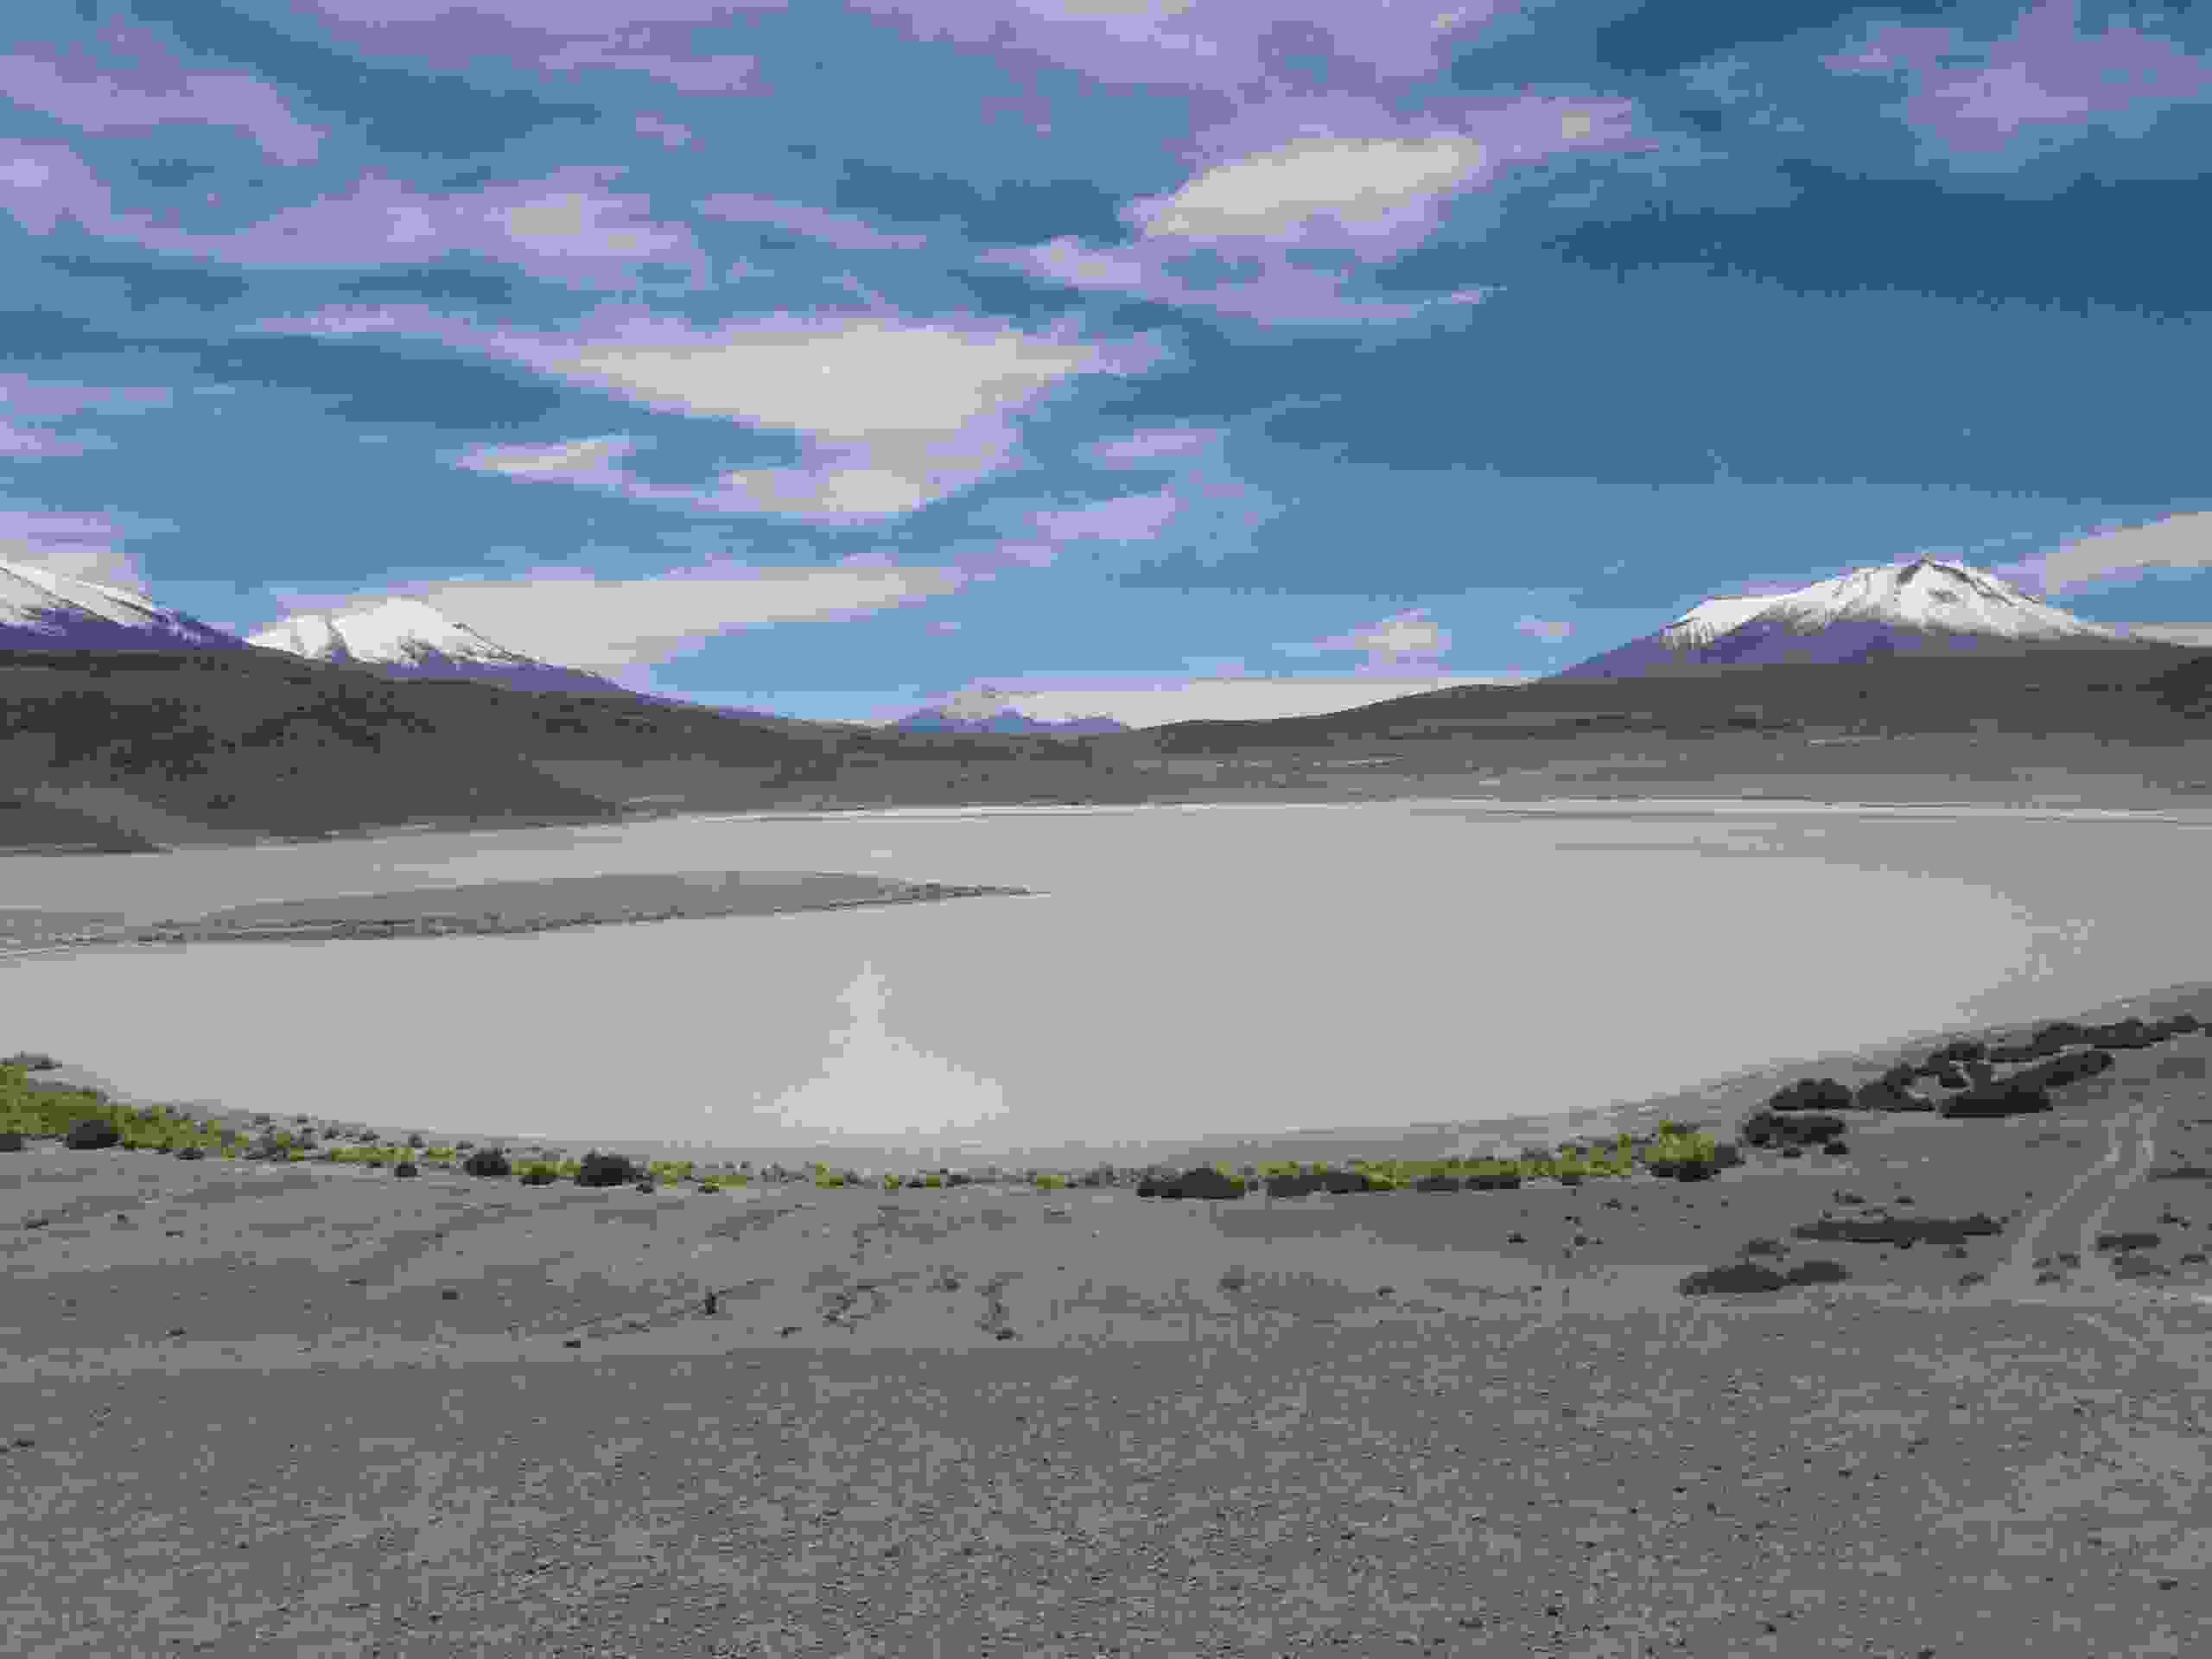
\includegraphics[width=\mywidth]{../wp-content/uploads/2015/04/wpid-wp-1427985282277.jpg} \end{center}
\begin{center} 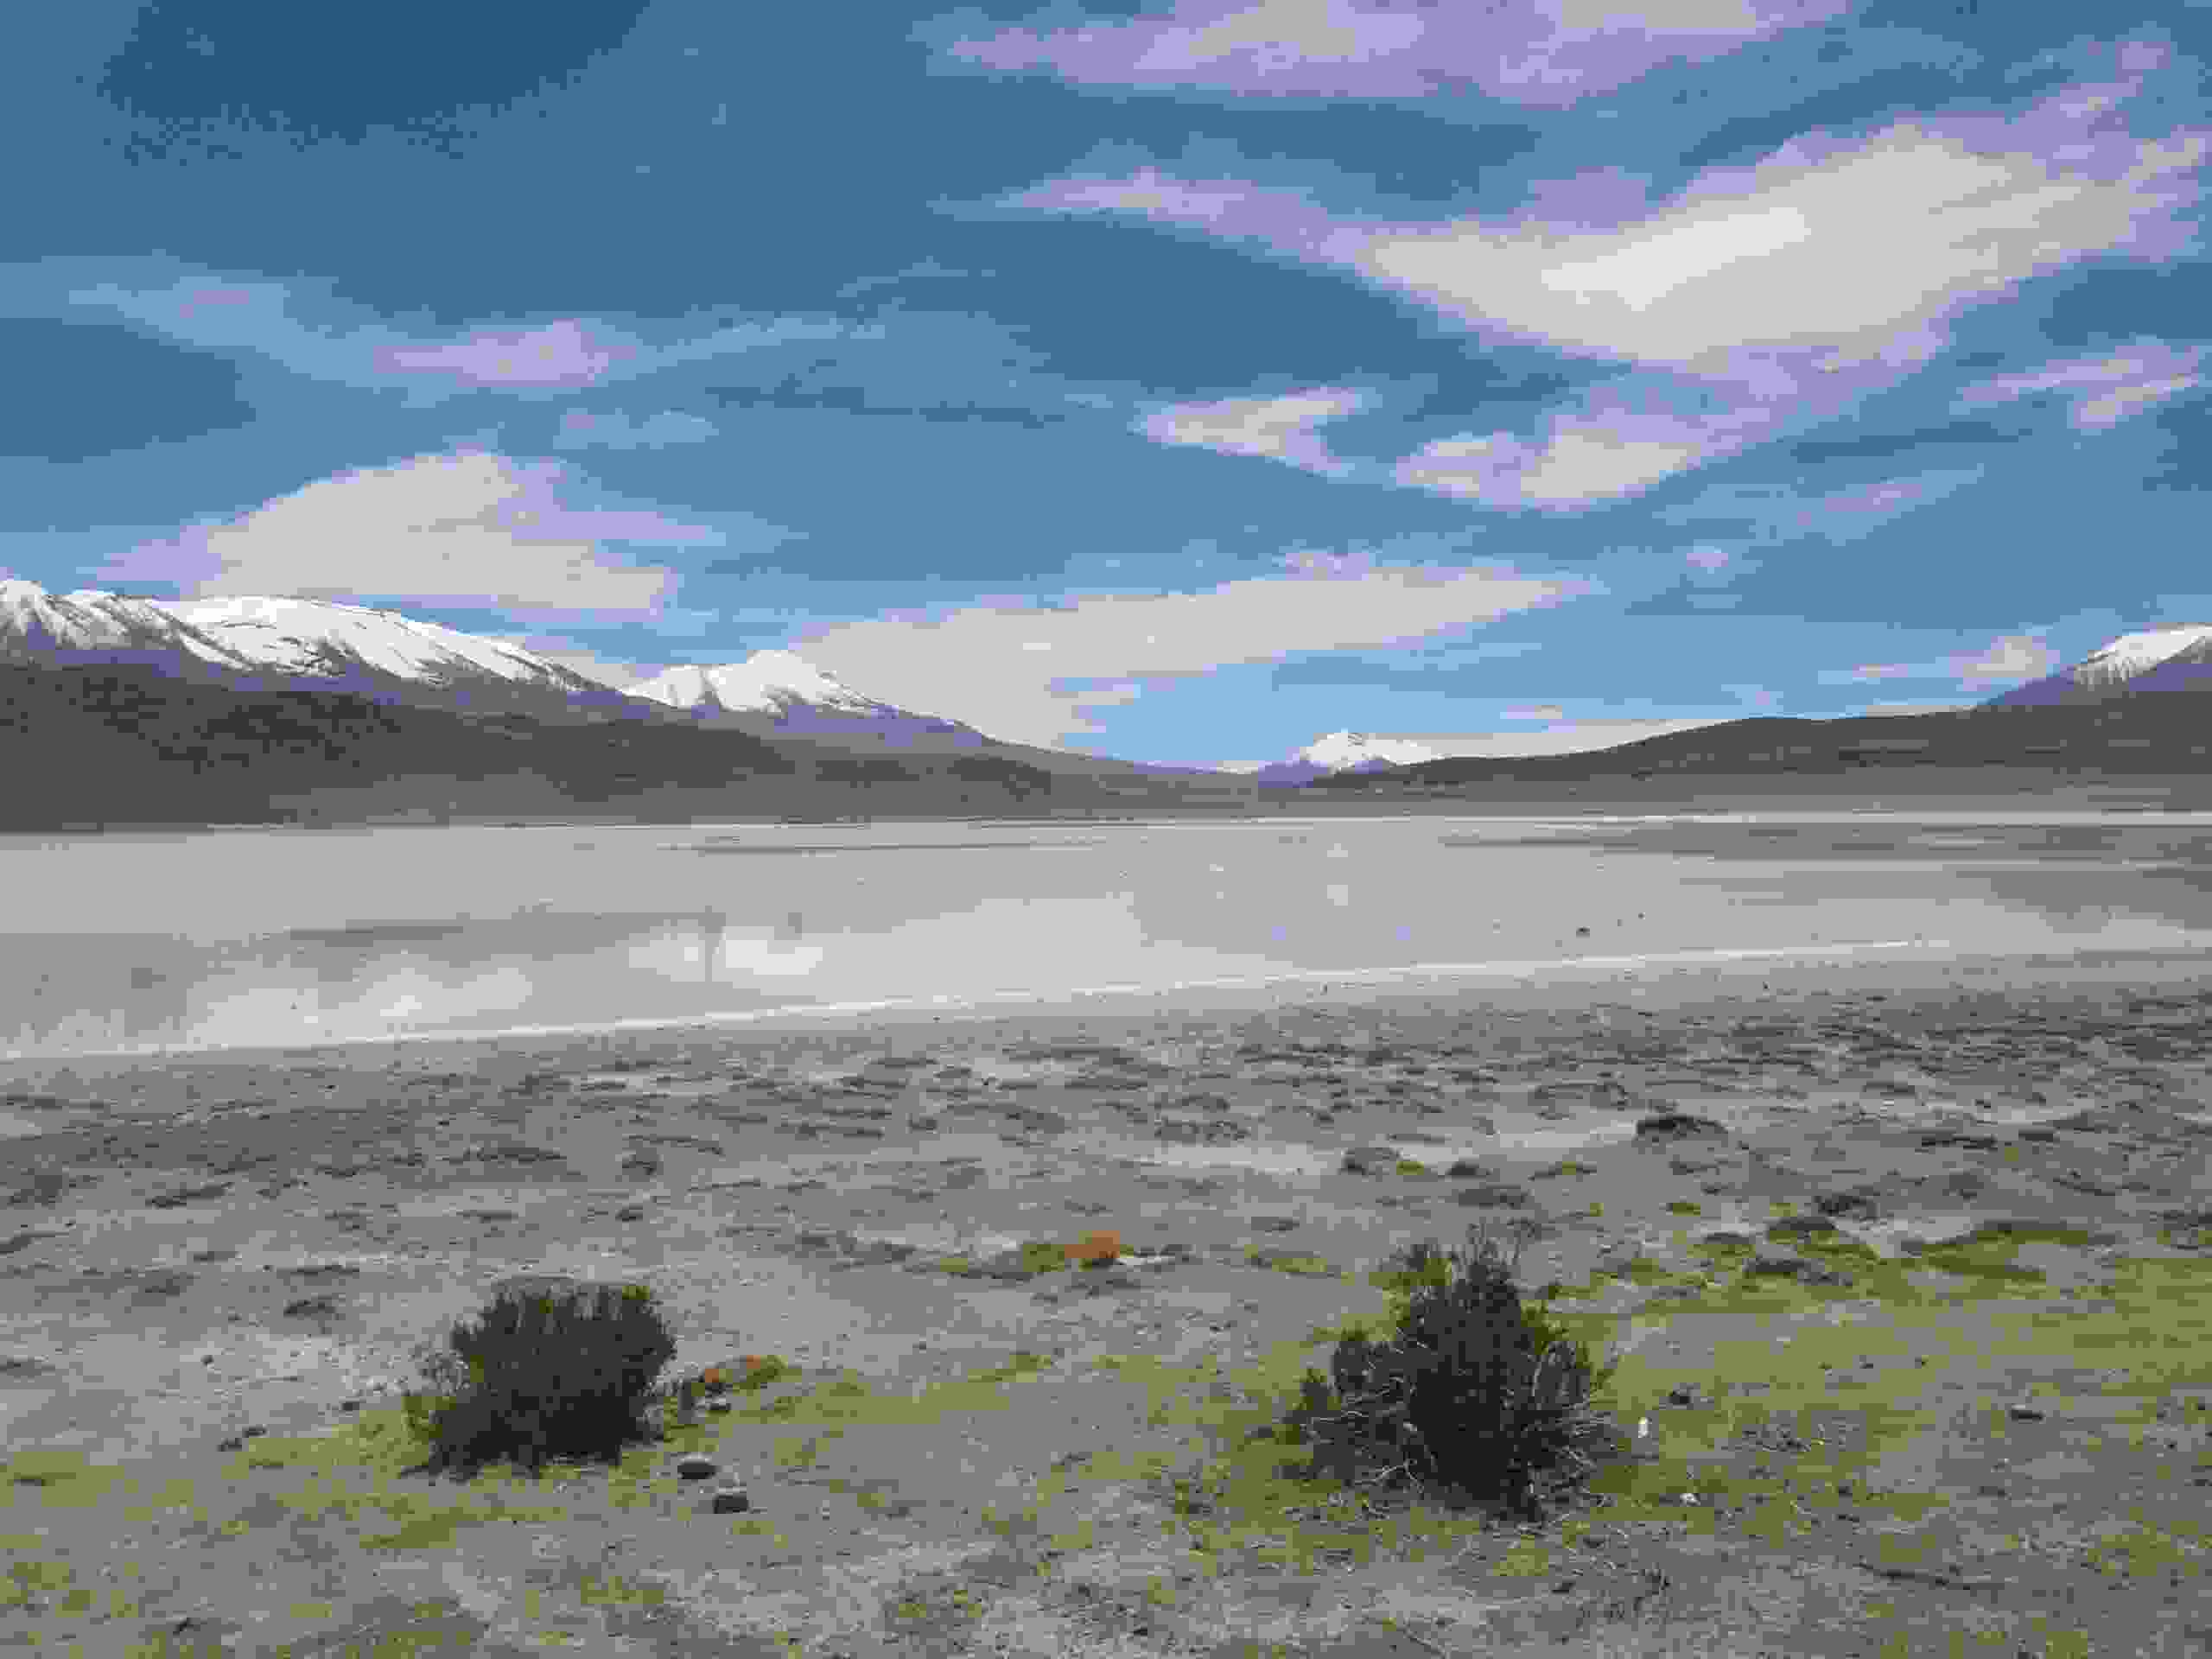
\includegraphics[width=\mywidth]{../wp-content/uploads/2015/04/wpid-wp-1427985322344.jpg} \end{center}
\begin{center} 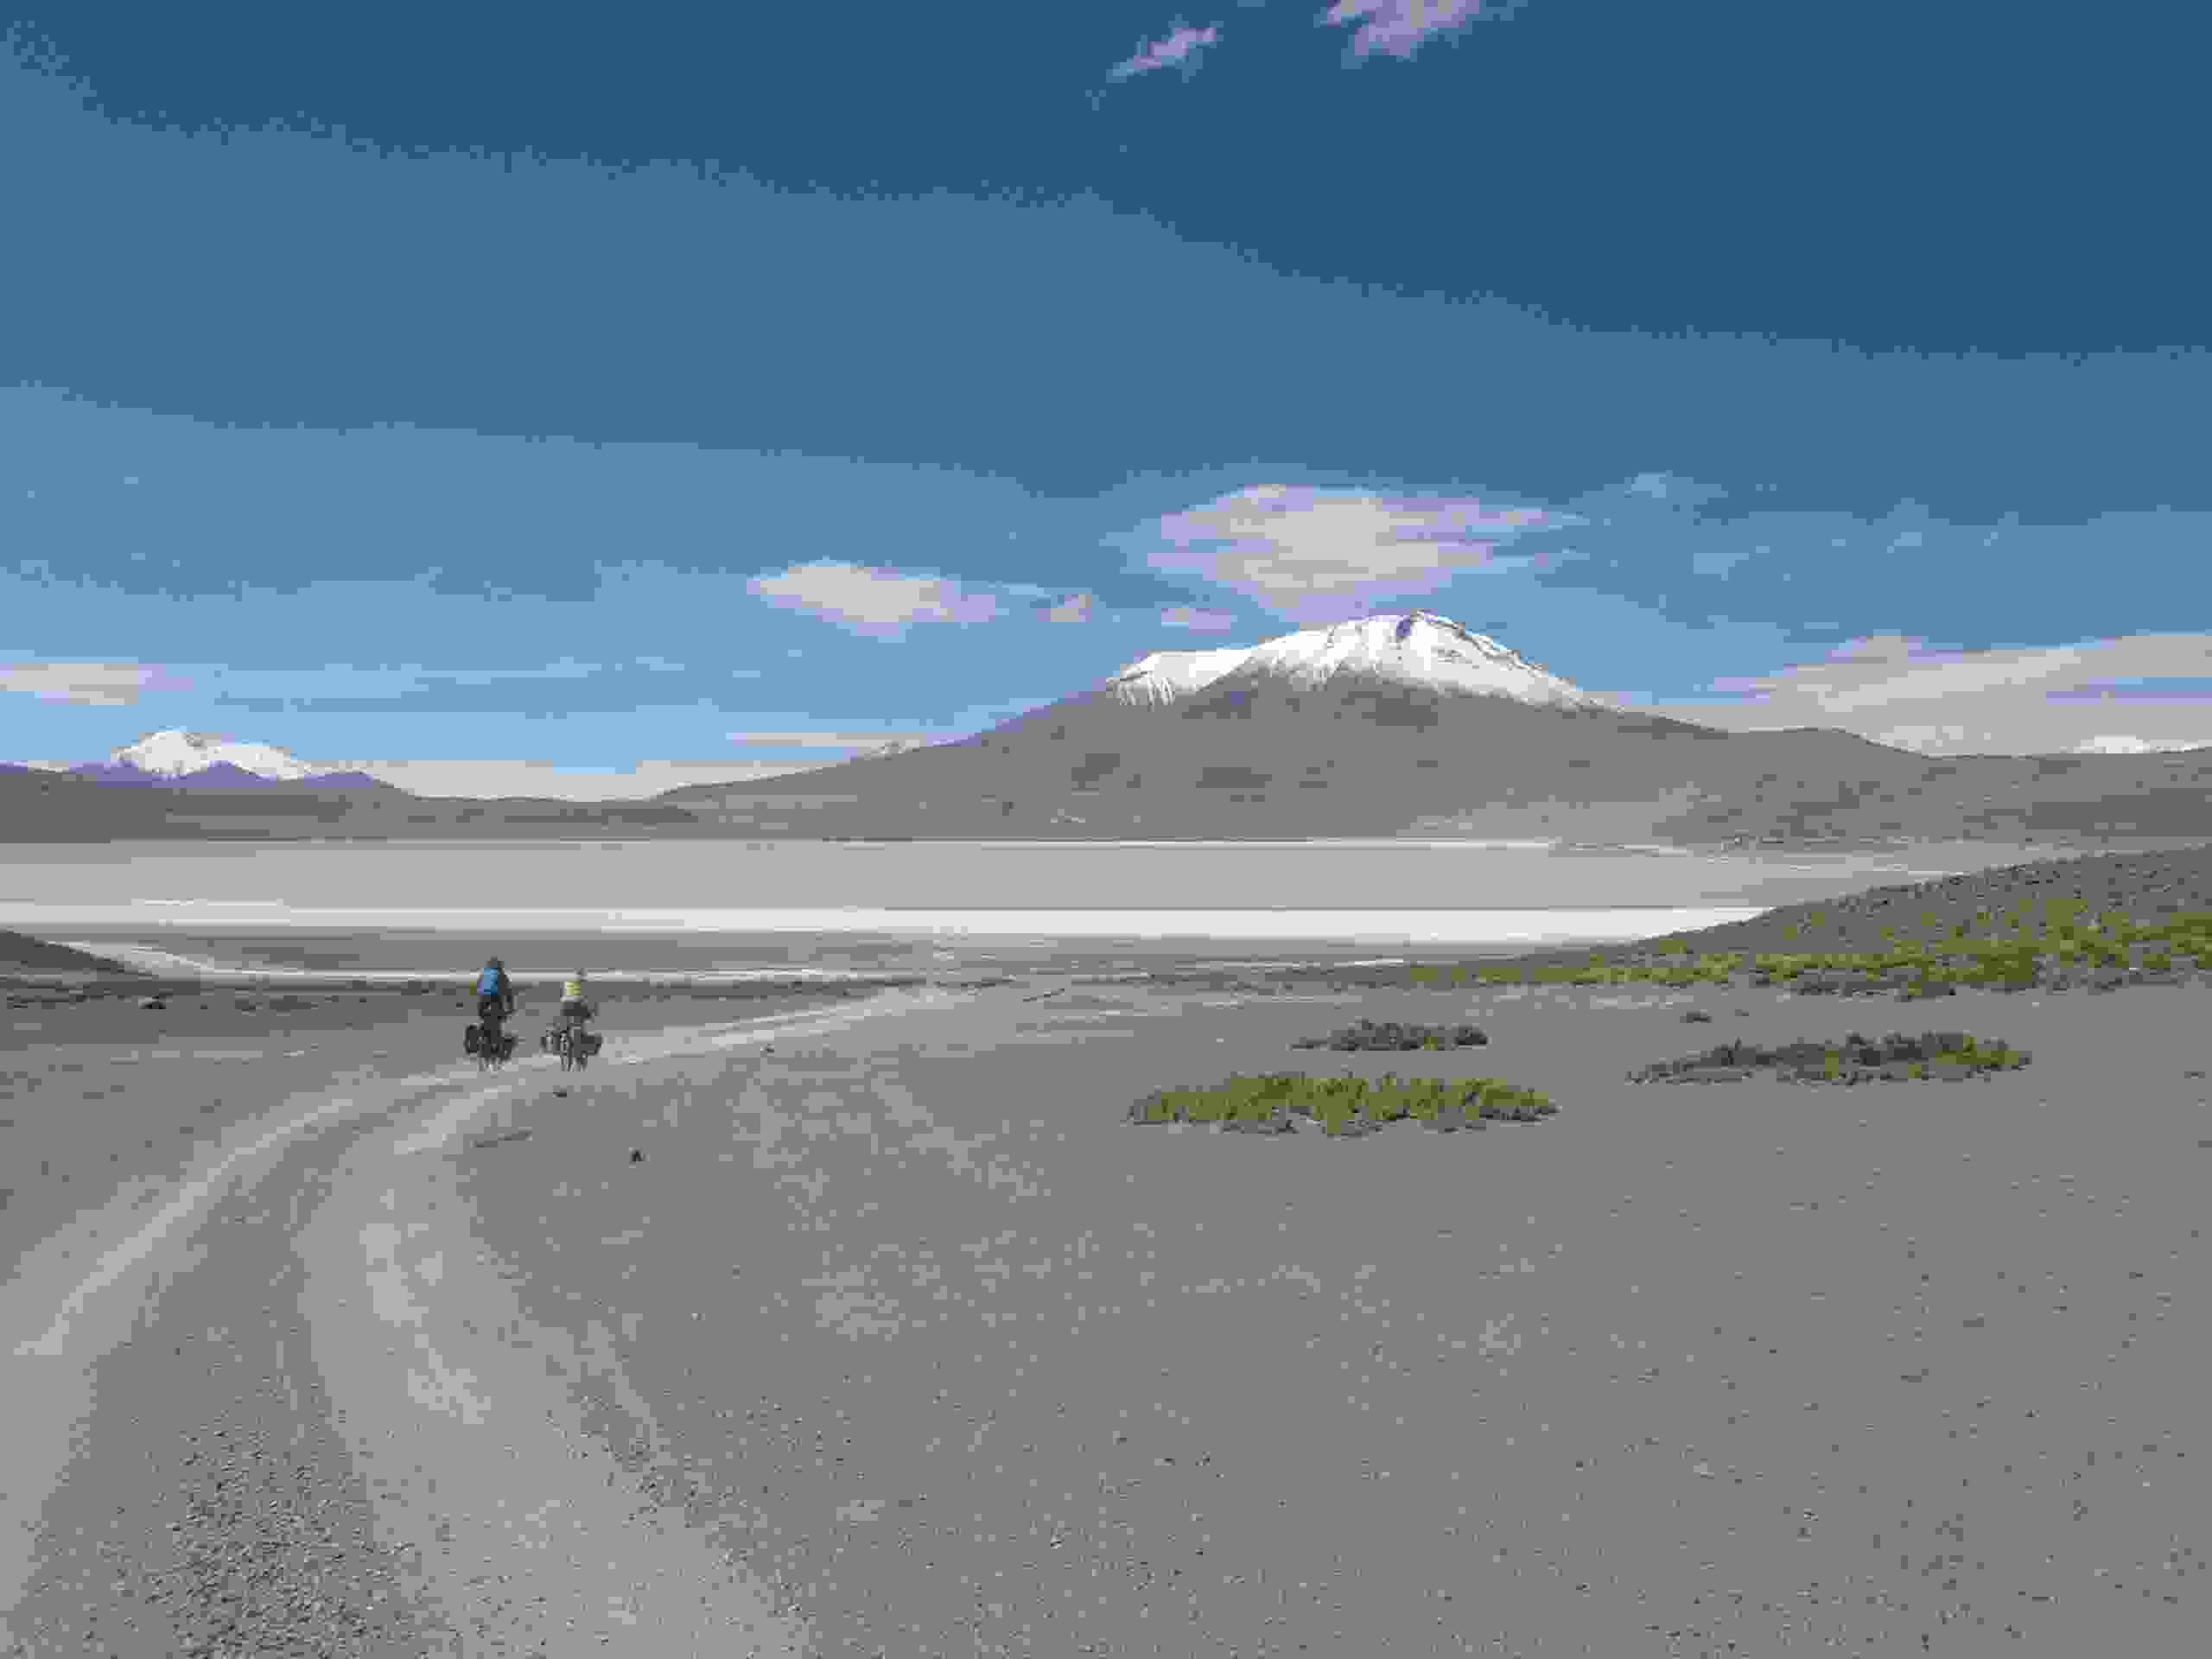
\includegraphics[width=\mywidth]{../wp-content/uploads/2015/04/wpid-wp-1427985384246.jpg} \end{center}

 Pour terminer à la Laguna Hedionda.
\begin{center} 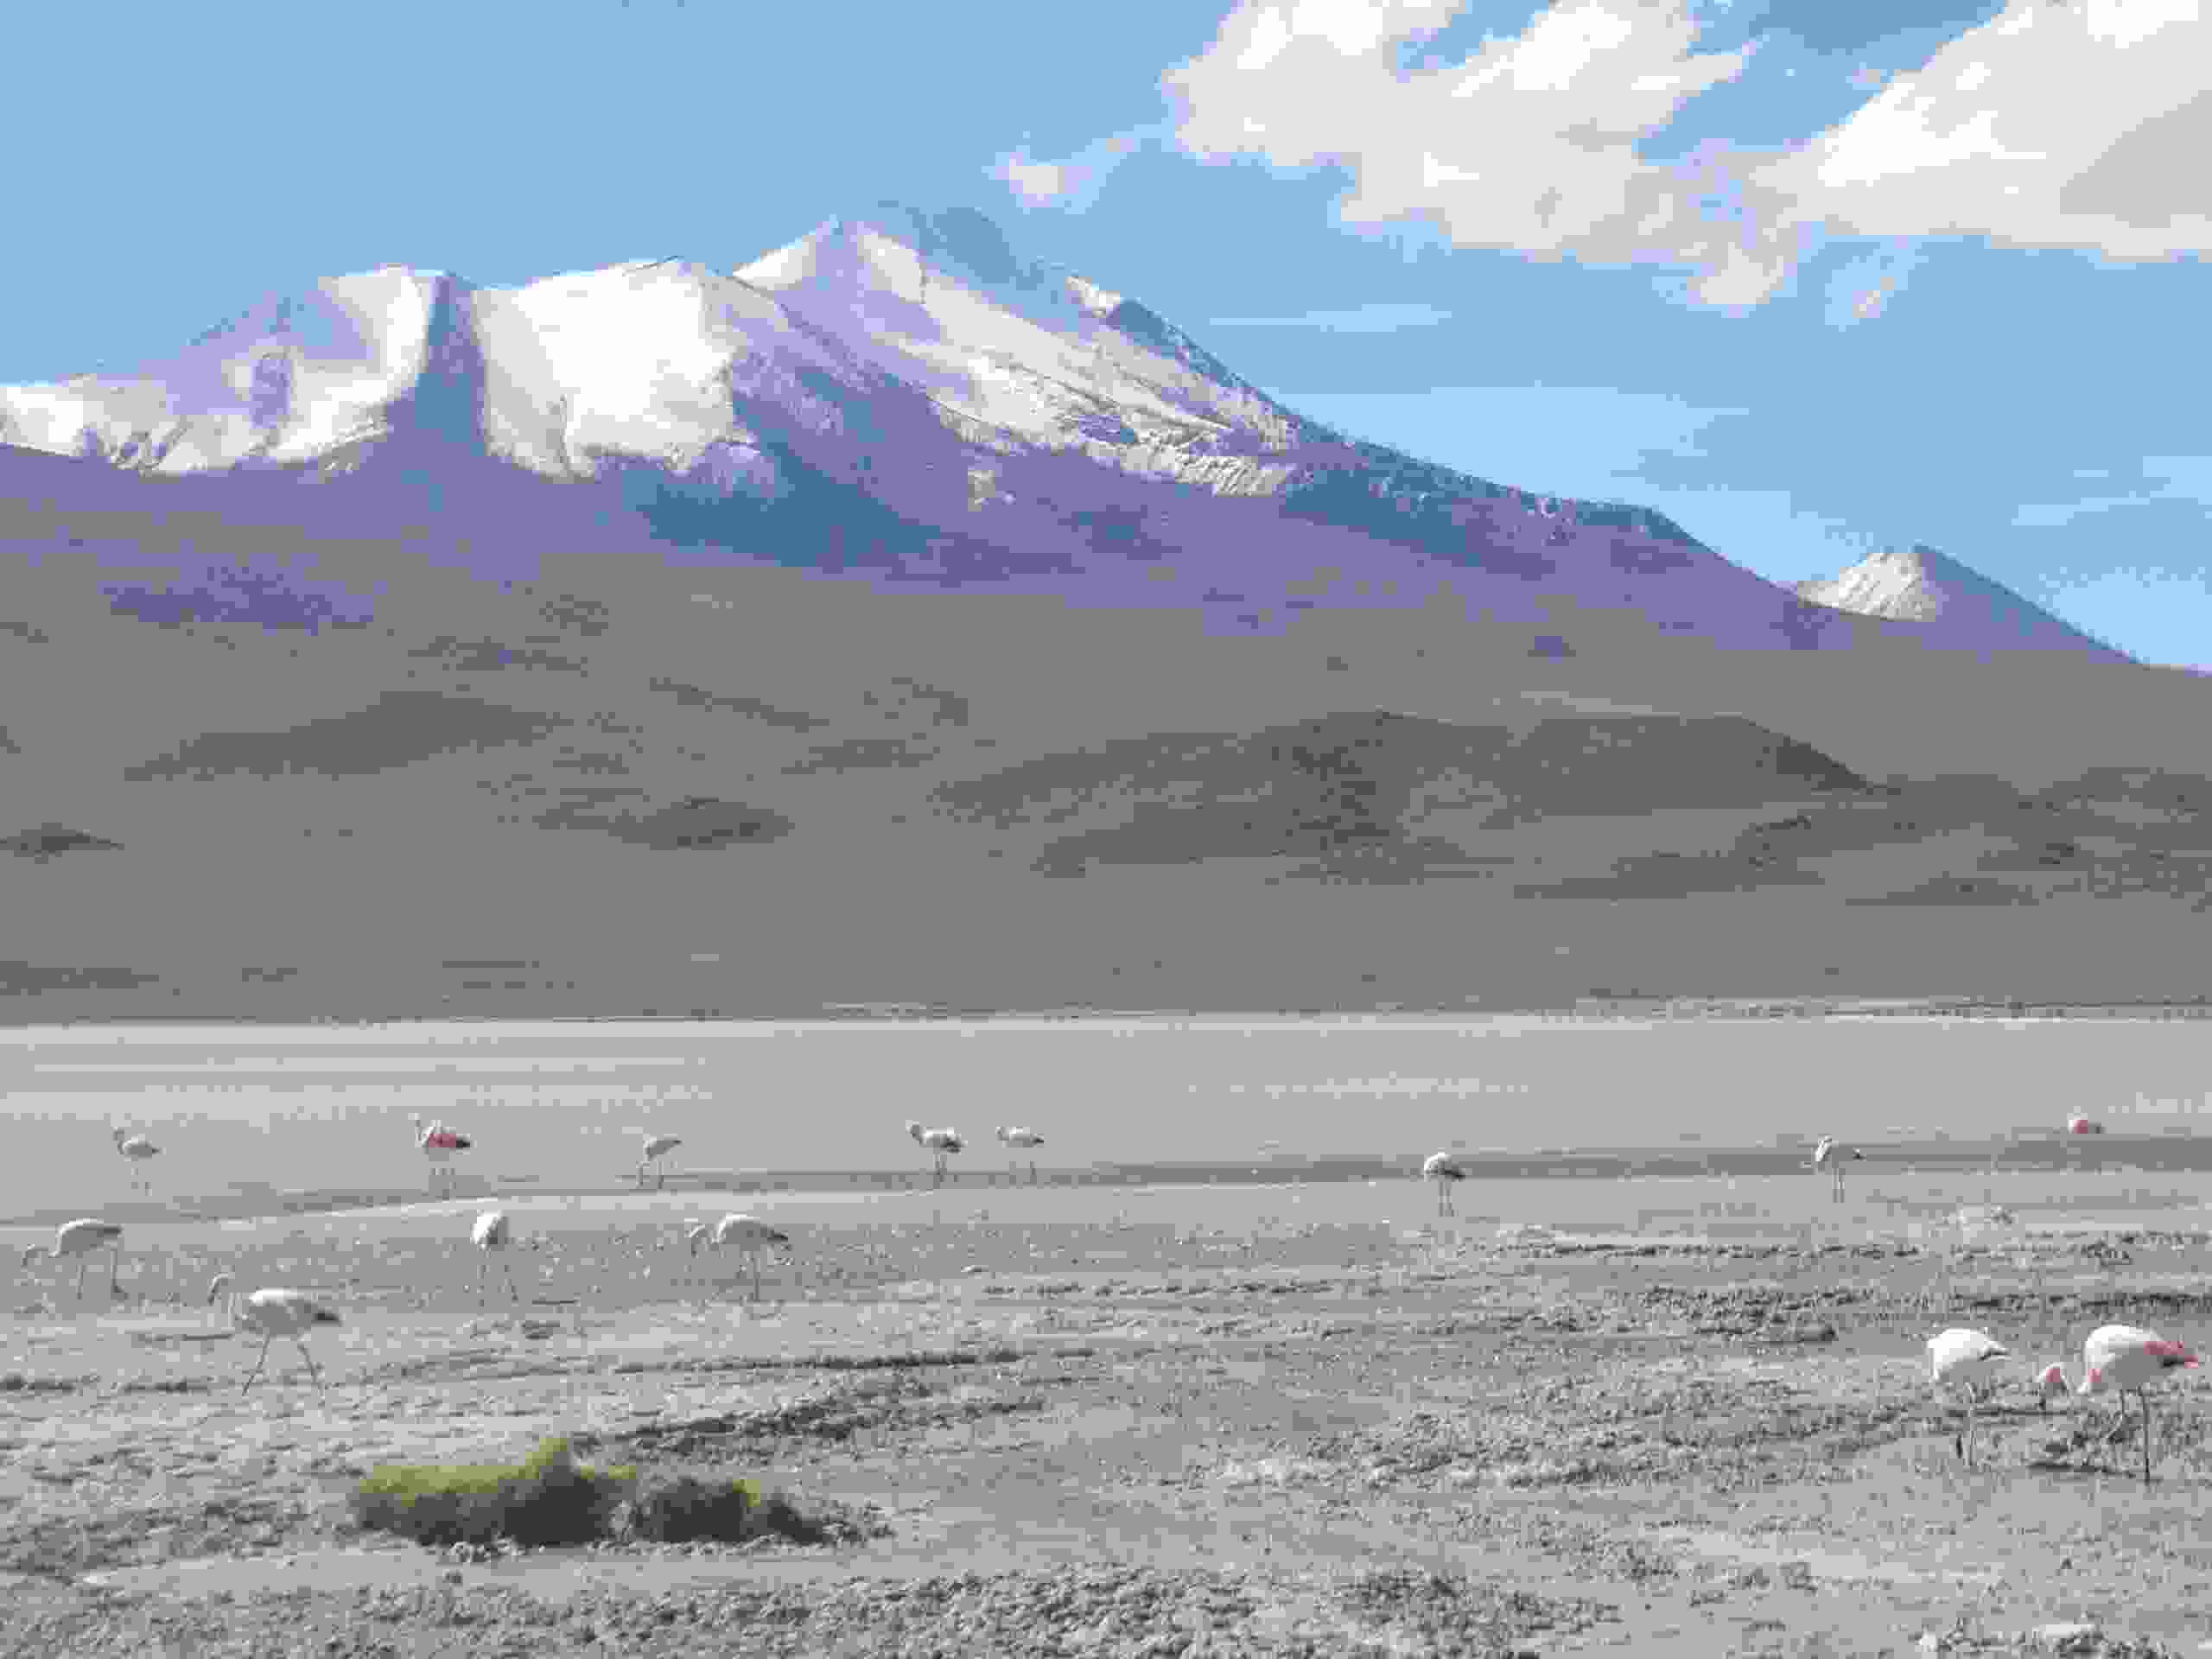
\includegraphics[width=\mywidth]{../wp-content/uploads/2015/04/wpid-wp-1427985428387.jpg} \end{center}
\begin{center} 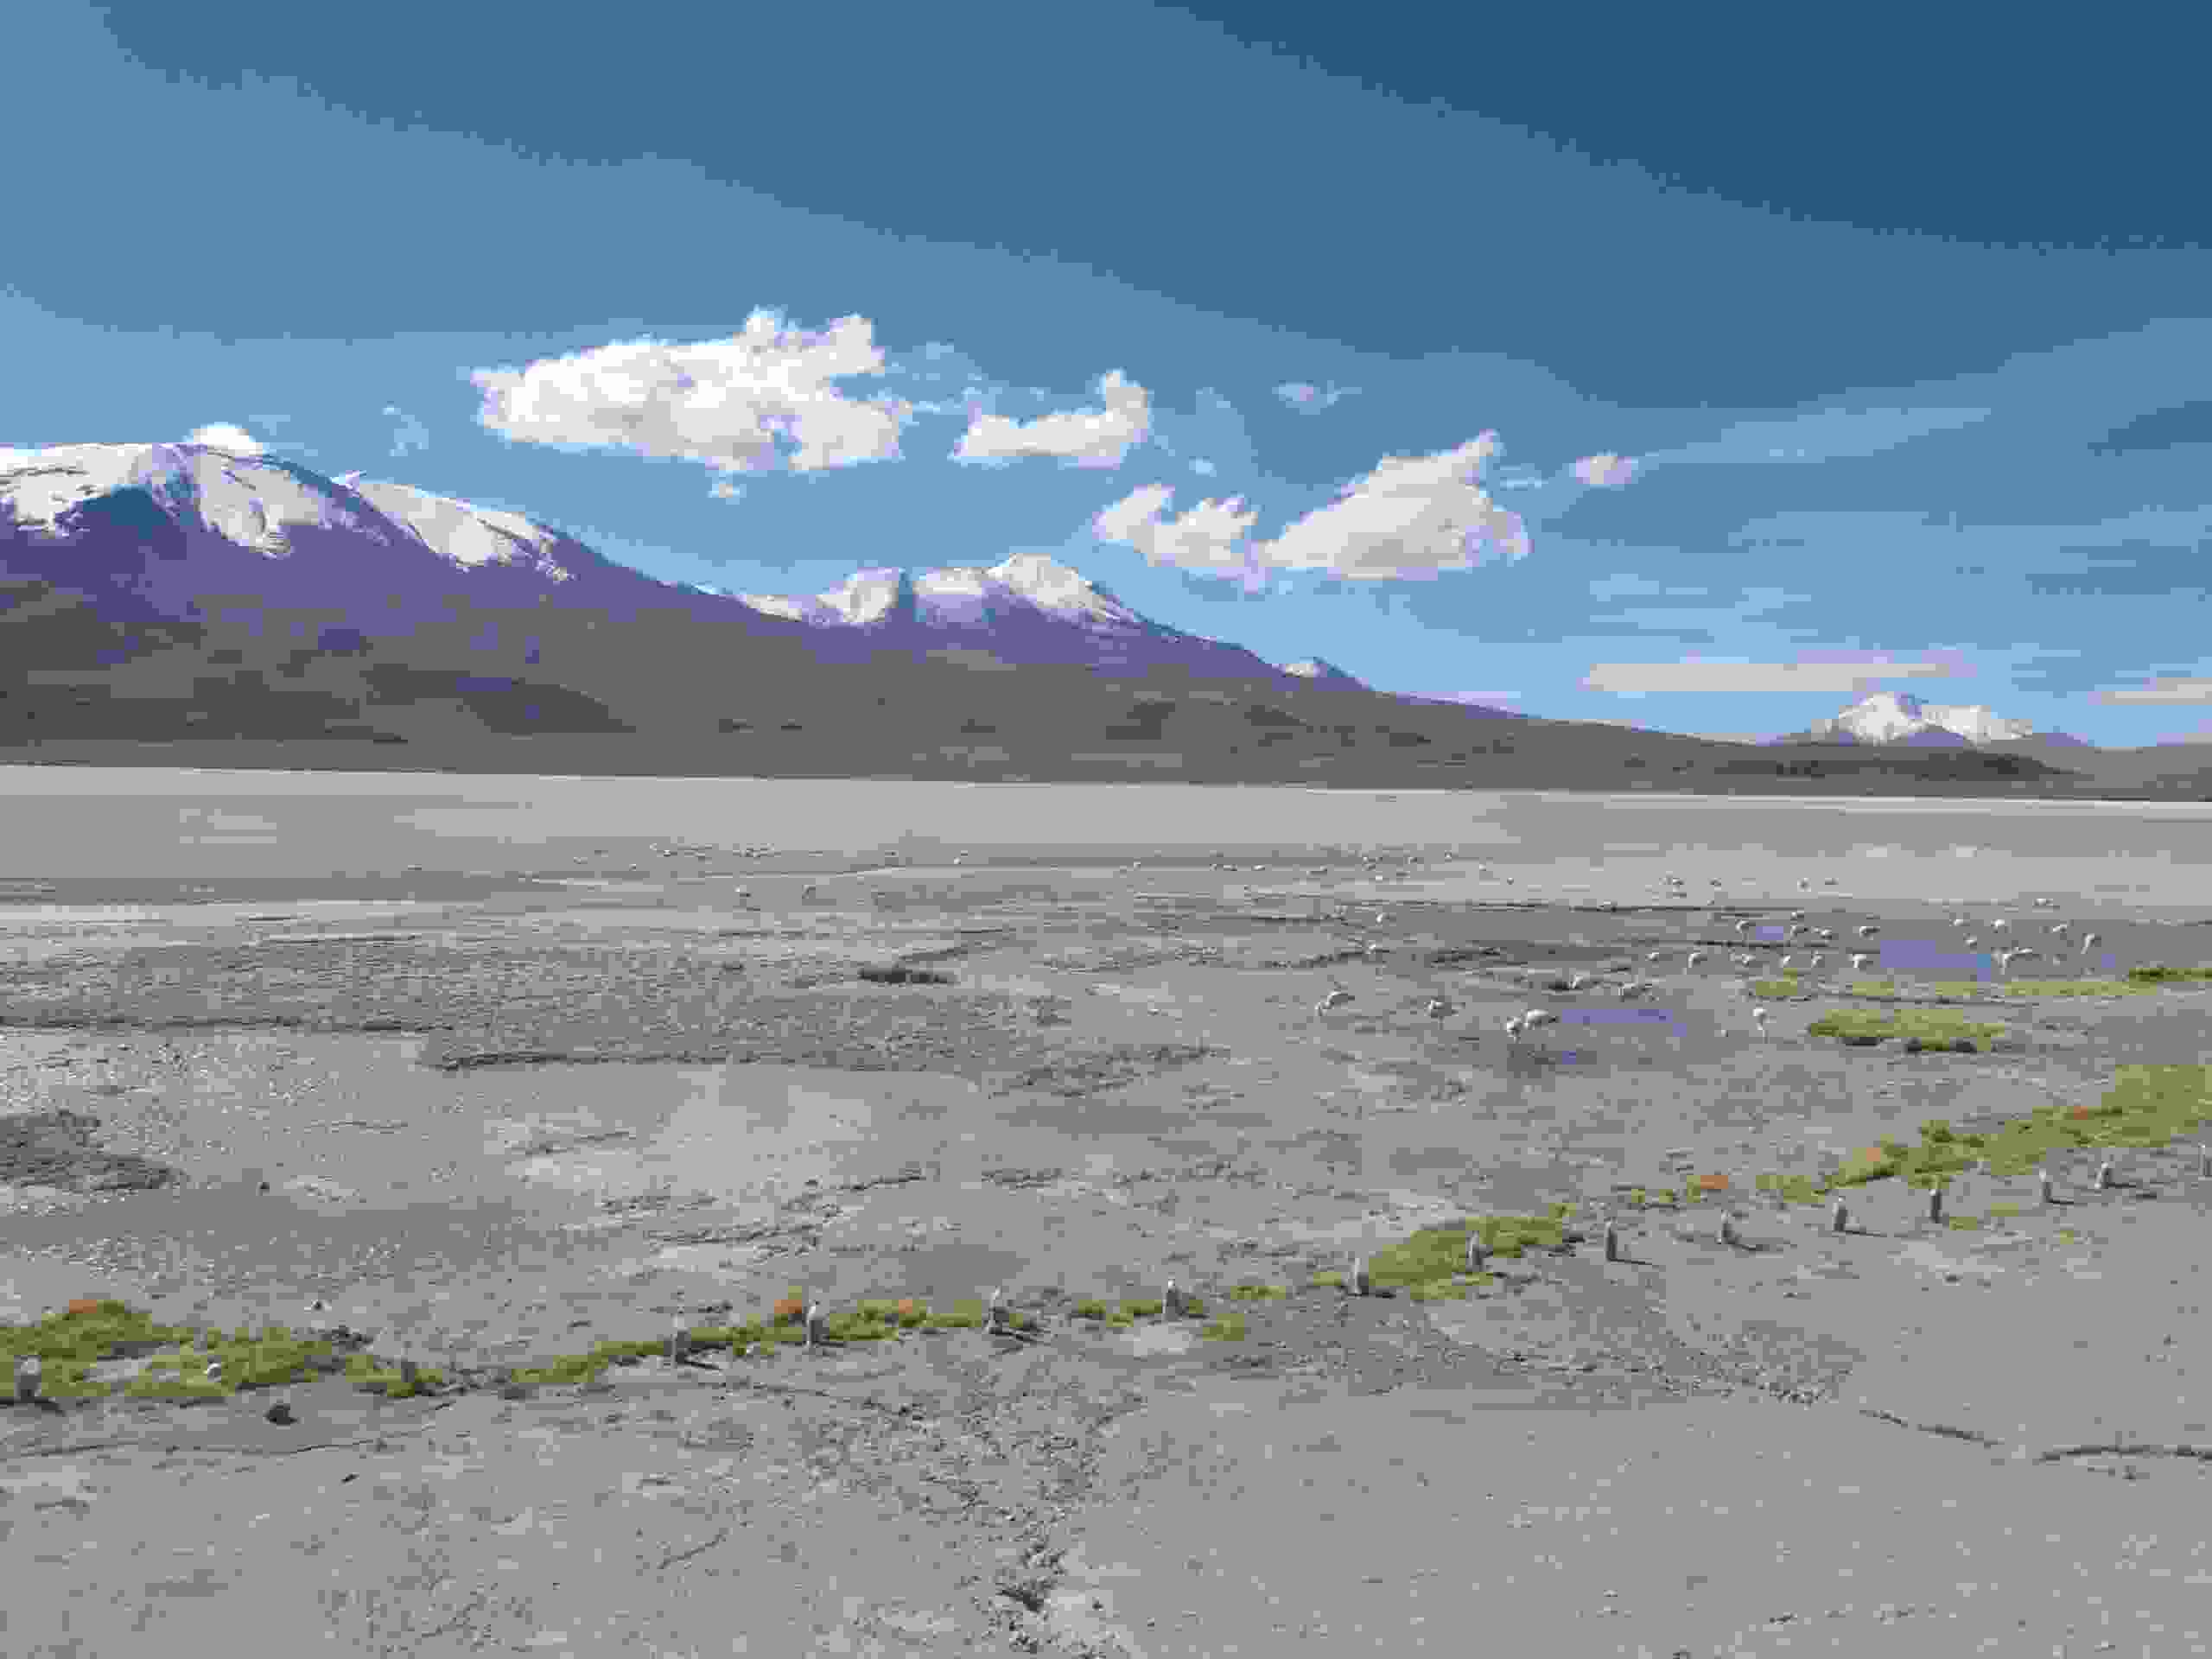
\includegraphics[width=\mywidth]{../wp-content/uploads/2015/04/wpid-wp-1427985446476.jpg} \end{center}
\begin{center} 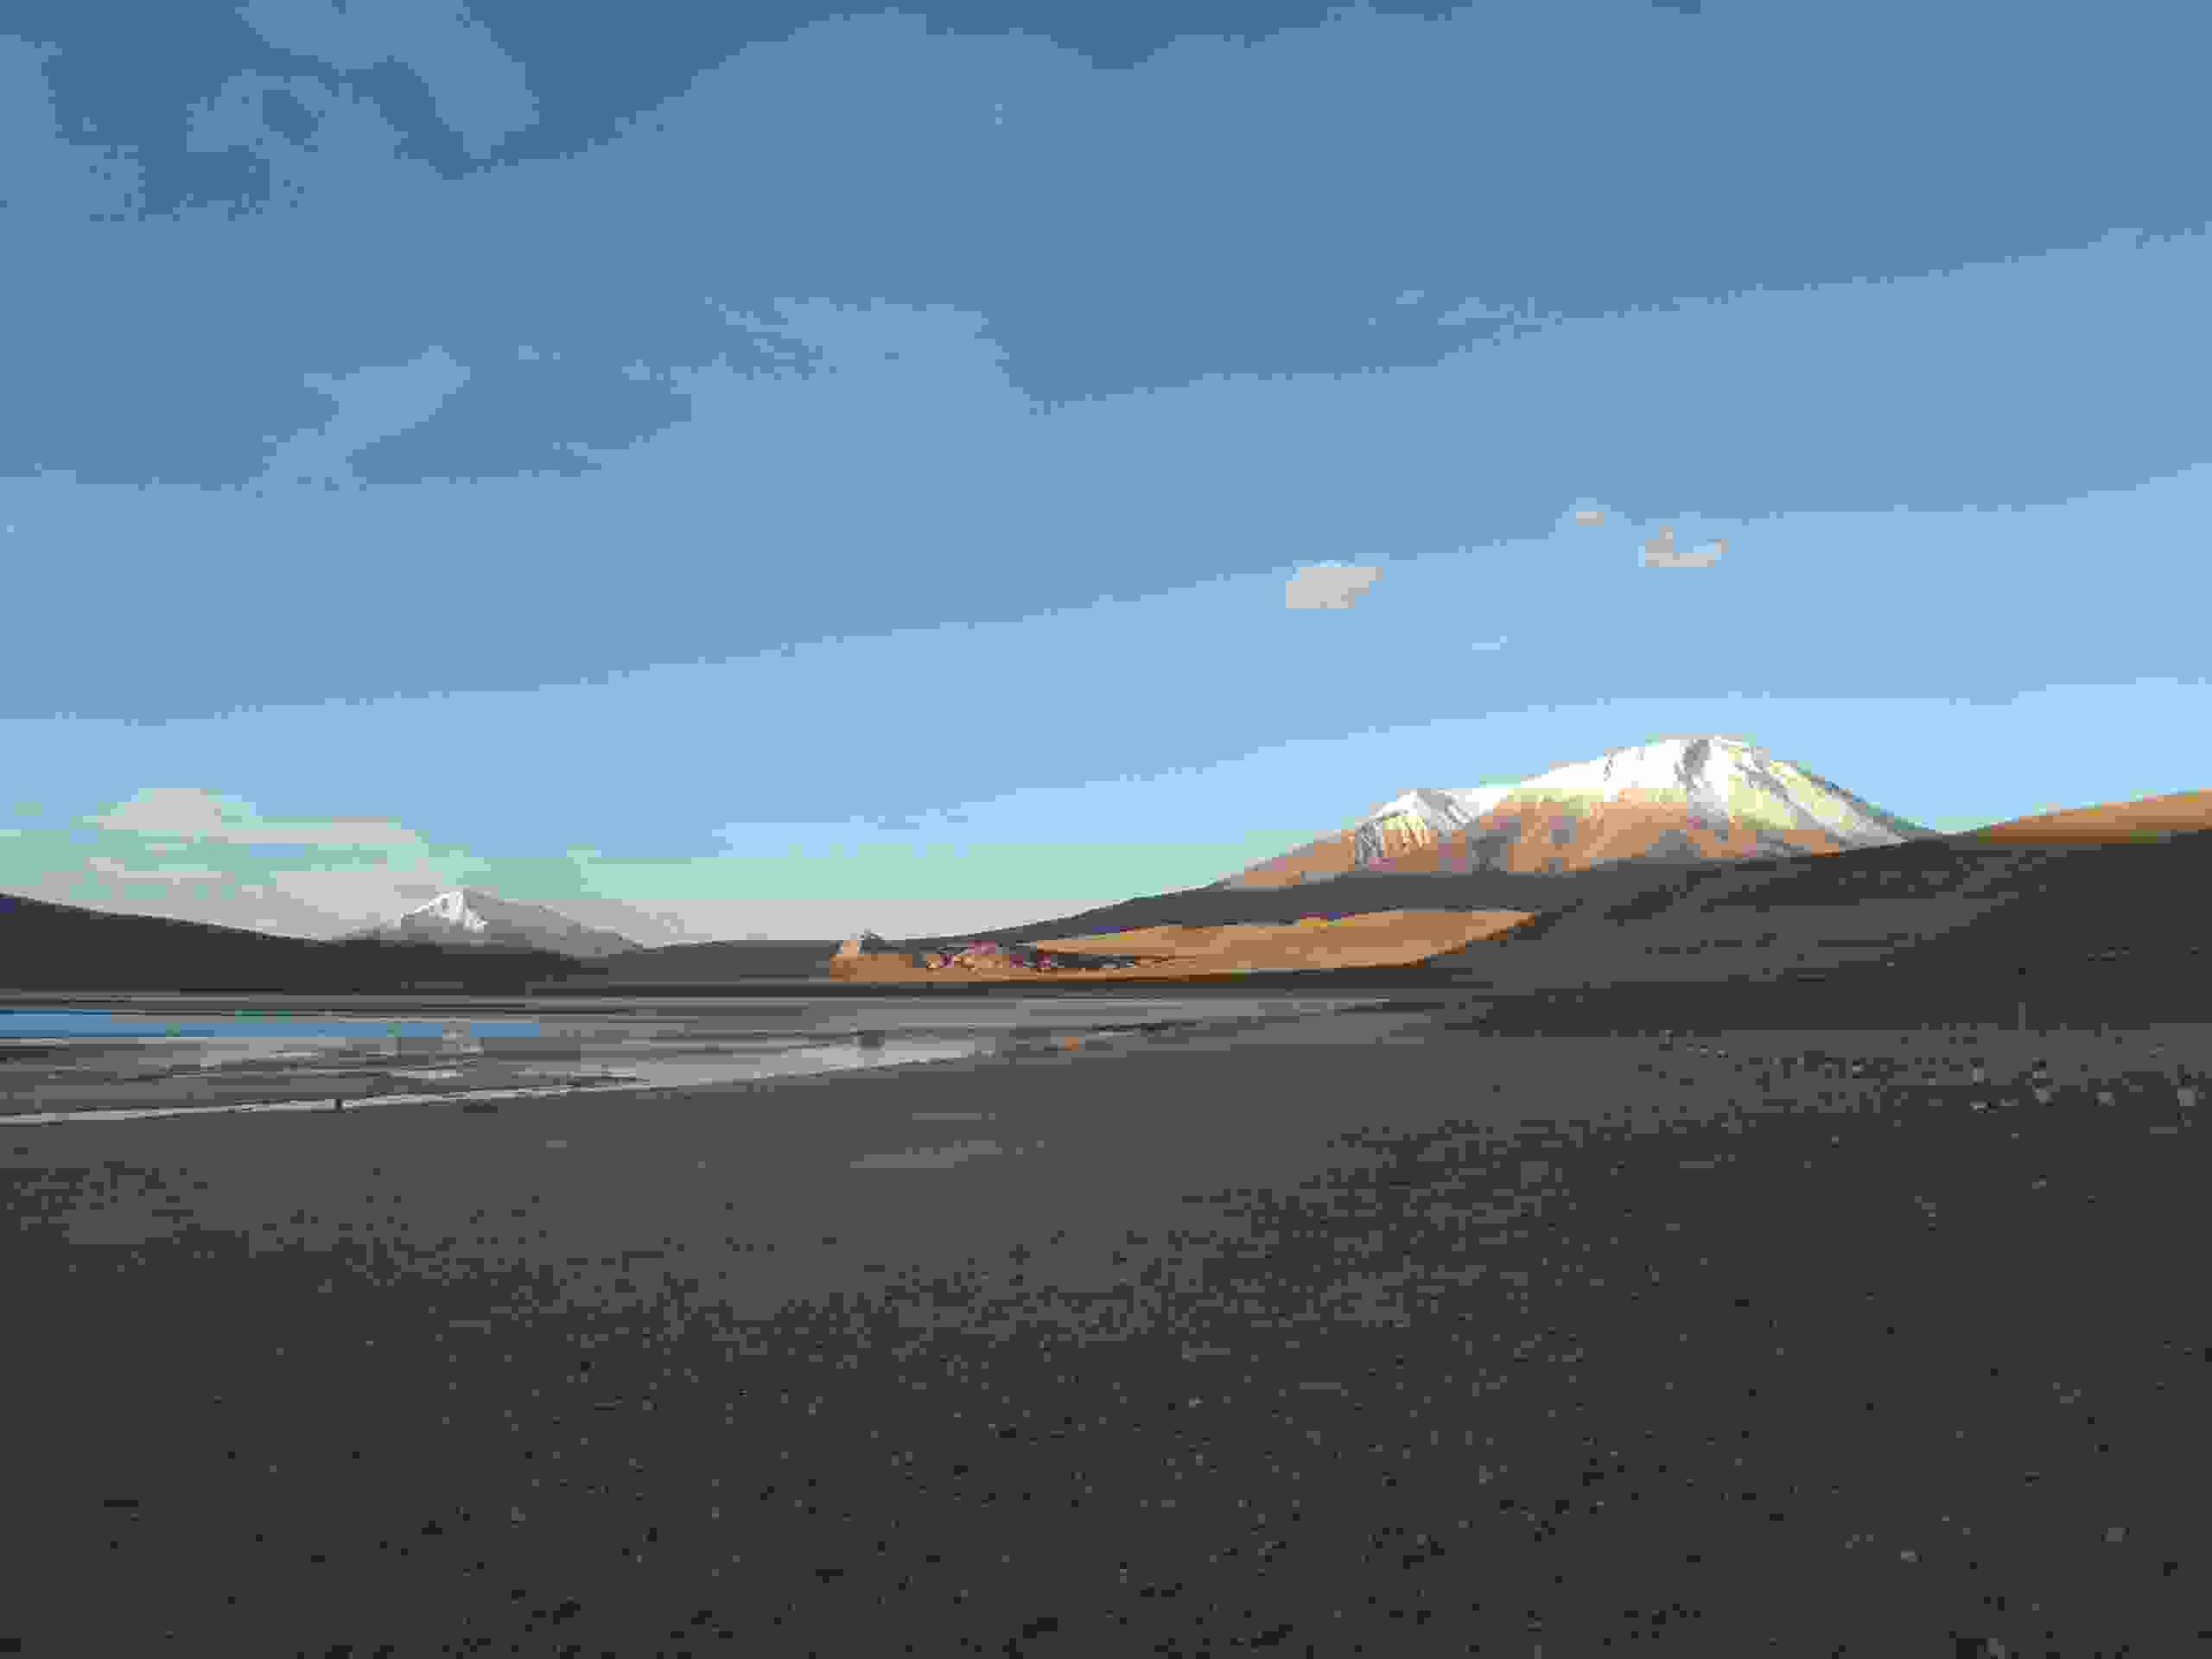
\includegraphics[width=\mywidth]{../wp-content/uploads/2015/04/wpid-wp-1427985493186.jpg} \end{center}
\begin{center} 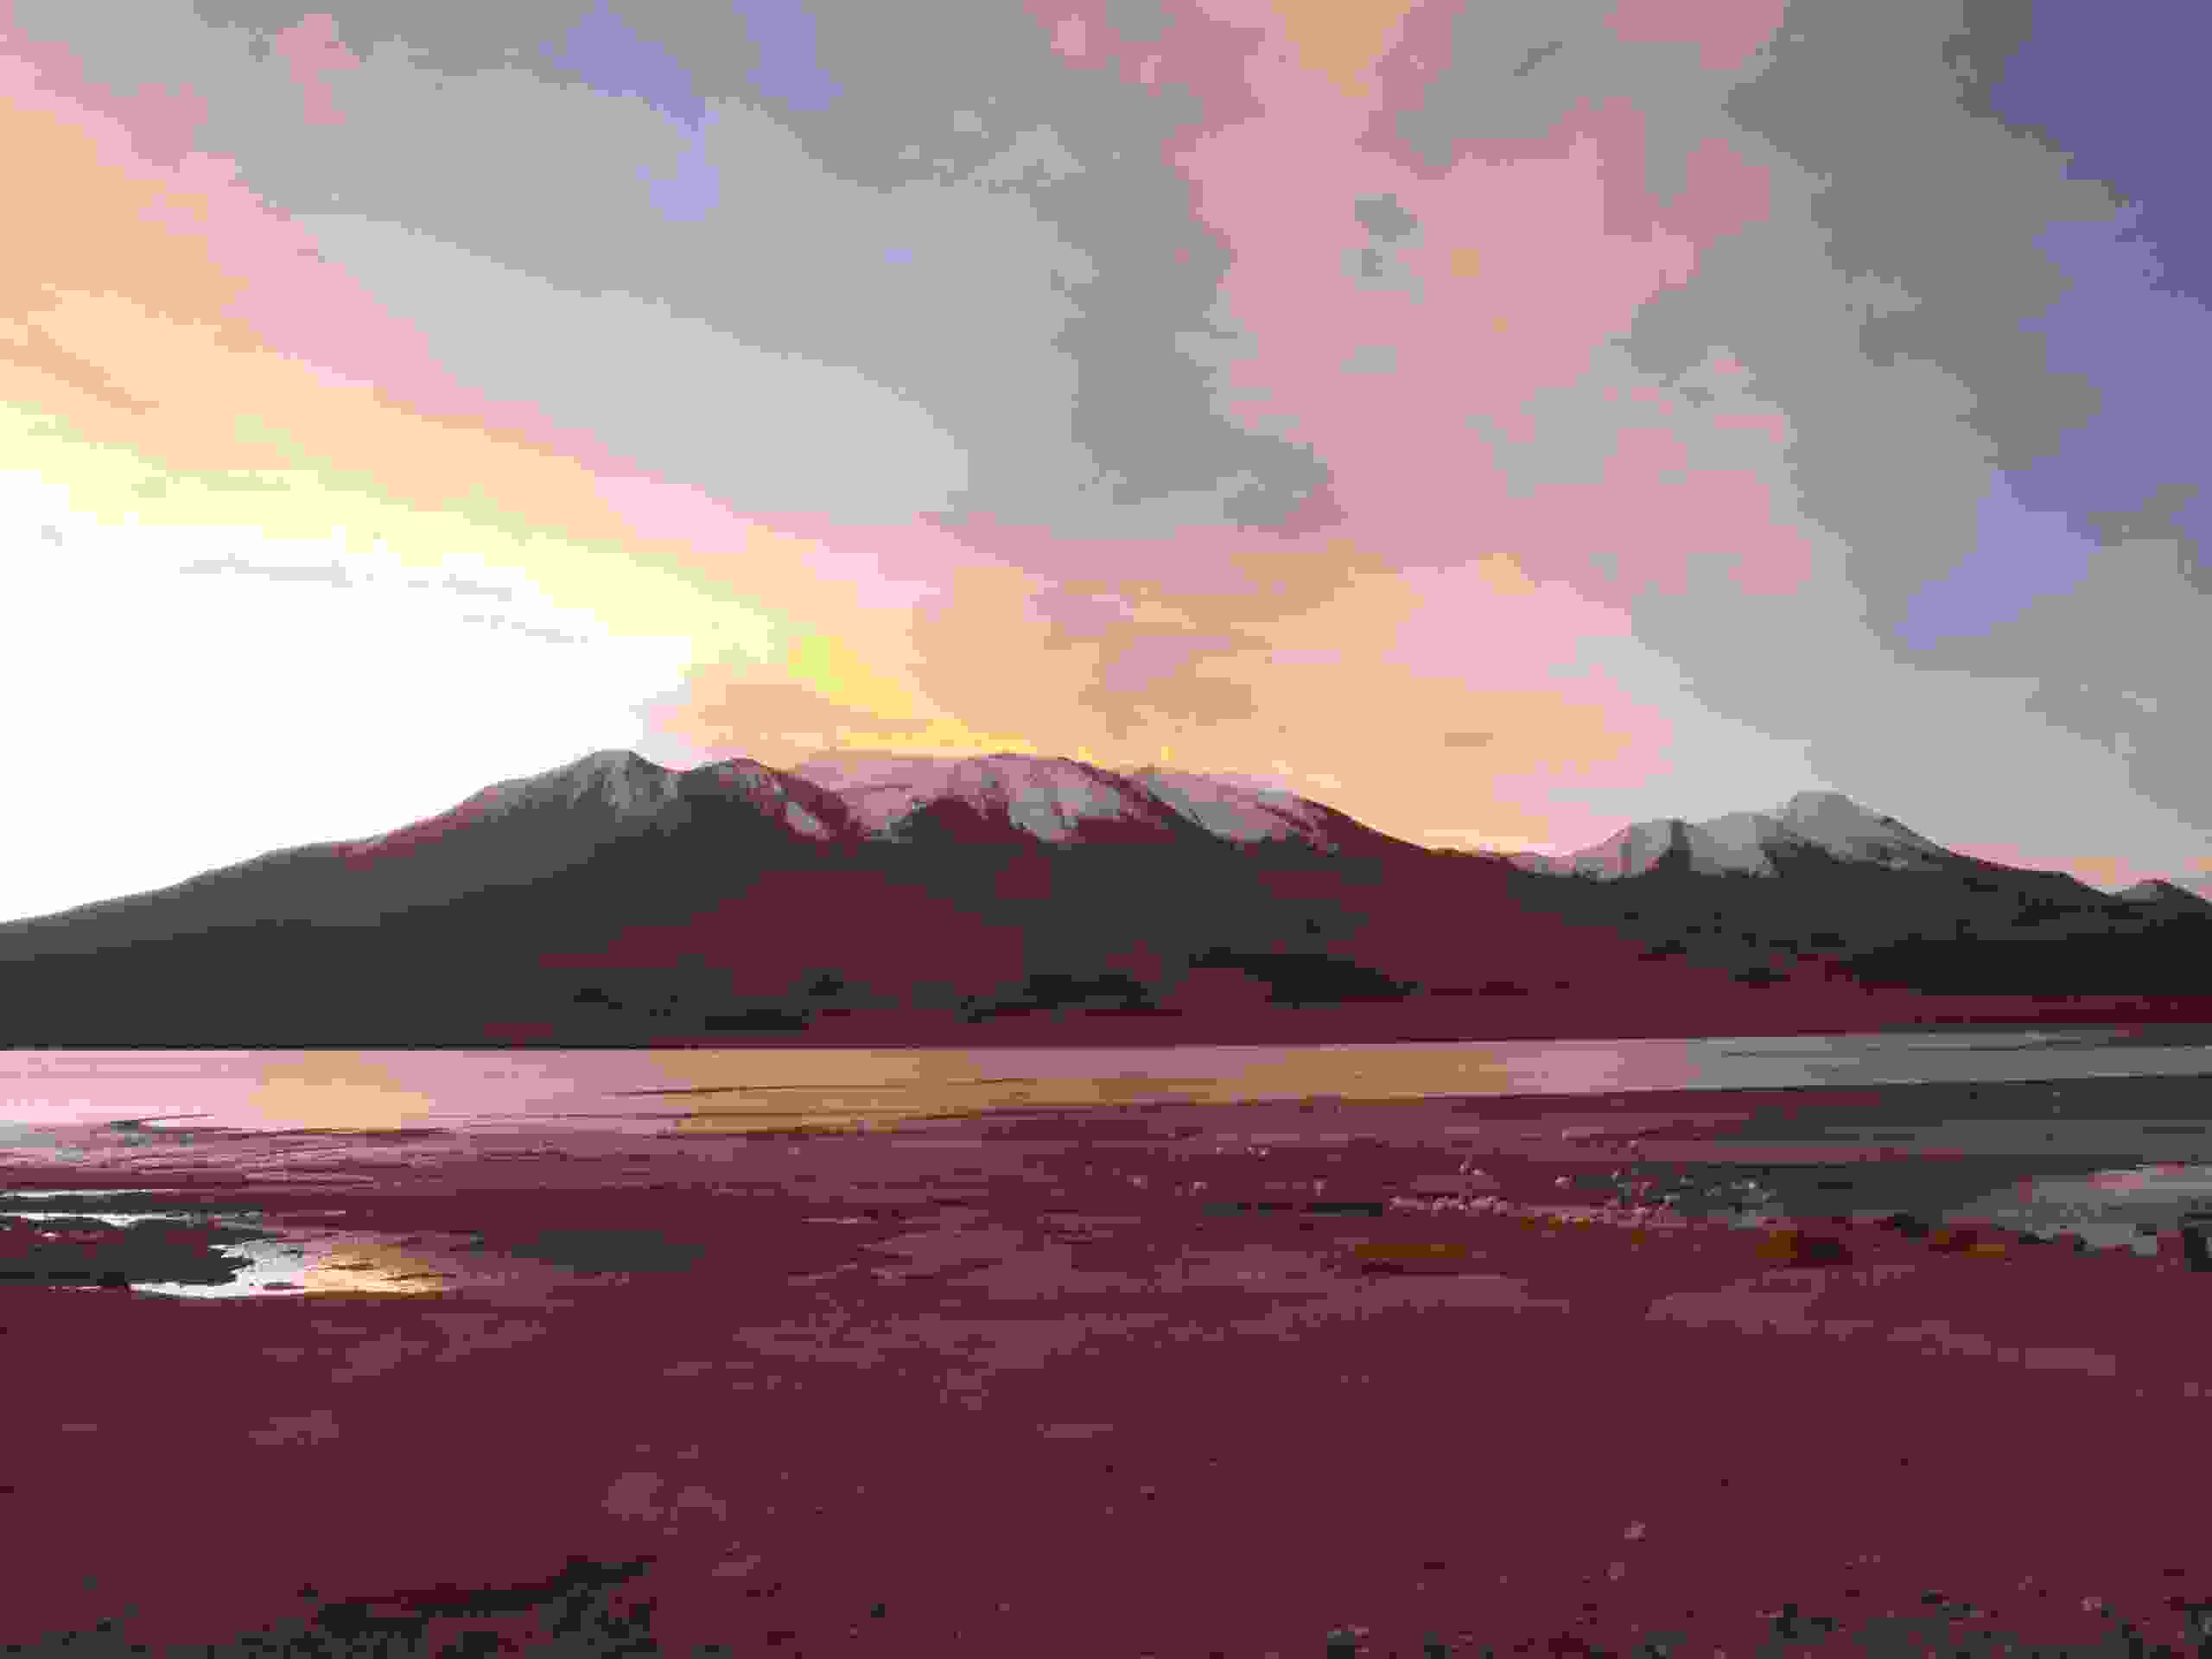
\includegraphics[width=\mywidth]{../wp-content/uploads/2015/04/wpid-wp-1427985509761.jpg} \end{center}

 \subsection*{8\ieme\ jour} 

 Encore de la piste entre sable, cailloux et tôle ondulée :
\begin{center} 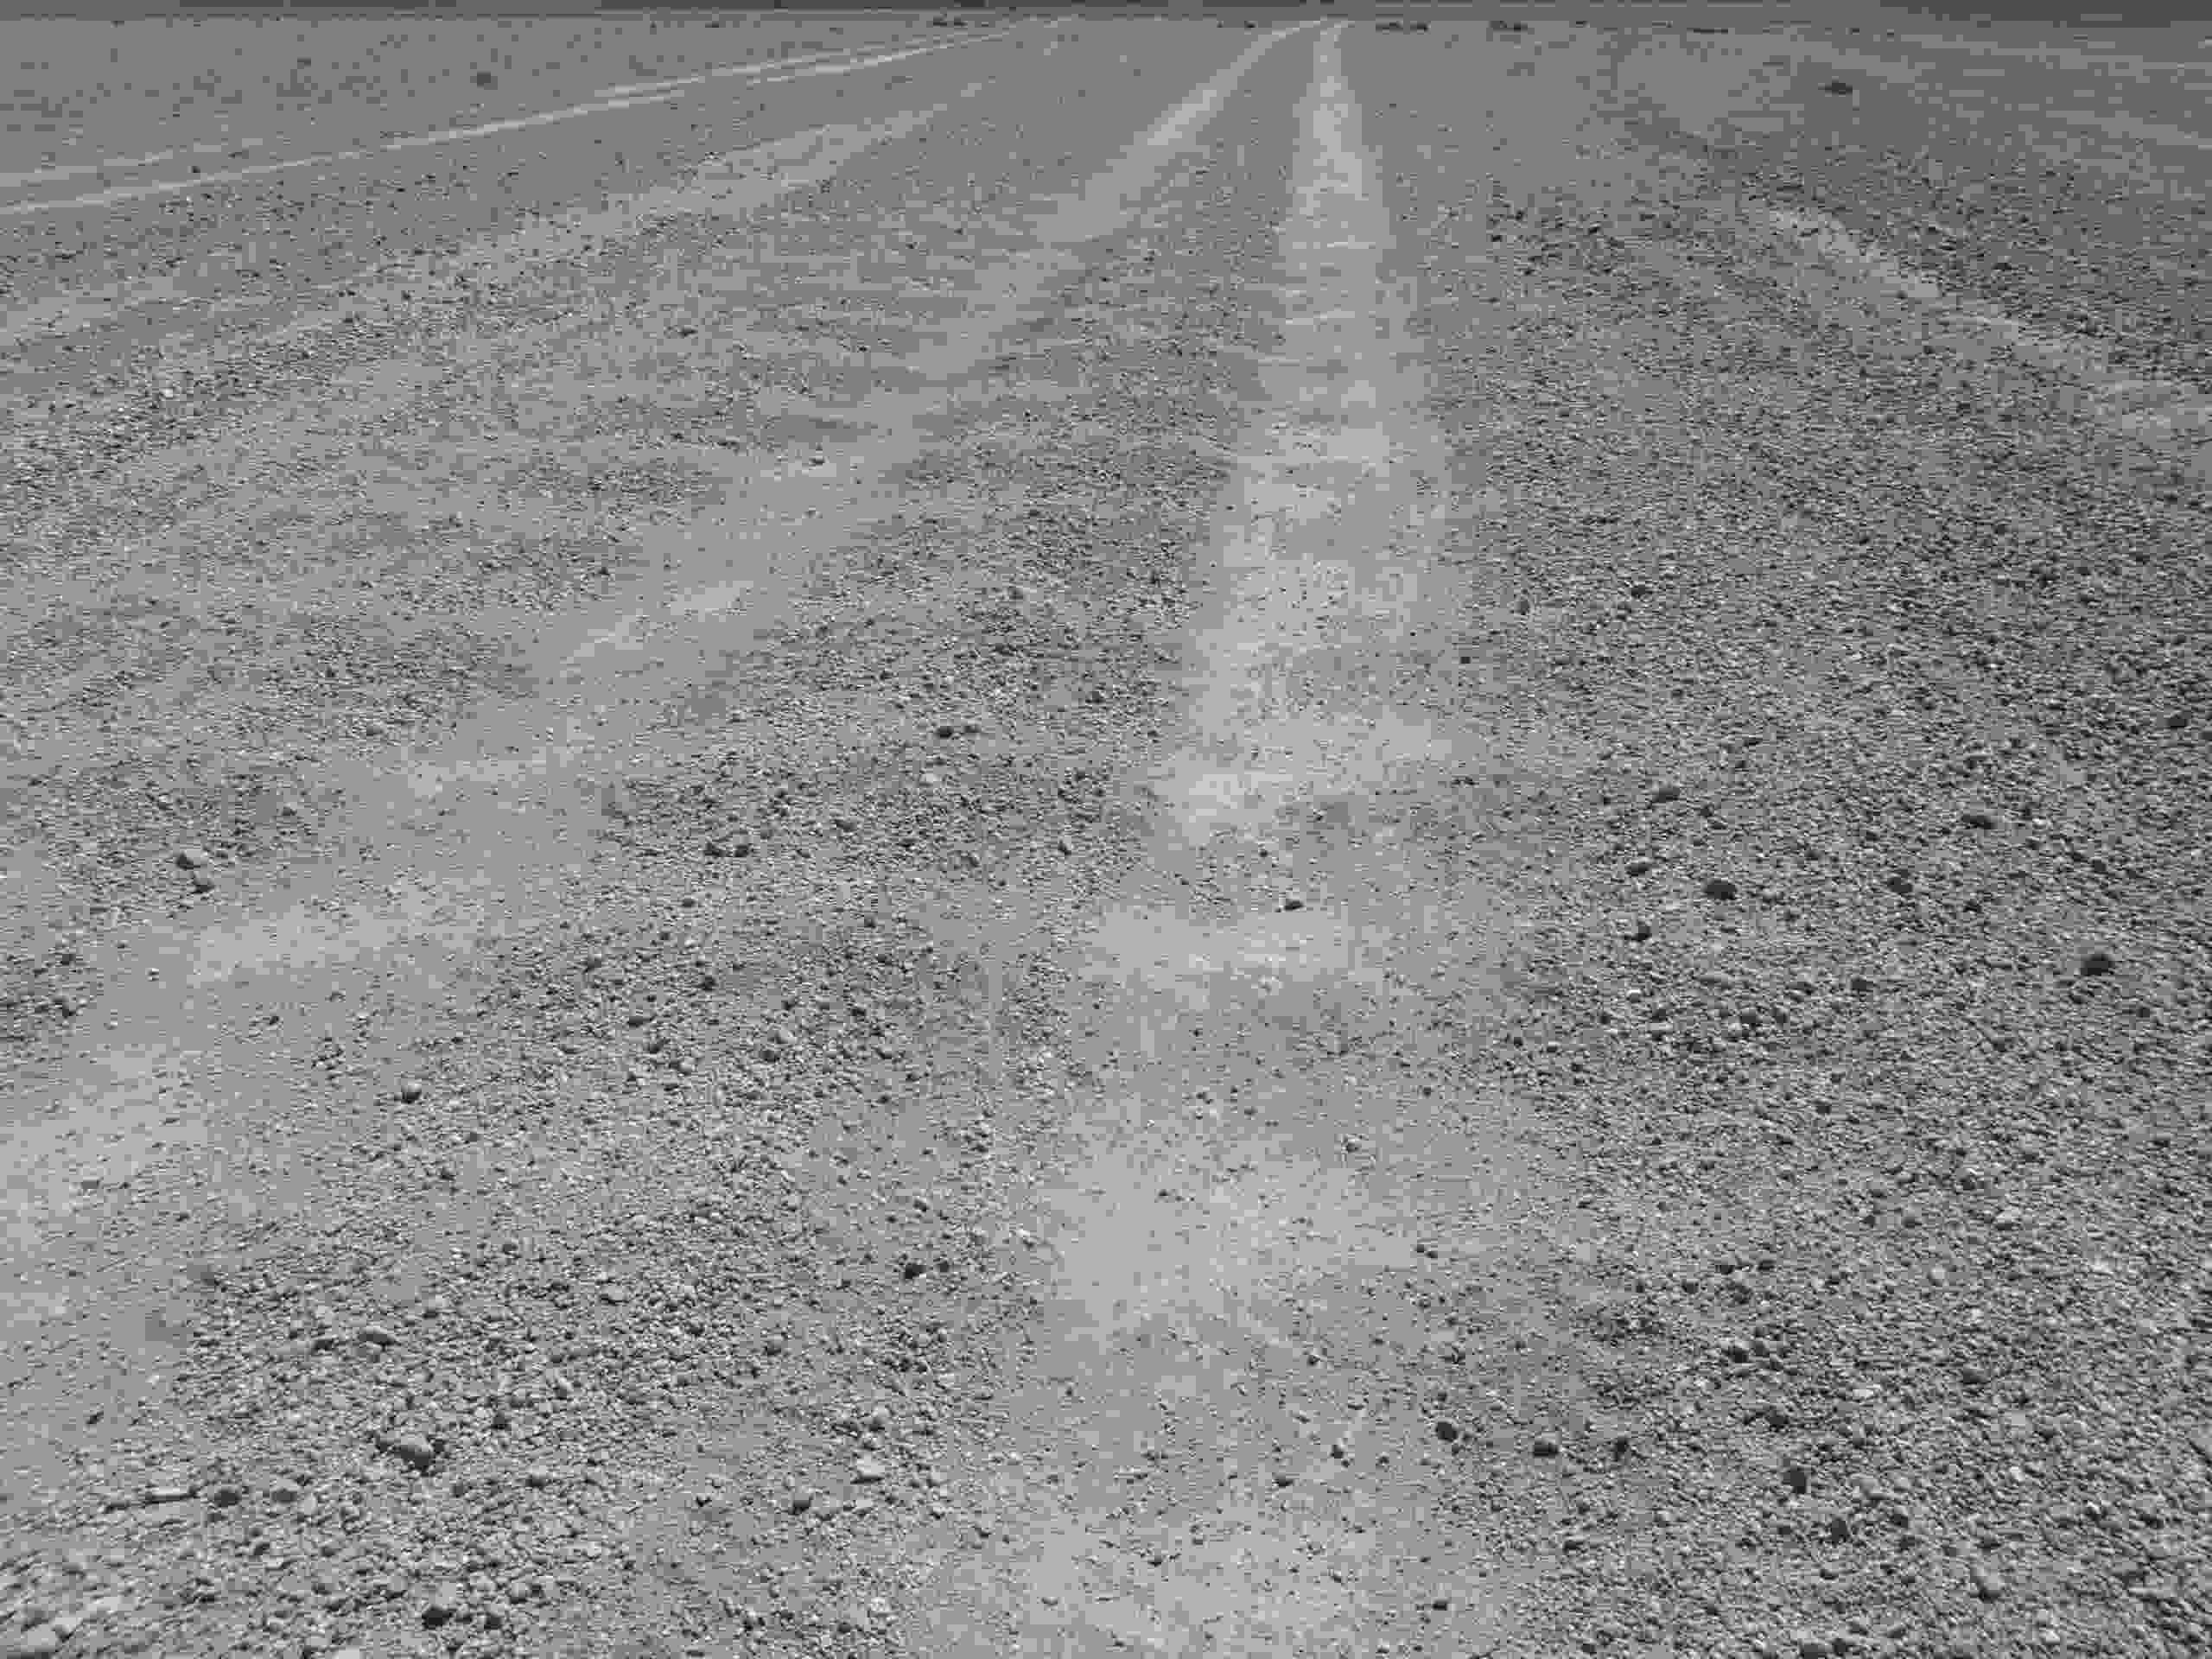
\includegraphics[width=\mywidth]{../wp-content/uploads/2015/04/wpid-wp-1427985527818.jpg} \end{center}

\pagebreak
 On longe un dernier lac.
\begin{center} \includegraphics[width=\mywidth]{../wp-content/uploads/2015/04/wpid-wp-1427985559421.jpg} \end{center}
\begin{center} \includegraphics[width=\mywidth]{../wp-content/uploads/2015/04/wpid-wp-1427985574067.jpg} \end{center}

 Au moment de rejoindre la première route en bon état depuis un moment, on se fait dépasser par un cycliste anglais : c'est seulement son 5e jour depuis San Pedro. 

\pagebreak
 Dans la foulée on rencontre 2 autres cyclistes qui empruntent la route principale : quasiment un peloton pendant quelques kilomètres !
\begin{center} \includegraphics[width=\mywidth]{../wp-content/uploads/2015/04/wpid-wp-1427985593533.jpg} \end{center}
\begin{center} \includegraphics[width=\mywidth]{../wp-content/uploads/2015/04/wpid-wp-1427985630834.jpg} \end{center}

\pagebreak
 La journée se termine par un dernier petit col à 4200m.
\begin{center} \includegraphics[width=\mywidth]{../wp-content/uploads/2015/04/wpid-wp-1427985662568.jpg} \end{center}

 \subsection*{9\ieme\ jour} 

 Longue descente dans le sable.
\begin{center} \includegraphics[width=\mywidth]{../wp-content/uploads/2015/04/wpid-wp-1427985680592.jpg} \end{center}
\begin{center} \includegraphics[width=\mywidth]{../wp-content/uploads/2015/04/wpid-wp-1427985709669.jpg} \end{center}
\begin{center} \includegraphics[width=\mywidth]{../wp-content/uploads/2015/04/wpid-wp-1427985731653.jpg} \end{center}

\pagebreak
 Traversée d'un petit salar.
\begin{center} \includegraphics[width=\mywidth]{../wp-content/uploads/2015/04/wpid-wp-1427985755004.jpg} \end{center}

 À la pause de midi on croise un cycliste autrichien. Pour lui c'est le début, bon courage !
\begin{center} \includegraphics[width=\mywidth]{../wp-content/uploads/2015/04/wpid-wp-1427985769783.jpg} \end{center}

\pagebreak
 Du plat pour finir la journée le long des champs de quinoa, on est bien en Bolivie.
\begin{center} \includegraphics[width=\mywidth]{../wp-content/uploads/2015/04/wpid-wp-1427985789893.jpg} \end{center}

 La traversée du Sud Lipez se termine dans le village de San Juan.
\begin{center} \includegraphics[width=\mywidth]{../wp-content/uploads/2015/04/wpid-wp-1427985851009.jpg} \end{center}

\pagebreak
 Un poulet frites riz le plat numéro 1 en Bolivie : ça change des pâtes, sauce tomate, thon…
\begin{center} \includegraphics[width=\mywidth]{../wp-content/uploads/2015/04/wpid-wp-1427985818141.jpg} \end{center}
